\documentclass[11pt,oneside]{article}

\usepackage[a4paper,margin=27mm,headheight=15pt]{geometry}
\usepackage[T1]{fontenc}
\usepackage[utf8]{inputenc}
\IfFileExists{libertinus.sty}{\usepackage{libertinus}}{\usepackage{lmodern}}
\usepackage{microtype}
\usepackage{amsmath,amssymb,amsthm,mathtools,mathrsfs}
\usepackage{bm}
\usepackage{booktabs,longtable,array,tabularx}
\usepackage{graphicx}
\usepackage{pgfplots}
\usepackage{xcolor}
\usepackage{enumitem}
\usepackage{fancyhdr}
\usepackage{titlesec}
\usepackage{listings}
\usepackage{xurl}
\usepackage[hypertexnames=false]{hyperref}
\usepackage[nameinlink,noabbrev]{cleveref}

\definecolor{linkblue}{RGB}{25,75,135}
\definecolor{shadegray}{RGB}{246,247,249}
\definecolor{rulegray}{RGB}{195,201,208}
\pgfplotsset{compat=1.18}
\hypersetup{
  colorlinks=true,
  linkcolor=linkblue,
  citecolor=linkblue,
  urlcolor=linkblue,
  pdftitle={The Thue--Morse Sequence: Formula Atlas and Fabius--Rvachev Frontier Results},
  pdfsubject={Formula atlas, finite-block calculus, Fourier and Laplace products, q-binomial extrapolation, and Lean crosswalks},
  pdfkeywords={Thue-Morse, Prouhet, binary digit sum, Lucas theorem, Kummer theorem, Pascal triangle, Mahler equation, Walsh transform, Riesz product, Fabius function, Rvachev up-function, sinc product, q-binomial extrapolation}
}

\pagestyle{fancy}
\fancyhf{}
\fancyhead[L]{\small Thue--Morse atlas and frontiers}
\fancyhead[R]{\small\nouppercase{\leftmark}}
\fancyfoot[C]{\thepage}
\renewcommand{\headrulewidth}{0.4pt}

\titleformat{\section}{\Large\bfseries}{\thesection}{0.7em}{}
\titleformat{\subsection}{\large\bfseries}{\thesubsection}{0.7em}{}
\titleformat{\subsubsection}{\normalsize\bfseries}{\thesubsubsection}{0.7em}{}
\setcounter{secnumdepth}{3}
\setcounter{tocdepth}{2}
\setlist[itemize]{leftmargin=2em,itemsep=0.25em,topsep=0.4em}
\setlist[enumerate]{leftmargin=2.3em,itemsep=0.25em,topsep=0.4em}
\setlength{\emergencystretch}{2em}
\allowdisplaybreaks
\numberwithin{equation}{section}

% ed.: alias counters so cleveref prints each environment's own name
% (with plain shared counters every \cref rendered as "theorem").
\usepackage{aliascnt}
\newcommand{\newsharedtheorem}[2]{%
  \newaliascnt{#1}{theorem}%
  \newtheorem{#1}[#1]{#2}%
  \aliascntresetthe{#1}%
}
\newtheorem{theorem}{Theorem}[section]
\crefname{obligation}{formalization obligation}{formalization obligations}
\Crefname{obligation}{Formalization obligation}{Formalization obligations}
\crefname{conjecture}{conjecture}{conjectures}
\Crefname{conjecture}{Conjecture}{Conjectures}
\crefname{warning}{warning}{warnings}
\Crefname{warning}{Warning}{Warnings}
\newsharedtheorem{proposition}{Proposition}
\newsharedtheorem{lemma}{Lemma}
\newsharedtheorem{corollary}{Corollary}
\newsharedtheorem{identity}{Identity}
\newsharedtheorem{conjecture}{Conjecture}
\theoremstyle{definition}
\newsharedtheorem{definition}{Definition}
\newsharedtheorem{algorithm}{Algorithm}
\newsharedtheorem{example}{Example}
\theoremstyle{remark}
\newsharedtheorem{remark}{Remark}
\newsharedtheorem{warning}{Warning}

\newcommand{\R}{\mathbb R}
\newcommand{\C}{\mathbb C}
\newcommand{\Q}{\mathbb Q}
\newcommand{\N}{\mathbb N}
\newcommand{\Z}{\mathbb Z}
\newcommand{\Ftwo}{\mathbb F_2}
\newcommand{\e}{\mathrm e}
\newcommand{\ii}{\mathrm i}
\newcommand{\dd}{\,\mathrm d}
\newcommand{\bigO}{\mathcal O}
\newcommand{\smallo}{o}
\newcommand{\sgn}{\operatorname{sgn}}
\newcommand{\sinc}{\operatorname{sinc}}
\newcommand{\wt}{\operatorname{wt}_2}
\newcommand{\vtwo}{\nu_2}
\newcommand{\eps}{\varepsilon}
\newcommand{\xor}{\mathbin{\oplus}}
\newcommand{\submask}{\mathrel{\preccurlyeq_2}}
\newcommand{\ind}{\mathbf 1}
\newcommand{\Bell}{\mathcal B}
\newcommand{\Cat}{\operatorname{Cat}}
\newcommand{\fall}[2]{#1^{\underline{#2}}}
\newcommand{\coeff}[2]{[z^{#1}]\,#2}
\newcommand{\repo}{\nolinkurl{Analysis/FabiusFunction}}
\newcommand{\lean}[1]{%
  \ifmmode\text{\nolinkurl{#1}}\else\nolinkurl{#1}\fi}

\newenvironment{proofidea}{\par\smallskip\noindent\textit{Proof architecture.}\ }{\hfill$\square$\par\smallskip}
\newenvironment{boxedremark}{%
  \par\smallskip\noindent\begin{center}\begin{minipage}{0.94\textwidth}%
  \color{black}\hrule\vspace{0.6em}\small
}{%
  \vspace{0.6em}\hrule\end{minipage}\end{center}\smallskip
}

\lstdefinestyle{pseudo}{
  basicstyle=\ttfamily\small,
  backgroundcolor=\color{shadegray},
  frame=single,
  rulecolor=\color{rulegray},
  columns=fullflexible,
  keepspaces=true,
  showstringspaces=false,
  xleftmargin=0.7em,
  xrightmargin=0.7em,
  aboveskip=0.8em,
  belowskip=0.8em
}

\title{\bfseries A Unified Formula Atlas for the Thue--Morse Sequence\\[0.35em]
\large Digital, valuative, Pascal, automatic, finite-difference, spectral, and analytic representations}
\author{Merged and expanded companion report to the Fabius--Rvachev formal development\\
\small Vladimir Reshetnikov's \texttt{ProveIt} repository}
\date{Repository snapshot: 27 August 2026\\
\small source snapshot at commit \nolinkurl{8e7aa582661f2828302f70748efe20d02d8ae9c7}}

\usepackage{multirow}
\title{\bfseries The Thue--Morse Sequence: Formula Atlas and Fabius--Rvachev Frontier Results}
\author{}
\date{Consolidated 28 August 2026}
\begin{document}
\maketitle
\tableofcontents
\clearpage
\section*{Provenance}
This volume preserves the absorbed theorem and proof bodies, with labels, citation keys,
and asset paths mechanically prefixed per part and wrapper metadata and counter state
normalized.  Later edits add status-only Lean crosswalk annotations; the historical source
hashes below are unchanged.
The absorbed drafts are deleted from the working tree; git history is the archive.
\begin{itemize}
\item \path{Thue_Morse_Formula_Atlas/Thue_Morse_Formula_Atlas.tex} \\ {\footnotesize SHA-256 \path{bafeee49431ae8d65e16ec0b978ca4adda6b10b82dbe2c0ddf10def444334795}}
\item \path{Fabius_Rvachev_Thue_Morse_Frontier_Results/Fabius_Rvachev_Thue_Morse_Frontier_Results.tex} \\ {\footnotesize SHA-256 \path{3afa1618db2b7f67e0ec2652ad6cea3fb9429b60fa0391494eb32035d34e3063}}
\end{itemize}
\clearpage
\part{A Unified Formula Atlas for the Thue--Morse Sequence}
% Absorbed from Thue_Morse_Formula_Atlas/Thue_Morse_Formula_Atlas.tex




\begin{abstract}
Four draft reports in the Fabius-function research-frontier directory developed
partly overlapping collections of formulae for the Thue--Morse sequence.  This
document merges them into one proof-oriented atlas, removes duplicated
arguments, reconciles notation and sign conventions, and retains the strongest
version of each genuinely different result.  The signed sequence
\(\eps_n=(-1)^{\wt(n)}\) and the zero--one sequence
\(\tau(n)=\wt(n)\bmod2\) are treated simultaneously.

The resulting network begins with binary recursion, block concatenation, XOR
characters, floor and fractional-part sums, trigonometric signs, factorial and
central-binomial valuations, Catalan valuations, and Kummer carry cocycles.  It
then develops the Pascal-row viewpoint in several directions: Glaisher's odd
entry count, the existing exact binomial--logarithm formula, a logarithm-free
modulo-three formula, sparse power-of-two probes, Boolean M\"obius inversion,
multinomial support counts, and a sparse Prouhet theorem on the odd support of
an arbitrary Pascal row.

The lacunary product
\[
  \sum_{n\ge0}\eps_nz^n=\prod_{j\ge0}(1-z^{2^j})
\]
serves as the central analytic engine.  From it we obtain Mahler equations,
cyclotomic factorizations, a ruler-function Euler transform, convolution,
partition, Bell-polynomial, and Hessenberg-determinant formulae, an algebraic
formal series over \(\mathbb F_2\), an integral algebraic lift, exact finite
differences, all dyadic power moments, Walsh and ordinary Fourier transforms,
Riesz products, autocorrelation recurrences, iterated prefix sums, and the
bridge back to the Fabius and Rvachev functions.

New material added in the unification includes an explicit dyadic
weight-distribution chapter, a systematic centered-moment parity theorem, and a
Mellin--Dirichlet theory.  In particular, the shifted Dirichlet series
\[
  D(s,a)=\sum_{n\ge0}\frac{\eps_n}{(n+a)^s}
\]
continues to an entire function, satisfies an exact dyadic parameter equation,
and vanishes at every nonpositive integer.  The proof is driven by the
super-polynomial flatness
\[
 \log\!\prod_{j\ge0}(1-\e^{-2^jt})
 =-\frac{\log^2(1/t)}{2\log2}+\bigO(\log(1/t))
 \qquad(t\downarrow0).
\]
A second consolidation pass merged three parallel sibling atlases into this
document.  It contributed the weighted digit enumerator
\(\prod_j(1+uz^{2^j})\) and the subtraction/borrow cocycle; self-contained
proofs that the unit circle is a natural boundary and that the Hankel
determinants never vanish, with the sharp irrationality exponent
\(\mu(\Theta_b)=2\) of the Thue--Morse--Mahler numbers stated from the
literature; a Mahler functional equation for the autocorrelation series; a
chapter on the combinatorics and dynamics of the infinite word (uniform
recurrence, aperiodicity, Thue's overlap theorem, critical exponent two,
linear factor complexity); and a chapter on rarefied sums --- exact
residue-class sums modulo three, Gelfond's optimal exponent
\(\log_43\), a matrix recursion for odd moduli, and Newman's positivity
phenomenon with its modern extensions along primes, squares, and cubes.

Every elementary assertion is proved in the text; deeper historical results
about transcendence, substitution spectra, and evaluated products are clearly
identified and cited.  No mathematical priority is claimed for identities
merely derived here, and no formula is silently represented as already
formalized in Lean.
\end{abstract}


\newpage

\section[Four-draft merge]{Scope, conventions, and the four-draft merge}
\label{p1:sec:scope}

\subsection{Two normalizations}

Write the binary expansion of \(n\in\N=\{0,1,2,\ldots\}\) as
\begin{equation}
  n=\sum_{j\ge0}b_j(n)2^j,
  \qquad b_j(n)\in\{0,1\},
  \label{p1:eq:binary-expansion}
\end{equation}
with only finitely many nonzero digits.  Its binary weight and the two standard
normalizations of the Thue--Morse sequence are
\begin{equation}
  \wt(n)=\sum_{j\ge0}b_j(n),
  \qquad
  \tau(n)=\wt(n)\bmod2\in\{0,1\},
  \qquad
  \eps_n=(-1)^{\wt(n)}=1-2\tau(n).
  \label{p1:eq:normalizations}
\end{equation}
Thus
\begin{equation}
  \tau(n)=\frac{1-\eps_n}{2},
  \qquad
  \eps_n=1-2\tau(n).
  \label{p1:eq:normalization-bridge}
\end{equation}
The signed normalization is usually cleaner for products, transforms, and
cancellation; the zero--one normalization is natural for automata, base
expansions, and the formula in the source exposition.

We use \(a\xor b\) for bitwise exclusive-or and \(k\submask n\) when every
one-bit of \(k\) is also a one-bit of \(n\).  Empty products are \(1\), empty
sums are \(0\), and \(0^0=1\) when it occurs in a finite moment identity.
The valuation \(\vtwo(m)\) is the exponent of \(2\) in a positive integer
\(m\), with \(\vtwo(1)=0\).

\subsection{The Pascal-row formula being complemented}

Section~11.8 of the main Fabius--Rvachev exposition defines
\begin{equation}
  \mathcal X(n)=\sum_{k=0}^{n}(-1)^{\binom nk}
  \label{p1:eq:source-X}
\end{equation}
and proves the exact-power identity
\begin{equation}
  n+1-\mathcal X(n)=2^{\wt(n)+1}.
  \label{p1:eq:source-power}
\end{equation}
Consequently
\begin{equation}
  \tau(n)=
  \frac{1+(-1)^{\log_2\!\left(n+1-
       \sum_{k=0}^{n}(-1)^{\binom nk}\right)}}{2}.
  \label{p1:eq:source-binomial-log}
\end{equation}
The logarithm is exact because its argument was first proved to be a power of
two.  The formula hides the binary expansion inside the parity pattern of a
whole Pascal row.  The present atlas asks what other structures carry the same
parity character.

\subsection{Merge policy}

The four input drafts were not independent papers: large parts shared the same
binary, valuation, generating-product, Prouhet, and Fourier skeleton.  A literal
concatenation would repeat the same proof several times while obscuring the
interesting differences.  The unified text therefore follows three rules.

\begin{enumerate}
\item A theorem common to several drafts appears once, in the strongest useful
      form, with one proof and cross-references to its later specializations.
\item Material unique to a draft is retained when it is mathematically distinct:
      in particular the modulo-three Pascal formula, multinomial logarithms,
      sparse Pascal Prouhet identities, Boolean M\"obius inversion, determinant
      formula, integer algebraic lift, odious/evil enumerators, autocorrelation,
      Dirichlet integrals, and the explicit Fabius-prefix bridge.
\item Statements added during the merge are marked by context rather than by
      novelty rhetoric.  The report claims derivation, not historical priority.
\end{enumerate}

This unified atlas was itself produced in parallel: three sibling
consolidations of the same four drafts were written independently, and a
second merge pass (26 August 2026) folded their distinctive material into the
present document under the same three rules.  The additions are listed in the
abstract and in the concordance of \cref{p1:app:draft-concordance}.

\begin{boxedremark}
\textbf{Proof-status convention.}
The repository contains a substantial formal development of this atlas, but a paper proof
is not by itself evidence of formalization.  Statements proved in Lean carry their exact
declaration names in the text, typeset as \lean{Fabius.thueMorseSign}; statements without
such a citation must not be inferred to have a formal counterpart.

The current inventory in \cref{p1:sec:formalized-modules} consists of ninety-five compiled
Lean modules.  It covers the finite algebraic, automata, moment, Fourier, rarefaction,
Dirichlet--Mellin, word-combinatorial, and Fabius--Rvachev bridges recorded there, often in
greater generality than the displayed prose.  The dependency-aware map in
\cref{p1:sec:formalization} distinguishes this delivered inventory from the historical module
proposal retained for comparison.
\end{boxedremark}

\subsection{A compact formula index}

The table is a navigation device rather than a substitute for hypotheses and
proofs.  Here \(P_m(z)=\sum_{n<2^m}\eps_nz^n\), and
\(E(z)=\sum_{n\ge0}\eps_nz^n\).

\renewcommand{\arraystretch}{1.18}
\begin{longtable}{@{}p{0.25\textwidth}p{0.68\textwidth}@{}}
\toprule
Viewpoint & Representative exact formula \\
\midrule
\endfirsthead
\toprule
Viewpoint & Representative exact formula \\
\midrule
\endhead
Binary recursion & \(\eps_{2n}=\eps_n\), \(\eps_{2n+1}=-\eps_n\). \\
Block concatenation & \(\eps_{2^mq+r}=\eps_q\eps_r\) for \(0\le r<2^m\). \\
XOR character & \(\eps_{a\xor b}=\eps_a\eps_b\). \\
Digit product & \(\eps_n=\prod_j(1-2b_j(n))\). \\
Floors & \(\eps_n=(-1)^{\sum_{j\ge0}\lfloor n/2^j\rfloor}\). \\
Fractional parts & \(\wt(n)=\sum_{j\ge1}\{n/2^j\}\). \\
Factorials & \(\eps_n=(-1)^{n-\vtwo(n!)}\). \\
Central binomial & \(\eps_n=(-1)^{\vtwo\binom{2n}{n}}\). \\
Carries & \(\eps_{a+b}=\eps_a\eps_b(-1)^{\vtwo\binom{a+b}{a}}\). \\
Pascal support & \(\#\{k:\binom nk\text{ odd}\}=2^{\wt(n)}\). \\
Sparse Pascal probes & \(\eps_n=(-1)^{\sum_j\binom{n}{2^j}}\). \\
Log-free Pascal residue & \(\tau(n)=\bigl(2^{\wt(n)}\bmod3\bigr)-1\). \\
Multinomial support & \(O_r(n)=r^{\wt(n)}\). \\
Boolean M\"obius & \(\mu_2(k,n)=\eps_{n\xor k}\) for \(k\submask n\). \\
Finite product & \(P_m(z)=\prod_{j=0}^{m-1}(1-z^{2^j})\). \\
Infinite product & \(E(z)=\prod_{j\ge0}(1-z^{2^j})\), \(|z|<1\). \\
Mahler equation & \(E(z)=(1-z)E(z^2)\). \\
Euler transform & \(\log E(z)=-\sum_{r\ge1}(2^{\vtwo(r)+1}-1)z^r/r\). \\
Finite differences & \(\sum_{n<2^m}\eps_nf(x+n)=(-1)^m\Delta_1\cdots\Delta_{2^{m-1}}f(x)\). \\
Prouhet & \(\sum_{n<2^m}\eps_np(n)=0\) when \(\deg p<m\). \\
Sharp moment & \(\sum_{n<2^m}\eps_nn^m=(-1)^mm!2^{\binom m2}\). \\
Sparse Prouhet & \(\sum_{k\submask n}\eps_kp(k)=0\) when \(\deg p<\wt(n)\). \\
Prefix discrepancy & \(\sum_{n<N}\eps_n=0\) for even \(N\), \(\eps_{(N-1)/2}\) for odd \(N\). \\
Walsh transform & A length-\(2^m\) block is one Walsh frequency. \\
Ordinary DFT & \(\widehat\eps_m(k)=\prod_{j<m}(1-\e^{-2\pi\ii k2^j/2^m})\). \\
Riesz density & \(2^{-m}|P_m(\e^{2\pi\ii x})|^2=\prod_{j<m}(1-\cos(2\pi2^jx))\). \\
Characteristic two & \((1+x)^3T(x)^2+(1+x)^2T(x)+x=0\) in \(\Ftwo[[x]]\). \\
Weighted enumerator & \(\sum_nu^{\wt(n)}z^n=\prod_j(1+uz^{2^j})\). \\
Subtraction cocycle & \(\eps_{a-b}=\eps_a\eps_b(-1)^{\vtwo\binom ab}\) for \(b\le a\). \\
Autocorrelation Mahler & \(2zC(z)=1-(1-z)^2C(z^2)\). \\
Natural boundary & \(E\) continues across no arc of \(|z|=1\). \\
Hankel rigidity & \(\det(\eps_{i+j})_{i,j<r}\ne0\) for every \(r\). \\
Rarefaction mod 3 & \(\bigl(A^{(3)}_{2u,r}\bigr)_r=3^{u-1}(2,-1,-1)\). \\
Gelfond exponent & \(3^{m/2}\le\sup_x|P_m(\e^{2\pi\ii x})|\le\tfrac2{\sqrt3}3^{m/2}\). \\
Newman positivity & \(\sum_{n<X,\,3\mid n}\eps_n>0\) for all \(X\ge1\). \\
Critical exponent & Overlap-free; squares occur, exponent exactly \(2\). \\
Factor complexity & \(\ell+1\le p(\ell)\le6\ell-4\) for \(\ell\ge1\). \\
Dirichlet--Mellin & \(D(s,a)=\Gamma(s)^{-1}\int_0^\infty t^{s-1}\e^{-at}E(\e^{-t})\dd t\).  \emph{Delivered}: boundary flatness, convergence, the dyadic equation, the analytic infinite product, the Mellin representation, and the entire continuation (\path{ThueMorseBoundaryFlatness.lean}, \path{ThueMorseDirichlet.lean}, \path{ThueMorseInfiniteProduct.lean}, \path{ThueMorseMellin.lean}, \path{ThueMorseEntireContinuation.lean}). \\
\bottomrule
\end{longtable}
\renewcommand{\arraystretch}{1}

\section[Binary character and automata]{Binary character, blocks, automata, and enumerators}
\label{p1:sec:binary}

\subsection{Recursion and uniqueness}

\begin{theorem}[Binary recursion and uniqueness]
\label{p1:thm:binary-recursion}
The signed sequence satisfies
\begin{equation}
  \eps_0=1,
  \qquad
  \eps_{2n}=\eps_n,
  \qquad
  \eps_{2n+1}=-\eps_n.
  \label{p1:eq:eps-recursion}
\end{equation}
Equivalently,
\begin{equation}
  \tau(0)=0,
  \qquad
  \tau(2n)=\tau(n),
  \qquad
  \tau(2n+1)=1-\tau(n).
  \label{p1:eq:tau-recursion}
\end{equation}
Either system and its initial value determines the sequence uniquely.
\end{theorem}

\begin{proof}
Appending a terminal binary digit \(0\) leaves the digit sum unchanged;
appending a terminal \(1\) increases it by one.  For uniqueness, every positive
integer is \(2q\) or \(2q+1\) with \(q<n\), so strong induction eventually
reduces its value to the initial value at zero.
\end{proof}

Let \(W_m=\tau(0)\tau(1)\cdots\tau(2^m-1)\), and let
\(\overline W\) denote bitwise complement.  The recurrence gives
\begin{equation}
  W_{m+1}=W_m\,\overline{W_m}.
  \label{p1:eq:word-recursion}
\end{equation}
Thus the infinite word is the fixed point beginning with \(0\) of
\begin{equation}
  0\longmapsto01,
  \qquad
  1\longmapsto10.
  \label{p1:eq:thue-morphism}
\end{equation}
In signed form a block is followed by its negative.

\subsection{Binary concatenation and reflection}

\begin{theorem}[Block concatenation]
\label{p1:thm:block-concatenation}
For \(m,q\ge0\) and \(0\le r<2^m\),
\begin{align}
  \wt(2^mq+r)&=\wt(q)+\wt(r),
  \label{p1:eq:block-weight}\\
  \eps_{2^mq+r}&=\eps_q\eps_r,
  \label{p1:eq:block-sign}\\
  \tau(2^mq+r)&=\tau(q)\xor\tau(r).
  \label{p1:eq:block-bit}
\end{align}
\end{theorem}

\begin{proof}
Multiplication by \(2^m\) shifts the binary expansion of \(q\) by \(m\)
places.  Since \(r<2^m\), adding \(r\) fills only those vacated positions and
creates no carry.  The bits concatenate, so weights add and parities follow.
\end{proof}

\begin{corollary}[Reflection and bit-position symmetry]
\label{p1:cor:block-reflection}
For \(0\le n<2^m\),
\begin{equation}
  \eps_{2^m-1-n}=(-1)^m\eps_n,
  \qquad
  \tau(2^m-1-n)=\tau(n)\xor(m\bmod2).
  \label{p1:eq:block-reflection}
\end{equation}
Permuting the first \(m\) binary positions leaves \(\eps_n\) and \(\tau(n)\)
unchanged.
\end{corollary}

\begin{proof}
Within \(m\) positions, \(2^m-1-n\) is the bitwise complement of \(n\), so
its weight is \(m-\wt(n)\).  A permutation of positions leaves their sum
unchanged.
\end{proof}

\emph{Formal versions.}  The signed reflection
\eqref{p1:eq:block-reflection} is
\lean{Fabius.thueMorseSign\_dyadic\_complement}
(\path{DyadicClosedForm.lean}), proved by induction on \(m\) through
the two-scale laws rather than through the weight of the complement;
its only hypothesis is the stated \(n<2^m\).  Only the signed form is
named in Lean; the bit form is its parity reading, and the
digit-permutation invariance is the invariance of \(\wt\) under
permuting positions.

\subsection{Exclusive-or is the natural group law}

\begin{theorem}[XOR character]
\label{p1:thm:xor-character}
For all \(a,b\ge0\),
\begin{equation}
  \tau(a\xor b)=\tau(a)\xor\tau(b),
  \qquad
  \boxed{\eps_{a\xor b}=\eps_a\eps_b.}
  \label{p1:eq:xor-character}
\end{equation}
Thus \(n\mapsto\eps_n\) is a character of the Boolean group
\(\bigoplus_{j\ge0}\Z/2\Z\).
\end{theorem}

\begin{proof}
At each position, XOR adds the two bits modulo two.  Summing the coordinate
identities modulo two gives
\(\wt(a\xor b)\equiv\wt(a)+\wt(b)\pmod2\).
\end{proof}

\begin{corollary}[XOR autocorrelation and Hamming spheres]
\label{p1:cor:xor-hamming}
Fix \(m\ge0\), \(0\le a<2^m\), and \(0\le r\le m\).  Then
\begin{align}
  \sum_{n=0}^{2^m-1}\eps_n\eps_{n\xor a}
   &=2^m\eps_a,
  \label{p1:eq:xor-autocorrelation}\\
  \sum_{\substack{0\le n<2^m\\\wt(n\xor a)=r}}\eps_n
   &=\eps_a(-1)^r\binom mr.
  \label{p1:eq:hamming-sphere}
\end{align}
\end{corollary}

\begin{proof}
The first summand is termwise \(\eps_a\).  For the second, put
\(h=n\xor a\).  Then \(\eps_n=\eps_a\eps_h=\eps_a(-1)^r\), and there are
\(\binom mr\) masks of weight \(r\).
\end{proof}

\emph{Formal versions.}  \lean{Fabius.sum\_thueMorseSign\_mul\_xor} (the
autocorrelation, which the Lean proof establishes termwise from the
character identity, with no alignment hypothesis on \(a\)) and
\lean{Fabius.sum\_thueMorseSign\_hammingSphere} (the sphere sums, by
reindexing along the XOR involution), in
\path{ThueMorseEnumerators.lean}.

\subsection{Finite automata, matrices, and tensor powers}

The recurrence gives a two-state automaton: begin in state \(+1\), read the
binary digits in either order, and flip the state for each one-bit.  In matrix
form, let
\begin{equation}
  M_0=\begin{pmatrix}1&0\\0&1\end{pmatrix},
  \qquad
  M_1=\begin{pmatrix}0&1\\1&0\end{pmatrix},
  \qquad
  e_0=\binom10.
  \label{p1:eq:automaton-matrices}
\end{equation}
If \(n=\sum_{j=0}^{m-1}b_j2^j\), then
\begin{equation}
  M_{b_0}\cdots M_{b_{m-1}}e_0
  =\binom{1-\tau(n)}{\tau(n)}.
  \label{p1:eq:automaton-output}
\end{equation}
The matrices commute, reflecting the fact that only the number of one-bits
matters.  In natural binary order,
\begin{equation}
  (\eps_0,\ldots,\eps_{2^m-1})^{\mathsf T}
  =\bigl((1,-1)^{\mathsf T}\bigr)^{\otimes m}.
  \label{p1:eq:tensor-block}
\end{equation}
Hence every residue subsequence in the \(2\)-kernel is either \(\eps\) or
\(-\eps\):
\begin{equation}
  (\eps_{2^mn+r})_{n\ge0}=\eps_r(\eps_n)_{n\ge0}.
  \label{p1:eq:two-kernel}
\end{equation}
This is the finite-kernel criterion for \(2\)-automaticity in its smallest
possible form.

\begin{algorithm}[XOR-fold evaluator]
\label{p1:alg:xor-fold}
For a fixed-width machine word, fold the bits by XORing with successively
larger right shifts.  The final least significant bit is \(\tau(n)\).
\begin{lstlisting}[style=pseudo]
x := n
x := x xor (x >> 1)
x := x xor (x >> 2)
x := x xor (x >> 4)
x := x xor (x >> 8)
... continue while the shift is below the word width ...
tau := x & 1
epsilon := 1 - 2*tau
\end{lstlisting}
\end{algorithm}

\subsection{The sequence is primitive recursive}
\label{p1:sec:primitive-recursive}

The automaton above bounds the \emph{memory} needed to generate the
sequence.  The following statement bounds the \emph{recursion} needed to
define it, and it is what licenses the fixed, computable step count of
Algorithm~\ref{p1:alg:xor-fold}.

\begin{theorem}[Primitive recursiveness]
\label{p1:thm:primitive-recursive}
The binary weight \(\wt\), the zero--one sequence \(\tau\), and the
signed sequence \(\eps\) are primitive recursive functions.
Consequently all three are computable, and the evil and odious sets are
decidable.
\end{theorem}

This is not quite the content of \eqref{p1:eq:tau-recursion}.  That
recurrence computes \(\tau(n)\) from \(\tau(\lfloor n/2\rfloor)\),
whereas the official definition of a primitive recursive function permits
a recursive call only at the immediate predecessor \(n-1\).  A recursion
that descends by halving is a \emph{course-of-values} recursion, and the
device that reduces it to the official scheme is to carry the entire
history along.  We isolate that device once, in the generality every
base-\(b\) digit recursion needs.

\begin{lemma}[Recursion along a primitive recursive descent]
\label{p1:lem:descent-recursion}
Let \(d\) be primitive recursive with \(d(n)<n\) for every
\(n\ge1\), let \(g\) be primitive recursive, and let \(z\) be a
constant.  Then the unique function \(f\) satisfying
\begin{equation}
  f(0)=z,
  \qquad
  f(n)=g\bigl(n,f(d(n))\bigr)\quad(n\ge1)
  \label{p1:eq:descent-recursion}
\end{equation}
is primitive recursive.  No hypothesis is imposed on \(d(0)\).
\end{lemma}

\begin{proof}
Let \(F(n)\) code the list \(\langle f(0),\ldots,f(n-1)\rangle\) of
all values below \(n\), and let \(\lambda(L,i)\) be the primitive
recursive lookup that returns the \(i\)-th entry of the list coded by
\(L\) when \(i\) is in range, and reports failure otherwise.  Then
\(F\) obeys an \emph{ordinary} primitive recursion,
\[
  F(0)=\langle\;\rangle,
  \qquad
  F(n+1)=F(n)\frown
  \begin{cases}
    g\bigl(n,\lambda(F(n),d(n))\bigr)
      &\text{if that lookup succeeds},\\
    z&\text{otherwise.}
  \end{cases}
\]
For \(n\ge1\) the entry demanded carries index \(d(n)<n\) and is
therefore already present in the length-\(n\) list \(F(n)\), so the
appended value is \(g(n,f(d(n)))=f(n)\); at \(n=0\) the list is empty,
every lookup fails, and the appended value is \(z=f(0)\).  Note that the
fallback must guard the \emph{whole} step expression rather than the
lookup alone --- defaulting only the lookup would append \(g(0,z)\)
instead of \(z\) --- and that this is exactly what frees the statement
from any assumption on \(d(0)\).  Hence \(F\) is primitive recursive,
and so is \(f(n)=\lambda(F(n+1),n)\).
\end{proof}

\begin{proof}[Proof of \Cref{p1:thm:primitive-recursive}]
Deleting the last binary digit of \(n\) deletes exactly that digit from
the digit sum, so
\begin{equation}
  \wt(n)=\wt\bigl(\lfloor n/2\rfloor\bigr)+(n\bmod2),
  \label{p1:eq:weight-halving}
\end{equation}
an identity that holds at \(n=0\) as well, both sides being zero.  This
is \eqref{p1:eq:descent-recursion} with \(d(n)=\lfloor n/2\rfloor\),
which is primitive recursive and satisfies \(d(n)<n\) for \(n\ge1\);
with \(z=0\); and with \(g(n,s)=s+(n\bmod2)\), primitive recursive
because addition and remainder are.  Lemma~\ref{p1:lem:descent-recursion} then
makes \(\wt\) primitive recursive, whence \(\tau=\wt\bmod2\) is
primitive recursive by composition, and so is \(\eps=1-2\tau\) by
\eqref{p1:eq:normalizations}.  Primitive recursive functions are total and
computable, and a set whose characteristic function is primitive recursive
is decidable.
\end{proof}

\begin{remark}
Identity \eqref{p1:eq:weight-halving} is the unsigned form of
\eqref{p1:eq:tau-recursion}: reducing it modulo two gives
\(\tau(n)=\tau(\lfloor n/2\rfloor)\xor(n\bmod2)\), which is the two
clauses \(\tau(2n)=\tau(n)\) and \(\tau(2n+1)=1-\tau(n)\) written as
one.  The bounded expression
\(\wt(n)=\sum_{i<n}\bigl(\lfloor n/2^i\rfloor\bmod2\bigr)\) yields a
second, recursion-free proof, because bounded sums of primitive recursive
functions are primitive recursive; the descent formulation is preferred
here because it is the one that survives the passage to base \(q\) in
\Cref{p1:sec:base-q}.
\end{remark}

\emph{Formal versions.}  \Cref{p1:thm:primitive-recursive} and
Lemma~\ref{p1:lem:descent-recursion} are fully formal
(\path{ThueMorseComputability.lean}).  The descent scheme is
\lean{Fabius.primrec\_of\_descent}, stated for an arbitrary primitive
recursive \(d\) with \(d(n)<n\) and an arbitrary \texttt{Primcodable}
codomain --- more general than the halving case needed here, which is
recorded separately as \lean{Fabius.primrec\_of\_halving}.  The halving
identity \eqref{p1:eq:weight-halving} is
\lean{Fabius.binaryWeight\_div\_two}, and the three
primitive-recursiveness statements are
\lean{Fabius.primrec\_binaryWeight},
\lean{Fabius.primrec\_thueMorseBit}, and
\lean{Fabius.primrec\_thueMorseSign};
\lean{Fabius.nat\_primrec\_binaryWeight} and
\lean{Fabius.nat\_primrec\_thueMorseBit} record the same facts in the
textbook form \texttt{Nat.Primrec} for functions
\(\mathbb N\to\mathbb N\).  The computability corollaries are
\lean{Fabius.computable\_thueMorseBit} and
\lean{Fabius.computable\_thueMorseSign}, and decidability of the odious
set is \lean{Fabius.primrecPred\_thueMorseBool}.  The signed sequence
needs no integer arithmetic at all: every function out of \texttt{Bool}
is primitive recursive, so \(\eps\) is the Boolean word followed by
\(b\mapsto\pm1\).  The Boolean word itself
(\lean{Fabius.thueMorseBool}) carries the automaticity clauses
\lean{Fabius.thueMorseBool\_two\_mul} and
\lean{Fabius.thueMorseBool\_two\_mul\_add\_one}.  Finally
\lean{Fabius.primrec\_thueMorsePrefix} states that
\(n\mapsto\tau(0)\tau(1)\cdots\tau(n-1)\) is primitive recursive:
the infinite word can be \emph{generated}, not merely decided one letter
at a time.

\subsection{Exact weight distribution in a dyadic block}
\label{p1:sec:weight-distribution}

The four drafts repeatedly use the fact that a length-\(2^m\) block is a
Boolean cube.  It is useful to record the complete distribution, not only its
parity consequence.

\begin{theorem}[Binomial weight enumerator]
\label{p1:thm:weight-enumerator}
For every \(m\ge0\),
\begin{equation}
  \boxed{
  \sum_{n=0}^{2^m-1}u^{\wt(n)}=(1+u)^m.}
  \label{p1:eq:weight-enumerator}
\end{equation}
Consequently
\begin{equation}
  \#\{0\le n<2^m:\wt(n)=r\}=\binom mr.
  \label{p1:eq:weight-distribution}
\end{equation}
Under the uniform distribution on the block, \(\wt(n)\) is binomial with
mean \(m/2\) and variance \(m/4\).
\end{theorem}

\begin{proof}
Each of the \(m\) positions independently contributes \(1\) or \(u\).
Multiplication gives \((1+u)^m\); coefficient extraction and the standard
binomial moments give the remaining statements.
\end{proof}

\emph{Formal versions.}  The enumerator is
\lean{Fabius.sum_pow_binaryWeight_eq_one_add_pow}, proved over an arbitrary
commutative semiring, and the count \eqref{p1:eq:weight-distribution} is
\lean{Fabius.card_filter_binaryWeight_eq}, extracted from it exactly as in
the proof above: read the enumerator in \(\N[z]\) and compare the
coefficient of \(z^r\).  Both live in \path{ThueMorseEnumerators.lean};
the underlying Boolean-cube machinery is described after
\cref{p1:thm:finite-product}.

Setting \(u=-1\) gives exact sign balance for \(m\ge1\).  More generally, the
characteristic function of the weight is
\begin{equation}
  2^{-m}\sum_{n<2^m}\e^{\ii t\wt(n)}
  =\left(\frac{1+\e^{\ii t}}2\right)^m.
  \label{p1:eq:weight-characteristic}
\end{equation}
This elementary statistical layer is useful when comparing Boolean/Walsh
structure with ordinary Fourier structure later in the report.

\subsection{Evil and odious enumerators}

Call \(n\) \emph{evil} when \(\wt(n)\) is even and \emph{odious} when it is
odd.  Let \(\mathcal E_n\) and \(\mathcal O_n\) be the increasing enumerations,
starting at index zero.

\begin{theorem}[Evil and odious numbers]
\label{p1:thm:evil-odious}
For every \(n\ge0\),
\begin{equation}
  \boxed{
  \mathcal E_n=2n+\tau(n),
  \qquad
  \mathcal O_n=2n+1-\tau(n).}
  \label{p1:eq:evil-odious}
\end{equation}
Hence
\begin{equation}
  \mathcal O_n-\mathcal E_n=\eps_n,
  \qquad
  \mathcal O_n+\mathcal E_n=4n+1.
  \label{p1:eq:evil-odious-sumdiff}
\end{equation}
\end{theorem}

\begin{proof}
The two consecutive integers \(2n\) and \(2n+1\) have parities
\(\tau(n)\) and \(1-\tau(n)\) of their binary weights.  If \(\tau(n)=0\),
then \(2n\) is evil and \(2n+1\) odious; if \(\tau(n)=1\), the roles reverse.
The displayed formulas choose the correct member of each consecutive pair.
\end{proof}

\begin{corollary}[Composition laws]
\label{p1:cor:evil-odious-composition}
For every \(n\ge0\),
\begin{align}
  \mathcal E_{\mathcal E_n}&=2\mathcal E_n,
  &\mathcal O_{\mathcal E_n}&=2\mathcal E_n+1,
  \label{p1:eq:EE-OE}\\
  \mathcal E_{\mathcal O_n}&=2\mathcal O_n+1,
  &\mathcal O_{\mathcal O_n}&=2\mathcal O_n.
  \label{p1:eq:EO-OO}
\end{align}
\end{corollary}

\begin{proof}
By definition \(\tau(\mathcal E_n)=0\) and
\(\tau(\mathcal O_n)=1\).  Substitute these values into
\eqref{p1:eq:evil-odious} with the new index.
\end{proof}

\emph{Formal versions.}  In \path{ThueMorseEnumerators.lean} the
enumerations are \lean{Fabius.evilEnum} and \lean{Fabius.odiousEnum}, with
landing lemmas \lean{Fabius.thueMorseBit\_evilEnum},
\lean{Fabius.thueMorseBit\_odiousEnum}, strict monotonicity
\lean{Fabius.evilEnum\_strictMono}, \lean{Fabius.odiousEnum\_strictMono},
difference and sum \lean{Fabius.odiousEnum\_sub\_evilEnum},
\lean{Fabius.evilEnum\_add\_odiousEnum}, and the four composition laws.
The Lean proof of surjectivity isolates a detail worth recording in prose:
for \emph{every} \(m\) with \(\tau(m)=0\) one has
\(\mathcal E_{\lfloor m/2\rfloor}=m\)
(\lean{Fabius.evilEnum\_div\_two}) --- the same index \(\lfloor
m/2\rfloor\) works whether \(m\) is even (then \(\tau(m/2)=0\) and the
\(\tau\)-summand vanishes) or odd (then \(\tau((m-1)/2)=1\) and the
summand supplies the missing one) --- and dually for odious \(m\)
(\lean{Fabius.odiousEnum\_div\_two}).  Monotone enumerations that hit
everything are complete, so no separate counting argument is needed.

\section[Digit and trigonometric formulae]{Digit, floor, fractional-part, and trigonometric formulas}
\label{p1:sec:digits}

\subsection{Extracting one binary digit}

\begin{lemma}[Floor extraction]
\label{p1:lem:bit-floor}
For every \(j,n\ge0\),
\begin{equation}
  b_j(n)=\left\lfloor\frac{n}{2^j}\right\rfloor
          -2\left\lfloor\frac{n}{2^{j+1}}\right\rfloor.
  \label{p1:eq:bit-floor}
\end{equation}
\end{lemma}

\begin{proof}
Write \(\lfloor n/2^j\rfloor=2q+r\) with \(r\in\{0,1\}\).  Then
\(q=\lfloor n/2^{j+1}\rfloor\), while \(r\) is exactly the \(j\)-th binary
digit.
\end{proof}

Since \((-1)^b=1-2b\) for \(b\in\{0,1\}\), the definition factorizes over
coordinates.

\begin{theorem}[Digit product and Boolean polynomial]
\label{p1:thm:digit-product}
For every \(n\ge0\),
\begin{equation}
  \boxed{
  \eps_n=\prod_{j\ge0}\bigl(1-2b_j(n)\bigr),
  \qquad
  \tau(n)=\frac{1-\prod_{j\ge0}(1-2b_j(n))}{2}.}
  \label{p1:eq:digit-product}
\end{equation}
Only finitely many factors differ from \(1\).  If \(J\) is any finite set
containing the support of the binary expansion, then
\begin{equation}
  \boxed{
  \tau(n)=\sum_{\varnothing\ne S\subseteq J}
     (-2)^{|S|-1}\prod_{j\in S}b_j(n).}
  \label{p1:eq:boolean-polynomial}
\end{equation}
\end{theorem}

\begin{proof}
Multiply \((-1)^{b_j}=1-2b_j\) over all positions.  Expanding the product in
the zero--one conversion \eqref{p1:eq:normalization-bridge} gives
\eqref{p1:eq:boolean-polynomial}.
\end{proof}

Substitution of \eqref{p1:eq:bit-floor} gives a digit-free, floor-only product:
\begin{equation}
  \eps_n=
  \prod_{j\ge0}
  \left(
    1-2\left\lfloor\frac{n}{2^j}\right\rfloor
      +4\left\lfloor\frac{n}{2^{j+1}}\right\rfloor
  \right).
  \label{p1:eq:pure-floor-product}
\end{equation}
Every factor is \(1-2b_j(n)\in\{1,-1\}\).

\subsection{Dyadic floor and fractional-part sums}

\begin{lemma}[Legendre floor sum]
\label{p1:lem:floor-sum}
For every \(n\ge0\),
\begin{align}
  \sum_{j\ge1}\left\lfloor\frac{n}{2^j}\right\rfloor
   &=n-\wt(n),
  \label{p1:eq:floor-sum}\\
  \sum_{j\ge0}\left\lfloor\frac{n}{2^j}\right\rfloor
   &=2n-\wt(n).
  \label{p1:eq:floor-sum-all}
\end{align}
\end{lemma}

\begin{proof}
Insert the binary expansion and interchange finite sums:
\begin{align*}
 \sum_{j\ge1}\left\lfloor\frac n{2^j}\right\rfloor
 &=\sum_{j\ge1}\sum_{\ell\ge j}b_\ell(n)2^{\ell-j}\\
 &=\sum_{\ell\ge1}b_\ell(n)(2^\ell-1)
  =n-\sum_{\ell\ge0}b_\ell(n).
\end{align*}
Adding the \(j=0\) term gives the second identity.
\end{proof}

\begin{theorem}[Floor-sum formulae]
\label{p1:thm:floor-formulas}
For every \(n\ge0\),
\begin{equation}
  \boxed{
  \eps_n=(-1)^{\sum_{j\ge0}\lfloor n/2^j\rfloor},
  \qquad
  \tau(n)\equiv
     \sum_{j\ge0}\left\lfloor\frac{n}{2^j}\right\rfloor
     \pmod2.}
  \label{p1:eq:floor-formulas}
\end{equation}
Equivalently,
\begin{equation}
  \eps_n=\prod_{j\ge0}(-1)^{\lfloor n/2^j\rfloor}.
  \label{p1:eq:floor-sign-product}
\end{equation}
\end{theorem}

\begin{proof}
By \eqref{p1:eq:floor-sum-all}, the exponent differs from \(\wt(n)\) by an even
integer.
\end{proof}

\emph{Formal versions.}  \path{ThueMorseDigits.lean} proves the additive
Legendre formula \(\wt(n)+\vtwo(n!)=n\)
(\lean{Fabius.binaryWeight\_add\_padicValNat\_factorial}), the floor sums
in truncation-free form
(\lean{Fabius.binaryWeight\_add\_sum\_div\_two\_pow},
\lean{Fabius.sum\_div\_two\_pow\_add\_binaryWeight}), the floor-parity
formula \eqref{p1:eq:floor-formulas}
(\lean{Fabius.thueMorseSign\_eq\_neg\_one\_pow\_sum\_div}), the bound
\(\wt(n)\le n\) (\lean{Fabius.binaryWeight\_le\_self}), and the
bit-extraction bridge
\(\wt(n)=\sum_{j<m}b_j(n)\)
(\lean{Fabius.binaryWeight\_eq\_sum\_testBit}) together with the digit
product \eqref{p1:eq:digit-product}
(\lean{Fabius.thueMorseSign\_eq\_prod\_testBit}).  Natural-number
subtraction being awkward, every Lean statement is phrased additively; the
prose forms above are recovered by moving one term across.

There is also a genuinely infinite real-valued representation whose sum is
nevertheless always an integer.

\begin{proposition}[Fractional-part digit sum]
\label{p1:prop:fractional-weight}
For every \(n\ge0\),
\begin{equation}
  \boxed{
  \wt(n)=\sum_{j\ge1}\left\{\frac{n}{2^j}\right\}.}
  \label{p1:eq:fractional-weight}
\end{equation}
Consequently
\begin{equation}
  \eps_n=
  \cos\!\left(
    \pi\sum_{j\ge1}\left\{\frac n{2^j}\right\}
  \right),
  \qquad
  \tau(n)=\frac{1-\eps_n}{2}.
  \label{p1:eq:fractional-cos}
\end{equation}
\end{proposition}

\begin{proof}
The geometric series gives \(\sum_{j\ge1}n/2^j=n\).  Subtract
\eqref{p1:eq:floor-sum} termwise:
\[
 \sum_{j\ge1}\left\{\frac n{2^j}\right\}
 =n-\sum_{j\ge1}\left\lfloor\frac n{2^j}\right\rfloor
 =\wt(n).
\]
\end{proof}

\subsection{Square waves and a sine-sign product}

For nonintegral \(x\),
\begin{equation}
  \sgn(\sin\pi x)=(-1)^{\lfloor x\rfloor}.
  \label{p1:eq:square-wave}
\end{equation}
The half-unit shift avoids every zero.

\begin{theorem}[Rademacher--sine formula]
\label{p1:thm:sine-sign}
For every \(n\ge0\),
\begin{equation}
  \boxed{
  \eps_n=\prod_{j\ge0}
  \sgn\!\left(
    \sin\frac{\pi(n+\tfrac12)}{2^j}
  \right).}
  \label{p1:eq:sine-sign}
\end{equation}
All sufficiently large factors are \(+1\).  Moreover the \(j\)-th factor is
exactly \((-1)^{b_j(n)}\).
\end{theorem}

\begin{proof}
The number \((n+\tfrac12)/2^j\) is never integral and has the same floor as
\(n/2^j\).  Apply \eqref{p1:eq:square-wave}, then observe from
\eqref{p1:eq:bit-floor} that
\((-1)^{\lfloor n/2^j\rfloor}=(-1)^{b_j(n)}\).  The factors are positive once
\(2^j>n+\tfrac12\).
\end{proof}

\subsection{The sign of the Fabius sinc product}
\label{p1:sec:sinc-sign}

Define \(\sinc y=\sin y/y\), with \(\sinc0=1\), and
\begin{equation}
  \Phi(x)=\prod_{j=0}^{\infty}
    \sinc\!\left(\frac{\pi x}{2^j}\right).
  \label{p1:eq:sinc-product}
\end{equation}
The product converges locally uniformly because the logarithm of the tail is
controlled by \(\sum_jx^2/4^j\).  It is, up to normalization conventions, the
infinite Fourier product naturally associated with the Rvachev up-function.

\begin{corollary}[Interval sign of the sinc product]
\label{p1:cor:sinc-sign}
If \(N\in\N\) and \(N<x<N+1\), then
\begin{equation}
  \sgn\Phi(x)=\eps_N.
  \label{p1:eq:sinc-interval-sign}
\end{equation}
In particular,
\begin{equation}
  \eps_n=\sgn\Phi\!\left(n+\tfrac12\right).
  \label{p1:eq:sinc-half-sample}
\end{equation}
\end{corollary}

\begin{proof}
For \(x>0\), every sinc denominator is positive.  No multiple of \(2^j\) lies
strictly between the consecutive integers \(N\) and \(N+1\), so
\(\lfloor x/2^j\rfloor=\lfloor N/2^j\rfloor\).  The numerator signs therefore
multiply to
\((-1)^{\sum_j\lfloor N/2^j\rfloor}=\eps_N\) by
\cref{p1:thm:floor-formulas}.
\end{proof}

\emph{Formal versions.}  The product \eqref{p1:eq:sinc-product} is
\lean{Fabius.rvachevFourierProduct} (\path{Basic.lean}).  The interval
sign \eqref{p1:eq:sinc-interval-sign} is now the exact identity
\[
 \Phi(x)=\eps_N\,|\Phi(x)|\qquad(N<x<N+1),
\]
proved by
\lean{Fabius.rvachevFourierProduct\_eq\_thueMorse\_sign\_mul\_norm}
in \path{ThueMorseLobeSign.lean}.  In particular, positivity of the
norm off the integer lattice gives the displayed sign and the
half-integer sample without an extra analytic assumption.

The same sinc product now has a complete formal zero-set statement:
\[
 \Phi(z)=0\quad\Longleftrightarrow\quad
 \exists m\in\Z\setminus\{0\},\ z=m,
\]
namely \lean{Fabius.rvachevFourierProduct\_eq\_zero\_iff} in
\path{FourierProduct.lean}.  Its canonical product is
\[
 \Phi(z)=\prod_{r=0}^{\infty}
 \left(1-\frac{z^2}{(r+1)^2}\right)^{1+\vtwo(r+1)},
\]
formalized as
\lean{Fabius.rvachevFourierProduct\_eq\_canonical} in
\path{SincCanonicalProduct.lean}.  For each positive integer \(m\), the older
real punctured limit
\[
 \frac{|\Phi(x)|}{|x-m|^{1+\vtwo(m)}}\longrightarrow C_m>0
 \qquad(x\to m,\ x\ne m)
\]
is \lean{Fabius.tendsto\_norm\_div\_pow\_zero\_order} in
\path{PhiZeroOrder.lean}.  The complex theory is now stronger.  For every
nonzero \(m\in\Z\), put
\[
 d=1+\vtwo(|m|),\qquad
 q=\operatorname{divMaxPow}(|m|,2),\qquad
 \sigma=\operatorname{sign}(m).
\]
Then, for every \(w\in\C\),
\[
 (m+w)^d\Phi(m+w)
 =-w^d\left(\prod_{h<d}\sinc\!\left(\frac{\pi w}{2^h}\right)\right)
   \Phi\!\left(\frac q2+\sigma\frac{w}{2^d}\right).
\]
This total denominator-cleared identity is
\lean{Fabius.rvachevFourierProduct\_int\_add\_factorization} in
\path{IntegerZeroLocalFactorization.lean}.  Dividing on a neighborhood of
zero produces an analytic nonvanishing cofactor \(U_m\), and Lean proves
\[
 \operatorname{ord}_{z=m}\Phi=d,\qquad
 \Phi^{(j)}(m)=0\ (j<d),\qquad
 \Phi^{(d)}(m)=-\frac{d!}{m^d}\Phi(q/2)\ne0.
\]
More generally, every higher jet is retained without factorial division:
\[
 \Phi^{(d+r)}(m)=\binom{d+r}{d}d!\,U_m^{(r)}(0)
 \qquad(r\in\N).
\]
These are
\lean{Fabius.analyticOrderAt\_rvachevFourierProduct\_int},
\lean{Fabius.iteratedDeriv\_rvachevFourierProduct\_int\_eq\_zero\_of\_lt},
\lean{Fabius.iteratedDeriv\_rvachevFourierProduct\_int\_add\_order},
\lean{Fabius.iteratedDeriv\_rvachevFourierProduct\_int}, and
\lean{Fabius.iteratedDeriv\_rvachevFourierProduct\_int\_ne\_zero} in
\path{IntegerZeroAnalyticOrder.lean}.  That module also exports the centered
germ and cofactor analyticity away from its totalized denominator point.
The reusable engine in \path{LeadingJet.lean} is vector-valued over every
nontrivially normed field and computes every index \(k\), not just the first
surviving derivative; it uses the division-free coefficient
\(\binom{k}{n}n!\) for a factor of order \(n\).
On the real axis the origin is the unique unit-modulus point:
\[
 |\Phi(x)|=1\quad\Longleftrightarrow\quad x=0,
 \qquad x\ne0\quad\Longrightarrow\quad |\Phi(x)|<1.
\]
These are \lean{Fabius.norm\_rvachevFourierProduct\_eq\_one\_iff} and
\lean{Fabius.norm\_rvachevFourierProduct\_lt\_one\_of\_ne\_zero}.
For every \(m\ge1\), the modulus also has exactly one maximizer in each
positive side lobe \((m,m+1)\) and reflected negative side lobe
\((-(m+1),-m)\), by \lean{Fabius.existsUnique\_isMaxOn\_lobe} and
\lean{Fabius.existsUnique\_isMaxOn\_neg\_lobe} in
\path{RvachevProductContinuity.lean}.

The product-level renormalization is available independently of the
Fourier-transform wrapper:
\[
 \Phi(z)=\sinc(\pi z)\Phi(z/2),\qquad
 \Phi(z)=\left(\prod_{j<n}\sinc(\pi z/2^j)\right)\Phi(z/2^n).
\]
These are \lean{Fabius.rvachevFourierProduct\_scaling} and
\lean{Fabius.rvachevFourierProduct\_shell} in
\path{RenormalizationIdentity.lean}.  Beyond these structural
identities, \path{SincProductShells.lean}
proves the exact dyadic shell factorization of the modulus: for real
\(y\ne0\) and every \(k\ge0\),
\begin{equation}
 |\Phi(2^ky)|
 =\frac{\prod_{j<k}\bigl|\sin(2^{j+1}\pi y)\bigr|}
        {2^{k(k+1)/2}\,(\pi|y|)^k}\,|\Phi(y)|
 \label{p1:eq:sinc-shell-factorization}
\end{equation}
(\lean{Fabius.norm\_rvachevFourierProduct\_two\_pow\_mul}):
dilating the argument by \(2^k\) creates exactly the \(k\) sine
factors of the corresponding dyadic shell.  Clearing the removable denominator gives the
stronger total form
\begin{equation}
 2^{k(k+1)/2}(\pi|y|)^k|\Phi(2^ky)|
 =\left(\prod_{j<k}|\sin(2^{j+1}\pi y)|\right)|\Phi(y)|,
 \label{p1:eq:sinc-shell-factorization-cross}
\end{equation}
valid for every real \(y\), including \(y=0\), and also for the empty shell \(k=0\).  This
is \lean{Fabius.norm\_rvachevFourierProduct\_two\_pow\_mul\_cross}; its only
zero-sensitive input is the total identity
\lean{Fabius.abs\_mul\_norm\_complexSinc\_ofReal}.

Bounding the lacunary sine
numerator by the formal Gelfond bound
\lean{Fabius.abs\_prod\_sin\_two\_pow\_le}
(\path{GelfondLogisticBound.lean}) --- the sine-product form
of \eqref{p1:eq:gelfond-upper}, with the optimal rate \((\sqrt3/2)^k\)
and the slightly larger constant \(\sqrt{5/3}\) in place of
\(2/\sqrt3\) --- turns
\eqref{p1:eq:sinc-shell-factorization} into the decay bound
\begin{equation}
 |\Phi(2^ky)|
 \le\sqrt{\tfrac53}\;
   \frac{(\sqrt3/2)^k}{2^{k(k+1)/2}\,(\pi|y|)^k}\,|\Phi(y)|
 \label{p1:eq:sinc-shell-decay}
\end{equation}
(\lean{Fabius.norm\_rvachevFourierProduct\_two\_pow\_mul\_le}), valid
along every dyadic ray at once, with no hypothesis on \(y\) beyond
\(y\ne0\).  The triangular power \(2^{-k(k+1)/2}\) left standing in
the denominator is the universal \(\exp(-(\log x)^2/(2\log2))\) factor
of the Fabius--Rvachev decay theory; the accompanying geometric factor
is what the companion reports convert into the spectrum of decay
exponents.

The facade \path{RvachevFourierDecay.lean} identifies this standalone product with the
actual Fourier transform of every bounded Fabius solution by
\lean{Fabius.rvachevFourier\_eq\_rvachevFourierProduct}.  In particular,
\eqref{p1:eq:sinc-shell-factorization-cross} transfers verbatim as
\lean{Fabius.norm\_rvachevFourier\_two\_pow\_mul\_cross}.  The same facade records the
strict global peak
\begin{equation}
 |\Phi(x)|=1\quad\Longleftrightarrow\quad x=0,
 \label{p1:eq:sinc-global-strict-peak}
\end{equation}
with strict inequality away from zero, as
\lean{Fabius.norm\_rvachevFourier\_eq\_one\_iff} and
\lean{Fabius.norm\_rvachevFourier\_lt\_one\_of\_ne\_zero} for the actual transform.

There is also an exact \(L^2\) identity for the logarithm of the normalized dyadic shell.
For every \(n\ge0\), including the empty product,
\begin{equation}
 \int_0^1\log^2\!\left|\prod_{j<n}2\sin(\pi2^jt)\right|\dd t
 =\frac{\pi^2}{4}n-\frac{\pi^2}{3}(1-2^{-n}).
 \label{p1:eq:sinc-log-variance}
\end{equation}
The product form is \lean{Fabius.integral\_sq\_log\_prod\_two\_sin\_all} in
\path{BirkhoffProductBridge.lean}; the doubling-cocycle identity and its finite covariance
bookkeeping are \lean{Fabius.integral\_sq\_birkhoff\_sum\_all} and
\lean{Fabius.variance\_closed\_form\_all} in \path{BirkhoffVariance.lean} and
\path{VarianceBookkeeping.lean}.

The sine-product bound is in turn a corollary of a statement in which
no trigonometry appears at all.  Along \emph{any} orbit of the full
logistic map \(v\mapsto4v(1-v)\) whose \emph{starting point} lies in
\([0,1]\) --- a hypothesis on \(u_0\) only, the range at every later
index being supplied by invariance of \([0,1]\) --- the running
product satisfies
\begin{equation}
 \prod_{j<n}u_j\le\tfrac53\left(\tfrac34\right)^{n}
 \label{p1:eq:logistic-product-bound}
\end{equation}
(\lean{Fabius.logistic\_prod\_le\_of\_init},
\path{GelfondLogisticBound.lean}), by telescoping the potential
\(V(v)=1+2v/3\) through the exact inequality
\(3V(v)-4vV\bigl(4v(1-v)\bigr)=(2v+1)(4v-3)^2/3\ge0\); the constant
\(5/3\) is the bound \(V(u_0)\le V(1)=5/3\), so it too comes from
\(u_0\le1\) alone.  Squared sines at doubling angles form such an
orbit (\lean{Fabius.sin\_sq\_two\_mul}), which is the only input the
Gelfond bound needs.  The geometric rate in
\eqref{p1:eq:logistic-product-bound} is exact already at this abstract
level: \(3/4\) is the interior fixed point of the map, and the
constant orbit it generates has running product exactly \((3/4)^n\)
(\lean{Fabius.logistic\_prod\_eq\_of\_init\_three\_quarters}), so no
smaller geometric rate can hold along all orbits whatever the constant
in front.  On the trigonometric side the same fixed point is attained
by every seed with \(\sin^2(\pi t)=3/4\)
(\lean{Fabius.prod\_sin\_sq\_two\_pow\_eq\_of\_sin\_sq\_eq}), the
Gelfond angle \(t=1/3\) among them
(\lean{Fabius.prod\_sin\_sq\_two\_pow\_third}).

\subsection{The ruler transition}

Incrementing \(n\) flips all trailing one-bits to zero and the next zero-bit
to one.  The number of erased one-bits is \(\vtwo(n+1)\).

\begin{theorem}[Successor and ruler formulae]
\label{p1:thm:ruler-transition}
For every \(n\ge0\),
\begin{align}
  \wt(n+1)-\wt(n)&=1-\vtwo(n+1),
  \label{p1:eq:weight-successor}\\
  \eps_{n+1}&=(-1)^{1+\vtwo(n+1)}\eps_n,
  \label{p1:eq:eps-successor}\\
  (-1)^{\vtwo(n+1)}&=-\eps_n\eps_{n+1}.
  \label{p1:eq:ruler-adjacent}
\end{align}
Consequently
\begin{equation}
  \boxed{
  \eps_n=\prod_{k=1}^{n}(-1)^{1+\vtwo(k)}.}
  \label{p1:eq:ruler-product}
\end{equation}
\end{theorem}

\begin{proof}
The bit transition changes the weight by one minus the number of trailing
ones.  Exponentiate \((-1)\), then telescope from \(\eps_0=1\).
\end{proof}

\emph{Formal versions.}  The successor law in additive form
\(\wt(n+1)+\vtwo(n+1)=\wt(n)+1\) is
\lean{Fabius.binaryWeight\_succ\_add\_padicValNat}; the adjacent-sign
readout \eqref{p1:eq:ruler-adjacent} is
\lean{Fabius.thueMorseSign\_mul\_succ}, the recursion
\eqref{p1:eq:eps-successor} is \lean{Fabius.thueMorseSign\_succ\_eq}, and
the telescoped ruler product \eqref{p1:eq:ruler-product} is
\lean{Fabius.thueMorseSign\_eq\_prod\_ruler}, all in
\path{ThueMorseValuation.lean}.

\section[Valuations and carries]{Factorial valuations, central binomials, Catalan numbers, and carries}
\label{p1:sec:valuations}

\subsection{Legendre's formula}

The floor sum in \cref{p1:lem:floor-sum} counts powers of two in a factorial.

\begin{theorem}[Factorial valuation]
\label{p1:thm:factorial-valuation}
For every \(n\ge0\),
\begin{equation}
  \vtwo(n!)=\sum_{j\ge1}\left\lfloor\frac n{2^j}\right\rfloor
           =n-\wt(n).
  \label{p1:eq:legendre-two}
\end{equation}
Hence
\begin{equation}
  \boxed{
  \eps_n=(-1)^{n-\vtwo(n!)}=(-1)^{n+\vtwo(n!)},
  \qquad
  \tau(n)\equiv n+\vtwo(n!)\pmod2.}
  \label{p1:eq:factorial-thue-morse}
\end{equation}
\end{theorem}

\begin{proof}
Every multiple of \(2\) contributes at least one factor, every multiple of
\(4\) contributes one additional factor, and so on.  This gives the floor
sum; \cref{p1:lem:floor-sum} gives the digit form.  Addition and subtraction agree
modulo two.
\end{proof}

The telescoping product \eqref{p1:eq:ruler-product} returns to this formula because
\(\sum_{k=1}^{n}\vtwo(k)=\vtwo(n!)\).

\subsection{A single central binomial coefficient}

\begin{theorem}[Central-binomial valuation]
\label{p1:thm:central-binomial}
For every \(n\ge0\),
\begin{equation}
  \boxed{
  \vtwo\binom{2n}{n}=\wt(n).}
  \label{p1:eq:central-v2}
\end{equation}
Consequently
\begin{equation}
  \boxed{
  \eps_n=(-1)^{\vtwo\binom{2n}{n}},
  \qquad
  \tau(n)=\vtwo\binom{2n}{n}\bmod2.}
  \label{p1:eq:central-thue-morse}
\end{equation}
Equivalently,
\begin{equation}
  \tau(n)=\sin^2\!\left(\frac\pi2\vtwo\binom{2n}{n}\right),
  \qquad
  \eps_n=\cos\!\left(\pi\vtwo\binom{2n}{n}\right).
  \label{p1:eq:central-trig}
\end{equation}
\end{theorem}

\begin{proof}
Use \eqref{p1:eq:legendre-two} and \(\wt(2n)=\wt(n)\):
\begin{align*}
 \vtwo\binom{2n}{n}
 &=\vtwo((2n)!)-2\vtwo(n!)\\
 &=\bigl(2n-\wt(2n)\bigr)-2\bigl(n-\wt(n)\bigr)
  =\wt(n).
\end{align*}
\end{proof}

\begin{boxedremark}
\textbf{The shortest Pascal replacement.}
The source formula inspects all \(n+1\) entries of row \(n\) and takes an exact
logarithm.  Formula \eqref{p1:eq:central-thue-morse} inspects the two-adic order of
one entry in row \(2n\), and in fact recovers the entire digit sum rather than
only its parity.
\end{boxedremark}

\subsection{Catalan valuations}

Let
\begin{equation}
  \Cat_n=\frac1{n+1}\binom{2n}{n}.
  \label{p1:eq:catalan-definition}
\end{equation}

\begin{corollary}[Catalan formula]
\label{p1:cor:catalan-valuation}
For every \(n\ge0\),
\begin{equation}
  \vtwo(\Cat_n)=\wt(n+1)-1,
  \label{p1:eq:catalan-v2}
\end{equation}
and hence
\begin{equation}
  \boxed{
  \eps_{n+1}=-(-1)^{\vtwo(\Cat_n)}.}
  \label{p1:eq:catalan-thue-morse}
\end{equation}
\end{corollary}

\begin{proof}
By \cref{p1:thm:central-binomial},
\(\vtwo(\Cat_n)=\wt(n)-\vtwo(n+1)\).  Equation
\eqref{p1:eq:weight-successor} rewrites this as \(\wt(n+1)-1\).
\end{proof}

\emph{Formal versions.}  \lean{Fabius.catalan\_padicValNat\_two\_add\_one}
(stated additively as \(\vtwo(\Cat_n)+1=\wt(n+1)\)) and the sign form
\lean{Fabius.thueMorseSign\_succ\_eq\_neg\_catalan}, in
\path{ThueMorseValuation.lean}.  The Lean proof derives the positivity of
Catalan numbers inline from \((n+1)\Cat_n=\binom{2n}n\) rather than
importing it.

\subsection{Kummer's carry cocycle}

\begin{theorem}[Addition with carries]
\label{p1:thm:carry-cocycle}
For all \(a,b\ge0\),
\begin{equation}
  \vtwo\binom{a+b}{a}
  =\wt(a)+\wt(b)-\wt(a+b).
  \label{p1:eq:kummer-digit-sum}
\end{equation}
This is the number of carry operations in the binary addition of \(a\) and
\(b\), including propagated carries.  Therefore
\begin{equation}
  \boxed{
  \eps_{a+b}=\eps_a\eps_b
      (-1)^{\vtwo\binom{a+b}{a}}.}
  \label{p1:eq:carry-sign}
\end{equation}
Equivalently,
\begin{equation}
  \tau(a+b)\equiv\tau(a)+\tau(b)+
    \vtwo\binom{a+b}{a}\pmod2.
  \label{p1:eq:carry-bit}
\end{equation}
\end{theorem}

\begin{proof}
Legendre's formula gives
\begin{align*}
 \vtwo\binom{a+b}{a}
 &=(a+b-\wt(a+b))-(a-\wt(a))-(b-\wt(b)),
\end{align*}
which is \eqref{p1:eq:kummer-digit-sum}.  Rearranging modulo two and raising
\((-1)\) to both sides gives the sign formula.  The carry interpretation is
the binary case of Kummer's theorem.
\end{proof}

The no-carry case \(a\mathbin{\&}b=0\) makes the valuation zero and recovers
ordinary multiplicativity.  In particular, \cref{p1:thm:block-concatenation} is
the separated-support case.

\begin{corollary}[Multinomial carry formula]
\label{p1:cor:multinomial-carry}
For \(a_1,\ldots,a_r\ge0\) and \(N=a_1+\cdots+a_r\),
\begin{align}
 \vtwo\binom{N}{a_1,\ldots,a_r}
 &=\sum_{j=1}^{r}\wt(a_j)-\wt(N),
 \label{p1:eq:multinomial-v2}\\
 \eps_N
 &=\left(\prod_{j=1}^{r}\eps_{a_j}\right)
   (-1)^{\vtwo\binom{N}{a_1,\ldots,a_r}}.
 \label{p1:eq:multinomial-carry-sign}
\end{align}
\end{corollary}

\begin{proof}
Apply Legendre's formula to
\(N!/(a_1!\cdots a_r!)\) and then take parity.
\end{proof}

\subsection{Subtraction and borrow counts}

Kummer's theorem has a mirror statement for subtraction.  For
\(0\le b\le a\), the same Legendre computation applied to
\(\binom ab=a!/(b!\,(a-b)!)\) gives
\begin{equation}
  \vtwo\binom ab=\wt(b)+\wt(a-b)-\wt(a),
  \label{p1:eq:borrow-count}
\end{equation}
which counts the borrow operations, including propagated borrows, in the
binary subtraction \(a-b\).  Therefore
\begin{equation}
  \boxed{
  \eps_{a-b}=\eps_a\eps_b(-1)^{\vtwo\binom ab}.}
  \label{p1:eq:borrow-sign}
\end{equation}
Addition and subtraction thus carry the same sign correction, read from the
two-adic valuation of the binomial coefficient whose top entry is the larger
of the numbers involved; \eqref{p1:eq:carry-sign} is recovered from
\eqref{p1:eq:borrow-sign} by renaming \(a+b\) as the top entry.

\emph{Formal versions.}  Kummer's carry formula and cocycle were already in
the corpus (\lean{Fabius.addChoose\_padicValNat\_two},
\lean{Fabius.thueMorseSign\_add\_valuation}, in \path{TwoAdic.lean});
\path{ThueMorseValuation.lean} adds the truncation-free additive form
\lean{Fabius.binaryWeight\_add\_addChoose\_padicValNat}, the weight
subadditivity \(\wt(a+b)\le\wt(a)+\wt(b)\)
(\lean{Fabius.binaryWeight\_add\_le}, itself proved by a four-way parity
induction), and the borrow pair
\lean{Fabius.subChoose\_padicValNat\_two\_add},
\lean{Fabius.thueMorseSign\_sub\_valuation}.

\section[Pascal support and Boolean inversion]{Pascal support, residue formulae, multinomials, and Boolean inversion}
\label{p1:sec:pascal}

\subsection{Lucas's theorem as a submask criterion}

\begin{theorem}[Lucas parity criterion]
\label{p1:thm:lucas-submask}
For \(0\le k\le n\),
\begin{equation}
  \binom nk\equiv1\pmod2
  \quad\Longleftrightarrow\quad
  k\submask n.
  \label{p1:eq:lucas-submask}
\end{equation}
Equivalently,
\begin{equation}
  \ind_{k\submask n}
   =\frac{1-(-1)^{\binom nk}}2.
  \label{p1:eq:odd-indicator}
\end{equation}
\end{theorem}

\begin{proof}
In \(\Ftwo[z]\), Frobenius gives
\[
 (1+z)^n
 =\prod_{j:b_j(n)=1}(1+z)^{2^j}
 =\prod_{j:b_j(n)=1}(1+z^{2^j}).
\]
The exponents occurring in the expansion are exactly the submasks of \(n\),
and their coefficients are one modulo two.
\end{proof}

Define the odd-support polynomial of row \(n\) by
\begin{equation}
  Q_n(z)=\sum_{k=0}^{n}
       \ind_{\binom nk\text{ odd}}z^k.
  \label{p1:eq:row-support-polynomial}
\end{equation}
The proof gives the complete factorization
\begin{equation}
  \boxed{
  Q_n(z)=\prod_{j:b_j(n)=1}(1+z^{2^j}).}
  \label{p1:eq:row-support-factorization}
\end{equation}

\begin{corollary}[Glaisher--Fine count]
\label{p1:cor:glaisher-count}
The number \(\nu(n)\) of odd entries in row \(n\) is
\begin{equation}
  \boxed{\nu(n)=2^{\wt(n)}.}
  \label{p1:eq:glaisher-count}
\end{equation}
\end{corollary}

\begin{proof}
Set \(z=1\) in \eqref{p1:eq:row-support-factorization}.
\end{proof}

\emph{Formal versions.}  \path{ThueMorseLucasSupport.lean} proves
\cref{p1:thm:lucas-submask} in three forms:
\lean{Fabius.odd\_choose\_iff\_testBit} (every set bit of \(k\) is
set in \(n\)), \lean{Fabius.odd\_choose\_iff\_land}
(\(k\mathbin{\&}n=k\)), and
\lean{Fabius.odd\_choose\_iff\_bitSupport\_subset}, by strong
induction through the parity recursions of Pascal rows rather than
through \(\Ftwo[z]\).  The supporting bit dictionary is centralized in
\path{ThueMorseBitSupport.lean}: a sum of distinct two-powers has exactly
the prescribed binary support by
\lean{Fabius.testBit\_sum\_two\_pow}, stated for an arbitrary finite
set of bit positions, together with the two inverse reconstruction laws.
The Glaisher--Fine count \eqref{p1:eq:glaisher-count}
has long been formal as \lean{Fabius.card\_oddBinomialIndices}
(\path{Parity.lean}); the odd row positions are identified with the
submask cube by
\lean{Fabius.oddBinomialIndices\_eq\_image\_powerset}.

The source formula is now transparent.  Since even entries contribute \(+1\)
and odd entries contribute \(-1\),
\begin{equation}
  \mathcal X(n)=n+1-2\nu(n)=n+1-2^{\wt(n)+1},
  \label{p1:eq:X-decomposition}
\end{equation}
which is exactly \eqref{p1:eq:source-power}.

\subsection{A logarithm-free Pascal-row formula modulo three}
\label{p1:sec:mod-three}

Let \(\operatorname{rem}_3(x)\in\{0,1,2\}\) denote the least nonnegative
residue modulo three.  Powers of two alternate between one and two modulo
three.

\begin{theorem}[Odd-count residue formula]
\label{p1:thm:mod-three}
For every \(n\ge0\),
\begin{equation}
  \boxed{
  \tau(n)=\operatorname{rem}_3(\nu(n))-1,
  \qquad
  \eps_n=3-2\operatorname{rem}_3(\nu(n)).}
  \label{p1:eq:odd-count-mod3}
\end{equation}
The residue is always \(1\) or \(2\), never \(0\).
\end{theorem}

\begin{proof}
By \eqref{p1:eq:glaisher-count}, \(\nu(n)=2^{\wt(n)}\).  Its residue is one when
\(\wt(n)\) is even and two when it is odd.
\end{proof}

A form using exactly the row signs of the source formula can be written without
the odd-count notation.  Put
\begin{equation}
  S(n)=\sum_{k=1}^{n}(-1)^{\binom nk},
  \qquad S(0)=0.
  \label{p1:eq:S-pascal}
\end{equation}
Since the omitted \(k=0\) term is \(-1\),
\begin{equation}
  S(n)=n+2-2^{\wt(n)+1}.
  \label{p1:eq:S-pascal-exact}
\end{equation}

\begin{corollary}[Binomial residue and sine formulae]
\label{p1:cor:mod-three-sine}
For every \(n\ge0\),
\begin{align}
  \boxed{
  \tau(n)=\operatorname{rem}_3\bigl(2n+S(n)\bigr),}
  \label{p1:eq:pascal-mod3}\\
  \boxed{
  \tau(n)=\frac43\sin^2\!\left(
     \frac\pi3\bigl(n-S(n)\bigr)
  \right).}
  \label{p1:eq:pascal-sine}
\end{align}
\end{corollary}

\begin{proof}
Equation \eqref{p1:eq:S-pascal-exact} gives
\(2n+S(n)=3n+2-2^{\wt(n)+1}\), whose residue is zero or one according as the
weight is even or odd.  Also
\(n-S(n)=2^{\wt(n)+1}-2\), congruent to zero or two modulo three; the squared
sine is therefore zero or \(3/4\).
\end{proof}

The logarithmic and residue formulas are two shadows of the same invariant
\(\nu(n)\): the first reads the exponent of a power of two; the second reads
that exponent's parity from the two-cycle of powers modulo three.

\subsection{A one-parameter row statistic}

For a scalar \(u\), define
\begin{equation}
  R_u(n)=\sum_{k=0}^{n}u^{\binom nk\bmod2}.
  \label{p1:eq:Ru-definition}
\end{equation}
Exactly \(\nu(n)\) exponents are one and the others are zero, so
\begin{equation}
  \boxed{
  R_u(n)=n+1+(u-1)2^{\wt(n)}.}
  \label{p1:eq:Ru-exact}
\end{equation}
Thus \(R_{-1}(n)=\mathcal X(n)\), while \(R_0(n)\) counts the even entries.
For every fixed \(u\ne1\),
\begin{equation}
  2^{\wt(n)}=\frac{R_u(n)-(n+1)}{u-1}.
  \label{p1:eq:Ru-recovery}
\end{equation}
The signed choice \(u=-1\) is elegant, but structurally it is one member of a
whole exact family.

\subsection{Sparse Pascal probes for individual bits}

Lucas's criterion at \(k=2^j\) isolates one binary coordinate:
\begin{equation}
  \binom{n}{2^j}\equiv b_j(n)\pmod2.
  \label{p1:eq:pascal-bit-probe}
\end{equation}

\begin{theorem}[Power-of-two column formula]
\label{p1:thm:sparse-pascal-probes}
For every \(n\ge0\),
\begin{align}
  \boxed{
  \eps_n=(-1)^{\sum_{j\ge0}\binom{n}{2^j}}}
  &=\prod_{j\ge0}\cos\!\left(\pi\binom{n}{2^j}\right),
  \label{p1:eq:sparse-pascal-sign}\\
  \tau(n)&=\frac12\left(
      1-\prod_{j\ge0}\cos\!\left(\pi\binom{n}{2^j}\right)
    \right).
  \label{p1:eq:sparse-pascal-bit}
\end{align}
Only the columns \(2^j\le n\) matter.
\end{theorem}

\begin{proof}
Only the parity of each binomial coefficient contributes to the exponent or
cosine.  Equation \eqref{p1:eq:pascal-bit-probe} turns their parity sum into
\(\wt(n)\).
\end{proof}

Unlike the source formula, this scans only \(O(\log n)\) selected entries and
uses no logarithm.  Its price is the distinguished set of power-of-two
columns.

\subsection{Odd multinomial coefficients and exact \texorpdfstring{\(r\)}{r}-nomial logarithms}

Fix \(r\ge2\).  Let \(O_r(n)\) be the number of odd coefficients in
\((x_1+\cdots+x_r)^n\).

\begin{theorem}[Multinomial support count]
\label{p1:thm:multinomial-support}
For every \(n\ge0\),
\begin{equation}
  \boxed{O_r(n)=r^{\wt(n)}.}
  \label{p1:eq:multinomial-support}
\end{equation}
Consequently
\begin{equation}
  \boxed{
  \eps_n=(-1)^{\log_rO_r(n)},
  \qquad
  \tau(n)=\frac{1-(-1)^{\log_rO_r(n)}}2.}
  \label{p1:eq:multinomial-log}
\end{equation}
The logarithm is exact.
\end{theorem}

\begin{proof}
In characteristic two,
\begin{equation}
 (x_1+\cdots+x_r)^n
 =\prod_{j:b_j(n)=1}
   (x_1^{2^j}+\cdots+x_r^{2^j}).
  \label{p1:eq:multinomial-frobenius}
\end{equation}
For each one-bit of \(n\), choose independently one of the \(r\) variables to
receive it.  Unique binary expansions make distinct assignments produce
distinct exponent vectors, so there are \(r^{\wt(n)}\) nonzero coefficients
modulo two.
\end{proof}

There are \(\binom{n+r-1}{r-1}\) weak compositions of \(n\) into \(r\) parts.
Define
\begin{equation}
  \mathcal X_r(n)=
  \sum_{k_1+\cdots+k_r=n}
  (-1)^{\binom{n}{k_1,\ldots,k_r}}.
  \label{p1:eq:Xr-definition}
\end{equation}

\begin{corollary}[Signed \(r\)-nomial row formula]
\label{p1:cor:rnomial-log}
For every \(r\ge2\),
\begin{equation}
  \binom{n+r-1}{r-1}-\mathcal X_r(n)
   =2r^{\wt(n)},
  \label{p1:eq:rnomial-exact}
\end{equation}
and therefore
\begin{equation}
  \boxed{
  \tau(n)=\frac{1-(-1)^{\displaystyle
    \log_r\!\left(
      \frac{\binom{n+r-1}{r-1}-\mathcal X_r(n)}2
    \right)}}2.}
  \label{p1:eq:rnomial-log-formula}
\end{equation}
\end{corollary}

\begin{proof}
Each odd multinomial coefficient contributes \(-1\), each even coefficient
\(+1\).  Subtracting the signed sum from the total count gives twice the odd
support size, which is \(2r^{\wt(n)}\) by
\cref{p1:thm:multinomial-support}.
\end{proof}

\emph{Formal versions.}  \path{ThueMorseMultinomial.lean} proves
\cref{p1:thm:multinomial-support} as
\lean{Fabius.card\_filter\_odd\_multinomial}, for an arbitrary finite
index set, resting on **Kummer's criterion for multinomial
coefficients** \lean{Fabius.odd\_multinomial\_iff\_binaryWeight}: a
multinomial coefficient is odd exactly when the binary weights of its
parts are additive.  The proof uses no polynomial ring: Legendre's
formula converts oddness into weight additivity, and the induction that
splits off one part reduces the count to the bivariate submask
enumerator at \((1,r)\).  The exact logarithm
\eqref{p1:eq:multinomial-log} is
\lean{Fabius.thueMorseSign\_eq\_neg\_one\_pow\_log\_card}, and the
signed row formula \eqref{p1:eq:rnomial-exact} is
\lean{Fabius.sum\_neg\_one\_pow\_multinomial} (with the generic
count-parity bridge
\lean{Fabius.sum\_neg\_one\_pow\_eq\_card\_sub\_two\_mul}); the
closed value \(\binom{n+r-1}{r-1}\) of the total count is left to the
reader's Mathlib.

\subsection{Boolean weight enumerators and M\"obius inversion}

The submasks of \(n\) form a Boolean lattice on its set of one-bit positions.

\begin{theorem}[Submask weight enumerator]
\label{p1:thm:submask-enumerator}
For every indeterminate \(z\),
\begin{align}
  \boxed{
  \sum_{k\submask n}z^{\wt(k)}=(1+z)^{\wt(n)},}
  \label{p1:eq:submask-enumerator}\\
  \boxed{
  z^{\wt(n)}=\sum_{k\submask n}(z-1)^{\wt(k)}.}
  \label{p1:eq:submask-inversion-polynomial}
\end{align}
More generally,
\begin{equation}
  \sum_{k\submask n}
    x^{\wt(k)}y^{\wt(n-k)}=(x+y)^{\wt(n)}.
  \label{p1:eq:submask-bivariate}
\end{equation}
\end{theorem}

\begin{proof}
For each occupied bit of \(n\), choose whether it belongs to \(k\), to its
complement \(n-k\), or is omitted in the one-variable specialization.
The second formula is the first with \(z\) replaced by \(z-1\).
\end{proof}

Important specializations are
\begin{align}
  \#\{k:k\submask n\}&=2^{\wt(n)},
  \label{p1:eq:submask-count}\\
  \sum_{k\submask n}\eps_k
  &=\begin{cases}1,&n=0,\\0,&n>0,\end{cases}
  \label{p1:eq:submask-cancellation}\\
  \boxed{
  \eps_n=\sum_{k\submask n}(-2)^{\wt(k)}.}
  \label{p1:eq:submask-reconstruction}
\end{align}

\begin{theorem}[Boolean M\"obius inversion]
\label{p1:thm:boolean-mobius}
If \(k\submask n\), then the M\"obius function of the submask poset is
\begin{equation}
  \mu_2(k,n)=(-1)^{\wt(n)-\wt(k)}=\eps_{n\xor k}.
  \label{p1:eq:boolean-mobius}
\end{equation}
Thus
\begin{equation}
  g(n)=\sum_{k\submask n}f(k)
  \quad\Longleftrightarrow\quad
  \boxed{
  f(n)=\sum_{k\submask n}\eps_{n\xor k}g(k).}
  \label{p1:eq:boolean-mobius-inversion}
\end{equation}
\end{theorem}

\begin{proof}
The interval \([k,n]\) is the Boolean lattice on the bits of \(n\) absent
from \(k\); its rank is \(\wt(n)-\wt(k)=\wt(n\xor k)\).  The usual Boolean
M\"obius function is \((-1)^{\text{rank}}\), and standard M\"obius inversion
applies.
\end{proof}

\emph{Formal versions.}  \path{ThueMorseBooleanMobius.lean} proves the
whole lattice layer.  The enumerators \eqref{p1:eq:submask-enumerator} and
\eqref{p1:eq:submask-bivariate} are
\lean{Fabius.sum\_oddBinomialIndices\_pow\_binaryWeight} and
\lean{Fabius.sum\_oddBinomialIndices\_pow\_pow}, over any commutative
semiring; \eqref{p1:eq:submask-inversion-polynomial} and the
reconstruction \eqref{p1:eq:submask-reconstruction} are
\lean{Fabius.pow\_binaryWeight\_eq\_sum\_oddBinomialIndices} and
\lean{Fabius.thueMorseSign\_eq\_sum\_oddBinomialIndices\_neg\_two\_pow};
the count \eqref{p1:eq:submask-count} and the cancellation
\eqref{p1:eq:submask-cancellation} were already
\lean{Fabius.card\_oddBinomialIndices} and
\lean{Fabius.sum\_thueMorseSign\_oddBinomialIndices}.  M\"obius
inversion itself is proved in two forms: on finsets for any additive
commutative group (\lean{Fabius.sum\_powerset\_mobius}, with the
interval sum \lean{Fabius.sum\_filter\_superset\_neg\_one\_pow}),
and numerically on submasks with the M\"obius function
\(\eps_{n\xor k}\)
(\lean{Fabius.submask\_mobius\_inversion}).  The canonical two-power
encoding and its inverse \lean{Fabius.bitSupport\_sum\_two\_pow} live in
\path{ThueMorseBitSupport.lean}; the submask complement laws
\lean{Fabius.sub\_sum\_two\_pow} and
\lean{Fabius.xor\_sum\_two\_pow} remain in
\path{ThueMorseBooleanMobius.lean}.  The matrix statement
\eqref{p1:eq:pascal-parity-inverse} is the poset form read row by row.

Let
\begin{equation}
  P_{n,k}=\ind_{\binom nk\text{ odd}}
         =\ind_{k\submask n}.
  \label{p1:eq:pascal-parity-matrix}
\end{equation}
As a locally finite lower-triangular matrix,
\begin{equation}
  \boxed{
  (P^{-1})_{n,k}=P_{n,k}\eps_{n\xor k}.}
  \label{p1:eq:pascal-parity-inverse}
\end{equation}
In particular, the first column of \(P^{-1}\) is the signed Thue--Morse
sequence.  This is a second global Pascal encoding: \(\eps\) is not only a row
statistic but the M\"obius inverse of the entire parity incidence matrix.

Combining \eqref{p1:eq:submask-reconstruction}, Lucas's indicator, and the central
binomial valuation gives a formula involving only ordinary binomial
coefficients:
\begin{theorem}[Nested binomial formula]
\label{p1:thm:nested-binomial}
For every \(n\ge0\),
\begin{equation}
  \boxed{
  \eps_n=
  \sum_{k=0}^{n}
   \frac{1-(-1)^{\binom nk}}2
   (-2)^{\vtwo\binom{2k}{k}}.}
  \label{p1:eq:nested-binomial}
\end{equation}
\end{theorem}

\begin{proof}
The first factor is \(\ind_{k\submask n}\) by
\eqref{p1:eq:odd-indicator}, and the exponent in the second is \(\wt(k)\) by
\cref{p1:thm:central-binomial}.  The sum is therefore exactly
\eqref{p1:eq:submask-reconstruction}.
\end{proof}

\emph{Formal versions.}  \eqref{p1:eq:nested-binomial} is
\lean{Fabius.thueMorseSign\_eq\_sum\_nested\_binomial}
(\path{ThueMorseBooleanMobius.lean}), from the reconstruction formula
and the central-binomial valuation
\lean{Fabius.centralChoose\_padicValNat\_two}.

\section[Generating products]{Finite and infinite generating products}
\label{p1:sec:generating}

\subsection{The Boolean-cube mother identity}

A multivariate identity contains the finite generating product, the weight
enumerator, and the Walsh character formula as specializations.

\begin{theorem}[Boolean-cube product]
\label{p1:thm:boolean-mother}
For commuting indeterminates \(x_0,\ldots,x_{m-1}\),
\begin{equation}
  \boxed{
  \sum_{n=0}^{2^m-1}\eps_n
     \prod_{j=0}^{m-1}x_j^{b_j(n)}
   =\prod_{j=0}^{m-1}(1-x_j).}
  \label{p1:eq:boolean-mother}
\end{equation}
\end{theorem}

\begin{proof}
Identify \(n\) with its bit vector \(b\in\{0,1\}^m\).  The sum factors over
coordinates:
\[
 \sum_{b\in\{0,1\}^m}\prod_j(-x_j)^{b_j}
 =\prod_j\bigl(1-x_j\bigr).
\]
\end{proof}

Setting all \(x_j=-u\) recovers \eqref{p1:eq:weight-enumerator}; setting
\(x_j=z^{2^j}\) gives the central finite polynomial.

\subsection{The finite Prouhet polynomial}

Define
\begin{equation}
  P_m(z)=\sum_{n=0}^{2^m-1}\eps_nz^n.
  \label{p1:eq:Pm-definition}
\end{equation}

\begin{theorem}[Complete finite factorization]
\label{p1:thm:finite-product}
For every \(m\ge0\),
\begin{equation}
  \boxed{
  P_m(z)=\prod_{j=0}^{m-1}(1-z^{2^j}).}
  \label{p1:eq:finite-product}
\end{equation}
The empty product for \(m=0\) is \(1\).
\end{theorem}

\begin{proof}
Use \cref{p1:thm:boolean-mother} with \(x_j=z^{2^j}\).  Equivalently, expanding
the product chooses a subset of powers of two; its sum is an integer
\(n<2^m\), uniquely, and the coefficient is
\((-1)^{\#\text{chosen bits}}=\eps_n\).
\end{proof}

\emph{Formal version.}  \lean{Fabius.prod\_one\_sub\_pow\_two\_pow}
(\path{ThueMorseProductIdentity.lean}) proves
\eqref{p1:eq:finite-product} over an arbitrary commutative ring and an arbitrary ring
element \(z\): the Boolean-cube expansion (\lean{Finset.prod\_add}) is reindexed by
the corpus's dyadic-code dictionary, so each subset's sign becomes the binary-weight
sign of its code.  The same module proves the subset-sum polynomial layer of the
exact-spline theory: \lean{Fabius.one\_sub\_mul\_prod\_one\_sub\_pow\_two\_pow} shows that
multiplying by the duplicated smallest factor \(1-z\) takes first differences of the
sign word (the knot weights \lean{Fabius.thueMorseWordDelta} of the finite box
splines), \lean{Fabius.one\_sub\_mul\_prod\_eq\_sq\_mul} records the \((1-z)^2\)-form,
and evaluation at \(z=1\) (\lean{Fabius.sum\_thueMorseSign\_two\_pow}) recovers the
balance of every level-\(m\) sign block.

\emph{Formal version.}  The cosine companion of the lacunary product-to-sum identity
is formal in \path{LacunaryProductToSumCosine.lean}.  Shifting the affine phase by a
quarter turn turns the corpus's affine sine factorization into its cosine counterpart
(\lean{Fabius.sum\_thueMorseSign\_mul\_cos\_affine}), and hence the lacunary product
with its top factor replaced by a cosine into the Thue--Morse cosine polynomial at
the same odd frequencies,
\(2^m\cos(2^mw)\prod_{j<m}\sin(2^jw)=\sum_{n<2^m}\eps_n\cos(m\pi/2+(2n+1)w)\)
(\lean{Fabius.prod\_sin\_two\_pow\_mul\_cos\_eq\_thueMorse\_sum}); the rescaled \(z\)-form
(\lean{Fabius.prod\_sin\_inv\_two\_pow\_mul\_cos\_eq\_thueMorse\_sum}) is the display used
here.  Two elementary inputs of the shell estimates are formal as well:
the multiple-angle domination bounds \(|\sin mx|\le m|\sin x|\) for every \(m\) and
\(|\cos mx|\le m|\cos x|\) for odd \(m\)
(\lean{Fabius.abs\_sin\_nat\_mul\_le}, \lean{Fabius.abs\_cos\_nat\_mul\_le\_of\_odd}, with a
sharpness witness for the parity hypothesis), and the Weierstrass product inequality
\(1-\sum u_i\le\prod(1-u_i)\) in finite and infinite form
(\lean{Fabius.one\_sub\_sum\_le\_prod\_one\_sub}, \lean{Fabius.one\_sub\_tsum\_le\_tprod\_one\_sub}) ---
neither of which was available in Mathlib.

Two further consequences of the same block algebra are formal.  Dividing the block's
ladder factorization by \((1-X)^{d+1}\) in \(\Z[X]\) puts the corpus's approximation
polynomial --- the \(q\)-integer product \(A_d=\prod_{m=1}^{d}[2^m]_X\) --- in closed form as a
product of self-reciprocal factors with scale-decreasing multiplicity,
\(A_d=\prod_{i<d}\bigl(1+X^{2^i}\bigr)^{d-i}\)
(\lean{Fabius.approximationPolynomialInt\_eq\_ladder}, \lean{Fabius.approximationPolynomialInt\_eq\_ladder'}).
And the Boolean-cube master identity acquires its \emph{bit-position} companion: where
\lean{Fabius.prod\_one\_add\_mul\_pow} grades a dyadic block by the value \(z^n\),
\[
  \prod_{j<N}\bigl(1+y\,q^{j}\bigr)
  =\sum_{n<2^{N}} y^{\wt(n)}\,q^{\sigma(n)},
  \qquad \sigma(n)=\sum_{j\in\operatorname{bitSupport}(n)} j,
\]
grades it by the sum of its bit positions (\lean{Fabius.bitPositionSum},
\lean{Fabius.prod\_one\_add\_mul\_pow\_bitPositionSum}), over any commutative semiring;
the \(y=1\) and \(q=1\) faces recover the \(q^{\sigma}\)-enumerator and the binary-weight
enumerator respectively.  This is the generating function whose \(y^{r}\)-coefficient is
the \(q\)-binomial aggregation of a dyadic block by Hamming weight.

\begin{corollary}[Coefficient and block formulae]
\label{p1:cor:coefficient-block}
For every \(n\ge0\),
\begin{equation}
  \boxed{
  \eps_n=[z^n]\prod_{j\ge0}(1-z^{2^j}),}
  \label{p1:eq:coefficient-formula}
\end{equation}
where only factors with \(2^j\le n\) affect the coefficient.  Moreover, for
\(q,m\ge0\),
\begin{equation}
  \sum_{r=0}^{2^m-1}\eps_{2^mq+r}z^r
  =\eps_qP_m(z).
  \label{p1:eq:block-polynomial}
\end{equation}
\end{corollary}

\begin{proof}
The first statement is coefficient stabilization in the finite products.  The
second is \cref{p1:thm:block-concatenation} summed over \(r\).
\end{proof}

\emph{Formal versions.}  The corpus proves the finite factorization as
\lean{Fabius.thueMorseBlockPolynomial\_eq\_product}
(\path{ThueMorseGenerating.lean}); \path{ThueMorseBooleanCube.lean} now
proves it over an \emph{arbitrary} commutative ring as
\lean{Fabius.prod\_one\_sub\_pow\_eq\_sum\_thueMorseSign}, as the
specialization \(u=-1\) of a two-parameter identity
\[
 \prod_{j<m}\bigl(1+u\,z^{2^j}\bigr)
 =\sum_{n<2^m}u^{\wt(n)}z^{n}
 \qquad(\lean{Fabius.prod\_one\_add\_mul\_pow}),
\]
valid in any commutative semiring with no convergence hypothesis.  Its
reindexing and digit engine is centralized in
\path{ThueMorseBitSupport.lean}: the bounded Boolean-cube equivalence
\lean{Fabius.powersetRangeEquivFin}, its sum form
\lean{Fabius.sum\_powerset\_two\_pow}, and the dictionary
\lean{Fabius.binaryWeight\_sum\_two\_pow},
\lean{Fabius.sum\_two\_pow\_lt\_two\_pow}.  These are exactly the
Boolean-cube structures used by the master product.

\subsection{Reciprocity and cyclotomic multiplicities}

The reflection symmetry becomes a reciprocal-polynomial identity.

\begin{proposition}[Reciprocity]
\label{p1:prop:reciprocity}
For every \(m\ge0\),
\begin{equation}
  z^{2^m-1}P_m(z^{-1})=(-1)^mP_m(z).
  \label{p1:eq:Pm-reciprocity}
\end{equation}
Thus \(P_m\) is reciprocal for even \(m\) and anti-reciprocal for odd \(m\).
\end{proposition}

\begin{proof}
Reverse the coefficients and apply \eqref{p1:eq:block-reflection}; alternatively,
apply \(z^{2^j}(1-z^{-2^j})=z^{2^j}-1=-(1-z^{2^j})\) to every factor.
\end{proof}

Repeatedly factor \(1-z^{2^j}\) by difference of squares:
\begin{equation}
  P_m(z)=(1-z)^m
   \prod_{q=0}^{m-2}(1+z^{2^q})^{m-1-q}.
  \label{p1:eq:Pm-difference-squares}
\end{equation}
If \(\Phi_d\) is the \(d\)-th cyclotomic polynomial, then equivalently
\begin{equation}
  \boxed{
  P_m(z)=(-1)^m
   \prod_{q=0}^{m-1}\Phi_{2^q}(z)^{m-q}.}
  \label{p1:eq:Pm-cyclotomic}
\end{equation}
Here \(\Phi_1(z)=z-1\).  In particular, a primitive \(2^q\)-th root of unity
is a zero of multiplicity \(m-q\) when \(0\le q<m\).  This multiplicity table
simultaneously explains Prouhet cancellation at \(z=1\) and the systematic
zeros in the dyadic discrete Fourier transform.

\emph{Formal versions.}  \path{ThueMorseBlockAlgebra.lean} proves the
reciprocity \eqref{p1:eq:Pm-reciprocity} in two forms: as the coefficient-word
reversal \lean{Fabius.reverse\_thueMorseBlockPolynomial}
(\(P_m^{\mathrm{rev}}=(-1)^mP_m\) through \texttt{Polynomial.reverse}) and
as the evaluation identity
\lean{Fabius.sum\_thueMorseSign\_mul\_pow\_reflect} over an arbitrary
commutative ring, which is \eqref{p1:eq:Pm-reciprocity} cleared of the
denominator \(z^{2^m-1}\).  The degree data feeding it ---
\(\deg P_m=2^m-1\), top and leading coefficient \((-1)^m\),
\(P_m\ne0\) --- are \lean{Fabius.natDegree\_thueMorseBlockPolynomial},
\lean{Fabius.coeff\_thueMorseBlockPolynomial\_top},
\lean{Fabius.leadingCoeff\_thueMorseBlockPolynomial}, and
\lean{Fabius.thueMorseBlockPolynomial\_ne\_zero}.  The
difference-of-squares ladder \eqref{p1:eq:Pm-difference-squares} is
\lean{Fabius.prod\_one\_sub\_two\_pow\_eq\_ladder}, valid over any
commutative ring and built on the telescope
\((1-z)\prod_{i<j}(1+z^{2^i})=1-z^{2^j}\)
(\lean{Fabius.one\_sub\_mul\_prod\_one\_add\_two\_pow}); the
resulting Prouhet divisibility \((1-X)^m\mid P_m\) is
\lean{Fabius.one\_sub\_X\_pow\_dvd\_thueMorseBlockPolynomial}.  The
cyclotomic table \eqref{p1:eq:Pm-cyclotomic} is
\lean{Fabius.thueMorseBlockPolynomial\_eq\_cyclotomic\_prod}, resting on
\(\Phi_{2^{q+1}}=1+z^{2^q}\)
(\lean{Fabius.cyclotomic\_two\_pow\_succ}, over any commutative ring).

\subsection{The infinite product and Mahler equation}

For \(|z|<1\), define
\begin{equation}
  E(z)=\sum_{n\ge0}\eps_nz^n,
  \qquad
  T(z)=\sum_{n\ge0}\tau(n)z^n.
  \label{p1:eq:E-T-definitions}
\end{equation}

\begin{theorem}[Infinite lacunary product]
\label{p1:thm:infinite-product}
For \(|z|<1\), and coefficientwise as a formal power series,
\begin{equation}
  \boxed{
  E(z)=\prod_{j=0}^{\infty}(1-z^{2^j}).}
  \label{p1:eq:infinite-product}
\end{equation}
The product converges uniformly on compact subsets of the unit disk.  The
zero--one series is
\begin{equation}
  \boxed{
  T(z)=\frac{1}{2(1-z)}-\frac12E(z).}
  \label{p1:eq:T-from-E}
\end{equation}
\end{theorem}

\begin{proof}
For \(|z|\le\rho<1\), the sum \(\sum_j|z|^{2^j}\) converges, so the product
converges uniformly on the compact disk.  Every coefficient stabilizes in the
finite products \(P_m\), where \cref{p1:thm:finite-product} identifies it as
\(\eps_n\).  The formula for \(T\) follows from
\(\tau(n)=(1-\eps_n)/2\).
\end{proof}

Peeling off factors gives the Mahler and dissection equations.

\begin{corollary}[Mahler equations and dissections]
\label{p1:cor:mahler-equations}
For \(|z|<1\),
\begin{align}
  E(z)&=(1-z)E(z^2),
  \label{p1:eq:E-Mahler}\\
  E(z)&=P_m(z)E(z^{2^m}),
  \label{p1:eq:E-dissection}\\
  T(z)&=(1-z)T(z^2)+\frac{z}{1-z^2}.
  \label{p1:eq:T-Mahler}
\end{align}
\end{corollary}

\begin{proof}
Separate the first factor, or the first \(m\) factors, in
\eqref{p1:eq:infinite-product}.  Substitute \eqref{p1:eq:T-from-E} for the final
identity; it also follows directly from \eqref{p1:eq:tau-recursion}.
\end{proof}

\emph{Formal versions.}  \path{ThueMorseMahler.lean} proves the Mahler
equation \eqref{p1:eq:E-Mahler} exactly, as an identity of formal power
series under \texttt{PowerSeries.expand}
(\lean{Fabius.thueMorseSeries\_mahler}), and the dissection
\eqref{p1:eq:E-dissection} at every level with the substitution realized as
the \(m\)-th iterate of \(z\mapsto z^2\)
(\lean{Fabius.thueMorseSeries\_dissection},
\lean{Fabius.coe\_thueMorseBlockPolynomial\_series}).  The bridge
\eqref{p1:eq:T-from-E} is formal in the cleared form
\((1-z)\bigl(2T(z)+E(z)\bigr)=1\)
(\lean{Fabius.one\_sub\_X\_mul\_bridge}: the combination \(2T+E\)
is the geometric series).  The coefficientwise content of
\cref{p1:thm:infinite-product} has long been formal as the stabilization
lemma \lean{Fabius.coeff\_finite\_thueMorse\_product}
(\path{ThueMorseGenerating.lean}), and its analytic identity is
now formal on the whole complex unit disc.  For every \(z\in\C\) with
\(\lVert z\rVert<1\), the signed series converges absolutely
(\lean{Fabius.summable\_thueMorseSign\_mul\_pow\_complex}), the
lacunary product is multipliable
(\lean{Fabius.multipliable\_one\_sub\_pow\_two\_pow\_complex}), and
\begin{equation}
 \sum_{n\ge0}\eps_nz^n=\prod_{j\ge0}\bigl(1-z^{2^j}\bigr)
 \qquad(\lVert z\rVert<1),
 \label{p1:eq:infinite-product-analytic}
\end{equation}
by \lean{Fabius.tsum\_thueMorseSign\_mul\_pow\_complex}
(\path{ThueMorseInfiniteProduct.lean}).  The real APIs
\lean{Fabius.summable\_thueMorseSign\_mul\_pow},
\lean{Fabius.multipliable\_one\_sub\_pow\_two\_pow}, and
\lean{Fabius.tsum\_thueMorseSign\_mul\_pow} are retained as
specializations and compatibility forms on \(-1<x<1\), with negative
\(x\) and \(x=0\) included, together with the unordered and
partial-product restatements
\lean{Fabius.hasProd\_one\_sub\_pow\_two\_pow} and
\lean{Fabius.tendsto\_prod\_one\_sub\_pow\_two\_pow}.  Both sides
restrict at scale \(2^m\) to the finite identity
\eqref{p1:eq:finite-product} --- valid over any commutative ring --- and
uniqueness of limits closes the argument.  The exponential ray
\(\sum\eps_n\e^{-nt}=\mathcal E(t)\) for \(t>0\), which the
Dirichlet--Mellin layer consumes, is now the one-line specialization
\(x=\e^{-t}\)
(\lean{Fabius.tsum\_thueMorseSign\_exp\_eq\_lacunaryExpProduct}).
The holomorphic sum \lean{Fabius.thueMorseDiscSeries} is identified
with the same complex product by
\lean{Fabius.thueMorseDiscSeries\_eq\_tprod}; its Mahler equation and
finite-level factorization \(F(z)=P_k(z)F(z^{2^k})\) are
\lean{Fabius.thueMorseDiscSeries\_mahler} and
\lean{Fabius.thueMorseDiscSeries\_iterate}
(\path{ThueMorseDiscSeries.lean}), the forms used by the boundary
theory.  The bit Mahler equation
\eqref{p1:eq:T-Mahler} and the lacunary quotient are now formal in
\path{ThueMorseLacunaryQuotient.lean}: the quotient
\(z/(1-z^2)\) is realized as the dyadic geometric series
\(G_1\) --- with \(G_j=\sum_k z^{k2^j}\) proved inverse to
\(1-z^{2^j}\) (\lean{Fabius.one\_sub\_X\_pow\_mul\_dyadicGeometric})
--- so that \eqref{p1:eq:T-Mahler} becomes the denominator-free identity
\(T=(1-z)T(z^2)+zG_1\)
(\lean{Fabius.thueMorseBitZSeries\_mahler}), and
\cref{p1:thm:lacunary-quotient} holds at every finite level as
\(T=\sum_{j<M}P_j\,z^{2^j}G_{j+1}+P_MT(z^{2^M})\)
(\lean{Fabius.thueMorseBitZSeries\_lacunary\_quotient}), by
iterating the Mahler step; only the analytic convergence statements
remain informal.

Iterating the inhomogeneous bit equation yields a useful lacunary sum.

\begin{theorem}[Lacunary quotient expansion]
\label{p1:thm:lacunary-quotient}
Let \(P_0(z)=1\) and \(P_j(z)=\prod_{h=0}^{j-1}(1-z^{2^h})\) for \(j\ge1\).
Then, for \(|z|<1\),
\begin{equation}
  \boxed{
  T(z)=\sum_{j=0}^{\infty}
    P_j(z)\frac{z^{2^j}}{1-z^{2^{j+1}}}.}
  \label{p1:eq:lacunary-quotient}
\end{equation}
\end{theorem}

\begin{proof}
After \(M\) iterations of \eqref{p1:eq:T-Mahler},
\[
 T(z)=\sum_{j=0}^{M-1}P_j(z)
       \frac{z^{2^j}}{1-z^{2^{j+1}}}
       +P_M(z)T(z^{2^M}).
\]
On compact subdisks \(P_M\) is bounded and \(T(z^{2^M})\to T(0)=0\).
\end{proof}

\subsection{A weighted digit enumerator}

Both \(E\) and the geometric series are specializations of one umbrella
product that keeps the whole digit sum, not only its parity.

\begin{theorem}[Weighted enumerator]
\label{p1:thm:weighted-enumerator}
For \(|z|<1\) and any scalar \(u\), and coefficientwise as formal series,
\begin{equation}
  \boxed{
  F_u(z):=\sum_{n\ge0}u^{\wt(n)}z^n
  =\prod_{j\ge0}\bigl(1+uz^{2^j}\bigr),}
  \label{p1:eq:Fu-definition}
\end{equation}
with the Mahler equation
\begin{equation}
  F_u(z)=(1+uz)F_u(z^2).
  \label{p1:eq:Fu-mahler}
\end{equation}
The specializations \(u=1\) and \(u=-1\) are
\begin{equation}
  F_1(z)=\frac1{1-z},
  \qquad
  F_{-1}(z)=E(z).
  \label{p1:eq:Fu-special}
\end{equation}
\end{theorem}

\begin{proof}
Expanding the product chooses a finite set of bit positions; by uniqueness of
binary expansions each exponent \(n\) arises exactly once, with coefficient
\(u^{\wt(n)}\).  Peeling the first factor gives \eqref{p1:eq:Fu-mahler}.  At
\(u=1\) every \(n\) receives coefficient one, which restates the uniqueness
of binary expansions; at \(u=-1\) the coefficient is \(\eps_n\).
\end{proof}

Differentiating \eqref{p1:eq:Fu-definition} with respect to \(u\) at \(u=1\)
gives the ordinary generating function of the digit sum itself:
\begin{equation}
  \boxed{
  \sum_{n\ge0}\wt(n)z^n
  =\frac1{1-z}\sum_{j\ge0}\frac{z^{2^j}}{1+z^{2^j}}.}
  \label{p1:eq:digit-sum-ogf}
\end{equation}
Higher derivatives at \(u=1\) generate the falling-factorial moments
\(\wt(n)(\wt(n)-1)\cdots(\wt(n)-r+1)\) in the same way.  The lacunary sum in
\eqref{p1:eq:digit-sum-ogf} is the characteristic-zero twin of the
Artin--Schreier solution \eqref{p1:eq:Y-explicit} below: the same series
\(\sum_jz^{2^j}/(1+z^{2^j})\) computes the digit sum with integer
coefficients and the digit parity in characteristic two.
The umbrella product itself is formalized in full generality as
\lean{Fabius.prod\_one\_add\_mul\_pow}
(\path{ThueMorseBooleanCube.lean}); the specializations
\eqref{p1:eq:Fu-special} are the \(z=1\) and \(u=-1\) readings recorded
there as \lean{Fabius.sum\_pow\_binaryWeight\_eq\_one\_add\_pow} and
\lean{Fabius.prod\_one\_sub\_pow\_eq\_sum\_thueMorseSign}.

\subsection{Thue--Morse constants in every base}

For a real \(b>1\), put
\begin{equation}
  \Theta_b=\sum_{n\ge0}\frac{\tau(n)}{b^{n+1}}.
  \label{p1:eq:base-b-constant-definition}
\end{equation}
For integer \(b\ge2\), these are the base-\(b\) numbers whose fractional
digits are the Thue--Morse bits.

\begin{corollary}[Base-\(b\) product]
\label{p1:cor:base-b-product}
For every real \(b>1\),
\begin{equation}
  \boxed{
  \Theta_b=\frac{1}{2(b-1)}-
   \frac1{2b}\prod_{j\ge0}\left(1-b^{-2^j}\right).}
  \label{p1:eq:base-b-product}
\end{equation}
The signed companion is
\begin{equation}
  \sum_{n\ge0}\frac{\eps_n}{b^{n+1}}
   =\frac1b\prod_{j\ge0}\left(1-b^{-2^j}\right).
  \label{p1:eq:signed-base-b}
\end{equation}
\end{corollary}

\begin{proof}
Set \(z=1/b\) in \eqref{p1:eq:T-from-E} and
\eqref{p1:eq:infinite-product}, then multiply by \(1/b\).
\end{proof}

For \(b=2\), \(\Theta_2=0.0110100110010110\ldots{}_2\) is the classical
Prouhet--Thue--Morse constant.  Mahler's theory implies its transcendence; that
deep arithmetic result is separate from the elementary product identity
proved here \cite{p1:mahler1929,p1:alloucheShallit2003}.

\section[Euler transforms and algebraic series]{Euler transforms, coefficient recurrences, and algebraic series}
\label{p1:sec:euler}

\subsection{The logarithmic ruler transform}

Take the formal logarithm of \eqref{p1:eq:infinite-product}:
\begin{align}
 \log E(z)
 &=\sum_{j\ge0}\log(1-z^{2^j})
  =-\sum_{j\ge0}\sum_{r\ge1}\frac{z^{r2^j}}r.
  \label{p1:eq:log-E-double}
\end{align}
For a fixed exponent \(k\), the admissible \(j\)'s satisfy
\(0\le j\le\vtwo(k)\), and the corresponding denominator is \(k/2^j\).
Define
\begin{equation}
  a_k=\sum_{j=0}^{\vtwo(k)}2^j
      =2^{\vtwo(k)+1}-1.
  \label{p1:eq:ak-definition}
\end{equation}

\begin{theorem}[Euler transform of the ruler function]
\label{p1:thm:log-E}
As a formal series, and analytically for \(|z|<1\),
\begin{equation}
  \boxed{
  \log E(z)=-\sum_{k\ge1}\frac{a_k}{k}z^k,
  \qquad a_k=2^{\vtwo(k)+1}-1.}
  \label{p1:eq:log-E}
\end{equation}
\end{theorem}

This representation contains no explicit binary digit sum.  The coefficient
sequence \((a_k)\) is a simple transform of the ruler sequence.

\subsection{A nonlocal convolution recurrence}

\begin{theorem}[Ruler-convolution recurrence]
\label{p1:thm:ruler-convolution}
With \(\eps_0=1\), for every \(n\ge0\),
\begin{equation}
  \boxed{
  n\eps_n=-\sum_{k=1}^{n}a_k\eps_{n-k}.}
  \label{p1:eq:ruler-convolution}
\end{equation}
\end{theorem}

\begin{proof}
Differentiate \eqref{p1:eq:log-E}, multiply by \(E(z)\), and compare the
coefficient of \(z^{n-1}\):
\[
 E'(z)=-E(z)\sum_{k\ge1}a_kz^{k-1}.
\]
\end{proof}

The weighted convolution on the right always collapses to \(\pm n\).  As an
evaluator it is inferior to popcount, but it is the natural recurrence attached
to the Euler product.

\begin{remark}[Combinatorial proof of the recurrence]
\label{p1:rem:ruler-convolution-combinatorial}
\Cref{p1:thm:ruler-convolution} also has a purely finite proof which explains
why the convolution always collapses to \(\pm n\).  Write
\(a_k=\sum_{j\ge0,\,2^j\mid k}2^j\) as the sum of the binary divisors
of \(k\) and interchange the two sums:
\[
 \sum_{k=1}^{n}a_k\eps_{n-k}
 =\sum_{j\ge0}2^j\!\!\sum_{\substack{1\le k\le n\\2^j\mid k}}\!\!\eps_{n-k}
 =\sum_{j\ge0}2^j\!\!\sum_{\substack{0\le m<n\\ m\equiv n\ (\mathrm{mod}\ 2^j)}}\!\!\eps_m.
\]
By block concatenation \(\eps_{2^jt+r}=\eps_t\eps_r\) (\(r<2^j\)),
the residue-class sum equals
\(\eps_{n\bmod2^j}\sum_{t<\lfloor n/2^j\rfloor}\eps_t\), and the
prefix sum collapses by pair cancellation to
\(\ind_{\lfloor n/2^j\rfloor\text{ odd}}\;\eps_{\lfloor n/2^{j+1}\rfloor}\).
When the \(j\)-th binary digit of \(n\) is \(1\), the odd-successor
law \(\eps_{2u+1}=-\eps_u\) turns the product back into \(-\eps_n\);
when it is \(0\), the class sum vanishes.  Hence
\(\sum_ka_k\eps_{n-k}=-\eps_n\sum_{j:\,b_j(n)=1}2^j=-n\eps_n\):
the surviving binary divisors reassemble the binary expansion of \(n\).
\end{remark}

\emph{Formal versions.}  \path{ThueMorseEulerTransform.lean} proves
\cref{p1:thm:ruler-convolution} as \lean{Fabius.ruler\_convolution},
following \cref{p1:rem:ruler-convolution-combinatorial} --- no logarithm,
derivative, or convergence enters, and no side condition on \(n\) is
imposed: the Lean statement is hypothesis-free, the case \(n=0\) being
the empty sum.  The reusable pieces are the prefix
collapse \lean{Fabius.sum\_thueMorseSign\_range}, the residue-class
collapse \lean{Fabius.sum\_thueMorseSign\_progression}, the
divisor-sum identification \lean{Fabius.sum\_ite\_two\_pow\_dvd},
the binary expansion \lean{Fabius.sum\_ite\_odd\_div\_two\_pow},
and the fully general reindexing
\lean{Fabius.sum\_filter\_dvd\_sub\_eq\_sum\_progression}, valid
for any function into any additive commutative monoid and any modulus.
The Euler transform \eqref{p1:eq:log-E} itself remains analytic; the
partition formula below is now fully formal.

\subsection{Partition and Bell-polynomial formulae}

Exponentiating \eqref{p1:eq:log-E} gives a finite partition sum for every
coefficient.

\begin{theorem}[Partition formula]
\label{p1:thm:partition-formula}
For \(n\ge0\),
\begin{equation}
  \boxed{
  \eps_n=
  \sum_{\substack{m_1,\ldots,m_n\ge0\\
        m_1+2m_2+\cdots+nm_n=n}}
  \prod_{j=1}^{n}
   \frac1{m_j!}\left(-\frac{a_j}{j}\right)^{m_j}.}
  \label{p1:eq:partition-formula}
\end{equation}
\end{theorem}

\begin{proof}
Write
\(E(z)=\prod_{j\ge1}\exp(-a_jz^j/j)\), expand each exponential, and collect
terms of total degree \(n\).
\end{proof}

Let \(\Bell_n\) denote the complete exponential Bell polynomial, defined by
\begin{equation}
  \exp\!\left(\sum_{j\ge1}x_j\frac{z^j}{j!}\right)
  =\sum_{n\ge0}\Bell_n(x_1,\ldots,x_n)\frac{z^n}{n!}.
  \label{p1:eq:Bell-definition}
\end{equation}

\begin{corollary}[Bell-polynomial coefficient]
\label{p1:cor:Bell-coefficient}
For every \(n\ge0\),
\begin{equation}
  \boxed{
  \eps_n=\frac1{n!}
   \Bell_n\bigl(-0!a_1,-1!a_2,\ldots,-(n-1)!a_n\bigr).}
  \label{p1:eq:Bell-coefficient}
\end{equation}
\end{corollary}

\begin{proof}
Use \(x_j=-(j-1)!a_j\) in \eqref{p1:eq:Bell-definition}.
\end{proof}

Although the right sides are rational-looking sums, they always equal
\(\pm1\).  This integrality collapse is itself encoded by the original
lacunary product.

\emph{Formal versions.}  \Cref{p1:thm:partition-formula} is
\lean{Fabius.thueMorse\_partition\_formula} and
\cref{p1:cor:Bell-coefficient} is \lean{Fabius.thueMorse\_bell\_formula};
their \texttt{\_field} companions hold over every characteristic-zero
field.  These Thue--Morse specializations remain in
\path{ThueMorsePartition.lean}.

The reusable finite combinatorics has been extracted to
\path{ExponentialPartition.lean}.  For a coefficient sequence
\(E\colon\mathbb N\to R\) in any commutative \(\mathbb Q\)-algebra,
\lean{Fabius.partitionExpSum} uses rational reciprocal factorials acting
by scalars and satisfies both the marked-part recurrence
\[
 nP_E(n)=\sum_{j=1}^{n}jE_jP_E(n-j)
\]
(\lean{Fabius.partitionExpSum\_recurrence}) and its normalized successor
form (\lean{Fabius.partitionExpSum\_succ}).  No cancellation in \(R\) is
used, so rings with zero divisors are allowed.
\lean{Fabius.partitionExpSum\_eq\_sum\_div} recovers the familiar
quotient notation over characteristic-zero fields.

Finally, \path{ExponentialBell.lean} proves the function equality
\[
 \lean{Fabius.partitionExpSum}\ E
   =\lean{Fabius.SaddleExpansion.expCoeff}\ E
\]
over the same generality.  Thus the recursive all-orders saddle
coefficient engine has a finite weighted-partition expansion.  The later
module \path{MomentCumulantAlgebra.lean} factorially normalizes that layer
into the named transforms \lean{Fabius.completeBellPolynomial} and
\lean{Fabius.momentCumulant}, proves the classical Bell recurrence and
their normalized inverse laws, and establishes functoriality over
commutative \(\mathbb Q\)-algebras.  The downstream module
\path{PolynomialExpectationCumulant.lean} applies these transforms to the
integral of an arbitrary finite polynomial, first as a raw-moment sum and
then as a complete-Bell sum with the exact zeroth-mass correction; its
normalized and probability-measure forms are corollaries.  This is a generic
finite polynomial interface, not a Thue--Morse-specific law or an infinite
analytic expansion.

For \(E_j=-a_j/j\), the ruler convolution
(\cref{p1:thm:ruler-convolution}) says that the sign sequence obeys the same
recurrence; the division-by-\(n\) uniqueness lemma
\lean{Fabius.eq\_of\_ruler\_recurrence} then identifies the two.
No power series, exponentials, or convergence enter this specialization.

\subsection{A Hessenberg determinant}

For \(n\ge0\), let
\begin{equation}
 H_n=
 \begin{pmatrix}
 a_1&1&0&\cdots&0\\
 a_2&a_1&2&\ddots&\vdots\\
 a_3&a_2&a_1&\ddots&0\\
 \vdots&\vdots&\ddots&\ddots&n-1\\
 a_n&a_{n-1}&\cdots&a_2&a_1
 \end{pmatrix}.
 \label{p1:eq:Hessenberg-matrix}
\end{equation}
For \(n=0\) this is the empty matrix, with \(\det H_0=1\).

\begin{theorem}[Determinant formula]
\label{p1:thm:Hessenberg-determinant}
For every \(n\ge0\),
\begin{equation}
  \boxed{
  \eps_n=\frac{(-1)^n}{n!}\det H_n.}
  \label{p1:eq:Hessenberg-determinant}
\end{equation}
In particular,
\begin{equation}
  \det H_n=(-1)^n n!\eps_n\in\{n!,-n!\},
  \qquad
  |\det H_n|=n!.
  \label{p1:eq:Hessenberg-factorial}
\end{equation}
\end{theorem}

\begin{proof}
Put \(d_0=1\) and \(d_n=\det H_n\).  Expansion of a lower Hessenberg
determinant along its first column gives
\begin{equation}
 d_n=\sum_{k=1}^{n}(-1)^{k-1}
     \frac{(n-1)!}{(n-k)!}a_kd_{n-k}.
 \label{p1:eq:Hessenberg-recurrence}
\end{equation}
Set \(d_n=(-1)^nn!c_n\).  Then \eqref{p1:eq:Hessenberg-recurrence} reduces to
\[
 nc_n=-\sum_{k=1}^{n}a_kc_{n-k},
 \]
with \(c_0=1\).  By uniqueness of the recurrence in
\cref{p1:thm:ruler-convolution}, \(c_n=\eps_n\).
\end{proof}

\begin{remark}[An expansion-free proof]
The formalization
(\lean{Fabius.det\_thueMorseHessenberg},
\path{ThueMorseHessenberg.lean}) avoids the Hessenberg expansion
\eqref{p1:eq:Hessenberg-recurrence} altogether.  Write the ruler
convolution for \(\eps(1),\ldots,\eps(n)\) as a linear system
\(T_n\mathbf{x}=\mathbf{c}\) whose matrix \(T_n\) is lower
triangular with diagonal \(1,2,\ldots,n\), so \(\det T_n=n!\)
(\lean{Fabius.det\_thueMorseTriangular}).  Cramer's rule --- in the
reusable form \(\operatorname{cramer}_A(A\mathbf{x})=\det
A\cdot\mathbf{x}\), proved for any commutative ring
(\lean{Matrix.cramer\_mulVec}, \path{ToeplitzHessenberg.lean}) ---
evaluates \(n!\,\eps(n)\) as
the determinant of \(T_n\) with its last column replaced by
\(\mathbf{c}\); one cyclic column rotation (sign
\((-1)^{n-1}\)) and one column negation turn that matrix into
\(H_n\).  Hence \(\det H_n=(-1)^nn!\,\eps(n)\) with no minor
ever expanded, for every \(n\ge0\); that \(\det H_n=\pm n!\) is
\lean{Fabius.det\_thueMorseHessenberg\_eq\_or}, and the sharper
\(|\det H_n|=n!\) is
\lean{Fabius.natAbs\_det\_thueMorseHessenberg}.

None of this is special to the ruler coefficients.  The argument is
carried out in \path{ToeplitzHessenberg.lean} for arbitrary band data
\((d_m)\) and \((a_k)\) over an arbitrary commutative ring: the
triangular matrix \lean{Fabius.triBand}, of size \(N\) and with
\(\det=\prod_{i<N}d_i\) (\lean{Fabius.det\_triBand}); the lower
Toeplitz--Hessenberg matrix \lean{Fabius.hessBand}; and the
determinant formula
\(\det=(-1)^{n+1}\bigl(\prod_{i\le n}d_i\bigr)x_n\) for a matrix of
size \(n+1\), read off from \emph{any} solution \(x\) of the
convolution system \(T\mathbf{x}=-(a_1,\ldots,a_{n+1})\)
(\lean{Fabius.det\_hessBand}), together with the scalar form
\lean{Fabius.det\_hessBand\_of\_recurrence} that the Thue--Morse
instance consumes.  No invertibility, no positivity, and no
uniqueness of the solution is assumed anywhere.
\end{remark}

\subsection{The zero--one series over \texorpdfstring{\(\mathbb F_2\)}{F2}}
\label{p1:sec:F2-series}

The signed series loses all information modulo two because \(-1=1\).  The bit
series remains nontrivial.  Work in \(\Ftwo[[z]]\) and write
\begin{equation}
  \Theta(z)=\sum_{n\ge0}\tau(n)z^n.
  \label{p1:eq:Theta-F2}
\end{equation}

\begin{theorem}[Artin--Schreier equation]
\label{p1:thm:Artin-Schreier}
In \(\Ftwo[[z]]\),
\begin{align}
  \Theta(z)&=(1+z)\Theta(z^2)+\frac{z}{1+z^2},
  \label{p1:eq:Theta-functional}\\
  \boxed{
  (1+z)^3\Theta(z)^2+(1+z)^2\Theta(z)+z=0.}
  \label{p1:eq:Theta-quadratic}
\end{align}
If \(Y(z)=(1+z)\Theta(z)\), then
\begin{equation}
  \boxed{
  Y(z)^2+Y(z)=\frac{z}{1+z}.}
  \label{p1:eq:Y-Artin-Schreier}
\end{equation}
\end{theorem}

\begin{proof}
Split the series into even and odd coefficients and use
\(\tau(2n)=\tau(n)\), \(\tau(2n+1)=1+\tau(n)\) in characteristic two:
\[
 \Theta(z)=\Theta(z^2)+z\sum_{n\ge0}(1+\tau(n))z^{2n}
 =(1+z)\Theta(z^2)+\frac{z}{1+z^2}.
\]
Frobenius gives \(\Theta(z^2)=\Theta(z)^2\), while
\(1+z^2=(1+z)^2\).  Clear the denominator and substitute
\(Y=(1+z)\Theta\).
\end{proof}

\begin{corollary}[Explicit Artin--Schreier sum]
\label{p1:cor:Artin-Schreier-sum}
The unique zero-constant-term solution is
\begin{align}
  Y(z)&=\sum_{j=0}^{\infty}
      \left(\frac{z}{1+z}\right)^{2^j}
      =\sum_{j=0}^{\infty}\frac{z^{2^j}}{1+z^{2^j}},
  \label{p1:eq:Y-explicit}\\
  \boxed{
  \Theta(z)=\frac1{1+z}
      \sum_{j=0}^{\infty}\frac{z^{2^j}}{1+z^{2^j}}.}
  \label{p1:eq:Theta-explicit}
\end{align}
\end{corollary}

\begin{proof}
Let \(A=z/(1+z)\).  In the \(z\)-adic topology,
\(Y=\sum_{j\ge0}A^{2^j}\) is well defined and
\(Y^2+Y=A\) by index shifting.  Frobenius gives
\(A^{2^j}=z^{2^j}/(1+z^{2^j})\).  A zero-constant solution of the homogeneous
equation \(Z^2+Z=0\) must vanish, proving uniqueness.
\end{proof}

Christol's theorem says that a finite-field sequence is automatic exactly when
its generating series is algebraic.  Here the degree-two certificate is
derived directly; it is an algebraic shadow of the two-state automaton
\cite{p1:christol1980}.

\emph{Formal versions.}  \path{ThueMorseArtinSchreier.lean} proves the
functional equation \eqref{p1:eq:Theta-functional} in the cleared form
\(\Theta=(1+z)\Theta^2+z\,G^2\) with \(G=\sum z^n\)
(\lean{Fabius.thueMorseBitSeries\_functional},
\lean{Fabius.one\_add\_X\_mul\_geometricSeries}), the boxed quadratic
\eqref{p1:eq:Theta-quadratic} as
\lean{Fabius.thueMorseBitSeries\_quadratic}, and the normalized form
\eqref{p1:eq:Y-Artin-Schreier} cleared of its denominator,
\((1+z)\bigl(Y^2+Y\bigr)=z\), as
\lean{Fabius.artinSchreier\_one\_add\_X\_mul}.  The Frobenius step
\(\Theta(z)^2=\Theta(z^2)\) is isolated as a coefficientwise lemma
valid over \emph{any} commutative ring of characteristic two
(\lean{Fabius.coeff\_sq\_charTwo}: the off-diagonal convolution terms
cancel in pairs), specializing over \(\Ftwo\) to
\lean{Fabius.coeff\_sq\_zmodTwo}.  Of the explicit solution
\eqref{p1:eq:Y-explicit} the formalization keeps the finite content: the
partial sums \(S_J=\sum_{j<J}a^{2^j}\) satisfy
\(S_J^2+S_J=a^{2^J}+a\) in any commutative ring of characteristic two
(\lean{Fabius.sum\_pow\_two\_pow\_sq\_add}), so they solve the
Artin--Schreier equation up to the single tail term, and no \(z\)-adic
limit is needed for any identity in this subsection.

The quadratic's \emph{entire} solution set is now formal as well, and
it is a two-element set: in \(\Ftwo[[z]]\),
\begin{equation}
 (1+z)^3Y^2+(1+z)^2Y+z=0
 \iff
 Y=\Theta\ \text{ or }\ Y=\Theta+G
 \label{p1:eq:Artin-Schreier-solution-set}
\end{equation}
(\lean{Fabius.artinSchreier\_solution\_iff}), with no hypothesis on
\(Y\) whatever --- in particular none on its constant term.  The
difference \(D=Y-\Theta\) of two solutions satisfies the factored
identity \((1+z)^2D\bigl((1+z)D+1\bigr)=0\); since \(\Ftwo[[z]]\) is a
domain and \(1+z\ne0\), either \(D=0\) or \((1+z)D=1\), and the second
alternative is not a contradiction but the second root: it says
\(D=G\), because \((1+z)G=1\).  The Artin--Schreier symmetry
\(Y\mapsto Y+1\) of \eqref{p1:eq:Y-Artin-Schreier} is exactly the
translation \(\Theta\mapsto\Theta+G\) after the substitution
\(Y=(1+z)\Theta\), and \(\Theta+G\) is verified to be a root
independently (\lean{Fabius.thueMorseBitSeries\_add\_geometricSeries\_quadratic}).

\subsection{An integral algebraic lift}
\label{p1:sec:integer-lift}

The fourth draft records a rather different integer sequence whose parity is
Thue--Morse.  Define \(c_0=0\), \(c_1=1\), and for \(n\ge2\),
\begin{equation}
  nc_n=(5-2n)c_{n-1}+3(n-1)c_{n-2}+1.
  \label{p1:eq:integer-lift-recurrence}
\end{equation}
Its first terms are
\[
 0,1,1,2,1,4,-2,13,-23,68,-164,439,-1146,3067,\ldots .
\]

\begin{theorem}[Integer algebraic lift]
\label{p1:thm:integer-lift}
Let \(C(z)=\sum_{n\ge0}c_nz^n\).  Then
\begin{align}
  C(z)&=\frac{1}{2(1-z)}
   \left(\sqrt{\frac{1+3z}{1-z}}-1\right),
  \label{p1:eq:integer-lift-closed}\\
  (1-z)^3C(z)^2+(1-z)^2C(z)&=z.
  \label{p1:eq:integer-lift-algebraic}
\end{align}
All \(c_n\) are integers and
\begin{equation}
  \boxed{
  c_n\equiv\tau(n)\pmod2,
  \qquad
  \eps_n=(-1)^{c_n}.}
  \label{p1:eq:integer-lift-parity}
\end{equation}
\end{theorem}

\begin{proof}
Multiplying \eqref{p1:eq:integer-lift-recurrence} by \(z^{n-1}\), summing, and
including the initial terms gives a first-order differential equation whose
zero-constant solution is \eqref{p1:eq:integer-lift-closed}; squaring yields
\eqref{p1:eq:integer-lift-algebraic}.

Conversely, the coefficient of \(z^n\) in \((1-z)^2C(z)\) contains \(c_n\)
with coefficient one, while the quadratic term uses only earlier coefficients
because \(C(0)=0\).  Thus \eqref{p1:eq:integer-lift-algebraic} recursively
determines integers \(c_n\).

Modulo two, \eqref{p1:eq:integer-lift-algebraic} becomes precisely
\eqref{p1:eq:Theta-quadratic}.  That equation has a unique zero-constant solution
in \(\Ftwo[[z]]\), so \(C(z)\equiv\Theta(z)\pmod2\).
\end{proof}

\begin{remark}
The lift grows and changes sign; it is not a disguised digit sum.  Its parity
is Thue--Morse because an integral algebraic equation reduces to the automatic
sequence's Artin--Schreier equation.  This suggests a reusable discovery
method: search for integral algebraic lifts of finite-field automatic series.
\end{remark}

\begin{remark}[Closed form and a purely arithmetic parity proof]
\label{p1:rem:integer-lift-closed-form}
Expanding \eqref{p1:eq:integer-lift-closed} with
\(u=z/(1-z)\) against the Catalan generating function gives the
explicit coefficients
\begin{equation}
  c_n=\sum_{k=1}^{n}(-1)^{k-1}C_{k-1}\binom nk,
  \label{p1:eq:integer-lift-closed-coefficients}
\end{equation}
where \(C_m\) is the \(m\)-th Catalan number --- manifestly
integers, with no recursion needed.  This representation yields a
parity proof that bypasses power series entirely: Catalan numbers are
odd exactly at the Mersenne indices \(m=2^j-1\) (fold the
convolution \(C_{m+1}=\sum C_iC_{m-i}\) at its middle and recurse),
so modulo two the sum \eqref{p1:eq:integer-lift-closed-coefficients}
retains only \(k=2^j\); by Lucas's theorem
\(\binom n{2^j}\) is odd exactly when the \(j\)-th bit of \(n\)
is set; and the bits sum to \(s_2(n)\).  Hence
\(c_n\equiv s_2(n)\equiv\tau(n)\pmod2\).
\end{remark}

\emph{Formal versions.}  The uniqueness step is
\lean{Fabius.artinSchreier\_solution\_unique}
(\path{ThueMorseArtinSchreier.lean}), and it is now a one-line
consequence of the complete solution set
\eqref{p1:eq:Artin-Schreier-solution-set}: the quadratic has exactly the
two roots \(\Theta\) and \(\Theta+G\), and of these only \(\Theta\)
has constant term zero, because \(G\) has constant term one.  The
statement itself is unchanged --- a zero-constant-term solution of the
quadratic equals \(\Theta\) --- only its proof now factors through the
stronger classification.  The parity statement \eqref{p1:eq:integer-lift-parity}
is formal in conditional-universal form: \emph{any} integer sequence
with \(c_0=0\) whose generating series satisfies
\eqref{p1:eq:integer-lift-algebraic} has Thue--Morse parity
(\lean{Fabius.integerLift\_parity},
\lean{Fabius.integerLift\_modEq}).  The sequence itself is now \emph{constructed} in
\path{ThueMorseIntegerLift.lean} via the closed form
\eqref{p1:eq:integer-lift-closed-coefficients}
(\lean{Fabius.integerLift}), and the boxed parity claims are proved
unconditionally along the route of
\cref{p1:rem:integer-lift-closed-form}: Catalan parity is
\lean{Fabius.catalan\_odd\_iff} (via
\lean{Fabius.catalan\_mod\_two}, reusable facts about
\(C_m\) independent of this atlas), and
\(c_n\equiv\tau(n)\pmod2\), \(\eps_n=(-1)^{c_n}\) are
\lean{Fabius.integerLift\_cast\_zmod},
\lean{Fabius.integerLift\_emod\_two}, and
\lean{Fabius.thueMorseSign\_eq\_neg\_one\_pow\_integerLift}.
The algebraic equation \eqref{p1:eq:integer-lift-algebraic} is now
proved for the constructed series
(\lean{Fabius.integerLiftSeries\_algebraic},
\path{ThueMorseIntegerLiftEquation.lean}) by pure finite
combinatorics: the second difference of the lift equals the
substituted alternating Catalan series
(\lean{Fabius.integerLift\_delta\_bridge}, double Pascal), the
interior product sum collapses through a reusable \emph{diagonal
Vandermonde} identity
(\lean{Fabius.sum\_range\_choose\_mul\_choose}), the substituted
series satisfies the quadratic convolution identity
\(\sum_{p+q=m}h_ph_q=h_m-h_{m+1}-[m{=}0]\)
(\lean{Fabius.catalanSeriesDelta\_conv}) --- the coefficient form of
\(H=1-uH^2\) --- and cancelling the non-zero-divisor \(1-z\) in the
domain \(\mathbb Z[[z]]\) yields the boxed equation.  Finally, the
defining recurrence \eqref{p1:eq:integer-lift-recurrence} is
\lean{Fabius.integerLift\_recurrence}
(\path{ThueMorseIntegerLiftRecurrence.lean}): differentiating the
algebraic equation and linearizing with one certificate produces the
first-order equation
\((1+3z)(1-z)^2C'=1+3(1-z^2)C\)
(\lean{Fabius.integerLiftSeries\_ode}), whose coefficients give a
four-term relation that telescopes onto the recurrence by induction.
Every clause of \cref{p1:thm:integer-lift} is now formal and
unconditional.

\section[Natural boundary and Hankel rigidity]{Natural boundary, Hankel determinants, and Diophantine consequences}
\label{p1:sec:boundary-hankel}

The algebraic picture of the previous section is completed by three
analytic-arithmetic facts: the series \(E\) cannot be continued across any
boundary point, its Hankel determinants never vanish, and its values at
algebraic points are transcendental with the smallest possible irrationality
exponent.  The first two facts are proved here in full --- and both are
formalized; the Diophantine statements are deep literature theorems,
stated with references and not reproved.

\subsection{The unit circle is a natural boundary}

A \emph{natural boundary} of a power series is a curve through which no
analytic continuation across any arc is possible.

\begin{theorem}[Natural boundary]
\label{p1:thm:natural-boundary}
Every point of the unit circle is a singular point of \(E\); the circle is a
natural boundary.  Consequently \(E\) and \(T\) are transcendental over the
field \(\C(z)\) of rational functions.
\end{theorem}

\begin{proof}
Let \(\zeta\) be a root of unity of two-power order, say \(\zeta^{2^r}=1\).
For \(0<\rho<1\), split the product \eqref{p1:eq:infinite-product} at index
\(r\): the head has \(r\) factors, each of modulus at most \(2\), while every
tail factor \(1-(\rho\zeta)^{2^j}=1-\rho^{2^j}\) with \(j\ge r\) is a real
number in \((0,1)\).  Hence
\[
 |E(\rho\zeta)|\le2^r\bigl(1-\rho^{2^r}\bigr)
 \xrightarrow[\rho\uparrow1]{}0.
\]
Such roots of unity are dense on the circle.  If \(E\) continued
analytically through some open boundary arc, the continued function would
vanish on a set with an accumulation point inside its domain, hence would
vanish identically by the identity theorem, contradicting \(E(0)=1\).  An
algebraic function over \(\C(z)\) has only finitely many singular points on
the Riemann sphere, so it cannot have a natural boundary; and \(T\) differs
from \(-E/2\) by the rational function in \eqref{p1:eq:T-from-E}.
\end{proof}

\emph{Formal versions.}  The natural-boundary core of
\Cref{p1:thm:natural-boundary} is fully formal.  The series
\(F(z)=\sum\eps_nz^n\) is realized as a holomorphic function on the
open unit disc by locally uniform convergence of its polynomial
partial sums (\lean{Fabius.thueMorseDiscSeries},
\lean{Fabius.thueMorseDiscSeries\_differentiableOn},
\path{ThueMorseDiscSeries.lean}), satisfying the analytic Mahler
equation \(F(z)=(1-z)F(z^2)\) and its iterate
\(F(z)=\prod_{j<k}(1-z^{2^j})\,F(z^{2^k})\)
(\lean{Fabius.thueMorseDiscSeries\_mahler},
\lean{Fabius.thueMorseDiscSeries\_iterate}), with the real-ray bound
\(|F(x)|\le1-x\) on \([0,1)\)
(\lean{Fabius.thueMorseDiscSeries\_real\_le}) --- the first factor
of the lacunary product already vanishes at the boundary.  The radial
vanishing at every two-power root of unity is
\lean{Fabius.tendsto\_thueMorseDiscSeries\_radial\_zero}, and the
theorem itself is \lean{Fabius.thueMorse\_natural\_boundary}: no
function holomorphic on any disc centered at a point of the unit
circle agrees with \(F\) on the overlap with the unit disc --- the
hypothetical extension vanishes at the dyadic roots accumulating at
the center, hence identically by the identity theorem, forcing
\(F\equiv0\) on the disc against \(F(0)=1\).  Only the algebraic
coda --- that an algebraic function over \(\C(z)\) has finitely many
singular points, whence the transcendence of \(E\) and \(T\) over
\(\C(z)\) --- remains informal.

\begin{remark}
Two softer routes to the same conclusion deserve mention.  The
P\'olya--Carlson theorem \cite{p1:carlson1921} says that a power series with
integer coefficients and radius of convergence one is either rational or has
the unit circle as a natural boundary, and \(E\) is visibly not rational
because its coefficient sequence is not eventually periodic
(\cref{p1:sec:words-dynamics}).  For Mahler functions there is also a general
rational-or-natural-boundary dichotomy \cite{p1:bellCoonsRowland2013}.  The
radial-zero argument above is preferred here because it is self-contained.
\end{remark}

The contrast with \cref{p1:sec:F2-series} is worth displaying:
\begin{equation}
 \begin{array}{c|c}
 \text{over }\Ftwo(z) &
 \Theta(z)\text{ is algebraic of degree two},\\[0.2em]
 \text{over }\C(z) &
 T(z)\text{ is transcendental with a natural boundary}.
 \end{array}
 \label{p1:eq:characteristic-contrast}
\end{equation}
Automaticity is algebraicity in the matching finite characteristic, not in
characteristic zero.

\subsection{Hankel determinants never vanish}

For a sequence \(c=(c_n)_{n\ge0}\), the order-\(r\) \emph{Hankel
determinant} is the determinant of the \(r\times r\) matrix whose
\((i,j)\)-entry is \(c_{i+j}\):
\begin{equation}
  H_r(c)=\det\bigl(c_{i+j}\bigr)_{0\le i,j<r}.
  \label{p1:eq:hankel-definition}
\end{equation}
For the signed sequence the first values are
\begin{equation}
  H_1,H_2,\ldots=
  1,\,-2,\,4,\,8,\,-16,\,-32,\,-64,\,128,\,-256,\,-1536,\ldots.
  \label{p1:eq:hankel-first-values}
\end{equation}
Unlike the Hessenberg matrix of \cref{p1:thm:Hessenberg-determinant}, which was
engineered from the ruler weights precisely so that its determinant would
telescope, these matrices sample the raw signs and have no visible
triangular structure.

\begin{theorem}[Allouche--Peyri\`ere--Wen--Wen]
\label{p1:thm:hankel-nonzero}
For every \(r\ge1\),
\begin{equation}
  \boxed{H_r(\eps)\ne0.}
  \label{p1:eq:hankel-nonzero}
\end{equation}
\end{theorem}

\begin{proof}
We show the exact two-adic valuation
\(H_r(\eps)=2^{\,r-1}\cdot(\text{odd})\), which is visible in
\eqref{p1:eq:hankel-first-values} --- for instance
\(H_{10}=-1536=-2^9\cdot3\).  Interleave the rows and the columns of
\(H_{2n}\) by parity (the same permutation on both sides, so no sign).
By \(\eps_{2k}=\eps_k\), \(\eps_{2k+1}=-\eps_k\) the four blocks
are \(\bigl[\begin{smallmatrix}A&-A\\-A&K\end{smallmatrix}\bigr]\)
with \(A\) the order-\(n\) Hankel matrix and
\(K_{ij}=\eps_{i+j+1}\); adding the top block row to the bottom one
triangularizes, and the Schur block has entries
\(\eps_{i+j+1}-\eps_{i+j}=2m_{i+j}\), where
\(m_k=\tau(k)-\tau(k+1)\in\{-1,0,1\}\) is the half-increment.
Hence
\[
  H_{2n}(\eps)=2^n\,H_n(\eps)\,H_n(m),
  \qquad
  H_{2n+1}(\eps)=2^n\,H_{n+1}(\eps)\,H_n(m),
\]
the odd case by the same elimination against the truncated top block.
The determinants \(H_n(m)\) are \emph{odd}: modulo two, \(|m|\) is
the period-doubling sequence \(p\) with \(p(2k)=1\),
\(p(2k+1)=1+p(k)\), and the two mod-two determinant families ---
Hankel determinants \(D(n)\) of \(p(k)\) and \(Y(n)\) of
\(p(\lfloor k/2\rfloor)\) --- close under the same parity
interleaving:
\[
  D(2n)=D(n),\quad D(2n+1)=Y(n),\quad
  Y(2n)=D(n)Y(n),\quad Y(2n+1)=D(n+1)Y(n),
\]
using \(p(k)+p(k+1)=p(\lfloor k/2\rfloor)\) and the vanishing of
all permutation signs in characteristic two.  Every value is \(1\) by
strong induction.  Feeding the oddness back into the two
factorizations gives \(v_2(H_{2n})=n+v_2(H_n)\) and
\(v_2(H_{2n+1})=n+v_2(H_{n+1})\), whence \(v_2(H_r)=r-1\) exactly
and \(H_r\ne0\).
\end{proof}

The original proof runs a closed finite system of determinant recurrences
\cite{p1:apww1998}; later proofs include Han's Hankel continued-fraction
calculus \cite{p1:han2014} and a combinatorial argument of Bugeaud and Han
\cite{p1:bugeaudHan2014}.  The two-adic argument above is in the spirit of
all three, compressed to a pair of block factorizations and one mod-two
induction.  The statement is a strong rigidity property: no
finite window of the sequence ever satisfies an accidental low-order linear
relation of Hankel type.

Nonvanishing has a standard approximation-theoretic reading.  A \emph{Pad\'e
approximant of type \([r-1/r]\)} to \(E\) is a rational function
\(A(z)/B(z)\) with \(\deg A\le r-1\) and \(\deg B\le r\) whose Taylor
expansion agrees with \(E\) to the maximal possible order.  When
\(H_r(\eps)\ne0\), this approximant exists and the agreement is exact
through order \(z^{2r-1}\) with a nonzero discrepancy coefficient at
\(z^{2r}\); the whole diagonal Pad\'e table of \(E\) is therefore normal,
with no degenerate blocks.

\emph{Formal versions.}  \Cref{p1:thm:hankel-nonzero} is fully formal,
with the proof above.  The mod-two engine is
\path{PeriodDoublingHankel.lean}: the period-doubling bit and its
recursions (\lean{Fabius.pdBit}), the four determinant halvings, and
the strong induction
\lean{Fabius.pdHankel\_det\_eq\_one} --- every Hankel determinant
of the period-doubling sequence over \(\mathbb F_2\) equals \(1\).
The reusable block machinery
(\lean{Fabius.det\_fromBlocks\_of\_eq\_mul},
\lean{Fabius.det\_fromBlocks\_symm}, the parity interleavings) is
proved over an arbitrary commutative ring.  The integer level is
\path{ThueMorseHankel.lean}: the doubling factorizations
(\lean{Fabius.hankelSign\_det\_two\_mul},
\lean{Fabius.hankelSign\_det\_two\_mul\_add\_one}), the mod-two
transfer (\lean{Fabius.mseqHankel\_det\_odd}), the exact valuation
\(H_r=2^{r-1}\cdot\mathrm{odd}\)
(\lean{Fabius.hankelSign\_det\_eq\_two\_pow\_mul\_odd}), and the
boxed nonvanishing \eqref{p1:eq:hankel-nonzero}
(\lean{Fabius.thueMorseHankel\_ne\_zero}).

\subsection{Transcendental values and the sharp irrationality exponent}
\label{p1:sec:mahler-values}

Beyond transcendence of the function, Mahler's method gives transcendence of
its values.  The Mahler equation \eqref{p1:eq:E-Mahler} relates \(z\) to
\(z^2\), and for an algebraic \(\alpha\) with \(0<|\alpha|<1\) the forward
orbit \(\alpha,\alpha^2,\alpha^4,\ldots\) stays in the unit disk and never
meets the zero of the rational cofactor \(1-z\).

\begin{theorem}[Mahler; literature theorem]
\label{p1:thm:mahler-values}
If \(\alpha\) is algebraic and \(0<|\alpha|<1\), then \(E(\alpha)\) is
transcendental; consequently so is \(T(\alpha)\)
\cite{p1:mahler1929}.
\end{theorem}

In particular, every base-\(b\) Thue--Morse constant
\(\Theta_b\) of \eqref{p1:eq:base-b-constant-definition} is transcendental for
integer \(b\ge2\).  How well such a constant can be approximated by
rationals is measured by its \emph{irrationality exponent}
\(\mu(\xi)\): the supremum of all real \(\mu\) such that
\(|\xi-p/q|<q^{-\mu}\) holds for infinitely many fractions \(p/q\).  Every
irrational number has \(\mu\ge2\), by Dirichlet's pigeonhole theorem, and
Lebesgue-almost every real number has \(\mu=2\).

\begin{theorem}[Bugeaud; literature theorem]
\label{p1:thm:irrationality-exponent}
For every integer \(b\ge2\),
\begin{equation}
  \boxed{\mu(\Theta_b)=2.}
  \label{p1:eq:irrationality-exponent}
\end{equation}
\end{theorem}

Thus the Thue--Morse--Mahler numbers are transcendental yet approximate as
badly as possible for irrational numbers.  Bugeaud's proof
\cite{p1:bugeaud2011} runs the Pad\'e approximants of the previous subsection
through the Mahler equation: iterating \(z\mapsto z^2\) transports one good
rational approximation at \(z=1/b\) to a whole geometric family, and the
nonvanishing Hankel determinants guarantee that the approximation orders
have no long gaps.  Earlier partial bounds and the general determinant
framework are surveyed in
\cite{p1:bugeaudQueffelec2013,p1:bugeaudHanWenYao2015}.  This is the cleanest
place where the determinant rigidity of \cref{p1:thm:hankel-nonzero} pays an
explicitly Diophantine dividend.

\section[Finite differences and moments]{Finite differences, Prouhet cancellation, and all dyadic moments}
\label{p1:sec:finite-differences}

\subsection{The mixed-difference master identity}

For a function \(f\), let
\begin{equation}
  (\Delta_hf)(x)=f(x+h)-f(x),
  \qquad
  (T_hf)(x)=f(x+h).
  \label{p1:eq:difference-shift}
\end{equation}
Thus \(I-T_h=-\Delta_h\).

\begin{theorem}[Dyadic finite-difference factorization]
\label{p1:thm:finite-difference-master}
For every \(m\ge0\), every scalar \(h\), and every function for which the
values are defined,
\begin{align}
  \boxed{
  \sum_{n=0}^{2^m-1}\eps_nf(x+nh)
  =\prod_{j=0}^{m-1}(I-T_{2^jh})f(x)}
  \label{p1:eq:operator-product}\\
  \boxed{
  \phantom{\sum_{n=0}^{2^m-1}\eps_nf(x+nh)}
  =(-1)^m
    (\Delta_h\Delta_{2h}\cdots\Delta_{2^{m-1}h}f)(x).}
  \label{p1:eq:mixed-difference}
\end{align}
\end{theorem}

\begin{proof}
Expand the operator product.  A subset \(S\subseteq\{0,\ldots,m-1\}\)
contributes the shift by \(h\sum_{j\in S}2^j\) and sign \((-1)^{|S|}\).
Binary expansion identifies the subset sum with a unique \(n<2^m\), and the
sign is \(\eps_n\).
\end{proof}

This theorem is stronger than any one moment identity: it is an
inclusion--exclusion formula valid for arbitrary test functions.

\emph{Formal versions.}  \path{ThueMorseMixedDifference.lean} proves
\cref{p1:thm:finite-difference-master} in full generality: the argument
space is any additive commutative monoid, the value space any additive
commutative group, and \(f\) an arbitrary function between them.  The
operator \(\prod_{j<m}(I-T_{2^jh})\) is
\lean{Fabius.dyadicMixedDifference}, the boxed identity
\eqref{p1:eq:operator-product} is
\lean{Fabius.sum\_thueMorseSign\_smul\_eq\_mixedDifference}, and the
expanded inclusion--exclusion form is
\lean{Fabius.sum\_thueMorseSign\_smul\_eq\_sum\_powerset\_smul}.
The polynomial and exponential specializations recover the Prouhet and
moment layers formalized earlier.

\subsection{Exact multiple-integral remainder}

\begin{corollary}[Integral cubature formula]
\label{p1:cor:integral-cubature}
Suppose \(h\ge0\) and \(f\in C^m\) on an interval containing all relevant
points.  Then
\begin{align}
 \sum_{n<2^m}\eps_nf(x+nh)
 &=(-1)^m
 \int_0^h\int_0^{2h}\cdots\int_0^{2^{m-1}h}
 f^{(m)}(x+t_0+\cdots+t_{m-1})
 \dd t_{m-1}\cdots\dd t_0
 \label{p1:eq:integral-cubature}\\
 &=(-1)^m2^{\binom m2}h^m
 \int_{[0,1]^m}
 f^{(m)}\!\left(x+h\sum_{j=0}^{m-1}2^ju_j\right)
 \dd\bm u.
 \label{p1:eq:unit-cube-cubature}
\end{align}
Consequently
\begin{equation}
  \left|\sum_{n<2^m}\eps_nf(x+nh)\right|
  \le2^{\binom m2}h^m
  \sup_{x\le y\le x+(2^m-1)h}|f^{(m)}(y)|.
  \label{p1:eq:finite-difference-bound}
\end{equation}
\end{corollary}

\begin{proof}
Apply
\((I-T_a)f(x)=-\int_0^af'(x+t)\dd t\) successively.  Rescale
\(t_j=2^jhu_j\) for the unit-cube form.  The box volume is
\(h^m2^{0+1+\cdots+(m-1)}\).
\end{proof}

\begin{corollary}[Sign for completely monotone kernels]
\label{p1:cor:complete-monotone}
If \((-1)^mf^{(m)}\ge0\) on the interval, then
\begin{equation}
  \sum_{n<2^m}\eps_nf(x+nh)\ge0.
  \label{p1:eq:complete-monotone-sign}
\end{equation}
For \(a,s>0\),
\begin{equation}
  \boxed{
  \sum_{n<2^m}\frac{\eps_n}{(a+n)^s}
  =(s)_m
  \int_0^1\int_0^2\cdots\int_0^{2^{m-1}}
  \frac{\dd t_{m-1}\cdots\dd t_0}
       {(a+t_0+\cdots+t_{m-1})^{s+m}}>0,}
  \label{p1:eq:reciprocal-power-positive}
\end{equation}
where \((s)_m=s(s+1)\cdots(s+m-1)\).
For \(m\ge1\),
\begin{equation}
  \sum_{n<2^m}\eps_n\log(a+n)<0,
  \qquad
  0<\prod_{n<2^m}(a+n)^{\eps_n}<1.
  \label{p1:eq:log-product-sign}
\end{equation}
\end{corollary}

\begin{proof}
Use \(f(y)=(a+y)^{-s}\), for which
\(f^{(m)}(y)=(-1)^m(s)_m(a+y)^{-s-m}\).  For the logarithm,
\(f^{(m)}(y)=(-1)^{m-1}(m-1)!/(a+y)^m\), so the integral is strictly negative.
Exponentiation gives the product inequality.
\end{proof}

\subsection{Arbitrary translation weights}
\label{p1:sec:arbitrary-weights}

The dyadic steps \(h,2h,4h,\dots\) give the identities above their
Thue--Morse reading, but the cancellation mechanism does not use them.  The
formalization isolates the general statement, which is worth recording: it
subsumes the ordinary and sparse Prouhet identities simultaneously and
explains exactly where the powers of two matter (only in the value of the
sharp moment, never in the vanishing).

\begin{theorem}[Arbitrary-weight Prouhet identities]
\label{p1:thm:arbitrary-weights}
Let \(R\) be a commutative ring, \(S\) a finite index set,
\(w\colon S\to R\) arbitrary weights, and \(x\in R\).  For every
polynomial \(p\in R[y]\) with \(\deg p<|S|\),
\begin{equation}
  \sum_{T\subseteq S}(-1)^{|T|}
   \,p\Bigl(x+\sum_{j\in T}w_j\Bigr)=0,
  \label{p1:eq:arbitrary-weight-cancel}
\end{equation}
and at the first potentially surviving degree,
\begin{equation}
  \boxed{
  \sum_{T\subseteq S}(-1)^{|T|}
   \Bigl(x+\sum_{j\in T}w_j\Bigr)^{\!|S|}
  =(-1)^{|S|}\,|S|!\,\prod_{j\in S}w_j.}
  \label{p1:eq:arbitrary-weight-sharp}
\end{equation}
\end{theorem}

The word ``potentially'' is essential over a general commutative ring.
Equation~\eqref{p1:eq:arbitrary-weight-sharp} is an unconditional identity, but
its displayed factor can vanish: a step may be zero or a zero divisor, and
the image of \(|S|!\) may vanish in positive characteristic.  Thus the
formula identifies the exact top moment without asserting that the
cancellation order is always exactly \(|S|\).  For the classical unit-step
dyadic weights \(w_j=2^j\) over \(\mathbb Z\), all of these factors are
nonzero.

\begin{proof}
For \eqref{p1:eq:arbitrary-weight-cancel}, induct on \(S\).  If
\(S=\varnothing\), the strict degree condition forces \(p=0\), because the zero polynomial
has degree \(-\infty\); the sole powerset summand is therefore zero.  For
\(S\cup\{a\}\) with \(a\notin S\), split the subsets by membership
of \(a\) and pair \(T\) with \(T\cup\{a\}\):
\[
 \sum_{T\subseteq S\cup\{a\}}(-1)^{|T|}p(x+w_T)
 =\sum_{T\subseteq S}(-1)^{|T|}\,q(x+w_T),
 \qquad
 q(y):=p(y)-p(y+w_a),
\]
where \(w_T:=\sum_{j\in T}w_j\).  The translation \(p(y+w_a)\) has the
same degree and the same leading coefficient as \(p\), so
\(\deg q<\deg p\) (and \(q=0\) when \(p\) is constant).  The
induction hypothesis applied to \(q\) finishes.

For \eqref{p1:eq:arbitrary-weight-sharp}, induct on \(S\) again with
\(p(y)=y^{s+1}\), \(s=|S|\).  The same pairing produces
\(q(y)=y^{s+1}-(y+w_a)^{s+1}
=-\sum_{k\le s}\binom{s+1}{k}w_a^{\,s+1-k}y^{k}\)
by the binomial theorem, the top term cancelling.  Summing over
\(T\subseteq S\) and exchanging the two finite sums, every row
\(k<s\) vanishes by \eqref{p1:eq:arbitrary-weight-cancel}, and the row
\(k=s\) contributes
\(-\binom{s+1}{s}w_a\cdot(-1)^{s}s!\prod_{j\in S}w_j\) by the
induction hypothesis.  Since \(\binom{s+1}{s}=s+1\), the total is
\((-1)^{s+1}(s+1)!\,w_a\prod_{j\in S}w_j\), as claimed.
\end{proof}

\emph{Formal versions.}
The degree-valued cancellation, including the zero polynomial on the empty support, is
\lean{Fabius.sum\_powerset\_neg\_one\_pow\_eval\_of\_degree\_lt}; its legacy
natural-degree companion is \lean{Fabius.sum\_powerset\_neg\_one\_pow\_eval}.  The sharp
moment is
\lean{Fabius.sum\_powerset\_neg\_one\_pow\_pow\_card}, in
\path{ThueMorseSparseProuhet.lean}; the degree drop is
Mathlib's \lean{Polynomial.taylor} bookkeeping.  The reusable passage from
lower monomial moments to polynomial extraction is isolated in
\path{FinitePolynomialFunctional.lean}: in particular
\lean{Fabius.sum\_weight\_mul\_eval\_eq\_coeff\_mul\_of\_moments}
and
\lean{Fabius.sum\_weight\_mul\_eval\_eq\_zero\_of\_degree\_lt}
are its same-ring extraction and cancellation interfaces.  The module also
supplies scalar-extension forms; none assumes distinct nodes or a nonzero
top moment.  The direct dyadic block wrappers obtained by specializing
\(w_j=2^jh\) are recorded next.

\subsection{Prouhet cancellation and the first surviving moment}

\begin{theorem}[Prouhet polynomial annihilation]
\label{p1:thm:prouhet}
If \(p\) is a polynomial of degree less than \(m\), then
\begin{equation}
  \boxed{
  \sum_{n=0}^{2^m-1}\eps_np(x+nh)=0.}
  \label{p1:eq:prouhet-affine}
\end{equation}
If \(p(y)=cy^m+\) lower-degree terms, then
\begin{equation}
  \boxed{
  \sum_{n=0}^{2^m-1}\eps_np(x+nh)
  =(-1)^mm!2^{\binom m2}h^m c.}
  \label{p1:eq:prouhet-sharp-polynomial}
\end{equation}
\end{theorem}

\begin{proof}
Every \(m\)-fold finite difference annihilates a polynomial of degree below
\(m\).  At degree exactly \(m\), its \(m\)-th derivative is the constant
\(m!c\), so \eqref{p1:eq:unit-cube-cubature} gives the sharp value.
\end{proof}

\begin{theorem}[Commutative-ring dyadic block extraction]
\label{p1:thm:prouhet-block-extraction}
Let \(R\) be a commutative ring, let \(p\in R[y]\) have degree at most
\(m\), and let \(x,h\in R\).  With the integer signs mapped canonically
into \(R\), the whole affine block is the degree-\(m\) coefficient
functional
\begin{equation}
 \boxed{
 \sum_{n=0}^{2^m-1}\eps_n\,p(x+nh)
 =[y^m]p\;
   \bigl((-1)^m(m!\cdot1_R)2^{\binom m2}h^m\bigr).}
 \label{p1:eq:prouhet-block-extraction}
\end{equation}
Consequently, with the degree of the zero polynomial understood as
\(-\infty\),
\begin{equation}
 \deg p<m
 \quad\Longrightarrow\quad
 \sum_{n=0}^{2^m-1}\eps_n\,p(x+nh)=0.
 \label{p1:eq:prouhet-block-cancellation}
\end{equation}
Both statements include \(m=0\): the extraction formula is evaluation of a
constant polynomial, while the strict-degree hypothesis then admits only the
zero polynomial.
\end{theorem}

\begin{proof}
Expand \(p\) in monomials and interchange the two finite sums.  The moments
below \(m\) vanish by \eqref{p1:eq:arbitrary-weight-cancel}, and
\eqref{p1:eq:arbitrary-weight-sharp} gives the degree-\(m\) moment for the steps
\(2^jh\).  Thus only \([y^m]p\) remains.  The cancellation statement is the
same calculation with that coefficient equal to zero.
\end{proof}

\emph{Formal versions.}  The extraction identity
\eqref{p1:eq:prouhet-block-extraction} is
\lean{Fabius.sum\_thueMorseSign\_mul\_affine\_eval\_eq\_coeff\_card};
the degree-valued cancellation
\eqref{p1:eq:prouhet-block-cancellation} is
\lean{Fabius.sum\_thueMorseSign\_mul\_affine\_eval\_of\_degree\_lt}.
Their monomial corollaries are
\lean{Fabius.sum\_thueMorseSign\_mul\_affine\_pow\_eq\_zero} and
\lean{Fabius.sum\_thueMorseSign\_mul\_affine\_pow\_card}, all in
\path{ThueMorseSparseProuhet.lean}.  These are exact identities over every
commutative ring.  In positive characteristic the scalar
\((m!\cdot1_R)2^{\binom m2}h^m\) may be zero, so the formal theorem deliberately
does not claim that a nonzero top coefficient produces a nonzero block sum.

For \(h=1\), let
\begin{equation}
  A_m=\{0\le n<2^m:\tau(n)=0\},
  \qquad
  B_m=\{0\le n<2^m:\tau(n)=1\}.
  \label{p1:eq:prouhet-sets}
\end{equation}
Then
\begin{equation}
  \sum_{n\in A_m}n^r=\sum_{n\in B_m}n^r,
  \qquad 0\le r<m,
  \label{p1:eq:prouhet-partition}
\end{equation}
which is Prouhet's classical equal-sums-of-like-powers construction.  Over
\(\mathbb Z\), at \(r=m\) the difference is nonzero, so the cancellation
order of this classical unit-step partition is exact.

\begin{remark}[The Prouhet--Tarry--Escott problem]
\label{p1:rem:pte}
Equation \eqref{p1:eq:prouhet-partition} is the historical origin of the
\emph{Prouhet--Tarry--Escott problem}: given a degree \(d\), find two
disjoint multisets \(A\ne B\) of integers of equal size with
\(\sum_{a\in A}a^r=\sum_{b\in B}b^r\) for all \(0\le r\le d\).  A solution
is called \emph{ideal} when its size is \(d+1\), the smallest conceivable.
Prouhet's partition \eqref{p1:eq:prouhet-sets} solves degree \(d=m-1\) with the
much larger size \(2^{m-1}\), but it does so uniformly for every degree ---
still the only completely elementary construction that scales
\cite{p1:prouhet1851,p1:borweinIngalls1994,p1:wikipediaPTE}.  Ideal solutions are
known for all \(d\le9\) and for \(d=11\); their existence for every degree
is open.  The sparse Prouhet theorem of \cref{p1:sec:sparse-prouhet} produces
further nonconsecutive solutions: for any \(n\) with \(\wt(n)=s\), splitting
the submasks of \(n\) by sign parity gives two sets of size \(2^{s-1}\)
with equal power sums through degree \(s-1\), supported on the odd positions
of Pascal row \(n\) rather than on an interval.
\end{remark}

\subsection{The finite exponential transform}

Define
\begin{equation}
  M_{m,r}=\sum_{n=0}^{2^m-1}\eps_nn^r.
  \label{p1:eq:moment-definition}
\end{equation}
Substitute \(z=\e^t\) in \eqref{p1:eq:finite-product}:
\begin{equation}
  \boxed{
  \sum_{r\ge0}M_{m,r}\frac{t^r}{r!}
  =\sum_{n<2^m}\eps_n\e^{nt}
  =\prod_{j=0}^{m-1}(1-\e^{2^jt}).}
  \label{p1:eq:moment-egf}
\end{equation}
The order-\(m\) zero at \(t=0\) immediately gives
\begin{equation}
  M_{m,r}=0\quad(r<m),
  \qquad
  \boxed{M_{m,m}=(-1)^mm!2^{\binom m2}.}
  \label{p1:eq:first-surviving-moment}
\end{equation}

\emph{Formal versions.}  The vanishing and sharp value
\eqref{p1:eq:first-surviving-moment} have long been formal --- for an
\emph{arbitrary} rational translation --- as
\lean{Fabius.thueMorseTranslatedPowerSum\_eq\_zero\_of\_lt} and
\lean{Fabius.thueMorseTranslatedPowerSum\_self}
(\path{ThueMorseExponential.lean}); the raw moments
\(M_{m,r}\) are the translation \(c=2^m\) of that interface,
\lean{Fabius.thueMorseTranslatedPowerSum\_two\_pow}
(\path{ThueMorseMoments.lean}).  The transform \eqref{p1:eq:moment-egf}
itself is formal at the coefficient level: the dictionary
\([t^r]\sum_{n<2^m}\eps_n\e^{nt}=M_{m,r}/r!\) is
\lean{Fabius.coeff\_sum\_thueMorseSign\_exp\_pow}, and the right-hand
product is the algebraic master product evaluated at
\(z=\e^{t}\in\mathbb Q[[t]]\) --- no convergence argument is used
anywhere.

The normalized translated series itself has the exact finite product
\begin{equation}
\begin{aligned}
 \mathscr S_{c,k}(X)
  &:=\sum_{n\ge0}
    \frac{\displaystyle\sum_{r<2^k}\eps_r
      (r-2^k+c)^{n+k}}{(n+k)!}X^n,\\
 \mathscr S_{c,k}(X)
  &=(-1)^k2^{\binom k2}\e^{(c-1)X}
    \prod_{j<k}\frac{\e^{-2^jX}-1}{-2^jX}
    \qquad(c\in\Q,\ k\in\N).
\end{aligned}
\label{p1:eq:translated-shifted-expm1-product}
\end{equation}
This is an identity in \(\mathbb Q[[X]]\), where each displayed quotient
denotes the removable formal series with constant coefficient one.  It is
\lean{Fabius.thueMorseTranslatedShiftedPowerSeries\_eq\_expm1\_product};
the quotient series is \lean{Fabius.rationalExpm1DivSeries}, both in
\path{ThueMorseExponential.lean}.

\subsection{All power moments: a finite composition formula}

\begin{theorem}[Complete moment composition]
\label{p1:thm:moment-composition}
For \(m\ge1\) and \(r\ge m\),
\begin{equation}
  \boxed{
  M_{m,r}=(-1)^m r!\,2^{\binom m2}
  \sum_{\substack{q_0,\ldots,q_{m-1}\ge0\\
                  q_0+\cdots+q_{m-1}=r-m}}
  \prod_{j=0}^{m-1}
    \frac{2^{jq_j}}{(q_j+1)!}.}
  \label{p1:eq:moment-composition}
\end{equation}
Equivalently,
\begin{equation}
  M_{m,r}=(-1)^m r!
  \sum_{\substack{p_0,\ldots,p_{m-1}\ge1\\
                  p_0+\cdots+p_{m-1}=r}}
  \frac{2^{\sum_{j=0}^{m-1}jp_j}}
       {p_0!\cdots p_{m-1}!}.
  \label{p1:eq:moment-positive-compositions}
\end{equation}
\end{theorem}

\begin{proof}
Factor the lowest-order term from each factor in \eqref{p1:eq:moment-egf}:
\begin{align*}
 \prod_{j=0}^{m-1}(1-\e^{2^jt})
 &=(-1)^m2^{\binom m2}t^m
   \prod_{j=0}^{m-1}
    \frac{\e^{2^jt}-1}{2^jt}\\
 &=(-1)^m2^{\binom m2}t^m
   \prod_{j=0}^{m-1}
    \sum_{q\ge0}\frac{2^{jq}t^q}{(q+1)!}.
\end{align*}
Extract \(t^r\) and multiply by \(r!\).  Set \(p_j=q_j+1\) for the second
form.
\end{proof}

\emph{Formal versions.}  \path{ThueMorseMoments.lean} proves
\cref{p1:thm:moment-composition} as
\lean{Fabius.sum\_thueMorseSign\_mul\_pow\_add}: for all \(d\ge0\),
\[
 \sum_{n<2^m}\eps_n n^{m+d}
 =(-1)^m(m+d)!\sum_{\substack{q_0,\ldots,q_{m-1}\ge0\\
                  q_0+\cdots+q_{m-1}=d}}
  \prod_{j=0}^{m-1}\frac{(2^{j})^{q_j+1}}{(q_j+1)!},
\]
with the compositions realized as finitely supported functions
(\texttt{Finset.finsuppAntidiag}).  Factoring
\((2^j)^{q_j+1}=2^j\cdot2^{jq_j}\) across the product recovers the boxed
constant \(2^{\binom m2}\) of \eqref{p1:eq:moment-composition}, and
\(p_j=q_j+1\) gives \eqref{p1:eq:moment-positive-compositions}.  The
substitution \(z=\e^{t}\) is performed once and for all on an
\emph{arbitrary} support of bit positions --- each factor becomes
\(-t\) times an explicit entire series
(\lean{Fabius.one\_sub\_exp\_pow}, specialized in
\lean{Fabius.one\_sub\_exp\_two\_pow}, and collected in
\lean{Fabius.prod\_one\_sub\_exp\_two\_pow'}) --- and the
\(t^{|S|+d}\) coefficient is extracted through
\texttt{PowerSeries.coeff\_prod} inside
\lean{Fabius.sum\_powerset\_thueMorseSign\_mul\_pow\_add}.  The block
statement is then its case \(S=\{0,\dots,m-1\}\), transported across
the Boolean-cube reindexing kernel
\lean{Fabius.sum\_powerset\_two\_pow} from
\path{ThueMorseBitSupport.lean}.

\subsection{Bell-polynomial compression and cumulants}

Let \(B_{2\ell}\) be the Bernoulli numbers with \(B_2=1/6\), and define
\begin{align}
 \kappa_1^{(m)}&=\frac{2^m-1}{2},
 \label{p1:eq:kappa-one}\\
 \kappa_{2\ell}^{(m)}
 &=\frac{B_{2\ell}}{2\ell}
   \frac{2^{2\ell m}-1}{2^{2\ell}-1}
   \qquad(\ell\ge1),
 \label{p1:eq:kappa-even}\\
 \kappa_{2\ell+1}^{(m)}&=0
   \qquad(\ell\ge1).
 \label{p1:eq:kappa-odd}
\end{align}

\begin{theorem}[Bell-polynomial moments]
\label{p1:thm:Bell-moments}
For \(m\ge1\) and \(r\ge0\),
\begin{equation}
  \boxed{
  M_{m,m+r}=(-1)^m2^{\binom m2}
    \frac{(m+r)!}{r!}
    \Bell_r\!\left(
       \kappa_1^{(m)},\ldots,\kappa_r^{(m)}
    \right).}
  \label{p1:eq:Bell-moments}
\end{equation}
\end{theorem}

\begin{proof}
The classical formal expansion
\begin{equation}
  \log\!\left(\frac{\e^y-1}{y}\right)
  =\frac y2+
   \sum_{\ell\ge1}
   \frac{B_{2\ell}}{2\ell(2\ell)!}y^{2\ell}
  \label{p1:eq:log-expm1}
\end{equation}
turns the normalized product into
\begin{equation}
 \prod_{j=0}^{m-1}(1-\e^{2^jt})
 =(-1)^m2^{\binom m2}t^m
  \exp\!\left(
    \sum_{r\ge1}\kappa_r^{(m)}\frac{t^r}{r!}
  \right).
  \label{p1:eq:moment-Bell-factor}
\end{equation}
Use the defining generating function \eqref{p1:eq:Bell-definition} and compare
coefficients.
\end{proof}

The first three nonzero layers are
\begin{align}
 M_{m,m}
 &=(-1)^m2^{\binom m2}m!,
 \label{p1:eq:moment-layer0}\\
 M_{m,m+1}
 &=(-1)^m2^{\binom m2}(m+1)!\frac{2^m-1}{2},
 \label{p1:eq:moment-layer1}\\
 M_{m,m+2}
 &=(-1)^m2^{\binom m2}(m+2)!
   \left(
     \frac{(2^m-1)^2}{8}+\frac{4^m-1}{72}
   \right).
 \label{p1:eq:moment-layer2}
\end{align}

\subsection{Centered moments and a parity selection rule}
\label{p1:sec:centered-moments}

Let
\begin{equation}
  c_m=\frac{2^m-1}{2}.
  \label{p1:eq:block-center}
\end{equation}
The centered exponential transform is especially symmetric.

\begin{theorem}[Centered sinh product]
\label{p1:thm:centered-sinh}
For every \(m\ge0\),
\begin{equation}
  \boxed{
  \sum_{n=0}^{2^m-1}\eps_n\e^{(n-c_m)t}
  =(-2)^m\prod_{j=0}^{m-1}\sinh(2^{j-1}t).}
  \label{p1:eq:centered-sinh}
\end{equation}
Consequently
\begin{equation}
  \boxed{
  \sum_{n<2^m}\eps_n(n-c_m)^r=0}
  \label{p1:eq:centered-parity-zero}
\end{equation}
whenever \(r<m\) or \(r\not\equiv m\pmod2\).  At \(r=m\),
\begin{equation}
  \sum_{n<2^m}\eps_n(n-c_m)^m
  =(-1)^mm!2^{\binom m2}.
  \label{p1:eq:centered-first}
\end{equation}
\end{theorem}

\begin{proof}
Use
\(1-\e^u=-2\e^{u/2}\sinh(u/2)\) in
\eqref{p1:eq:moment-egf}.  The product of exponential factors is
\(\e^{c_mt}\), which disappears after centering.  The right side is a product
of \(m\) odd functions, hence has parity \(m\), and each factor starts with a
linear term.  Coefficient comparison proves the selection rule and the first
coefficient.
\end{proof}

\begin{remark}[Reflection proof of the selection rule]
\label{p1:rem:reflection-parity}
The parity cancellation \eqref{p1:eq:centered-parity-zero} needs no
exponential transform.  Reindex \(n\mapsto2^m-1-n\) in
\(S_r=\sum_{n<2^m}\eps_n(n-c_m)^r\): the reflection formula
\eqref{p1:eq:block-reflection} gives \(\eps_{2^m-1-n}=(-1)^m\eps_n\),
while \((2^m-1-n)-c_m=-(n-c_m)\).  Hence \(S_r=(-1)^{m+r}S_r\), and
\(S_r=0\) whenever \(m+r\) is odd.  The same reindexing at an
\emph{arbitrary} translation \(x\) yields the functional equation
\[
 \sum_{n<2^m}\eps_n(x+n)^r
 =(-1)^{m+r}\sum_{n<2^m}\eps_n\bigl(n-x-(2^m-1)\bigr)^r,
\]
valid over any commutative ring; the selection rule is its fixed point at
the self-reflective translation \(x=-c_m\).
\end{remark}

\emph{Formal versions.}  The reflection functional equation is
\lean{Fabius.sum\_thueMorseSign\_mul\_add\_pow\_reflect}
(\path{ThueMorseMoments.lean}, any commutative ring); the selection rule
\eqref{p1:eq:centered-parity-zero} for odd \(m+r\) is
\lean{Fabius.sum\_thueMorseSign\_mul\_midpoint\_pow\_eq\_zero},
proved by the reflection argument of \cref{p1:rem:reflection-parity} rather
than through \eqref{p1:eq:centered-sinh}; the complementary case \(r<m\)
of either parity is
\lean{Fabius.thueMorseTranslatedPowerSum\_eq\_zero\_of\_lt}.  The
first coefficient \eqref{p1:eq:centered-first} is
\lean{Fabius.sum\_thueMorseSign\_mul\_midpoint\_pow\_self}.

This extra parity cancellation is invisible in the uncentered Prouhet
statement.  It is a consequence of combining dyadic reflection with moment
cancellation.

\subsection{All binomial-basis moments}

Define
\begin{equation}
  B_{m,r}=\sum_{n=0}^{2^m-1}\eps_n\binom nr.
  \label{p1:eq:binomial-moment-definition}
\end{equation}

\begin{theorem}[Binomial moment product]
\label{p1:thm:binomial-moments}
For \(\ell\ge0\),
\begin{equation}
  \boxed{
  B_{m,m+\ell}=(-1)^m2^{\binom m2}
  [u^\ell]\prod_{j=0}^{m-1}
  \frac{(1+u)^{2^j}-1}{2^ju}.}
  \label{p1:eq:binomial-moment-product}
\end{equation}
For \(r<m\), \(B_{m,r}=0\); in particular,
\begin{equation}
  B_{m,m}=(-1)^m2^{\binom m2}.
  \label{p1:eq:first-binomial-moment}
\end{equation}
\end{theorem}

\begin{proof}
Expand \(P_m(1+u)\) in two ways:
\[
 P_m(1+u)=\sum_{n<2^m}\eps_n(1+u)^n
 =\sum_{r\ge0}B_{m,r}u^r,
\]
while
\[
 P_m(1+u)=(-1)^m2^{\binom m2}u^m
 \prod_{j=0}^{m-1}\frac{(1+u)^{2^j}-1}{2^ju}.
\]
Compare coefficients.
\end{proof}

\begin{corollary}[Integer composition form]
\label{p1:cor:binomial-moment-composition}
For all \(m,\ell\ge0\),
\begin{equation}
  B_{m,m+\ell}=(-1)^m
  \sum_{\substack{q_0,\ldots,q_{m-1}\ge0\\
                  q_0+\cdots+q_{m-1}=\ell}}
  \prod_{j=0}^{m-1}\binom{2^j}{q_j+1}.
  \label{p1:eq:binomial-moment-composition}
\end{equation}
\end{corollary}

\begin{proof}
In \eqref{p1:eq:binomial-moment-product} each normalized factor is, up to its
constant \(2^j\), the geometric sum
\(\bigl((1+u)^{2^j}-1\bigr)/u=\sum_{i<2^j}(1+u)^i\), whose \(q\)-th
coefficient is \(\sum_{i<2^j}\binom iq=\binom{2^j}{q+1}\) by the
hockey-stick identity.  Multiplying the \(m\) factors and collecting the
coefficient of \(u^\ell\) gives
\eqref{p1:eq:binomial-moment-composition}.  The single composition at
\(\ell=0\) recovers \eqref{p1:eq:first-binomial-moment}, since
\(\binom{2^j}1=2^j\) multiplies to \(2^{\binom m2}\).  Unlike the
power-moment composition \eqref{p1:eq:moment-composition}, every summand
here is an integer.
\end{proof}

\emph{Formal versions.}  \path{ThueMorseBlockAlgebra.lean} proves the
substitution identity behind \eqref{p1:eq:binomial-moment-product} as
\lean{Fabius.sum\_thueMorseSign\_mul\_one\_add\_X\_pow} (over any
commutative ring), the vanishing \(B_{m,r}=0\) for \(r<m\) as
\lean{Fabius.sum\_thueMorseSign\_mul\_choose\_eq\_zero}, and the
sharp value \eqref{p1:eq:first-binomial-moment} as
\lean{Fabius.sum\_thueMorseSign\_mul\_choose\_self}, each with an
integer specialization.  The complete composition form
\eqref{p1:eq:binomial-moment-composition} is
\lean{Fabius.sum\_thueMorseSign\_mul\_choose\_add}
(\path{ThueMorseMoments.lean}), with the hockey-stick column sum
\(\sum_{i<N}\binom iq=\binom N{q+1}\) isolated as the reusable
\lean{Fabius.sum\_range\_choose\_eq\_choose\_succ}.

The binomial basis is often preferable in discrete formalization because
finite differences obey the simple lowering rule
\(\Delta\binom xr=\binom{x}{r-1}\).

\section[Sparse Prouhet identities]{Sparse Prouhet identities on arbitrary Pascal supports}
\label{p1:sec:sparse-prouhet}

The ordinary Prouhet block \([0,2^m)\) is the submask lattice of
\(2^m-1\).  Lucas's theorem suggests replacing this all-ones mask by an
arbitrary \(n\).

Define
\begin{equation}
  J(n)=\{j\ge0:b_j(n)=1\},
  \qquad
  s=|J(n)|=\wt(n),
  \qquad
  \beta(n)=\sum_{j\in J(n)}j.
  \label{p1:eq:J-beta}
\end{equation}

\begin{theorem}[Signed Pascal-support product]
\label{p1:thm:signed-Pascal-support}
For every \(n\ge0\),
\begin{equation}
  \boxed{
  R_n(z):=\sum_{k\submask n}\eps_kz^k
  =\prod_{j\in J(n)}(1-z^{2^j}).}
  \label{p1:eq:signed-Pascal-support}
\end{equation}
Equivalently,
\begin{equation}
  R_n(z)=\sum_{k=0}^{n}
  \eps_k\ind_{\binom nk\text{ odd}}z^k.
  \label{p1:eq:signed-Pascal-Lucas}
\end{equation}
\end{theorem}

\begin{proof}
Expanding the product chooses a subset of the occupied bit positions of
\(n\).  Its exponent is the corresponding submask \(k\), and its sign is
\((-1)^{\wt(k)}=\eps_k\).  Lucas's criterion gives the second form.
\end{proof}

\begin{corollary}[Balance on odd Pascal positions]
\label{p1:cor:Pascal-support-balance}
For every \(n>0\),
\begin{equation}
  \sum_{\substack{0\le k\le n\\\binom nk\text{ odd}}}\eps_k=0.
  \label{p1:eq:Pascal-support-balance}
\end{equation}
Thus exactly half of the odd positions in every nonzero Pascal row have even
binary weight and half have odd binary weight.
\end{corollary}

\begin{proof}
Set \(z=1\) in \eqref{p1:eq:signed-Pascal-support}.  There are
\(2^{\wt(n)}\) support positions by \cref{p1:cor:glaisher-count}.
\end{proof}

\begin{theorem}[Sparse Prouhet theorem]
\label{p1:thm:sparse-Prouhet}
Let \(n\ge0\), \(s=\wt(n)\).  For every polynomial \(p\) of degree below
\(s\),
\begin{equation}
  \boxed{
  \sum_{k\submask n}\eps_kp(k)=0.}
  \label{p1:eq:sparse-Prouhet}
\end{equation}
The first surviving power moment is
\begin{equation}
  \boxed{
  \sum_{k\submask n}\eps_kk^s
   =(-1)^ss!2^{\beta(n)}.}
  \label{p1:eq:sparse-first-moment}
\end{equation}
\end{theorem}

\begin{proof}
Every factor in \eqref{p1:eq:signed-Pascal-support} has a simple zero at
\(z=1\), so \(R_n\) has a zero of exact order \(s\), with local leading term
\[
 R_n(z)=(-1)^s2^{\beta(n)}(z-1)^s+\bigO((z-1)^{s+1}).
\]
The derivative/falling-factorial proof of \cref{p1:thm:prouhet} applies with the
sum restricted to submasks.
When \(n=0\), one has \(s=0\): the cancellation hypothesis forces \(p=0\), while the sharp
moment reads \(0^0=1\) on the left and \(1\) on the right under the usual polynomial
convention.
\end{proof}

\emph{Formal versions.}  The canonical bit support
\lean{Fabius.bitSupport} and its dictionary
\lean{Fabius.mem\_bitSupport},
\lean{Fabius.sum\_two\_pow\_bitSupport},
\lean{Fabius.card\_bitSupport} are in
\path{ThueMorseBitSupport.lean}; its global
\lean{Fabius.sum\_two\_pow\_injective} makes the powerset
parametrization faithful.  In \path{ThueMorseSparseProuhet.lean}, the
sparse cancellation and the sharp moment are respectively the
all-index degree-valued theorem
\lean{Fabius.sum\_submask\_neg\_one\_pow\_eval\_of\_degree\_lt} and
\lean{Fabius.sum\_submask\_neg\_one\_pow\_pow}, both instances of the
arbitrary-weight engine of \cref{p1:thm:arbitrary-weights} with
\(w_j=2^jh\) running over \(J(n)\), over any commutative ring.
The generating identity \eqref{p1:eq:signed-Pascal-support} itself is now
\lean{Fabius.prod\_one\_sub\_pow\_bitSupport}
(\path{ThueMorseLucasSupport.lean}), the submasks running over the
powerset of the bit support; through Lucas's
criterion this index set is exactly \lean{Fabius.oddBinomialIndices},
and the literal odd-Pascal-index forms of the two displayed identities are
\lean{Fabius.sum\_oddBinomialIndices\_thueMorseSign\_mul\_affine\_eval\_of\_degree\_lt}
and
\lean{Fabius.sum\_oddBinomialIndices\_thueMorseSign\_mul\_affine\_pow\_binaryWeight}.
The balance \cref{p1:cor:Pascal-support-balance} is
\lean{Fabius.sum\_thueMorseSign\_oddBinomialIndices}.

\begin{corollary}[Sparse operator identity]
\label{p1:cor:sparse-operator}
For every function \(f\),
\begin{equation}
  \boxed{
  \sum_{k\submask n}\eps_kf(x+hk)
   =\prod_{j\in J(n)}(I-T_{2^jh})f(x).}
  \label{p1:eq:sparse-operator}
\end{equation}
If \(f\in C^s\) and \(h\ge0\), its absolute value is at most
\begin{equation}
  2^{\beta(n)}h^s
  \sup_{x\le y\le x+nh}|f^{(s)}(y)|.
  \label{p1:eq:sparse-operator-bound}
\end{equation}
\end{corollary}

\begin{proof}
Expand the product over the set-bit positions and apply the fundamental
theorem of calculus once for each step.
\end{proof}

The whole sparse moment sequence also has a direct finite formula.

\begin{corollary}[All sparse moments]
\label{p1:cor:all-sparse-moments}
For \(r\ge s\),
\begin{equation}
  \boxed{
  \sum_{k\submask n}\eps_kk^r
  =(-1)^sr!2^{\beta(n)}
  \sum_{\substack{(q_j)_{j\in J(n)}\ge0\\
                  \sum_{j\in J(n)}q_j=r-s}}
  \prod_{j\in J(n)}\frac{2^{jq_j}}{(q_j+1)!}.}
  \label{p1:eq:all-sparse-moments}
\end{equation}
\end{corollary}

\begin{proof}
Substitute \(z=\e^t\) in \eqref{p1:eq:signed-Pascal-support}, factor
\(-2^jt\) from every occupied bit, and extract coefficients exactly as in
\cref{p1:thm:moment-composition}.
\end{proof}

\emph{Formal versions.}  \path{ThueMorseSparseMoments.lean} proves
\cref{p1:cor:all-sparse-moments} as
\lean{Fabius.sum\_submask\_thueMorseSign\_mul\_pow\_add}, and that is
now all it contains: the corollary is the special case \(S=J(n)\) of
a statement on an \emph{arbitrary} finite set \(S\) of bit positions
(\lean{Fabius.sum\_powerset\_thueMorseSign\_mul\_pow\_add}), which
also subsumes the dyadic block \(S=\{0,\dots,m-1\}\) of
\cref{p1:thm:moment-composition}.  The arbitrary-support moment statement and
the master product live one level
down, in \path{ThueMorseMoments.lean} --- an ancestor module cannot import a
descendant, and \cref{p1:thm:moment-composition} is itself derived from them.
The master product on an arbitrary support is
\lean{Fabius.prod\_one\_sub\_pow\_powerset}, over any commutative
ring.  Its hypothesis-free weight and sign inputs are centralized in
\path{ThueMorseBitSupport.lean} as
\lean{Fabius.binaryWeight\_sum\_two\_pow\_eq\_card} and its sign
companion \lean{Fabius.thueMorseSign\_sum\_two\_pow}.

\begin{example}
For \(n=13=(1101)_2\),
\(J(13)=\{0,2,3\}\), \(s=3\), and \(\beta(13)=5\).  The odd positions in
row \(13\) are
\[
 0,1,4,5,8,9,12,13.
\]
Their signed sums against \(1,k,k^2\) vanish, while
\[
 \sum_{k\submask13}\eps_kk^3=(-1)^3\,3!\,2^5=-192.
\]
This is a Prouhet partition on a sparse, Pascal-determined grid rather than a
consecutive interval.
\end{example}

\section[Prefix sums and the Fabius bridge]{Exact prefix sums, iterated antiderivatives, and the Fabius bridge}
\label{p1:sec:prefix-fabius}

\subsection{The first prefix discrepancy}

Define the exclusive signed prefix and the number of one-bits in the sequence
prefix by
\begin{equation}
  S(N)=\sum_{n=0}^{N-1}\eps_n,
  \qquad
  A(N)=\sum_{n=0}^{N-1}\tau(n).
  \label{p1:eq:prefix-definitions}
\end{equation}

\begin{theorem}[Exact prefix formula]
\label{p1:thm:exact-prefix}
For every \(q\ge0\),
\begin{equation}
  \boxed{
  S(2q)=0,
  \qquad
  S(2q+1)=\eps_q.}
  \label{p1:eq:exact-prefix}
\end{equation}
Equivalently,
\begin{equation}
  S(N)=\frac{1-(-1)^N}{2}\,
       \eps_{\lfloor N/2\rfloor}.
  \label{p1:eq:compact-prefix}
\end{equation}
Therefore
\begin{equation}
  \boxed{
  A(N)=\frac{N-S(N)}2}
  \label{p1:eq:ones-prefix}
\end{equation}
and explicitly
\begin{equation}
  A(2q)=q,
  \qquad
  A(2q+1)=q+\tau(q).
  \label{p1:eq:ones-prefix-cases}
\end{equation}
\end{theorem}

\begin{proof}
Every adjacent pair cancels:
\(\eps_{2j}+\eps_{2j+1}=\eps_j-\eps_j=0\).  An odd-length prefix leaves the
unpaired term \(\eps_{2q}=\eps_q\).  The count formula follows from
\(\eps_n=1-2\tau(n)\).
\end{proof}

The inclusive sum through \(N\) is
\begin{equation}
  \sum_{n=0}^{N}\eps_n
  =\frac{1+(-1)^N}{2}\eps_{\lfloor N/2\rfloor}.
  \label{p1:eq:inclusive-prefix}
\end{equation}

\begin{corollary}[Interval discrepancy]
\label{p1:cor:interval-discrepancy}
For \(0\le a\le b\),
\begin{align}
  \sum_{n=a}^{b-1}\eps_n&=S(b)-S(a),
  \label{p1:eq:interval-exact}\\
  \left|\sum_{n=a}^{b-1}\eps_n\right|&\le2,
  \label{p1:eq:interval-signed-bound}\\
  \left|\sum_{n=a}^{b-1}\tau(n)-\frac{b-a}{2}\right|&\le1.
  \label{p1:eq:interval-bit-bound}
\end{align}
Both constants are attained.
\end{corollary}

\begin{proof}
The interval sum is a difference of two values in \(\{-1,0,1\}\).  Convert
to zero--one values by \eqref{p1:eq:normalization-bridge}.  For sharpness,
\(\eps_5+\eps_6=2\).
\end{proof}

\emph{Formal versions.}  \path{ThueMorseEulerTransform.lean} proves the
exclusive closed form \eqref{p1:eq:exact-prefix} as
\lean{Fabius.sum\_thueMorseSign\_range} (even case
\lean{Fabius.sum\_thueMorseSign\_range\_two\_mul}), the inclusive
form \eqref{p1:eq:inclusive-prefix} as
\lean{Fabius.sum\_thueMorseSign\_range\_succ}, the ones-count
formulas \eqref{p1:eq:ones-prefix-cases} as
\lean{Fabius.sum\_thueMorseBit\_range\_two\_mul} and
\lean{Fabius.sum\_thueMorseBit\_range\_two\_mul\_add\_one}, and
the bridge \(2A(N)+S(N)=N\) as
\lean{Fabius.two\_mul\_sum\_thueMorseBit\_add\_sum\_thueMorseSign}.
The three displayed statements of \cref{p1:cor:interval-discrepancy} are
\lean{Fabius.sum\_thueMorseSign\_Ico} for \eqref{p1:eq:interval-exact},
\lean{Fabius.abs\_sum\_thueMorseSign\_Ico\_le\_two} for
\eqref{p1:eq:interval-signed-bound} --- both resting on the prefix bound
\(|S(N)|\le1\)
(\lean{Fabius.abs\_sum\_thueMorseSign\_range\_le\_one}) --- and, for
the bits in doubled integer form,
\lean{Fabius.abs\_two\_mul\_sum\_thueMorseBit\_Ico\_sub\_le\_two} for
\eqref{p1:eq:interval-bit-bound}.  All four are inequalities or exact
identities; the attainment of the two constants, checked in the proof
above at \(a=5\), \(b=7\), is \emph{not} formalized.

\begin{corollary}[Aligned and partial dyadic blocks]
\label{p1:cor:dyadic-block-prefix}
For \(m\ge1\) and \(q\ge0\),
\begin{equation}
  \sum_{r=0}^{2^m-1}\eps_{2^mq+r}=0.
  \label{p1:eq:aligned-block-zero}
\end{equation}
More generally, for \(0\le R\le2^m\),
\begin{equation}
  \sum_{r=0}^{R-1}\eps_{2^mq+r}=\eps_qS(R).
  \label{p1:eq:partial-block-prefix}
\end{equation}
\end{corollary}

\begin{proof}
Use \eqref{p1:eq:block-sign} and factor out \(\eps_q\); then apply
\cref{p1:thm:exact-prefix}.
\end{proof}

\emph{Formal versions.}  \eqref{p1:eq:partial-block-prefix} and
\eqref{p1:eq:aligned-block-zero} are
\lean{Fabius.sum\_thueMorseSign\_block\_prefix} and
\lean{Fabius.sum\_thueMorseSign\_aligned\_block}
(\path{ThueMorseEulerTransform.lean}).

The prefix generating function is unusually simple:
\begin{equation}
  \sum_{N\ge0}S(N)z^N
  =\frac{z}{1-z}E(z)
  =zE(z^2)
  =z\prod_{j\ge1}(1-z^{2^j}).
  \label{p1:eq:prefix-generating-first}
\end{equation}
The middle equality is the Mahler equation.

\emph{Formal versions.}  The first and last members of
\eqref{p1:eq:prefix-generating-first} are formal:
\lean{Fabius.thueMorsePrefixSeries\_eq}
(\path{ThueMorseMahler.lean}) proves
\(\sum_NS(N)z^N=z\,E(z^2)\) directly from the exact prefix collapse,
which under the dissection is `\(z\prod_{j\ge1}(1-z^{2^j})\)' at every
truncation level.

\subsection{Iterated inclusive prefixes}

Define discrete antiderivatives by
\begin{equation}
  S_n^{(0)}=\eps_n,
  \qquad
  S_n^{(k+1)}=\sum_{j=0}^{n}S_j^{(k)}.
  \label{p1:eq:iterated-prefix-definition}
\end{equation}
Then \eqref{p1:eq:inclusive-prefix} says
\begin{equation}
  S_{2q}^{(1)}=\eps_q,
  \qquad
  S_{2q+1}^{(1)}=0.
  \label{p1:eq:first-inclusive-prefix}
\end{equation}

\begin{theorem}[Binomial convolution for discrete antiderivatives]
\label{p1:thm:iterated-prefix-convolution}
For \(k\ge1\),
\begin{equation}
  \boxed{
  S_n^{(k)}=
  \sum_{j=0}^{n}
  \binom{n-j+k-1}{k-1}\eps_j.}
  \label{p1:eq:iterated-prefix-convolution}
\end{equation}
Its ordinary generating function is
\begin{equation}
  \boxed{
  \sum_{n\ge0}S_n^{(k)}z^n
  =\frac{E(z)}{(1-z)^k}.}
  \label{p1:eq:iterated-prefix-generating}
\end{equation}
\end{theorem}

\begin{proof}
One inclusive summation multiplies an ordinary generating function by
\((1-z)^{-1}\).  Iterate \(k\) times, then expand
\((1-z)^{-k}=\sum_{r\ge0}\binom{r+k-1}{k-1}z^r\) and take the Cauchy product.
\end{proof}

\emph{Formal versions.}  The corpus module \path{ThueMorsePrefix.lean}
defines \lean{Fabius.iteratedPrefix} and proves the binomial convolution
\eqref{p1:eq:iterated-prefix-convolution} as
\lean{Fabius.iteratedPrefix\_convolution}; the generating identity
\eqref{p1:eq:iterated-prefix-generating} is formal below every dyadic
truncation as
\lean{Fabius.coeff\_thueMorseBlockPolynomial\_mul\_invOneSubPow\_eq\_iteratedPrefix}
(\path{ThueMorseGenerating.lean}).

\subsection{Terminal zero runs at dyadic boundaries}

The quotient of a finite Prouhet polynomial by \((1-z)^k\) is still a
polynomial when \(k\le r\):
\begin{equation}
  \frac{P_r(z)}{(1-z)^k}
  =(1-z)^{r-k}
   \prod_{j=0}^{r-1}(1+z+\cdots+z^{2^j-1}).
  \label{p1:eq:finite-prefix-polynomial}
\end{equation}
Its degree is \(2^r-k-1\).

\begin{theorem}[Dyadic terminal zero run]
\label{p1:thm:terminal-zero-run}
If \(1\le k\le r\), then
\begin{equation}
  \boxed{
  S_{2^r-k+i}^{(k)}=0,
  \qquad 0\le i<k.}
  \label{p1:eq:terminal-zero-run}
\end{equation}
The adjacent values are
\begin{equation}
  S_{2^r-k-1}^{(k)}=(-1)^{r-k},
  \qquad
  S_{2^r}^{(k)}=-1.
  \label{p1:eq:terminal-zero-boundaries}
\end{equation}
\end{theorem}

\begin{proof}
Below degree \(2^r\), the coefficients of
\(E(z)/(1-z)^k\) agree with those of \(P_r(z)/(1-z)^k\).  The latter has
degree \(2^r-k-1\), proving the zero run.  Its leading coefficient is
\((-1)^{r-k}\), giving the preceding value.  The coefficient at \(2^r\)
comes from the first omitted factor \(1-z^{2^r}\), or directly from the prefix
recurrence.
\end{proof}

\emph{Formal versions.}  All three statements of
\cref{p1:thm:terminal-zero-run} have long been formal in
\path{ThueMorsePrefix.lean}:
\lean{Fabius.iteratedPrefix\_dyadic\_zero\_run} (the run),
\lean{Fabius.iteratedPrefix\_before\_dyadic\_run}
(\(S^{(k)}_{2^r-k-1}=(-1)^{r-k}\)), and
\lean{Fabius.iteratedPrefix\_at\_dyadic} (\(S^{(k)}_{2^r}=-1\)),
with the endpoint value
\lean{Fabius.iteratedPrefix\_dyadic\_endpoint}.  The factorization
behind \eqref{p1:eq:finite-prefix-polynomial} is the geometric ladder
\lean{Fabius.prod\_one\_sub\_two\_pow\_eq\_geom} and
\lean{Fabius.thueMorseBlockPolynomial\_eq\_geom\_prod}
(\path{ThueMorseBlockAlgebra.lean}), over any commutative ring.

\begin{corollary}[Signed reversal before the terminal run]
\label{p1:cor:iterated-prefix-reverse-window}
If \(0\le k\le r\) and \(k+d<2^r\), then the admissible coefficient
window before the final \(k\) zeros is reciprocal up to the parity sign
\((-1)^{r-k}\):
\begin{equation}
 \boxed{
 S_{2^r-k-1-d}^{(k)}=(-1)^{r-k}S_d^{(k)}.}
 \label{p1:eq:iterated-prefix-reverse-window}
\end{equation}
In particular, reversal preserves its zero locus exactly:
\begin{equation}
 S_{2^r-k-1-d}^{(k)}=0
 \quad\Longleftrightarrow\quad
 S_d^{(k)}=0.
 \label{p1:eq:iterated-prefix-reverse-window-zero-iff}
\end{equation}
The case \(k=0\) is the usual dyadic complement law for the signs, and
\(d=0\) recovers the value immediately preceding the terminal run.
\end{corollary}

\begin{proof}
Compare opposite coefficients in the reciprocal form of
\eqref{p1:eq:finite-prefix-polynomial}.  The only multiplier is
\((-1)^{r-k}\), which is a unit in \(\mathbb Z\); hence multiplication by
it preserves and reflects vanishing.
\end{proof}

\emph{Formal versions.}  The signed identity
\eqref{p1:eq:iterated-prefix-reverse-window} is
\lean{Fabius.iteratedPrefix\_dyadic\_reverse\_window}, and its exact
zero-locus consequence
\eqref{p1:eq:iterated-prefix-reverse-window-zero-iff} is
\lean{Fabius.iteratedPrefix\_dyadic\_reverse\_window\_eq\_zero\_iff}
in the corpus module \path{ThueMorsePrefix.lean}.  Both statements retain
the boundary cases \(k=0\) and \(d=0\).

\subsection{Why this is the discrete spine of the Fabius theory}

The chain connecting Thue--Morse signs to the Fabius and Rvachev functions is
now algebraically visible:
\begin{equation}
 \boxed{\begin{gathered}
 \text{binary parity character}
 \Longrightarrow
 P_r(z)=\prod_{j<r}(1-z^{2^j})\\
 \Longrightarrow
 \dfrac{P_r(z)}{(1-z)^k}
 \Longrightarrow
 \text{iterated-prefix coefficient grids}
 \end{gathered}}
 \label{p1:eq:fabius-discrete-chain}
\end{equation}
The zero of order \(k\) at \(z=1\) creates the exact terminal flatness in
\cref{p1:thm:terminal-zero-run}; after the normalizations developed in the main
repository exposition, the resulting coefficient grids and polygonal
interpolants converge to the Fabius function.  On the Fourier side, replacing
\(z\) by a point on the unit circle turns the same finite product into a
finite product of sine factors, whose scaled limit is the sinc product
associated with the Rvachev up-function.

Thus the discrete-prefix and analytic-sinc appearances of Thue--Morse are not
separate phenomena.  They are the coefficient and Fourier-evaluation faces of
the single factorization \eqref{p1:eq:finite-product}.  The quantitative
convergence theory belongs to the dedicated companion reports and Lean
modules; the purpose here is to expose the exact common algebraic spine.

\section[Fourier transforms]{Ordinary Fourier transforms and product-to-sum identities}
\label{p1:sec:fourier}

\subsection{A finite Fourier product}

Putting \(z=\e^{\ii\theta}\) in \eqref{p1:eq:finite-product} gives
\begin{equation}
  \sum_{n=0}^{2^m-1}\eps_n\e^{\ii n\theta}
  =\prod_{j=0}^{m-1}(1-\e^{\ii2^j\theta}).
  \label{p1:eq:finite-Fourier-product-raw}
\end{equation}
Using \(1-\e^{\ii u}=-2\ii\e^{\ii u/2}\sin(u/2)\),
\begin{equation}
  \boxed{
  \sum_{n=0}^{2^m-1}\eps_n\e^{\ii n\theta}
  =(-2\ii)^m
   \e^{\ii(2^m-1)\theta/2}
   \prod_{j=0}^{m-1}\sin(2^{j-1}\theta).}
  \label{p1:eq:finite-Fourier-sine}
\end{equation}
Hence
\begin{equation}
  \left|\sum_{n=0}^{2^m-1}\eps_n\e^{\ii n\theta}\right|
  =2^m\prod_{j=0}^{m-1}|\sin(2^{j-1}\theta)|.
  \label{p1:eq:finite-Fourier-magnitude}
\end{equation}

\emph{Formal versions.}  \eqref{p1:eq:finite-Fourier-product-raw} is the
master product \lean{Fabius.prod\_one\_sub\_pow\_eq\_sum\_thueMorseSign}
evaluated at \(z=\e^{\ii\theta}\in\mathbb C\).  The sine form
\eqref{p1:eq:finite-Fourier-sine} is
\lean{Fabius.sum\_thueMorseSign\_exp\_eq\_sin\_prod}
(\path{ThueMorseSineProduct.lean}), built on the half-angle
factorization \(1-\e^{\ii u}=-2\ii\e^{\ii u/2}\sin(u/2)\)
(\lean{Fabius.one\_sub\_exp\_mul\_I}, proved by pure exponential
algebra).  The magnitude \eqref{p1:eq:finite-Fourier-magnitude} is carried
in squared form by the Riesz factorization
\lean{Fabius.normSq\_sum\_thueMorseSign\_exp}
(\path{ThueMorseFourier.lean}), whose factors are
\(|1-\e^{\ii\theta}|^2=2-2\cos\theta\)
(\lean{Fabius.normSq\_one\_sub\_exp}).

\begin{theorem}[Affine real sine form]
\label{p1:thm:affine-real-sine-form}
For every \(m\in\N\) and \(x,\phi\in\R\),
\begin{equation}
 \boxed{
 \sum_{n=0}^{2^m-1}\eps_n\sin(\phi+nx)
 =
 2^m\left(\prod_{j=0}^{m-1}\sin\frac{2^jx}{2}\right)
 \sin\!\left(
   \phi+\frac{(2^m-1)x}{2}-\frac{m\pi}{2}
 \right).}
 \label{p1:eq:affine-real-sine-form}
\end{equation}
The product is empty at \(m=0\).
\end{theorem}

\emph{Formal version.}
Equation \eqref{p1:eq:affine-real-sine-form} is exactly
\lean{Fabius.sum\_thueMorseSign\_mul\_sin\_affine} in
\path{ThueMorseSineProduct.lean}.  It follows from the complex
sine-product form by an arbitrary phase rotation and extraction of
imaginary parts.

\subsection{Sine and cosine products as Thue--Morse sums}

The affine identity specializes to the following exact real lacunary product:
take \(x=2w\) and \(\phi=m\pi/2+w\), then append the resulting
\(\sin(2^mw)\) to the product over \(j<m\).

\begin{theorem}[Real lacunary sine product]
\label{p1:thm:trig-product-to-sum}
For every \(m\in\N\) and \(w\in\R\),
\begin{equation}
 \boxed{
 2^m\prod_{j=0}^{m}\sin(2^jw)
 =\sum_{n=0}^{2^m-1}\eps_n
  \sin\!\left(\frac{m\pi}{2}+(2n+1)w\right).}
 \label{p1:eq:formal-lacunary-sine-product}
\end{equation}
\end{theorem}

\emph{Formal versions.}  The displayed theorem is exactly
\lean{Fabius.prod\_sin\_two\_pow\_eq\_thueMorse\_sum} in
\path{LacunaryProductToSum.lean}; its formal proof is precisely the
specialization above.  The same module records the two binary
reflection laws
\begin{equation}
 \wt(2^m-1-n)+\wt(n)=m,\qquad
 \eps_{2^m-1-n}=(-1)^m\eps_n
 \quad(n<2^m),                                             \label{p1:eq:formal-bit-complement-laws}
\end{equation}
as \lean{Fabius.binaryWeight\_compl} and
\lean{Fabius.thueMorseSign\_compl}, and the quarter-turn identity
\begin{equation}
 (-1)^m\cos\!\left(\frac{m\pi}{2}-x\right)
 =\cos\!\left(\frac{m\pi}{2}+x\right)                    \label{p1:eq:formal-quarter-turn-parity}
\end{equation}
for real \(x\), as \lean{Fabius.neg\_one\_pow\_mul\_cos\_sub}.

Putting \(w=z/2^m\) in \eqref{p1:eq:formal-lacunary-sine-product} and reversing
the finite product gives, for real \(z\),
\begin{equation}
  \boxed{
  \prod_{r=0}^{m}\sin\frac{z}{2^r}
  =\frac1{2^m}\sum_{n=0}^{2^m-1}\eps_n
   \sin\!\left(
     \frac{\pi m}{2}+\frac{(2n+1)z}{2^m}
   \right).}
  \label{p1:eq:sine-product-to-sum}
\end{equation}
The finite exponential identity also suggests the companion
\begin{equation}
  \boxed{
  \cos z\prod_{r=1}^{m}\sin\frac{z}{2^r}
  =\frac1{2^m}\sum_{n=0}^{2^m-1}\eps_n
   \cos\!\left(
     \frac{\pi m}{2}+\frac{(2n+1)z}{2^m}
   \right).}
  \label{p1:eq:cosine-product-to-sum}
\end{equation}
where the product from \(r=1\) to \(0\) is empty when \(m=0\).
Both formulas extend from real to complex \(z\) by the identity theorem.

\begin{proof}[Proof of the analytic companions]
Set \(\theta=2z/2^m\) in
\eqref{p1:eq:finite-Fourier-sine}, multiply by
\(\ii^m\e^{\ii z/2^m}\), and simplify the phase.  The result is
\[
 \sum_{n<2^m}\eps_n
 \exp\!\left(\ii\left(
   \frac{\pi m}{2}+\frac{(2n+1)z}{2^m}
 \right)\right)
 =2^m\e^{\ii z}\prod_{r=1}^{m}\sin\frac z{2^r}.
\]
For real \(z\), take imaginary and real parts.  Both resulting identities
are identities between entire functions of \(z\), so the identity theorem
extends them to every complex \(z\).
\end{proof}

\emph{Exact status boundary.}  Lean proves both
\eqref{p1:eq:affine-real-sine-form} and
\eqref{p1:eq:formal-lacunary-sine-product} over \(\R\), together with the three
supporting complement and phase identities named above.  It does \emph{not}
contain a declaration for the complex analytic continuation of
\eqref{p1:eq:sine-product-to-sum}, nor for the cosine formula
\eqref{p1:eq:cosine-product-to-sum}.  Those adjacent analytic statements remain
natural-language results in this frontier atlas.  Together they make explicit
the Fourier route from finite Thue--Morse blocks to the sinc products in the
Fabius/Rvachev analysis.

\subsection{The exact dyadic discrete Fourier transform}

Let
\begin{equation}
  \widehat\eps_m(k)=
  \sum_{n=0}^{2^m-1}\eps_n
  \exp\!\left(-\frac{2\pi\ii kn}{2^m}\right),
  \qquad 0\le k<2^m.
  \label{p1:eq:DFT-definition}
\end{equation}

\begin{theorem}[Dyadic DFT]
\label{p1:thm:dyadic-DFT}
For every \(k\),
\begin{equation}
  \widehat\eps_m(k)=
  \prod_{j=0}^{m-1}
  \left(1-\exp\!\left(-\frac{2\pi\ii k2^j}{2^m}\right)\right).
  \label{p1:eq:DFT-product}
\end{equation}
If \(m\ge1\), this is zero for every even \(k\).  For odd \(k\),
\begin{equation}
  \boxed{
  \widehat\eps_m(k)=
  (2\ii)^m\e^{-\pi\ii k(1-2^{-m})}
  \prod_{r=1}^{m}\sin\frac{\pi k}{2^r}.}
  \label{p1:eq:DFT-odd}
\end{equation}
Thus
\begin{equation}
  |\widehat\eps_m(k)|=
  2^m\prod_{r=1}^{m}\left|\sin\frac{\pi k}{2^r}\right|
  \qquad(k\text{ odd}).
  \label{p1:eq:DFT-magnitude}
\end{equation}
\end{theorem}

\begin{proof}
Evaluate \eqref{p1:eq:finite-product} at
\(z=\e^{-2\pi\ii k/2^m}\).  If \(k\) is even, the factor with
\(j=m-1\) is \(1-(-1)^k=0\).  For odd \(k\), apply
\(1-\e^{-\ii u}=2\ii\e^{-\ii u/2}\sin(u/2)\) factorwise and sum the phases.
\end{proof}

\emph{Formal versions.}  The product form \eqref{p1:eq:DFT-product} is the
master product at \(z=\e^{-2\pi\ii k/2^m}\); the closed sine form
\eqref{p1:eq:DFT-odd} is the specialization of
\lean{Fabius.sum\_thueMorseSign\_exp\_eq\_sin\_prod} at
\(x=-2\pi k/2^m\) (the atlas phase convention conjugates it).  The
vanishing at even frequencies is
\lean{Fabius.sum\_thueMorseSign\_mul\_pow\_eq\_zero\_of\_pow\_eq\_one}
(\path{ThueMorseRarefied.lean}).  The inversion formula
\eqref{p1:eq:DFT-inversion} is now formal as well:
\lean{Fabius.thueMorse\_dft\_inversion}
(\path{ThueMorseFourierInversion.lean}) specializes a finite Fourier
inversion theorem proved over an \emph{arbitrary} field with a
primitive root of unity (\lean{Fabius.dft\_inversion}, resting on the
orthogonality \lean{Fabius.sum\_pow\_eq\_ite}) --- a geometric-series
fact, no integration.

For \(m\ge1\), Fourier inversion gives a root-of-unity formula for every
individual term:
\begin{equation}
  \boxed{
  \eps_n=\frac1{2^m}
   \sum_{\substack{0\le k<2^m\\k\text{ odd}}}
   \widehat\eps_m(k)\e^{2\pi\ii kn/2^m},
  \qquad 0\le n<2^m.}
  \label{p1:eq:DFT-inversion}
\end{equation}
This is intentionally extravagant as an evaluator, but exact and natural for
spectral calculations.

\section[Walsh, Riesz, and autocorrelation]{Walsh characters, Rademacher functions, Riesz products, and autocorrelation}
\label{p1:sec:walsh-riesz}

\subsection{A one-point Walsh spectrum}

For \(m\)-bit vectors \(a,b\in\Ftwo^m\), write
\(\langle a,b\rangle=\sum_ja_jb_j\pmod2\), and let
\(\bm1=(1,\ldots,1)\).  For \(n<2^m\),
\begin{equation}
  \eps_n=(-1)^{\langle\bm1,\bm b(n)\rangle}.
  \label{p1:eq:Walsh-character}
\end{equation}

\begin{theorem}[Walsh transform is a point mass]
\label{p1:thm:Walsh-transform}
For every \(a\in\Ftwo^m\),
\begin{equation}
  \boxed{
  \sum_{n=0}^{2^m-1}\eps_n
  (-1)^{\langle a,\bm b(n)\rangle}
  =\begin{cases}
     2^m,&a=\bm1,\\
     0,&a\ne\bm1.
   \end{cases}}
  \label{p1:eq:Walsh-transform}
\end{equation}
\end{theorem}

\begin{proof}
The summand is the character indexed by \(a+\bm1\).  A nontrivial character
sums to zero over the finite Boolean group, while the trivial character sums
to its order \(2^m\).
\end{proof}

Thus the broad ordinary Fourier spectrum is a basis-change phenomenon: the
same block is spectrally pure in the Walsh basis.

\emph{Formal versions.}  \path{ThueMorseWalsh.lean} proves
\eqref{p1:eq:Walsh-character} as
\lean{Fabius.thueMorseSign\_eq\_neg\_one\_pow\_land} (the inner
product realized as \(\wt(a\mathbin{\&}n)\)), the point mass
\eqref{p1:eq:Walsh-transform} as
\lean{Fabius.sum\_thueMorseSign\_mul\_walsh}, and the underlying
character orthogonality
\(\sum_{n<2^m}(-1)^{\wt(a\mathbin{\&}n)}=2^m\ind_{a=0}\) as
\lean{Fabius.sum\_neg\_one\_pow\_binaryWeight\_land}.  The bit
toolkit behind them --- the all-ones digit pattern of \(2^m-1\) and the
masking of two-power sums --- is \lean{Fabius.sum\_range\_two\_pow},
\lean{Fabius.testBit\_two\_pow\_sub\_one}, and
\lean{Fabius.land\_sum\_two\_pow}.

\subsection{Rademacher step functions}

For \(x\in[0,1)\), define the right-continuous Rademacher functions
\begin{equation}
  r_j(x)=(-1)^{\lfloor2^{j+1}x\rfloor}.
  \label{p1:eq:Rademacher-definition}
\end{equation}
If \(0\le n<2^m\) and
\(x\in[n/2^m,(n+1)/2^m)\), then the first \(m\) binary digits of \(x\)
encode \(n\), so
\begin{equation}
  \boxed{
  \eps_n=\prod_{j=0}^{m-1}r_j(x).}
  \label{p1:eq:Rademacher-product}
\end{equation}
The finite Thue--Morse block is therefore the sampling of one Walsh function
on the dyadic partition.

\subsection{Finite Riesz products}

Define
\begin{equation}
  \rho_m(x)=2^{-m}|P_m(\e^{2\pi\ii x})|^2.
  \label{p1:eq:Riesz-density-definition}
\end{equation}

\begin{theorem}[Riesz-product density]
\label{p1:thm:Riesz-product}
For every \(m\ge0\),
\begin{equation}
  \boxed{
  \rho_m(x)=\prod_{j=0}^{m-1}
  \bigl(1-\cos(2\pi2^jx)\bigr).}
  \label{p1:eq:Riesz-product}
\end{equation}
Moreover,
\begin{equation}
  \int_0^1\rho_m(x)\dd x=1,
  \label{p1:eq:Riesz-mass}
\end{equation}
so \(\rho_m(x)\dd x\) is a probability measure.
\end{theorem}

\begin{proof}
Use \(|1-\e^{\ii\theta}|^2=2(1-\cos\theta)\) in
\eqref{p1:eq:finite-product}.  Parseval gives
\[
 \int_0^1\rho_m(x)\dd x
 =2^{-m}\sum_{n<2^m}|\eps_n|^2=1.
\]
\end{proof}

\emph{Formal versions.}  The factorization \eqref{p1:eq:Riesz-product} is
\lean{Fabius.normSq\_sum\_thueMorseSign\_exp}
(\path{ThueMorseFourier.lean}) after normalizing by \(2^m\) and
rescaling the variable, with nonnegativity
\lean{Fabius.prod\_two\_sub\_two\_cos\_nonneg}.  The Parseval mass
\eqref{p1:eq:Riesz-mass} is formal as
\lean{Fabius.integral\_thueMorse\_double\_sum}
(\path{ThueMorseParseval.lean}): the polynomial times its reflected
conjugate integrates over a period to \(2^m\), by the character
orthonormality \lean{Fabius.integral\_exp\_two\_pi\_int}.

A second, entirely independent route to \eqref{p1:eq:Riesz-mass} --- and
to every Fourier coefficient of a lacunary Riesz product below its
spectral floor --- is formal in \path{LacunaryRieszIntegral.lean},
where nothing mentions Thue--Morse.  For integer frequencies
\(m_0,m_1,\dots\), arbitrary real amplitudes \(a_j\) and phases
\(\varphi_j\), and an integer probe frequency \(K\),
\begin{equation}
 \int_0^1\cos(2\pi Kt+\psi)
   \prod_{j<n}\bigl(1+a_j\cos(2\pi m_jt+\varphi_j)\bigr)\dd t
 =\begin{cases}\cos\psi,&K=0,\\0,&K\ne0,\end{cases}
 \label{p1:eq:riesz-orthogonality}
\end{equation}
under the hypothesis --- exactly the one the peeling induction
consumes --- that
\begin{equation}
 |K|+\sum_{i<j}m_i<m_j\qquad\text{for every }j
 \label{p1:eq:riesz-dissociation}
\end{equation}
(\lean{Fabius.integral\_cos\_mul\_rieszProduct\_of\_sum\_lt}), so that
no signed combination \(\sum_j\eta_jm_j\) with \(\eta_j\in\{-1,0,1\}\)
can reach \(-K\).  Two corollaries carry the classical shapes: the
\(K\)-free hypothesis \(m_0+\sum_{i<j}m_i\le m_j\) with \(|K|<m_0\)
(\lean{Fabius.integral\_cos\_mul\_rieszProduct\_of\_add\_sum\_le}),
and the Hadamard gap \(2m_j\le m_{j+1}\) with \(|K|<m_0\)
(\lean{Fabius.integral\_cos\_mul\_rieszProduct}, obtained from the
previous one through
\lean{Fabius.add\_sum\_le\_of\_two\_mul\_le}).  At \(K=0\) no headroom
below the floor is needed, and plain super-increasingness
\(\sum_{i<j}m_i<m_j\) already gives the mean value \(1\)
(\lean{Fabius.integral\_rieszProduct\_of\_superIncreasing}; the
Hadamard-gap restatement, which still assumes \(2m_j\le m_{j+1}\) and
\(m_0>0\), is \lean{Fabius.integral\_rieszProduct}).  Consequently
\eqref{p1:eq:Riesz-mass} is the instance \(m_j=2^j\), \(a_j=-1\),
\(\varphi_j=0\).  The companion
exact identity
\(\int_0^1\prod_{j<n}\sin^2(\pi m_jt)\dd t=2^{-n}\)
(\lean{Fabius.integral\_prod\_sin\_sq\_of\_superIncreasing}, with the
geometric and dyadic specializations
\lean{Fabius.integral\_prod\_sin\_sq\_pow} and
\lean{Fabius.integral\_prod\_sin\_sq\_two\_pow}) is what the
Fourier-decay audit of the Rvachev up-function uses.  The offset
\(m_0\) in the super-increasing hypothesis cannot be dropped when
\(K\ne0\) --- the frequencies \(3,4,8,16,\dots\) with \(K=1\)
resonate through \(m_1-m_0=1\) --- but that counterexample is recorded
in prose in the module header, not formalized.

The finite measures converge weakly to the Thue--Morse spectral measure.  The
formal notation
\begin{equation}
  \dd\mu_{\mathrm{TM}}(x)
  =\prod_{j\ge0}(1-\cos(2\pi2^jx))\dd x
  \label{p1:eq:infinite-Riesz-formal}
\end{equation}
means this weak limit, not pointwise multiplication of ordinary densities.
The limiting measure is purely singular continuous, a deeper theorem of
substitution spectral theory \cite{p1:queffelec2010,p1:baakeGrimm2008}.

\subsection{Finite and limiting autocorrelation}

For \(m,k\ge0\), define the dyadic average
\begin{equation}
  \eta_m(k)=\frac1{2^m}
   \sum_{n=0}^{2^m-1}\eps_n\eps_{n+k},
  \label{p1:eq:finite-autocorrelation}
\end{equation}
where the second index is not reduced modulo \(2^m\).

\begin{proposition}[Finite autocorrelation recursion]
\label{p1:prop:finite-autocorrelation}
For \(r\ge0\),
\begin{align}
  \eta_{m+1}(2r)&=\eta_m(r),
  \label{p1:eq:eta-finite-even}\\
  \eta_{m+1}(2r+1)&=-\frac{\eta_m(r)+\eta_m(r+1)}2.
  \label{p1:eq:eta-finite-odd}
\end{align}
\end{proposition}

\begin{proof}
Split the defining sum into even and odd \(n\).  For an even shift, both
halves reduce to \(\eps_j\eps_{j+r}\).  For an odd shift, they reduce to
\(-\eps_j\eps_{j+r}\) and \(-\eps_j\eps_{j+r+1}\), respectively.
\end{proof}

\emph{Formal versions.}  \path{ThueMorseAutocorrelation.lean} proves the
recursion \eqref{p1:eq:eta-finite-even}--\eqref{p1:eq:eta-finite-odd} in
unnormalized integer form (\(A_m(k)=2^m\eta_m(k)\)):
\lean{Fabius.thueMorseAutocorrelation\_succ\_even} and
\lean{Fabius.thueMorseAutocorrelation\_succ\_odd}, with
\(A_m(0)=2^m\)
(\lean{Fabius.thueMorseAutocorrelation\_zero\_shift}) and the closed
shift values \(3A_m(1)=-2^m-2(-1)^m\) and
\(3A_{m+1}(2)=-2^{m+1}-4(-1)^m\)
(\lean{Fabius.three\_mul\_thueMorseAutocorrelation\_one},
\lean{Fabius.three\_mul\_thueMorseAutocorrelation\_two}) --- the
exact finite forms of \(\eta(1)=\eta(2)=-\tfrac13\).

The dyadic scaffolding of that recursion is removable.  Nothing in the
two-scale split uses that the window is a power of two, only that it is
\emph{even}, so the module proves the recursion first for the window
sums \(R_N(k)=\sum_{n<N}\eps_n\eps_{n+k}\)
(\lean{Fabius.thueMorseWindowAutocorrelation}) in the form
\begin{equation}
 R_{2K}(2r)=2R_K(r),
 \qquad
 R_{2K}(2r+1)=-\bigl(R_K(r)+R_K(r+1)\bigr)
 \label{p1:eq:window-autocorrelation}
\end{equation}
(\lean{Fabius.thueMorseWindowAutocorrelation\_two\_mul\_even},
\lean{Fabius.thueMorseWindowAutocorrelation\_two\_mul\_odd}), with
\(R_N(0)=N\)
(\lean{Fabius.thueMorseWindowAutocorrelation\_zero\_shift}) and the
trivial bound \(|R_N(k)|\le N\)
(\lean{Fabius.abs\_thueMorseWindowAutocorrelation\_le}); the dyadic
layer above is the case \(N=2^m\), read off through the definitional
identity \lean{Fabius.thueMorseAutocorrelation\_eq\_window}, and its
bound \(|A_m(k)|\le2^m\)
(\lean{Fabius.abs\_thueMorseAutocorrelation\_le}) puts every
normalized value in \([-1,1]\).  The normalized limits at the three
shifts with closed forms are formal as well ---
\(\eta_m(0)\to1\), \(\eta_m(1)\to-\tfrac13\), \(\eta_m(2)\to-\tfrac13\)
(\lean{Fabius.tendsto\_thueMorseAutocorrelation\_zero\_shift},
\lean{Fabius.tendsto\_thueMorseAutocorrelation\_one},
\lean{Fabius.tendsto\_thueMorseAutocorrelation\_two}) --- but the
existence of the limit at a \emph{general} shift \(k\), and its
spectral consequences, remain analytic frontiers.

\begin{theorem}[Limiting autocorrelation]
\label{p1:thm:limiting-autocorrelation}
For every fixed \(k\ge0\), the limit
\begin{equation}
  \eta(k)=\lim_{m\to\infty}\eta_m(k)
  \label{p1:eq:eta-limit-definition}
\end{equation}
exists and is characterized by
\begin{align}
  \eta(0)&=1,
  \label{p1:eq:eta-zero}\\
  \eta(2r)&=\eta(r),
  \label{p1:eq:eta-even}\\
  \eta(2r+1)&=-\frac{\eta(r)+\eta(r+1)}2.
  \label{p1:eq:eta-odd}
\end{align}
In particular,
\begin{equation}
  \eta(1)=-\frac13,
  \qquad
  \eta(2)=-\frac13,
  \qquad
  \eta(3)=\frac13,
  \qquad
  \eta(5)=0.
  \label{p1:eq:eta-samples}
\end{equation}
\end{theorem}

\begin{proof}
Induct on \(k\).  The case \(k=0\) is constant.  For \(k=1\),
\eqref{p1:eq:eta-finite-odd} gives the contraction
\[
 \eta_{m+1}(1)=-\frac{1+\eta_m(1)}2,
\]
whose fixed point is \(-1/3\).  If \(k=2r>1\), convergence reduces to the
smaller index \(r\).  If \(k=2r+1>1\), both \(r\) and \(r+1\) are smaller
than \(k\), so the odd recurrence and the induction hypothesis give
convergence.  Pass to the limit and evaluate recursively.
\end{proof}

The numbers \(\eta(k)\) are the Fourier coefficients of
\(\mu_{\mathrm{TM}}\).  Thus the substitution recursion, autocorrelation, and
Riesz product are exact combinatorial, coefficient, and measure-theoretic
forms of the same spectral object.  Extending by evenness,
\(\eta(-k)=\eta(k)\), the first values are
\begin{equation}
 1,\;-\tfrac13,\;-\tfrac13,\;\tfrac13,\;-\tfrac13,\;0,\;\tfrac13,\;0,\;
 -\tfrac13,\;\tfrac16,\;0,\;-\tfrac16,\;\tfrac13,\;-\tfrac16,\;0,\;\tfrac16.
 \label{p1:eq:eta-first-values}
\end{equation}

\subsection{A Mahler equation for the autocorrelation series}

The autocorrelation sequence has its own generating function, and the
recursion of \cref{p1:thm:limiting-autocorrelation} compresses into a single
functional equation of Mahler type.

\begin{theorem}[Autocorrelation Mahler equation]
\label{p1:thm:autocorrelation-mahler}
Let \(C(z)=\sum_{n\ge0}\eta(n)z^n\) for \(|z|<1\).  Then
\begin{equation}
  \boxed{
  2zC(z)=1-(1-z)^2C(z^2).}
  \label{p1:eq:autocorrelation-mahler}
\end{equation}
\end{theorem}

\begin{proof}
Split the series by parity of the index and insert
\eqref{p1:eq:eta-even} and \eqref{p1:eq:eta-odd}:
\begin{align*}
 C(z)
 &=\sum_{n\ge0}\eta(2n)z^{2n}
  +\sum_{n\ge0}\eta(2n+1)z^{2n+1}\\
 &=C(z^2)
  -\frac z2\sum_{n\ge0}\eta(n)z^{2n}
  -\frac z2\sum_{n\ge0}\eta(n+1)z^{2n}\\
 &=C(z^2)-\frac z2C(z^2)
  -\frac1{2z}\bigl(C(z^2)-1\bigr).
\end{align*}
Multiply by \(2z\) and collect the \(C(z^2)\) terms into
\(-(1-z)^2C(z^2)\).
\end{proof}

Equation \eqref{p1:eq:autocorrelation-mahler} places the autocorrelation beside
\(E\) and \(T\) in the same Mahler framework; the square \((1-z)^2\)
reflects the fact that \(\eta\) averages products of two signs.  Since the
\(\eta(k)\) are also the Fourier coefficients of the spectral measure, the
equation is a coefficient-level renormalization law for that singular
continuous measure: the measure has no closed-form distribution function,
yet its Fourier data satisfies a two-term finite recursion.

\emph{Formal versions.}  \path{ThueMorseMahler.lean} proves a
\emph{finite-level} Mahler equation sharper than
\eqref{p1:eq:autocorrelation-mahler}: with
\(C_m(z)=\sum_kA_m(k)z^k\) the unnormalized dyadic autocorrelation
series of \cref{p1:prop:finite-autocorrelation},
\(zC_{m+1}(z)=2^m-(1-z)^2C_m(z^2)\) holds exactly at every level
(\lean{Fabius.autocorrelationSeries\_mahler}); dividing by
\(2^{m+1}\) recovers \eqref{p1:eq:autocorrelation-mahler} in the limit.

\section[Word combinatorics and dynamics]{Combinatorics and dynamics of the infinite word}
\label{p1:sec:words-dynamics}

The sequence read as an infinite binary \emph{word}
\(\mathbf t=\tau(0)\tau(1)\tau(2)\cdots\) has a second life in combinatorics
on words.  A \emph{factor} of \(\mathbf t\) is a finite block
\(\tau(i)\tau(i+1)\cdots\tau(i+\ell-1)\) occurring at some position \(i\);
the word-combinatorial theory studies which factors occur, how often, and
with which repetitions.  This section proves the elementary statements in
full and states the two classical deep ones with references.

\subsection{Uniform recurrence and letter frequencies}

Recall from \eqref{p1:eq:thue-morphism} that \(\mathbf t\) is the fixed point,
starting with \(0\), of the substitution
\(\mu:0\mapsto01,\ 1\mapsto10\).  Iterating,
\(\mathbf t=\lim_m\mu^m(0)\), and \(\mu^m(0)\), \(\mu^m(1)\) are the
length-\(2^m\) blocks \(W_m,\overline{W_m}\) of
\eqref{p1:eq:word-recursion}, called the level-\(m\) \emph{supertiles}.

\begin{proposition}[Uniform recurrence]
\label{p1:prop:uniform-recurrence}
The word \(\mathbf t\) is \emph{uniformly recurrent}: for every factor
\(w\) there is a length \(L(w)\) such that every window of \(L(w)\)
consecutive letters of \(\mathbf t\) contains an occurrence of \(w\).
\end{proposition}

\begin{proof}
A factor \(w\) of length \(\ell\) occurs inside some supertile
\(\mu^k(a)\) with \(2^k\ge\ell\) and \(a\in\{0,1\}\).  Both letters occur
in \(\mu(0)=01\), so every supertile of level \(k+1\) contains both
\(\mu^k(0)\) and \(\mu^k(1)\); in particular every level-\((k+1)\)
supertile contains \(w\).  Since \(\mathbf t\) is tiled by consecutive
level-\((k+1)\) supertiles, every window of length \(L(w)=2^{k+2}\) contains
a complete one.
\end{proof}

Uniform recurrence says every pattern that occurs once occurs with bounded
gaps.  In dynamical terms, the closure of the shift orbit of
\(\mathbf t\) is a minimal, uniquely ergodic system; that standard
consequence of primitive constant-length substitutions
\cite{p1:queffelec2010} is what guarantees the existence of the limiting
frequencies and autocorrelations used above.  The two letters have
frequency exactly \(\tfrac12\): at dyadic lengths this is the exact balance
\(A(2q)=q\) of \eqref{p1:eq:ones-prefix-cases}, and general lengths deviate by
at most one by \cref{p1:cor:interval-discrepancy}.

\emph{Formal versions.}  \path{ThueMorseRecurrence.lean} proves
\cref{p1:prop:uniform-recurrence} in a form sharper than stated: the
recurrence bound is explicit and \emph{linear} --- a factor of length
\(\ell\le2^k\) occurs in every window of length \(15\cdot2^k\)
(\lean{Fabius.thueMorseBit\_uniformly\_recurrent}), so every factor of
length \(\ell\) recurs with gap at most \(30\ell\).  The route is
index arithmetic rather than supertiles: the full block-concatenation
laws \(\wt(q\cdot2^k+r)=\wt(q)+\wt(r)\) and
\(\tau(q\cdot2^k+r)=\tau(q)\oplus\tau(r)\)
(\lean{Fabius.binaryWeight\_block\_concat},
\lean{Fabius.thueMorseBit\_block\_concat}) reduce any window to its
offset and two block bits, and all four two-letter factors occur in
every window of fourteen letters
(\lean{Fabius.exists\_thueMorseBit\_pair}).

\subsection{Aperiodicity}

\begin{proposition}[No eventual period]
\label{p1:prop:aperiodicity}
The sequence \((\eps_n)\) is not eventually periodic.  In particular it is
not periodic.
\end{proposition}

\begin{proof}
Suppose \(p\ge1\) were a period valid from some index \(N_0\) on.  For any
\(r\ge0\), choose \(m\) with \(2^m>r+p\) and \(2^m+r\ge N_0\).  Block
concatenation \eqref{p1:eq:block-sign} gives
\(\eps_{2^m+r}=-\eps_r\) and \(\eps_{2^m+r+p}=-\eps_{r+p}\); eventual
periodicity equates the left sides, so \(\eps_{r+p}=\eps_r\) for every
\(r\ge0\), and \(p\) is a global period.  Now compare reflections: by
\eqref{p1:eq:block-reflection}, for every \(m\) with \(2^m>p\),
\[
 -1=\eps_{2^m}=\eps_{2^m-p}
 =\eps_{(2^m-1)-(p-1)}=(-1)^m\eps_{p-1}.
\]
The right side changes sign between consecutive \(m\), while the left side
is constant --- a contradiction.
\end{proof}

\emph{Formal versions.}  \Cref{p1:prop:aperiodicity} is
\lean{Fabius.thueMorseSign\_not\_eventually\_periodic}
(\path{ThueMorseAperiodicity.lean}), but the formal proof no longer
runs the reflection argument above: aperiodicity is now a
\emph{corollary of Thue's theorem} (\cref{p1:thm:overlap-free}), through
a purely word-combinatorial implication that holds over an arbitrary
alphabet and knows nothing about \(\eps\).  If \(f:\N\to A\) is a
sequence over any set \(A\) and
satisfies \(f(n+p)=f(n)\) for all \(n\ge N\) with \(p\ge1\), then the
window of length \(2p+1\) starting at \(N\) is already an overlap of
period \(p\) --- every index \(N+j\) with \(j\le p\) lies past the
threshold, so \(f(N+j)=f(N+p+j)\)
(\lean{Fabius.exists\_overlap\_of\_eventually\_periodic}); hence an
overlap-free sequence over any alphabet admits no eventual period
(\lean{Fabius.not\_eventually\_periodic\_of\_overlap\_free},
\path{ThueMorseOverlapFree.lean}).  \Cref{p1:prop:aperiodicity} is that
implication instantiated at \lean{Fabius.thueMorseSign} and fed with
\lean{Fabius.thueMorseSign\_overlap\_free}; the zero--one counterpart
\lean{Fabius.thueMorseBit\_not\_eventually\_periodic} is the same
instantiation at \lean{Fabius.thueMorseBit}.  The dyadic block-flip
identities on which the earlier self-contained proof ran are retained
in \path{ThueMorseAperiodicity.lean} for their own sake ---
\lean{Fabius.thueMorseSign\_two\_pow}, the block flip
\lean{Fabius.thueMorseSign\_two\_pow\_add}, and the promotion of an
eventual period to a global one
(\lean{Fabius.thueMorseSign\_period\_of\_eventually}) --- but they are
no longer on the path to the theorem.

\subsection{Overlap-freeness and the critical exponent}

A \emph{square} is a nonempty word repeated twice in immediate succession,
\(ww\); a \emph{cube} is \(www\); an \emph{overlap} is a word of the form
\(axaxa\) with \(a\) a single letter and \(x\) a possibly empty word ---
equivalently, a square \(ww\) prolonged by one further letter of the same
period.  The \emph{critical exponent} of an infinite word is the supremum,
over its factors \(w\), of \(|w|/p\), where \(p\) is the smallest period of
\(w\) and \(|w|\) its length.

\begin{theorem}[Thue]
\label{p1:thm:overlap-free}
The Thue--Morse word contains no overlap.  Consequently it contains no cube,
and no factor has exponent strictly greater than \(2\); since squares of
arbitrarily great length do occur (apply \(\mu^m\) to the square
\(\tau(1)\tau(2)=11\)), the critical exponent equals
\begin{equation}
  \boxed{2,}
  \label{p1:eq:critical-exponent}
\end{equation}
and it is attained.
\end{theorem}

This is Thue's foundational theorem \cite{p1:thue1906}; a modern proof by
desubstitution --- a shortest overlap in \(\mu(\mathbf t)\) would force a
shorter one in \(\mathbf t\) after a finite boundary check --- appears in
\cite{p1:alloucheShallit2003}.  Overlap-freeness is far stronger than the
directly visible absence of the cubes \(000\) and \(111\), and it was the
original reason for the word's construction, decades before its automatic,
spectral, and Diophantine roles emerged.

\emph{Formal versions.}  Thue's theorem is no longer only a literature
theorem here: \path{ThueMorseOverlapFree.lean} contains a complete
formal proof, \lean{Fabius.thueMorseBit\_not\_overlap} (with packaged
forms \lean{Fabius.thueMorseBit\_overlap\_free} and, for the signs,
\lean{Fabius.thueMorseSign\_overlap\_free}).  The formal proof
descends through the two-scale laws directly rather than by
desubstitution: an even period halves by reading one parity class of the
window (the seed fact is \(\tau(2k)\ne\tau(2k+1)\),
\lean{Fabius.thueMorseBit\_pair\_ne}); an odd period forces
\(\tau(l)=\tau(l+1)\) along a run of consecutive \(l\), which for
\(p\ge5\) contradicts the absence of triples
(\lean{Fabius.thueMorseBit\_no\_triple}), while \(p\in\{1,3\}\)
die by a Boolean analysis of the window.  Cube-freeness is
\lean{Fabius.thueMorseBit\_cube\_free}, and the dyadic squares showing
that the exponent \(2\) is attained are
\lean{Fabius.thueMorseBit\_square\_two\_pow}.  The module also isolates
the step by which this theorem now \emph{implies}
\cref{p1:prop:aperiodicity}: over an arbitrary alphabet an eventual
period \(p\ge1\) from a threshold \(N\) on already exhibits an overlap
of period \(p\) at \(N\)
(\lean{Fabius.exists\_overlap\_of\_eventually\_periodic}), so no
overlap-free sequence over any alphabet is eventually periodic
(\lean{Fabius.not\_eventually\_periodic\_of\_overlap\_free}).

\subsection{Complement and reversal closure}

Complementing every letter commutes with the substitution up to swapping
the seeds \(0\leftrightarrow1\); hence with every factor \(w\) the language
of \(\mathbf t\) also contains its bitwise complement \(\overline w\).  For
reversal, the reflection formula \eqref{p1:eq:block-reflection} says that
reading the length-\(2^m\) prefix backwards reproduces it when \(m\) is
even and complements it when \(m\) is odd --- in signed terms this is the
reciprocity of \cref{p1:prop:reciprocity}.  Every factor sits inside some such
prefix, so the factor language is closed under reversal as well.  By unique
ergodicity, complementary factors occur with equal frequencies; the exact
prefix balance of \cref{p1:thm:exact-prefix} is the one-letter case.

\emph{Formal versions.}  Both closures are formal with fully explicit
witnesses: \lean{Fabius.thueMorseBit\_exists\_complement} places the
complemented factor at a shift by a large power of two, and
\lean{Fabius.thueMorseBit\_exists\_reversal} places the reversed
factor at the reflection of the window through an even-exponent dyadic
block, where \eqref{p1:eq:block-reflection} carries the sign \(+1\)
(\path{ThueMorseOverlapFree.lean}).

\subsection{Linear factor complexity}

Let \(p(\ell)\) denote the \emph{factor complexity}: the number of distinct
factors of length \(\ell\).

\begin{proposition}[Elementary linear bound]
\label{p1:prop:complexity-bound}
For every \(\ell\ge1\),
\begin{equation}
  \boxed{\ell+1\le p(\ell)<8\ell.}
  \label{p1:eq:complexity-bound}
\end{equation}
\end{proposition}

\begin{proof}
Choose \(k\) minimal with \(2^k\ge\ell\), so \(2^k<2\ell\).  The word is a
concatenation of level-\(k\) supertiles, so every length-\(\ell\) factor
lies inside a pair of consecutive supertiles \(\mu^k(a)\mu^k(b)\).  There
are at most four choices of \((a,b)\) and at most \(2^k\) starting offsets,
whence \(p(\ell)\le4\cdot2^k<8\ell\).  The lower bound is the
Morse--Hedlund theorem \cite{p1:morseHedlund1938}: an infinite word with
\(p(\ell)\le\ell\) for some \(\ell\) is eventually periodic, which
\cref{p1:prop:aperiodicity} forbids; hence \(p(\ell)\ge\ell+1\) for all
\(\ell\).
\end{proof}

The counting in that proof is wasteful: a window needs the second
supertile only if it actually crosses the boundary between the two,
and few offsets do.  Bookkeeping the two cases separately sharpens the
constant.

\begin{proposition}[Sharpened linear bound]
\label{p1:prop:complexity-sharp}
For all \(k,\ell\) with \(\ell\le2^k\),
\begin{equation}
  p(\ell)\le2\cdot2^k+2(\ell-1),
  \label{p1:eq:complexity-level}
\end{equation}
and consequently, for every \(\ell\ge1\),
\begin{equation}
  \boxed{p(\ell)\le6\ell-4.}
  \label{p1:eq:complexity-sharp}
\end{equation}
\end{proposition}

\begin{proof}
Fix \(k\) with \(\ell\le2^k\) and classify a starting position \(i\)
by its offset \(r=i\bmod2^k\) in the aligned level-\(k\) block.  If
\(r<2^k-(\ell-1)\) then \(r+j<2^k\) for every \(j<\ell\), so the whole
window lies inside that one block and is a function of the pair
\(\bigl(r,\tau(\lfloor i/2^k\rfloor)\bigr)\): at most
\(2\bigl(2^k-(\ell-1)\bigr)\) windows arise this way.  Otherwise \(r\)
is one of the \(\ell-1\) offsets in \([2^k-\ell+1,2^k)\), the window
straddles the boundary, and it is a function of the triple
\(\bigl(r,\tau(\lfloor i/2^k\rfloor),\tau(\lfloor
i/2^k\rfloor+1)\bigr)\): at most \(4(\ell-1)\) windows.  The two counts
add to \(2\cdot2^k+2(\ell-1)\), which is \eqref{p1:eq:complexity-level}.
Taking \(k=\lceil\log_2\ell\rceil\), so that \(\ell\le2^k\le2\ell-1\),
turns it into \(p(\ell)\le2(2\ell-1)+2(\ell-1)=6\ell-4\).
\end{proof}

For \(\ell\ge1\) the bound \eqref{p1:eq:complexity-sharp} implies
\eqref{p1:eq:complexity-bound}, and \eqref{p1:eq:complexity-bound} is
retained only because it is the form the rest of the atlas quotes.
Neither is the exact value: the exact piecewise-linear formula for
\(p(\ell)\) is a separate literature result, recalled but not
reproved below.

\paragraph{Formal versions.}  \Cref{p1:prop:complexity-bound} and
\cref{p1:prop:complexity-sharp} are both fully formal in
\path{ThueMorseComplexity.lean}, the sharp one being the primitive and
the elementary one now its corollary.  The complexity is
\lean{Fabius.thueMorseComplexity}, the cardinality of the set of
length-\(\ell\) windows.  A window of length
\(\ell\le2^k\) is reconstructed from its offset in the aligned
level-\(k\) block and the two adjacent block bits
(\lean{Fabius.thueMorseWindow\_eq\_reconstruct}), a statement that
also records \emph{where} the second bit is consulted --- only for the
indices \(j\) with \(i\bmod2^k+j\ge2^k\) --- which is what makes the
case split of \cref{p1:prop:complexity-sharp} available.  Splitting the
image accordingly, \emph{any} collection of windows contains at most
\(2\cdot2^k+2(\ell-1)\) distinct ones
(\lean{Fabius.card\_image\_thueMorseWindow\_le'}), whence
\eqref{p1:eq:complexity-level}
(\lean{Fabius.thueMorseComplexity\_le'}) and, at
\(k=\lceil\log_2\ell\rceil\), the boxed \eqref{p1:eq:complexity-sharp}
(\lean{Fabius.thueMorseComplexity\_le\_six\_mul\_sub\_four}).  The
earlier chain survives with its signatures unchanged, each entry now a
one-line consequence of its sharpened version: at most \(4\cdot2^k\)
windows
(\lean{Fabius.card\_image\_thueMorseWindow\_le}),
\(p(\ell)\le4\cdot2^k\)
(\lean{Fabius.thueMorseComplexity\_le}), and \(p(\ell)<8\ell\)
(\lean{Fabius.thueMorseComplexity\_lt}), so nothing that quoted
\eqref{p1:eq:complexity-bound} needs revisiting.  The lower bound
\lean{Fabius.le\_thueMorseComplexity} is the Morse--Hedlund argument
proved from scratch: complexity is monotone
(\lean{Fabius.thueMorseComplexity\_mono}), and it grows
\emph{strictly} (\lean{Fabius.thueMorseComplexity\_lt\_succ}) ---
were \(p(\ell+1)=p(\ell)\), restriction would be a
cardinality-preserving surjection and hence injective, every
length-\(\ell\) factor would extend uniquely to the right, the
finitely many windows would evolve deterministically, the pigeonhole
principle would force two equal windows, and the word would be
eventually periodic --- contradicting the formal aperiodicity theorem.
Uniform recurrence (\lean{Fabius.thueMorseFactorSet\_eq\_image})
makes the factor set a computable finite image.  Every bound holds in
at least the stated form: the upper bounds
\lean{Fabius.thueMorseComplexity\_le\_six\_mul\_sub\_four} and
\lean{Fabius.thueMorseComplexity\_lt} need only \(\ell\ge1\), which
is why the boxed lines \eqref{p1:eq:complexity-bound} and
\eqref{p1:eq:complexity-sharp} carry that hypothesis, while
\lean{Fabius.le\_thueMorseComplexity} carries no side condition at
all and holds at \(\ell=0\) too, where \(p(0)=1\)
(\lean{Fabius.thueMorseComplexity\_zero}); the level form
\lean{Fabius.thueMorseComplexity\_le'} needs only \(\ell\le2^k\).  No
literature import is needed --- and none of these statements asserts
anything about the exact value of \(p(\ell)\).

Linear complexity has two immediate consequences.  The topological entropy,
\(\lim_\ell\ell^{-1}\log p(\ell)\), is zero.  And the word is not
\emph{normal}: a normal binary word contains all \(2^\ell\) blocks of every
length \(\ell\), which is incompatible with \eqref{p1:eq:complexity-bound}.
Exact piecewise-linear formulas for \(p(\ell)\) are known
\cite{p1:alloucheShallit2003}; the elementary bound above suffices for every
use in this atlas.  The pointed contrast with \cref{p1:sec:rarefied-newman}
below is worth savoring: the word itself is combinatorially rigid, yet its
arithmetic subsequences behave pseudorandomly.

\section[Rarefied sums and Newman's phenomenon]{Rarefied sums, arithmetic progressions, and Newman's phenomenon}
\label{p1:sec:rarefied-newman}

Prefix sums of \(\eps\) are bounded by \cref{p1:thm:exact-prefix}, and sums
over aligned dyadic blocks vanish.  Restricting instead to an arithmetic
progression destroys this balance in a striking way: along multiples of
three one sign is \emph{always} in excess, with a power-law surplus.  The
finite product \(P_m\) evaluated at roots of unity controls the whole
phenomenon.

\subsection{Root-of-unity filters at dyadic endpoints}

For a modulus \(q\ge2\) and residue \(0\le r<q\), define
\begin{equation}
  A^{(q)}_{m,r}
  =\sum_{\substack{0\le n<2^m\\ n\equiv r\ (\mathrm{mod}\ q)}}\eps_n.
  \label{p1:eq:rarefied-definition}
\end{equation}
Let \(\zeta_q=\e^{2\pi\ii/q}\), a primitive \(q\)-th root of unity.
Averaging the geometric identity
\(\smash{\frac1q\sum_{\ell<q}\zeta_q^{(n-r)\ell}}=\ind_{q\mid n-r}\)
against \eqref{p1:eq:finite-product} gives the exact finite formula
\begin{equation}
  \boxed{
  A^{(q)}_{m,r}
  =\frac1q\sum_{\ell=0}^{q-1}\zeta_q^{-r\ell}
   P_m\bigl(\zeta_q^{\ell}\bigr)
  =\frac1q\sum_{\ell=0}^{q-1}\zeta_q^{-r\ell}
   \prod_{j=0}^{m-1}\bigl(1-\zeta_q^{\ell2^j}\bigr).}
  \label{p1:eq:rarefied-filter}
\end{equation}
For \(m\ge1\) the term \(\ell=0\) vanishes, and the exponents
\(\ell2^j\) move along the orbit of multiplication by two modulo \(q\).
For \emph{even} moduli the phenomenon collapses: powers of two are
eventually \(0\bmod 2^k\), and for example
\(A^{(2)}_{m,0}=\sum_{k<2^{m-1}}\eps_{2k}=S(2^{m-1})=0\) for \(m\ge2\) by
\eqref{p1:eq:exact-prefix}.  Odd moduli are the interesting case: there the
orbit of \(2\) is a fixed cycle and the products in
\eqref{p1:eq:rarefied-filter} grow geometrically.

\emph{Formal versions.}  The identity \eqref{p1:eq:rarefied-filter}
itself is now formal in \path{ThueMorseArithmeticFilter.lean}, in the
multiplied form \(q\,A^{(q)}_{m,r}=\sum_{\ell<q}\zeta_q^{-r\ell}
\prod_{j<m}(1-\zeta_q^{\ell2^j})\)
(\lean{Fabius.thueMorse\_rarefied\_filter}).  It specializes
\lean{Fabius.sum\_filter\_modEq\_mul\_natCast}, the filter proved
for an \emph{arbitrary} field carrying a primitive \(q\)-th root of
unity and an \emph{arbitrary} coefficient function --- stated without
division so that no invertibility of \(q\) is assumed; the
progression indicator arises from the geometric orthogonality
\lean{Fabius.sum\_pow\_eq\_ite} by exponent reduction and
primitive-root injectivity.  The even-modulus collapse
\(A^{(2)}_{m,0}=0\) for \(m\ge2\) is
\lean{Fabius.sum\_thueMorseSign\_even\_range}.  The algebraic
skeleton of the filter's vanishing is
\lean{Fabius.sum\_thueMorseSign\_mul\_pow\_eq\_zero\_of\_pow\_eq\_one}
(\path{ThueMorseRarefied.lean}): over any commutative ring the signed
block sum vanishes at any point with \(z^{2^j}=1\) for some \(j<m\).
Modulo three the filter is subsumed by the closed vectors below.

\subsection{Complete evaluation modulo three}

For \(q=3\) everything is explicit, because
\(2^j\equiv1,2,1,2,\ldots\pmod3\) and, with
\(\omega=\zeta_3=\e^{2\pi\ii/3}\),
\begin{equation}
  (1-\omega)(1-\omega^2)=3.
  \label{p1:eq:omega-pair-product}
\end{equation}

\begin{theorem}[Exact dyadic rarefaction modulo three]
\label{p1:thm:mod3-rarefaction}
For \(u\ge1\),
\begin{equation}
  \boxed{
  \bigl(A^{(3)}_{2u,0},A^{(3)}_{2u,1},A^{(3)}_{2u,2}\bigr)
  =3^{u-1}\,(2,-1,-1),}
  \label{p1:eq:mod3-even-level}
\end{equation}
and for \(u\ge0\),
\begin{equation}
  \boxed{
  \bigl(A^{(3)}_{2u+1,0},A^{(3)}_{2u+1,1},A^{(3)}_{2u+1,2}\bigr)
  =3^{u}\,(1,-1,0).}
  \label{p1:eq:mod3-odd-level}
\end{equation}
\end{theorem}

\begin{proof}
At even level \(m=2u\), the factors of \(P_m(\omega)\) pair into \(u\)
copies of \eqref{p1:eq:omega-pair-product}, so
\(P_{2u}(\omega)=P_{2u}(\omega^2)=3^u\).  At odd level one factor is left
over:
\(P_{2u+1}(\omega)=3^u(1-\omega)\) and
\(P_{2u+1}(\omega^2)=3^u(1-\omega^2)\).  Insert these values into
\eqref{p1:eq:rarefied-filter} with \(q=3\) and simplify with
\(1+\omega+\omega^2=0\).
\end{proof}

\emph{Formal versions.}  \path{ThueMorseRarefied.lean} proves the closed
vectors \eqref{p1:eq:mod3-even-level}--\eqref{p1:eq:mod3-odd-level} as
\lean{Fabius.rarefiedSum\_three\_closed} --- and does so without any root
of unity: the one-step halving recursion
\(A_{m+1,r}=A_{m,\,2r\bmod3}-A_{m,\,(2r+1)\bmod3}\)
(\lean{Fabius.rarefiedSum\_three\_succ}; the hypothesis \(r<3\) is
necessary, as the recursion is false for out-of-range residues) is
iterated over paired levels by pure integer induction, so the filter
argument is unnecessary for this particular modulo-three proof.  The general
root-of-unity filter itself is nevertheless formalized, in its division-free field form, by
\lean{Fabius.thueMorse\_rarefied\_filter} in
\path{ThueMorseArithmeticFilter.lean}.  Newman positivity at
dyadic endpoints is \lean{Fabius.rarefiedSum\_three\_zero\_pos}, the
full-block balance is
\lean{Fabius.sum\_thueMorseSign\_range\_two\_pow}, and the even-modulus
collapse of the surrounding text is \lean{Fabius.rarefiedSum\_two\_zero}.

The first vectors are
\[
 (1,-1,0),\quad(2,-1,-1),\quad(3,-3,0),\quad(6,-3,-3),\quad(9,-9,0),
\]
growing by a factor of three every two levels.  Writing \(X=2^m\) for the
endpoint, the excess on multiples of three is
\begin{equation}
  A^{(3)}_{m,0}
  =c_m\,X^{\alpha},
  \qquad
  \alpha=\log_43=\frac{\log3}{\log4}=0.79248\ldots,
  \label{p1:eq:newman-exponent}
\end{equation}
where the constant \(c_m\) equals \(\tfrac23\) for even \(m\) and
\(\tfrac1{\sqrt3}\) for odd \(m\): a clean two-scale oscillation around the
power law.

\subsection{Gelfond's uniform exponent}

The rarefied sums are finitely many samples of the trigonometric polynomial
\(p_m(x)=P_m(\e^{2\pi\ii x})\), whose modulus is the sine product
\eqref{p1:eq:finite-Fourier-magnitude}.  How large can it get?  Evaluating at
\(x=\tfrac13\) gives, by \eqref{p1:eq:omega-pair-product},
\begin{equation}
  \sup_{x\in\R}|p_m(x)|
  \ge|P_m(\omega)|
  =3^{m/2}
  \qquad(m\ge0),
  \label{p1:eq:gelfond-lower}
\end{equation}
since the factors have modulus \(|1-\omega|=|1-\omega^2|=\sqrt3\) in every
position.  Gelfond's theorem \cite{p1:gelfond1968} --- proved below --- shows this
is sharp up to a bounded factor:
\begin{equation}
  \boxed{
  \sup_{x\in\R}|p_m(x)|
  \le\frac2{\sqrt3}\,3^{m/2}
  =\frac2{\sqrt3}\,\bigl(2^m\bigr)^{\log_43}.}
  \label{p1:eq:gelfond-upper}
\end{equation}

\begin{proof}[Proof of \eqref{p1:eq:gelfond-upper}]
The whole bound reduces to a single one-variable inequality.  Write
\(\varphi(t)=2|\sin t|\), so that
\(|p_m(x)|=\prod_{j<m}\varphi(2^j\pi x)\).  For every real \(t\),
\begin{equation}
  \varphi(t)^2\,\varphi(2t)\le3\sqrt3,
  \label{p1:eq:gelfond-key}
\end{equation}
because after squaring and substituting \(u=\sin^2t\) (so that
\(\sin^22t=4u(1-u)\)) the claim reads \(256\,u^3(1-u)\le27\), and
\[
  27-256u^3+256u^4=(4u-3)^2\bigl((4u+1)^2+2\bigr)\ge0,
\]
with equality exactly at \(u=\tfrac34\) --- the doubling-fixed
Gelfond angle \(t=\pi/3\), where \(\varphi=\sqrt3\).  Multiplying
\eqref{p1:eq:gelfond-key} along the doubling orbit,
\(\prod_{j<m-1}\varphi_j^2\varphi_{j+1}\le(3\sqrt3)^{m-1}\) with
\(\varphi_j:=\varphi(2^jt)\); the regrouping
\[
  \Bigl(\prod_{j<m}\varphi_j\Bigr)^{3}
  =\varphi_0\,\varphi_{m-1}^2
   \prod_{j<m-1}\bigl(\varphi_j^2\varphi_{j+1}\bigr)
\]
and the crude boundary bounds \(\varphi_0\le2\),
\(\varphi_{m-1}^2\le4\) then give
\((\prod_{j<m}\varphi_j)^3\le8\cdot3^{3(m-1)/2}
=\bigl(\tfrac2{\sqrt3}3^{m/2}\bigr)^3\).  Taking cube roots yields
\eqref{p1:eq:gelfond-upper}; the constant is Gelfond's, and by
\eqref{p1:eq:gelfond-lower} it cannot be lowered below \(1\).
\end{proof}

\emph{Formal versions.}  The bound \eqref{p1:eq:gelfond-upper} is fully
formal, with the proof above (\path{ThueMorseGelfond.lean}): the key
inequality \eqref{p1:eq:gelfond-key} is
\lean{Fabius.two\_abs\_sin\_sq\_mul\_le}, proved by exactly the
sum-of-squares certificate displayed; the telescoped product bound
\(\prod_{j<m}2|\sin(2^j\theta)|\le2(\sqrt3)^{m-1}\) is
\lean{Fabius.gelfond\_prod\_le}; and the exponential-sum form
\(\bigl|\sum_{n<2^m}\eps_n\e^{\ii nx}\bigr|
\le2(\sqrt3)^{m-1}=\tfrac2{\sqrt3}3^{m/2}\), uniform in the real
frequency \(x\) (the normalization of the frequency is immaterial to
a uniform bound), is \lean{Fabius.gelfond\_uniform\_bound}, riding
the corpus sine-product identity
\lean{Fabius.sum\_thueMorseSign\_exp\_eq\_sin\_prod}.

Decomposing an arbitrary range \([0,N)\) into at most one dyadic block per
binary digit of \(N\) and applying \eqref{p1:eq:gelfond-upper} blockwise gives
\begin{equation}
  \sup_{x\in\R}
  \left|\sum_{n=0}^{N-1}\eps_n\e^{2\pi\ii nx}\right|
  =\bigO\bigl(N^{\log_43}\bigr),
  \label{p1:eq:gelfond-general}
\end{equation}
so \(\log_43\) is the optimal uniform growth exponent of Thue--Morse
exponential sums \cite{p1:gelfond1968,p1:queffelec2018}.  At \(x=0\) the sum
collapses to the bounded prefix values --- the supremum and the special
value differ by a full power of \(N\).

\subsection{A matrix recursion for odd moduli}

For a fixed odd \(q\), the vector
\(\mathbf A_m=(A^{(q)}_{m,r})_{0\le r<q}\) obeys a linear recursion.
Splitting \eqref{p1:eq:rarefied-definition} by the parity of \(n\), and
writing \(2^{-1}\) for the inverse of \(2\) modulo \(q\) (which exists
because \(q\) is odd),
\begin{equation}
  A^{(q)}_{m+1,r}
  =A^{(q)}_{m,\,2^{-1}r\bmod q}
  -A^{(q)}_{m,\,2^{-1}(r-1)\bmod q},
  \label{p1:eq:rarefied-matrix-recursion}
\end{equation}
since even \(n=2n'\equiv r\) forces \(n'\equiv2^{-1}r\) with
\(\eps_n=\eps_{n'}\), and odd \(n=2n'+1\equiv r\) forces
\(n'\equiv2^{-1}(r-1)\) with \(\eps_n=-\eps_{n'}\).  Thus
\(\mathbf A_{m+1}=M_q\mathbf A_m\) for a fixed matrix \(M_q\) with one
entry \(+1\) and one entry \(-1\) per row; diagonalizing \(M_q\) by the
discrete Fourier transform on \(\Z/q\Z\) reproduces
\eqref{p1:eq:rarefied-filter}.  For \(q=3\) the eigenvalues have modulus
\(\sqrt3\), which is the growth rate seen in
\cref{p1:thm:mod3-rarefaction}.

\emph{Formal versions.}  The recursion
\eqref{p1:eq:rarefied-matrix-recursion} is
\lean{Fabius.rarefiedSum\_succ\_of\_odd}
(\path{ThueMorseRarefied.lean}), proved for \emph{every} odd modulus
with the halving realized by \(2^{-1}=(q+1)/2\); the invertibility of
doubling modulo an odd modulus is isolated as
\lean{Fabius.two\_mul\_mod\_iff}.  Modulo three it specializes to
\lean{Fabius.rarefiedSum\_three\_succ}.

\subsection{The global Newman theorem and the arithmetic frontier}

Theorem \ref{p1:thm:mod3-rarefaction} evaluates the excess at dyadic
endpoints.  Newman's theorem extends the positivity to \emph{every}
endpoint.  The positivity assertion of Newman's theorem is proved
below by a short base-four induction --- and is formalized; the
quantitative refinements, and the deeper equidistribution results that
follow, are literature theorems, stated here to locate the atlas's
exact identities inside modern analytic number theory.

\begin{theorem}[Newman]
\label{p1:thm:newman}
For every real \(X\ge1\),
\begin{equation}
  \boxed{
  N_3(X):=\sum_{\substack{0\le n<X\\ 3\mid n}}\eps_n>0.}
  \label{p1:eq:newman-positivity}
\end{equation}
Moreover
\(\tfrac1{20}X^{\log_43}\le N_3(X)\le5X^{\log_43}\) for \(X\ge2\).
\end{theorem}

\begin{proof}[Proof of the positivity]
It suffices to treat integer cutoffs \(N\ge1\).  Write
\(T_r(N)=\sum_{n<N,\;n\equiv r\,(3)}\eps_n\) and
\(E(N)=\sum_{n<N}\eps_n\); consecutive pairs cancel, so
\(E(2M)=0\) and \(E(2M+1)=\eps_{2M}=\pm1\) --- in particular
\(|E|\le1\) everywhere.  The parity split \(\eps_{2j}=\eps_j\),
\(\eps_{2j+1}=-\eps_j\) gives the one-step system
\[
  T_0(2M)=T_0(M)-T_1(M),\qquad
  T_1(2M)=T_2(M)-T_0(M),
\]
and composing two steps and eliminating
\(T_1(M)+T_2(M)=E(M)-T_0(M)\) collapses to
\[
  T_0(4M+s)=3\,T_0(M)-E(M)+c_s(M),
  \qquad s\in\{0,1,2,3\},
\]
where the boundary correction \(c_s(M)\) collects at most three
single signs: \(\eps_M\) from the term \(n=4M\) (alive only when
\(M\equiv0\)), \(-\eps_M\) from the odd term of the second
halving (alive only when \(M\equiv2\)), and \(-\eps_M\) from the
term \(n=4M+2\) (alive only when \(M\equiv1\), since
\(4M+2\equiv M+2\), and \(\eps_{4M+2}=-\eps_M\)).  The three
supports are pairwise disjoint residue classes of \(M\), so
\(|c_s(M)|\le1\).  By strong induction \(T_0(M)\ge1\) for all
\(M\ge1\) --- the cases \(N\le4\) are read off the signs
\(+,-,-,+\) --- whence
\(T_0(4M+s)\ge3\cdot1-1-1=1\): the three-fold amplification
absorbs all boundary noise.  The quantitative bounds are Newman's
refinement of the same induction and are not reproved here.
\end{proof}

Among multiples of three below any cutoff, integers of even binary weight
always outnumber those of odd binary weight \cite{p1:newman1969}.  Coquet
determined the precise structure:
\(N_3(X)=X^{\log_43}\,\Psi(\log_4X)+\bigO(1)\) with \(\Psi\) a continuous,
nowhere-differentiable periodic function \cite{p1:coquet1983}.

\emph{Formal versions.}  The boxed positivity
\eqref{p1:eq:newman-positivity} is fully formal, with the proof above
(\lean{Fabius.newman\_positivity}, \path{ThueMorseNewman.lean}): the
residue-class sign sums are \lean{Fabius.thueMorseResidueSum} (defined
for every modulus), the parity system is
\lean{Fabius.thueMorseResidueSum\_three\_zero\_two\_mul} and its
companion, the three sums recombine to the prefix sum by
\lean{Fabius.thueMorseResidueSum\_three\_add}, and the prefix-sum
bound \(|E|\le1\) is \lean{Fabius.abs\_sum\_thueMorseSign\_le\_one}.
The quantitative bounds \(\tfrac1{20}X^{\log_43}\le
N_3(X)\le5X^{\log_43}\) and Coquet's oscillation remain literature
imports.  Rarefactions
along other progressions and for generalized digit characters were analyzed
by Drmota and Skalba \cite{p1:drmotaSkalba2000} and Drmota and Stoll
\cite{p1:drmotaStoll2008}; a recent automata-theoretic treatment mechanizes
such evaluations \cite{p1:shallit2023}.

Beyond arithmetic progressions, the same digit-parity character is now
understood along much thinner sequences.  Mauduit and Rivat proved
Gelfond's conjecture that the parity is equidistributed along the primes:
\(\sum_{p\le x}\eps_p=\smallo(\pi(x))\), the sum running over primes with
\(\pi(x)\) their count \cite{p1:mauduitRivat2010}.  Drmota, Mauduit, and Rivat
proved that along the squares the word
\((\tau(n^2))_{n\ge0}\) is \emph{normal} --- every binary block of length
\(L\) occurs with limiting frequency \(2^{-L}\)
\cite{p1:drmotaMauduitRivat2019} --- in sharp contrast with the non-normality
of the word itself (\cref{p1:prop:complexity-bound}).  Spiegelhofer
established a level-of-distribution result covering
\(\tau(\lfloor n^c\rfloor)\) for \(1<c<2\) \cite{p1:spiegelhofer2020} and the
one-symbol balance along the cubes \cite{p1:spiegelhofer2023}.  The
deterministic word is combinatorially rigid, yet its polynomial and prime
subsequences behave like fair coin flips: that tension is the modern face
of Gelfond's problems, and every one of these theorems begins from the
finite product and carry structure catalogued in this atlas.

\section[Mellin--Dirichlet continuation]{Boundary flatness, shifted Dirichlet series, and Mellin continuation}
\label{p1:sec:dirichlet-mellin}

This section develops an analytic consequence not organized systematically in
the four drafts.  The lacunary product is extraordinarily flat as its argument
approaches one from inside the unit disk.  That flatness removes every Mellin
singularity and gives an entire continuation of a natural family of
Thue--Morse Dirichlet series.

\subsection{Quadratic logarithmic decay near one}

For \(t>0\), set
\begin{equation}
  \mathcal E(t)=E(\e^{-t})
  =\prod_{j\ge0}(1-\e^{-2^jt}).
  \label{p1:eq:E-caligraphic}
\end{equation}
Every factor lies in \((0,1)\), so \(\mathcal E(t)>0\).

\begin{theorem}[Boundary flatness]
\label{p1:thm:boundary-flatness}
As \(t\downarrow0\),
\begin{equation}
  \boxed{
  \log\mathcal E(t)
  =-\frac{\log^2(1/t)}{2\log2}
   +\bigO(\log(1/t)).}
  \label{p1:eq:boundary-log-asymptotic}
\end{equation}
Consequently, for every \(A>0\),
\begin{equation}
  \mathcal E(t)=\bigO_A(t^A)
  \qquad(t\downarrow0).
  \label{p1:eq:superpolynomial-flatness}
\end{equation}
\end{theorem}

\begin{proof}
Assume \(0<t<1/2\), put \(L=\log(1/t)\), and let
\(m=\lfloor\log_2(1/t)\rfloor\).  Then
\(2^mt\in(1/2,1]\).  For \(0\le j<m\), one has \(0<2^jt\le1/2\), and the
elementary bounds
\begin{equation}
  \frac{x}{2}\le1-\e^{-x}\le x
  \qquad(0<x\le1)
  \label{p1:eq:one-minus-exp-bounds}
\end{equation}
show that
\begin{equation}
  \log(1-\e^{-2^jt})=\log t+j\log2+\bigO(1),
  \label{p1:eq:small-factor-log}
\end{equation}
with an absolute \(O(1)\).  Summing gives
\begin{equation}
 \sum_{j=0}^{m-1}\log(1-\e^{-2^jt})
 =m\log t+\frac{m(m-1)}2\log2+\bigO(m).
 \label{p1:eq:small-factor-sum}
\end{equation}

For the tail, write \(2^mt=u\in(1/2,1]\).  Then
\begin{equation}
 \sum_{j=m}^{\infty}\left|\log(1-\e^{-2^jt})\right|
 =\sum_{r=0}^{\infty}\left|\log(1-\e^{-2^ru})\right|=\bigO(1)
 \label{p1:eq:tail-uniform}
\end{equation}
uniformly in \(u\), because the terms decay doubly exponentially.  Finally
\(m=L/\log2+\bigO(1)\); substitution in
\eqref{p1:eq:small-factor-sum} yields
\eqref{p1:eq:boundary-log-asymptotic}.  The negative quadratic term dominates
\(-A\log(1/t)\) for every fixed \(A\), proving
\eqref{p1:eq:superpolynomial-flatness}.
\end{proof}

\begin{remark}
Sharper asymptotic expansions contain a bounded log-periodic fluctuation in
\(\log_2(1/t)\).  The elementary estimate above is deliberately limited to the
part needed for Mellin continuation: super-polynomial flatness.
\end{remark}

\emph{Formal versions.}  \Cref{p1:thm:boundary-flatness} is formal in
effective two-sided form (\path{ThueMorseBoundaryFlatness.lean}).  The
product \(\mathcal E\) is \lean{Fabius.lacunaryExpProduct},
identified with the exponential of its log series and hence positive
and at most one.  The key structural fact is the \emph{self-similarity}
\(\mathcal E(t)=\prod_{j<m}(1-\e^{-2^jt})\cdot\mathcal E(2^mt)\)
(\lean{Fabius.lacunaryExpProduct\_eq\_prod\_mul}); combining it with
the reusable sandwich \(x/2\le1-\e^{-x}\le x\) on \([0,1]\)
(\lean{Fabius.half\_le\_one\_sub\_exp\_neg},
\lean{Fabius.one\_sub\_exp\_neg\_le} --- the lower half proved from
\(\e^{-x}\le1/(1+x)\), no series expansion) gives, for \emph{every}
level \(m\),
\[
  2^{\binom m2}(t/2)^m\,\mathcal E(\tfrac12)
  \;\le\;\mathcal E(t)\;\le\;2^{\binom m2}t^m ,
\]
the lower bound under the dyadic matching \(\tfrac12\le2^mt\le2\)
(\lean{Fabius.le\_lacunaryExpProduct},
\lean{Fabius.lacunaryExpProduct\_le}).  Taking logarithms at the
matching level recovers \eqref{p1:eq:boundary-log-asymptotic} with
explicit constants, and the upper bound alone is
\eqref{p1:eq:superpolynomial-flatness} in effective form.  Monotonicity
in \(t\) (\lean{Fabius.lacunaryExpProduct\_mono}) and summability of
the factor logarithms
(\lean{Fabius.summable\_log\_one\_sub\_exp}) are proved along the
way.

\subsection{The shifted Dirichlet family}

For \(a>0\), define initially in the half-plane \(\Re s>0\)
\begin{equation}
  D(s,a)=\sum_{n=0}^{\infty}\frac{\eps_n}{(n+a)^s}.
  \label{p1:eq:Dirichlet-definition}
\end{equation}
The principal real logarithm is used in \((n+a)^{-s}\).

\begin{proposition}[Conditional convergence]
\label{p1:prop:Dirichlet-convergence}
The series \eqref{p1:eq:Dirichlet-definition} converges locally uniformly in
\(\Re s>0\), and hence defines a holomorphic function there.
\end{proposition}

\begin{proof}
The partial sums \(S(N)=\sum_{n<N}\eps_n\) are bounded by one.  On a compact
set \(\Re s\ge\sigma>0\), the first difference of
\((n+a)^{-s}\) is uniformly \(\bigO(n^{-\sigma-1})\).  Summation by parts
therefore gives uniform convergence of the tails.
\end{proof}

\emph{Formal versions.}  The real regime of the family is formal in
\path{ThueMorseDirichlet.lean}: for every \(\sigma>0\) and \(a>0\)
the partial sums of \(D(\sigma,a)\) form a Cauchy sequence by
Dirichlet's test --- the antitone shifted powers tend to zero and the
sign prefix sums are bounded by one ---
(\lean{Fabius.dirichletPartial\_cauchy}), and the limit function
\lean{Fabius.thueMorseDirichlet} is their limit
(\lean{Fabius.tendsto\_thueMorseDirichlet}); this is
\cref{p1:prop:Dirichlet-convergence} along the real axis.  The dyadic
equation below is \lean{Fabius.thueMorseDirichlet\_dyadic} on that
same real ray --- for every real \(\sigma>0\) and \(a>0\) --- proved
by interleaving the
even-length partial sums through \(\eps(2n)=\eps(n)\),
\(\eps(2n{+}1)=-\eps(n)\) and passing to limits along the doubled
subsequence; the complex form is recorded after
\cref{p1:thm:Dirichlet-dyadic} below.  The Mellin representation itself is now formal in the
absolutely convergent real regime
(\lean{Fabius.thueMorseDirichlet\_mellin},
\path{ThueMorseMellin.lean}): for \(\sigma>1\) and \(a>0\),
\(\Gamma(\sigma)D(\sigma,a)=\int_0^\infty
t^{\sigma-1}\e^{-at}\mathcal E(t)\,\dd t\) --- the integrand is
rewritten through the analytic infinite-product identity, the sum and
integral are interchanged by absolute convergence (the norm integrals
are exactly the Gamma values, summable as a shifted \(p\)-series),
and each term is a Gamma integral.  For \(\sigma>1\) the
conditionally defined \(D\) is identified with the absolute sum
(\lean{Fabius.thueMorseDirichlet\_eq\_tsum}).  The entire
continuation itself is now formal
(\path{ThueMorseEntireContinuation.lean}): the function
\(s\mapsto\Gamma(s)^{-1}\int_0^\infty
t^{s-1}\e^{-at}\mathcal E(t)\,\dd t\) is differentiable on all of
\(\mathbb C\)
(\lean{Fabius.dirichletMellinContinuation\_differentiable}) --- the
effective flatness bound supplies an \(O(t^{-b})\) estimate at zero
for \emph{every} \(b\)
(\lean{Fabius.mellinKernel\_isBigO\_rpow}), precisely realizing the
maxim that boundary flatness removes every Mellin singularity, while
\(1/\Gamma\) is entire --- and it agrees with \(D(\sigma,a)\) on
the ray \(\sigma>1\)
(\lean{Fabius.dirichletMellinContinuation\_eq}).  Only the
locally-uniform holomorphy of the conditionally convergent series in
the strip \(0<\Re s\le1\) (superseded by the continuation) remains
informal.

Splitting even and odd indices gives an exact parameter equation.

\begin{theorem}[Dyadic Dirichlet equation]
\label{p1:thm:Dirichlet-dyadic}
For \(a>0\) and \(\Re s>0\),
\begin{equation}
  \boxed{
  D(s,a)=2^{-s}\left(
    D\!\left(s,\frac a2\right)
    -D\!\left(s,\frac{a+1}{2}\right)
  \right).}
  \label{p1:eq:Dirichlet-dyadic}
\end{equation}
\end{theorem}

\begin{proof}
Use \(\eps_{2n}=\eps_n\) and \(\eps_{2n+1}=-\eps_n\):
\begin{align*}
 D(s,a)
 &=\sum_{n\ge0}\frac{\eps_n}{(2n+a)^s}
   -\sum_{n\ge0}\frac{\eps_n}{(2n+1+a)^s}\\
 &=2^{-s}\left(
   D\!\left(s,\frac a2\right)
   -D\!\left(s,\frac{a+1}{2}\right)
 \right).
\end{align*}
\end{proof}

\emph{Formal versions.}  \Cref{p1:thm:Dirichlet-dyadic} is now formal at
\emph{every} complex \(s\), not only along the real ray.  The carrier
is the entire continuation of \cref{p1:thm:Mellin-integral}, formalized
as \lean{Fabius.dirichletMellinContinuation}: for every \(a>0\) and
every \(s\in\C\),
\begin{equation}
 \widetilde D(s,a)=2^{-s}\left(
   \widetilde D\!\left(s,\frac a2\right)
   -\widetilde D\!\left(s,\frac{a+1}{2}\right)\right)
 \label{p1:eq:Dirichlet-dyadic-entire}
\end{equation}
(\lean{Fabius.dirichletMellinContinuation\_dyadic},
\path{ThueMorseEntireContinuation.lean}), where \(\widetilde D\)
denotes that continuation.  The proof is the identity theorem, and it
is the reason the entirety layer was built: both sides of
\eqref{p1:eq:Dirichlet-dyadic-entire} are entire --- the left by
\lean{Fabius.dirichletMellinContinuation\_differentiable} at \(a\),
the right by the same at \(a/2\) and \((a{+}1)/2\) multiplied by the
entire \(s\mapsto2^{-s}\) --- and they agree on the ray
\((1,\infty)\subseteq\R\subseteq\C\)
(\lean{Fabius.dirichletMellinContinuation\_dyadic\_ofReal}, itself
\lean{Fabius.thueMorseDirichlet\_dyadic} transported through
\lean{Fabius.dirichletMellinContinuation\_eq}); that ray accumulates
at \(s=2\), and \(\C\) is connected.  Note what is and is not
delivered: \eqref{p1:eq:Dirichlet-dyadic-entire} is unconditional in
\(s\), while its identification with \eqref{p1:eq:Dirichlet-dyadic} ---
that is, \(\widetilde D=D\) --- is formal only where
\lean{Fabius.dirichletMellinContinuation\_eq} applies, namely on the
real ray \(\sigma>1\); off that ray the identification still rests on
the informal half of \cref{p1:prop:Dirichlet-convergence}.

\subsection{Mellin representation and entire continuation}

\begin{theorem}[Mellin integral]
\label{p1:thm:Mellin-integral}
For \(a>0\), initially when \(\Re s>1\),
\begin{equation}
  \boxed{
  D(s,a)=\frac1{\Gamma(s)}
  \int_0^{\infty}t^{s-1}\e^{-at}
  E(\e^{-t})\dd t.}
  \label{p1:eq:Mellin-integral}
\end{equation}
The integral on the right is an entire function of \(s\).  Therefore
\eqref{p1:eq:Mellin-integral} continues \(D(s,a)\) to an entire function of
\(s\in\C\).
\end{theorem}

\begin{proof}
For \(\Re s>1\), absolute convergence permits termwise use of
\[
 (n+a)^{-s}=\frac1{\Gamma(s)}
 \int_0^\infty t^{s-1}\e^{-(n+a)t}\dd t.
\]
Summing \(\eps_n\e^{-nt}\) gives \(E(\e^{-t})\).

At infinity, \(E(\e^{-t})=1+\bigO(\e^{-t})\), and the factor
\(\e^{-at}\) gives exponential decay.  At zero,
\cref{p1:thm:boundary-flatness} gives decay faster than every positive power of
\(t\).  Thus the integral and all of its \(s\)-derivatives converge uniformly
on compact subsets of the entire \(s\)-plane.  Multiplication by the entire
function \(1/\Gamma(s)\) preserves entire-ness.  Equality on \(\Re s>1\),
together with \cref{p1:prop:Dirichlet-convergence}, gives the continuation by the
identity theorem.
\end{proof}

\begin{corollary}[Zeros at nonpositive integers]
\label{p1:cor:Dirichlet-trivial-zeros}
For every \(a>0\) and every integer \(r\ge0\),
\begin{equation}
  \boxed{D(-r,a)=0.}
  \label{p1:eq:Dirichlet-trivial-zeros}
\end{equation}
\end{corollary}

\begin{proof}
The Mellin integral in \eqref{p1:eq:Mellin-integral} is finite at \(s=-r\),
while \(1/\Gamma(s)\) has a zero there.
\end{proof}

These zeros are the analytic continuation of the finite Prouhet phenomenon:
negative integer values formally ask for signed polynomial moments, and the
flat Mellin kernel makes all of them vanish after continuation.

\emph{Formal versions.}  \Cref{p1:cor:Dirichlet-trivial-zeros} is now
formal (\path{ThueMorseEntireContinuation.lean}):
\lean{Fabius.dirichletMellinContinuation\_neg\_natCast} gives
\(D(-r,a)=0\) for every integer \(r\ge0\), with the origin recorded
separately as
\lean{Fabius.dirichletMellinContinuation\_zero}; neither statement
needs any hypothesis on \(a\), since the vanishing is supplied by the
zero of \(1/\Gamma\) at \(s=-r\).  What makes that argument
legitimate is the stronger, \emph{un-damped} statement --- and it too
is formal --- that the Mellin factor alone is entire, with no
\(\Gamma\)-factor damping it
(\lean{Fabius.mellin\_mellinKernel\_differentiable}, for \(a>0\)):
boundary flatness leaves no pole at \(s=-r\) that could cancel that
zero.

\subsection{The harmonic kernel}

At \(s=1\), the Mellin integral can be moved to the unit interval.

\begin{corollary}[Dirichlet integral]
\label{p1:cor:harmonic-integral}
For \(a>0\),
\begin{align}
  H(a):=D(1,a)
  &=\sum_{n\ge0}\frac{\eps_n}{n+a}
  \label{p1:eq:H-definition}\\
  &=\boxed{
  \int_0^1x^{a-1}E(x)\dd x
  =\int_0^1x^{a-1}
    \prod_{j\ge0}(1-x^{2^j})\dd x}>0.
  \label{p1:eq:H-integral}
\end{align}
It satisfies
\begin{equation}
  \boxed{
  H(a)=\frac12H\!\left(\frac a2\right)
       -\frac12H\!\left(\frac{a+1}{2}\right).}
  \label{p1:eq:H-dyadic}
\end{equation}
\end{corollary}

\begin{proof}
Set \(s=1\) in \eqref{p1:eq:Mellin-integral} and substitute \(x=\e^{-t}\).
The integrand is positive on \((0,1)\).  Equation \eqref{p1:eq:H-dyadic} is
\eqref{p1:eq:Dirichlet-dyadic} at \(s=1\).
\end{proof}

\section[Thue--Morse exponent products]{Infinite products with Thue--Morse exponents}
\label{p1:sec:exponent-products}

\subsection{Pair reduction}

Suppose \(R(n)\ne0\) and the products converge.  The even--odd recurrence
gives the general reduction
\begin{equation}
  \boxed{
  \prod_{n\ge0}R(n)^{\eps_n}
  =\prod_{q\ge0}
    \left(\frac{R(2q)}{R(2q+1)}\right)^{\eps_q}.}
  \label{p1:eq:pair-reduction}
\end{equation}
A factor merely equal to \(1+\bigO(1/n)\) is often converted into a paired
factor \(1+\bigO(1/n^2)\), explaining the good convergence of balanced
rational products.

\subsection{A two-parameter master product}

For \(a,b>0\), define
\begin{equation}
  G(a,b)=\prod_{n=0}^{\infty}
  \left(\frac{n+a}{n+b}\right)^{\eps_n}.
  \label{p1:eq:G-definition}
\end{equation}
The logarithm converges by summation by parts: the Thue--Morse partial sums are
bounded and the first difference of
\(\log((n+a)/(n+b))\) is \(\bigO(n^{-2})\).

\begin{theorem}[Cocycle and dyadic functional equation]
\label{p1:thm:G-functional}
For positive parameters,
\begin{align}
  G(a,a)&=1,
  &G(a,b)G(b,c)&=G(a,c),
  &G(b,a)&=G(a,b)^{-1},
  \label{p1:eq:G-cocycle}\\
  G(a,b)&=\boxed{
  \frac{G(a/2,b/2)}
       {G((a+1)/2,(b+1)/2)}}.
  \label{p1:eq:G-functional}
\end{align}
\end{theorem}

\begin{proof}
The cocycle identities are termwise.  Pair indices \(2n\) and \(2n+1\):
\begin{align*}
 &\left(\frac{2n+a}{2n+b}\right)^{\eps_n}
 \left(\frac{2n+1+a}{2n+1+b}\right)^{-\eps_n}\\
 &\qquad=
 \left[
  \frac{n+a/2}{n+b/2}
  \frac{n+(b+1)/2}{n+(a+1)/2}
 \right]^{\eps_n}.
\end{align*}
Multiply over \(n\).
\end{proof}

\emph{Formal versions.}  \Cref{p1:thm:G-functional} is formal in
logarithmic form (\path{ThueMorseMasterProduct.lean}): the
sign-weighted log-series \(L(a,b)=\sum\eps_n\log((n+a)/(n+b))\)
converges for all positive parameters by Dirichlet's test
(\lean{Fabius.mpLog\_cauchy}); the cocycle identities are
\lean{Fabius.mpLimit\_self}, \lean{Fabius.mpLimit\_symm}, and
\lean{Fabius.mpLimit\_cocycle}; the boxed dyadic functional equation
is \lean{Fabius.mpLimit\_dyadic}, proved by the exact even-length
interleaving rather than by rearrangement; and the product itself
converges to \(\exp L(a,b)\)
(\lean{Fabius.tendsto\_masterProduct}).

The Dirichlet continuation identifies this product as a zeta-regularized
derivative difference without any extra regularization being required.

\begin{corollary}[Dirichlet derivative bridge]
\label{p1:cor:G-Dirichlet}
For \(a,b>0\),
\begin{equation}
  \boxed{
  \log G(a,b)=D'(0,b)-D'(0,a).}
  \label{p1:eq:G-Dirichlet}
\end{equation}
\end{corollary}

\begin{proof}
The difference \(D(s,a)-D(s,b)\) can be differentiated termwise at
\(s=0\), because the resulting log-ratio series converges by summation by
parts.  Its derivative is
\[
 \sum_{n\ge0}\eps_n
 \log\frac{n+b}{n+a}=-\log G(a,b).
\]
Rearrange.
\end{proof}

\begin{remark}[A Fubini-free proof of the bridge]
\label{p1:rem:G-Dirichlet-route}
The sketch above can be completed without any uniform
summation-by-parts estimate; the following route is the one the
formalization takes.  First, each term of the master log-series is a
Frullani integral,
\[
  \eps_n\log\frac{n+a}{n+b}
  =\eps_n\int_0^\infty
   \frac{\e^{-(n+b)t}-\e^{-(n+a)t}}{t}\,\dd t ,
\]
and summing over \(n<2^m\) factors the signed exponentials into the
\emph{finite} lacunary product:
\[
  \sum_{n<2^m}\eps_n\log\frac{n+a}{n+b}
  =\int_0^\infty\frac{\e^{-bt}-\e^{-at}}{t}
    \prod_{j<m}\bigl(1-\e^{-2^jt}\bigr)\,\dd t .
\]
The partial products lie in \([0,1]\), so dominated convergence ---
with the integrable dominator \(|a-b|\,\e^{-\min(a,b)\,t}\), a
consequence of \(1-\e^{-x}\le x\) --- passes to the limit along the
dyadic subsequence, along which the conditionally convergent series
already converges:
\begin{equation}
  \log G(a,b)
  =\int_0^\infty\frac{\e^{-bt}-\e^{-at}}{t}\,
   E(\e^{-t})\,\dd t .
  \label{p1:eq:G-integral}
\end{equation}
Second, the factorization \(\Gamma(s)^{-1}=s\,\Gamma(s+1)^{-1}\)
--- an identity of entire functions, valid at the poles as well ---
gives \((1/\Gamma)'(0)=1\) and \(\Gamma(0)^{-1}=0\), so by the
product rule the entire continuation
\(s\mapsto\Gamma(s)^{-1}\int_0^\infty
t^{s-1}\e^{-at}E(\e^{-t})\,\dd t\) of \(D(s,a)\) constructed
above has derivative at \(s=0\) equal to the Mellin value
\(\int_0^\infty t^{-1}\e^{-at}E(\e^{-t})\,\dd t\) ---
convergent, since boundary flatness gives \(E(\e^{-t})\le t\).
Subtracting the two parameters recovers \eqref{p1:eq:G-integral}.
\end{remark}

\emph{Formal versions.}  \Cref{p1:cor:G-Dirichlet} is fully formal
along the route of \Cref{p1:rem:G-Dirichlet-route}
(\path{ThueMorseGDirichlet.lean}).  The Frullani integral
\(\int_0^\infty(\e^{-pt}-\e^{-qt})t^{-1}\dd t=\log(q/p)\) is
proved from scratch by differentiation under the integral sign --- the
\(1/t\) cancels exactly against the derivative of the exponential ---
followed by the fundamental theorem of calculus in the parameter
(\lean{Fabius.frullani\_exp}, \path{FrullaniIntegral.lean}; the
lemma is not in Mathlib).  The closed integral form
\eqref{p1:eq:G-integral} is \lean{Fabius.mpLimit\_eq\_integral}; the
derivative \((1/\Gamma)'(0)=1\) is
\lean{Fabius.hasDerivAt\_Gamma\_inv\_zero}, riding Mathlib's
entire-function factorization
\(\Gamma(s)^{-1}=s\,\Gamma(s+1)^{-1}\); the derivative of the
entire continuation at zero is
\lean{Fabius.hasDerivAt\_dirichletMellinContinuation\_zero}; and
the boxed bridge \eqref{p1:eq:G-Dirichlet} is
\lean{Fabius.mpLimit\_eq\_deriv\_sub}, with \(D(\cdot,c)\)
realized by its entire continuation.

\subsection{The Woods--Robbins product}

\begin{theorem}[Woods--Robbins]
\label{p1:thm:Woods-Robbins}
\begin{equation}
  \boxed{
  \prod_{n=0}^{\infty}
  \left(\frac{2n+1}{2n+2}\right)^{\eps_n}
  =\frac1{\sqrt2}.}
  \label{p1:eq:Woods-Robbins}
\end{equation}
\end{theorem}

\begin{proof}
Let
\begin{equation}
 A=\prod_{n\ge0}
   \left(\frac{2n+1}{2n+2}\right)^{\eps_n},
 \qquad
 B=\prod_{n\ge1}
   \left(\frac{2n}{2n+1}\right)^{\eps_n}.
 \label{p1:eq:A-B-products}
\end{equation}
Then
\begin{equation}
 AB=\frac12\prod_{n\ge1}
       \left(\frac n{n+1}\right)^{\eps_n}.
 \label{p1:eq:AB-first}
\end{equation}
Split the product on the right into odd and even \(n\).  The odd part is
\(A^{-1}\) because \(\eps_{2j+1}=-\eps_j\), and the even part is \(B\)
because \(\eps_{2j}=\eps_j\).  Hence
\begin{equation}
  AB=\frac12A^{-1}B.
\end{equation}
Cancel \(B\), obtaining \(A^2=1/2\); positivity gives the stated root.
\end{proof}

\emph{Formal versions.}  \Cref{p1:thm:Woods-Robbins} is fully formal
(\lean{Fabius.woods\_robbins}, \path{ThueMorseWoodsRobbins.lean}),
with the pairing argument carried out rigorously in logarithmic form:
the three sign-weighted log-series converge by Dirichlet's test (a
reusable guarded variant handles weights antitone only from \(1\)
on); the termwise combination \(L_A+L_B=-\log2+L_C\) and the exact
even-length interleaving \(L_C(2N)=L_B(N)-L_A(N)\) --- the formal
counterpart of the odd/even split, justified along the doubled
subsequence rather than by rearrangement --- force
\(L_A=-\tfrac12\log2\)
(\lean{Fabius.tendsto\_wrA}), and exponentiation evaluates the
partial products.  That final exponentiation is itself a reusable
module, \path{RealZPowProduct.lean}, in which nothing mentions
Thue--Morse: a finite product of integer powers of positive reals is
the exponential of the signed logarithm sum
(\lean{Fabius.prod\_zpow\_eq\_exp\_sum}), so a convergent logarithm
sum exponentiates to a convergent product along an arbitrary filter
(\lean{Fabius.tendsto\_prod\_zpow\_of\_tendsto\_sum}), and the closed
values come from \lean{Fabius.exp\_neg\_mul\_log} with its two
specializations \lean{Fabius.exp\_neg\_log\_div\_two}
(\(\e^{-\frac12\log b}=1/\sqrt b\)) and
\lean{Fabius.exp\_neg\_three\_halves\_log}.  Every product evaluation
below reuses it.  No convergence step is left informal.

A second classical evaluation is
\begin{equation}
  \boxed{
  \prod_{n=0}^{\infty}
  \left(\frac{4n+1}{4n+3}\right)^{\eps_n}=\frac12.}
  \label{p1:eq:quarter-product}
\end{equation}
It is the specialization \(G(1/4,3/4)\); it appears in the broader
Thue--Morse gamma-product calculus of Allouche, Riasat, and Shallit
\cite{p1:alloucheRiasatShallit2019}, but it also follows from the
Woods--Robbins evaluation alone, by one more parity split.

\begin{proof}[Proof of \eqref{p1:eq:quarter-product}]
In the notation of \eqref{p1:eq:A-B-products}, split the product \(A\)
by the parity of the index.  Using \(\eps_{2j}=\eps_j\) and
\(\eps_{2j+1}=-\eps_j\),
\[
  A=\prod_{j\ge0}\left(\frac{4j+1}{4j+2}\right)^{\eps_j}
    \prod_{j\ge0}\left(\frac{4j+3}{4j+4}\right)^{-\eps_j}
   =\prod_{j\ge0}\left(\frac{4j+1}{4j+3}\right)^{\eps_j}
    \prod_{j\ge0}\left(\frac{4j+4}{4j+2}\right)^{\eps_j},
\]
the second step regrouping the four linear factors.  Since
\((4j+4)/(4j+2)=(2j+2)/(2j+1)\), the last product is \(A^{-1}\),
so the quarter product equals \(A^2=1/2\) by
\Cref{p1:thm:Woods-Robbins}: \emph{the quarter product is the square of
the Woods--Robbins product}.  As with all such rearrangements, the
manipulation is an exact identity at the level of even-length partial
sums of the logarithmic series, and passes to the limit because both
series converge.
\end{proof}

\emph{Formal versions.}  The evaluation \eqref{p1:eq:quarter-product}
is fully formal, with the proof above
(\path{ThueMorseQuarterProduct.lean}): the parity split is the exact
partial-sum identity ``an even-length Woods--Robbins partial sum
equals the quarter-ratio partial sum minus the Woods--Robbins partial
sum'' (\lean{Fabius.wrA\_two\_mul}), whence
\(L(1/4,3/4)=-\log2\) (\lean{Fabius.mpLimit\_quarter}) and the
product converges to \(1/2\)
(\lean{Fabius.quarter\_product'}).

\subsection{Three dyadic block-product limits}

Dyadic truncation respects exact block recursion.  The following limits are
convenient fingerprints of the same product theory:
\begin{align}
  \lim_{m\to\infty}
  \prod_{k=0}^{2^m-1}\left(k+\frac12\right)^{\eps_k}
  &=\frac12,
  \label{p1:eq:block-product-half}\\
  \lim_{m\to\infty}
  \prod_{k=0}^{2^m-1}(k+1)^{\eps_k}
  &=\frac1{\sqrt2},
  \label{p1:eq:block-product-one}\\
  \lim_{m\to\infty}
  \prod_{k=0}^{2^m-1}(k+1)^{(-1)^k\eps_k}
  &=\frac1{2\sqrt2}.
  \label{p1:eq:block-product-alternating}
\end{align}

These limits are now \emph{proved}, not merely recorded: over a dyadic
block the even/odd split collapses the unbounded logarithms into the
convergent sign-weighted ratio series.  That split is isolated as a
pair of hypothesis-free primitives over an arbitrary additive
commutative group,
\[
 \sum_{k<2N}\eps_k\,g(k)=\sum_{j<N}\eps_j\bigl(g(2j)-g(2j+1)\bigr),
 \qquad
 \sum_{k<2N}(-1)^k\eps_k\,g(k)
   =\sum_{j<N}\eps_j\bigl(g(2j)+g(2j+1)\bigr)
\]
(\lean{Fabius.sum\_zsmul\_thueMorseSign\_two\_mul} and
\lean{Fabius.sum\_zsmul\_alternating\_thueMorseSign\_two\_mul},
\path{ThueMorseEulerTransform.lean}); the alternating weight is
exactly the one whose two halves add instead of cancelling, and the
\(\Z\)-module formulation makes the same two lines serve real
logarithms, complex values, and formal coefficients alike.  Applied to
\(g(k)=\log(k+1)\) they give the exact partial-sum
identity \(\sum_{k<2N}\eps_k\log(k+1)=L_A\)-partial\((N)\)
(\lean{Fabius.block\_log\_one}), whence
\eqref{p1:eq:block-product-one} follows from the Woods--Robbins limit
(\lean{Fabius.tendsto\_block\_product\_one}); the alternating
version telescopes into two Woods--Robbins partials --- the
\(\log2\)-contributions vanish by dyadic balance --- giving
\eqref{p1:eq:block-product-alternating}
(\lean{Fabius.tendsto\_block\_product\_mixed}); and the
half-shifted block sum \emph{is} the master series at
\((\tfrac14,\tfrac34)\), so the limit in
\eqref{p1:eq:block-product-half} is \(\exp L(\tfrac14,\tfrac34)\)
(\lean{Fabius.tendsto\_block\_product\_half'},
\path{ThueMorseBlockProducts.lean}); its numerical value \(1/2\) is
the quarter product \eqref{p1:eq:quarter-product}, proved above, and the
evaluated limit is formal as well
(\lean{Fabius.tendsto\_block\_product\_half}).
Pairing adjacent factors reduces the first two to
\(G(1/4,3/4)\) and \(G(1/2,1)\), respectively; the third factors into their
product.  The evaluations are thus \eqref{p1:eq:quarter-product} and
\eqref{p1:eq:Woods-Robbins}.

\emph{The dyadic scaffolding is removable, and the shift is free.}
Nothing in the argument uses that the block length is a power of two,
and nothing uses that the shift is \(1\) or \(1/2\).  For every real
\(c>0\) and every \(M\),
\begin{equation}
 \sum_{k<2M}\eps_k\log(k+c)
 =\sum_{j<M}\eps_j\log\frac{j+\frac c2}{j+\frac{c+1}2},
 \label{p1:eq:block-log-shift}
\end{equation}
the order-\(M\) partial sum of \(L\bigl(\tfrac c2,\tfrac{c+1}2\bigr)\)
(\lean{Fabius.block\_log\_shift}): the pairing \(2j\mapsto2j+1\) uses
only \(2j+c=2\bigl(j+\tfrac c2\bigr)\) and
\(2j+1+c=2\bigl(j+\tfrac{c+1}2\bigr)\), so the two \(\log2\) terms
cancel inside each pair and every unbounded term disappears at once.
Exponentiating through \path{RealZPowProduct.lean} turns this into
\begin{equation}
 \lim_{M\to\infty}\prod_{k=0}^{2M-1}(k+c)^{\eps_k}
 =\exp L\!\left(\frac c2,\frac{c+1}2\right)
 \qquad(c>0),
 \label{p1:eq:block-product-even}
\end{equation}
a limit along \emph{every} even block length, with no dyadic
subsequence
(\lean{Fabius.tendsto\_block\_product\_even}).  The three fingerprints
above are subsequences of \eqref{p1:eq:block-product-even} and of its
alternating companion: \eqref{p1:eq:block-product-one} and
\eqref{p1:eq:block-product-half} are the cases \(c=1\) and \(c=1/2\) at
\(M=2^{m-1}\) (\lean{Fabius.tendsto\_block\_product\_one\_even},
\lean{Fabius.tendsto\_block\_product\_half\_even'}, and the evaluated
\lean{Fabius.tendsto\_block\_product\_half\_even}), while
\eqref{p1:eq:block-product-alternating} is the case \(M=2^{m-2}\) of the
mixed product along every multiple of four
(\lean{Fabius.block\_log\_mixed\_four},
\lean{Fabius.tendsto\_block\_product\_mixed\_four}).  The three
original statements survive verbatim, each a three-line subsequence
corollary of its general form.

At \(c=1\) the general collapse \eqref{p1:eq:block-log-shift} lands on
\(\bigl(\tfrac12,1\bigr)\), and there the master series is
\emph{termwise} the Woods--Robbins series, since
\(\log\frac{n+1/2}{n+1}=\log\frac{2n+1}{2n+2}\)
(\lean{Fabius.mpLog\_one\_half\_eq\_wrA}).  Hence
\begin{equation}
 L\!\left(\tfrac12,1\right)=-\tfrac12\log2,
 \label{p1:eq:master-at-half-one}
\end{equation}
that is, \(G(1/2,1)=1/\sqrt2\)
(\lean{Fabius.mpLimit\_one\_half\_one}): \cref{p1:thm:Woods-Robbins}
\emph{is} the master log-series at \(\bigl(\tfrac12,1\bigr)\), not
merely a relative of it.  Together with \(L(1/4,3/4)=-\log2\)
(\lean{Fabius.mpLimit\_quarter}) this evaluates
\eqref{p1:eq:block-product-even} at both shifts the atlas uses.

\section[Base-\texorpdfstring{\(q\)}{q} generalization]{Base-\texorpdfstring{\(q\)}{q} digit characters and generalized Prouhet identities}
\label{p1:sec:base-q}

Let \(q\ge2\), let \(s_q(n)\) be the sum of the base-\(q\) digits of \(n\),
and let \(\zeta\ne1\) satisfy \(\zeta^q=1\).  Define
\begin{equation}
  u_n=\zeta^{s_q(n)}.
  \label{p1:eq:generalized-digit-character}
\end{equation}

\begin{theorem}[Generalized digit product]
\label{p1:thm:base-q-product}
For \(0\le r<q\),
\begin{equation}
  u_{qn+r}=\zeta^ru_n.
  \label{p1:eq:base-q-recursion}
\end{equation}
For every \(m\ge0\),
\begin{equation}
  \boxed{
  \sum_{n=0}^{q^m-1}u_nz^n
  =\prod_{j=0}^{m-1}
  \left(\sum_{r=0}^{q-1}\zeta^rz^{rq^j}\right).}
  \label{p1:eq:base-q-product}
\end{equation}
\end{theorem}

\begin{proof}
Appending the base-\(q\) digit \(r\) increases the digit sum by \(r\).  In the
product, choose one digit independently at each position; the exponent is the
corresponding base-\(q\) integer and the coefficient is \(\zeta\) raised to
its digit sum.
\end{proof}

Each factor vanishes at \(z=1\), since
\(1+\zeta+\cdots+\zeta^{q-1}=0\).

\begin{theorem}[Generalized Prouhet cancellation and sharp moment]
\label{p1:thm:base-q-Prouhet}
If \(p\) is a polynomial of degree less than \(m\), then
\begin{equation}
  \boxed{
  \sum_{n=0}^{q^m-1}\zeta^{s_q(n)}p(n)=0.}
  \label{p1:eq:base-q-Prouhet}
\end{equation}
At the first surviving degree,
\begin{equation}
  \boxed{
  \sum_{n=0}^{q^m-1}\zeta^{s_q(n)}n^m
  =m!\frac{q^{m(m+1)/2}}{(\zeta-1)^m}.}
  \label{p1:eq:base-q-sharp-moment}
\end{equation}
\end{theorem}

\begin{proof}
Set \(z=\e^t\) in \eqref{p1:eq:base-q-product}.  Every factor has a zero at
\(t=0\), proving cancellation below degree \(m\).  Its derivative at zero is
\begin{equation}
 q^j\sum_{r=0}^{q-1}r\zeta^r
 =q^j\frac{q}{\zeta-1}
 =\frac{q^{j+1}}{\zeta-1},
 \label{p1:eq:root-unity-derivative}
\end{equation}
where the finite geometric sum was differentiated.  Multiplying the \(m\)
linear terms yields
\(q^{1+2+\cdots+m}/(\zeta-1)^m\); coefficient extraction contributes \(m!\).
\end{proof}

For \(q=2\) and \(\zeta=-1\), the sequence is \(u_n=\eps_n\) and
\eqref{p1:eq:base-q-sharp-moment} becomes
\((-1)^mm!2^{\binom m2}\), exactly
\eqref{p1:eq:first-surviving-moment}.  The binary theory is therefore the first
member of a root-of-unity digit-character family, while the particularly rich
valuation, carry, and Pascal-row formulas remain genuinely base-two features.

\section[Formula selection and Lean roadmap]{Formula selection, computational checks, and a Lean roadmap}
\label{p1:sec:formalization}

\subsection{Formalized modules (August 2026)}
\label{p1:sec:formalized-modules}

The first tranches of the formalization now exist as ninety-five
compiled Lean modules in \repo{}, complementing the corpus modules
(\path{Parity.lean}, \path{TwoAdic.lean}, \path{ThueMorsePrefix.lean},
\path{ThueMorseGenerating.lean}, \path{ThueMorseExponential.lean},
\path{ThueMorseBinomialLog.lean}) that already covered the recursion,
XOR, reflection, Lucas/Glaisher, binomial--logarithm, modulo-three
formula, generating products, Prouhet moments, and prefix theory.  The
count is exactly the number of rows of the table below, one row per
module; the proposal table of \Cref{p1:sec:formalization-order} re-lists
some of these same modules under the boundaries that were originally
proposed for them, and is a roadmap rather than a second inventory.  The
series-filter and fractional-Volterra rows were checked at source
checkpoint \path{22f801337}.

{\small
\begin{longtable}{@{}>{\raggedright\arraybackslash}p{0.34\textwidth}>{\raggedright\arraybackslash}p{0.58\textwidth}@{}}
\toprule
Module & Contents \\
\midrule
\endfirsthead
\toprule
Module & Contents \\
\midrule
\endhead
\path{ThueMorseBitSupport.lean} & Canonical binary support and two-power equivalence, both reconstruction directions, test-bit and empty/zero laws, shifts, weight and sign laws, support bounds, the bounded Boolean-cube equivalence including level zero, image equality, and powerset-sum reindexing. \\
\path{ThueMorseBooleanCube.lean} & Two-parameter master product over any commutative semiring, signed product over any commutative ring, and weight enumerator, using the centralized bit-support reindexing API. \\
\path{ThueMorseValuation.lean} & Successor law, weight subadditivity, ruler product, Catalan valuation, additive Kummer, borrow cocycle. \\
\path{ThueMorseDigits.lean} & Additive Legendre, floor sums, floor-parity formula, `testBit` bridge, digit product. \\
\path{ThueMorseEnumerators.lean} & Weight distribution, evil/odious enumerations and composition laws, XOR autocorrelation, signed Hamming spheres. \\
\path{FinitePolynomialFunctional.lean} & Moment expansion for finite weighted polynomial evaluations, selected-, top-, and constant-coefficient extraction, scalar-extension forms, degree-valued strict cancellation, and same-ring conveniences over commutative semirings; repeated nodes and a zero surviving moment are allowed. \\
\path{FinitePowerSeriesFilter.lean} & The universal finite rescaling filter on formal power series over arbitrary commutative semirings: diagonal coefficient action by the finite node moments, constant-term preservation from mass one or exactness, and compatibility with further rescaling and coefficient maps.  This is coefficientwise algebra only; it makes no analytic evaluation or convergence claim. \\
\path{CompleteHomogeneous.lean} & Evaluated complete homogeneous symmetric polynomials over arbitrary commutative semirings: explicit multiset and universal-symmetric-polynomial forms, adjoining-variable and map/reindex laws, and the univariate complete-homogeneous quotient; only the linear-factor identity requires subtraction. \\
\path{LagrangeResidualMoments.lean} & The all-order residual-moment formula for any finite weighted row exact below the node count, over an arbitrary commutative ring with repeated nodes allowed; distinct field-valued nodes enter only in the Lagrange-weight specialization. \\
\path{BaseLayerRegrouping.lean} & Finite base-\(b\) layer reindexing and regrouping over arbitrary commutative monoids, with additive companions; the truncated divisor count and its evaluation as \(1+\nu_b(m)\) under explicit layer-range coverage.  No infinite-product or convergence assertion is made. \\
\path{GeometricCompleteHomogeneous.lean} & The denominator-free principal specialization \(h_n(1,q,\ldots,q^r)={n+r\brack r}_q\) over arbitrary commutative semirings, including arbitrary common scale and the range-indexed form. \\
\path{GeometricResidualMoments.lean} & Every positive moment of an arbitrary exact geometric row over any commutative ring, with repeated nodes and arbitrary scales allowed; geometric Lagrange rows, common dilations, and shifted blocks follow over fields under finite-node injectivity. \\
\path{GeometricPowerSeriesFilter.lean} & Formal-series filtering at the nodes \(1,q,\ldots,q^p\): coefficient cancellation through the exactness order, the Gaussian multiplier in every positive degree, an all-index residual-series identity with the mass-one degree-zero boundary, and the geometric Lagrange specialization.  Analytic substitution, convergence, and remainder bounds are not asserted. \\
\path{AnalyticSeriesFilter.lean} & Convergent-series form of an arbitrary finite rescaling filter: diagonal action, exact finite head and infinite tail, the target-zero constant boundary, and geometric and geometric-Lagrange Gaussian tails, including shifted scales.  Mathlib \path{Summable} is unconditional; hypotheses are imposed on weighted samples, so a zero-weight node needs no unweighted convergence.  Conditionally-only boundary series, signs, bounds, uniform convergence, and sinc-product instantiations are not asserted. \\
\path{FractionalVolterraCalculus.lean} & Positive affine covariance on ordered real intervals for arbitrary real order and Gamma-normalized order raising for real \(\alpha>0\) in a complete normed real space, assuming continuity of the primitive, interval integrability of its displayed derivative, and the right derivative \path{HasDerivWithinAt} on the open interval; includes the zero-boundary form.  For \(\alpha\le0\), affine covariance is an identity for the totalized Lean interval-integral definition; a classical Riemann--Liouville or integrability interpretation is asserted only for positive order. \\
\path{FabiusFractionalVolterra.lean} & Boundary-free order raising and affine covariance specialized to the dyadic Fabius--Rvachev system: the signed extension for \(x\ge0\), bounded Fabius for \(0\le x\le1\), and the \(\operatorname{up}\)-to-Fabius bridge based at \(-1\) for \(x\ge-1\), all for real \(\alpha>0\).  Complex, weighted-monomial, iterated, negative-branch, hierarchy, and inverse/quantile extensions remain outside the module. \\
\path{LogSeriesMultiplicative.lean} & The recurrence-defined formal power-series logarithm over arbitrary commutative \(\mathbb Q\)-algebras: coefficient reconstruction, zero constant term, differential-equation characterization and uniqueness, binary product rule, unit law, and finite-product additivity; no analytic-logarithm or infinite-product claim. \\
\path{FiniteQBinomialCore.lean} & Denominator-free Gaussian coefficients by both \(q\)-Pascal recurrences, functoriality under semiring maps, and reflection symmetry over commutative semirings; finite \(q\)-Pochhammer shift/concatenation laws, the full product--Gaussian factorial identities, and the finite \(q\)-binomial theorem over commutative rings, including zero and roots of unity. \\
\path{GeometricQBinomialLagrange.lean} & The reversed finite \(q\)-binomial product for geometric Lagrange numerators, their global forward-index Gaussian form via division-free symmetry and zero extension, normalized weights under the intrinsic node-injectivity hypothesis, and every positive residual moment. \\
\path{ThueMorseSparseProuhet.lean} & Arbitrary-weight Prouhet annihilation and exact top-moment formula (\cref{p1:thm:arbitrary-weights}), degree-valued wrappers covering the zero polynomial on empty supports, the direct affine block extraction and cancellation API (\cref{p1:thm:prouhet-block-extraction}), and all-index sparse submask identities. \\
\path{ThueMorseRarefied.lean} & Modulo-three rarefaction recursion and closed vectors, Newman positivity at dyadic endpoints, block balance, even-modulus collapse. \\
\path{ThueMorseAperiodicity.lean} & Block-flip identities, promotion of an eventual period to a global one, and non-eventual-periodicity --- the last now deduced from overlap-freeness rather than from the reflection argument. \\
\path{ThueMorseBlockAlgebra.lean} & Telescope and multiplicity ladder, degree and leading data of \(P_m\), reciprocity (\texttt{reverse} and evaluation forms), cyclotomic multiplicity table, binomial-basis vanishing and sharp moment over any commutative ring. \\
\path{ThueMorseMoments.lean} & Hockey-stick column sum, complete binomial moment composition (\cref{p1:cor:binomial-moment-composition}), reflection functional equation, midpoint parity selection rule, sharp centered moment; the master products on arbitrary supports (including the arbitrary-exponent form), the exponential substitution, the complete sparse moment composition on an arbitrary support, and the complete power-moment composition formula as its dyadic-block case. \\
\path{ThueMorseArtinSchreier.lean} & Characteristic-two power-series Frobenius, the \(\Ftwo\) bit series with its functional equation, Artin--Schreier quadratic and normalized forms, the complete two-element solution set \(\{\Theta,\Theta+G\}\) with zero-constant-term uniqueness as its corollary, finite Artin--Schreier telescope. \\
\path{ThueMorseEulerTransform.lean} & Prefix collapse and ones-count formulas, general residue-class reindexing, ruler-convolution recurrence by finite combinatorics, interval discrepancy bounds. \\
\path{ThueMorseLucasSupport.lean} & Lucas's submask criterion (bit, \texttt{\&\&\&}, and support forms), odd Pascal positions as the submask cube, signed Pascal-support product, balance on odd positions. \\
\path{ThueMorseWalsh.lean} & All-ones digit patterns and masked two-power sums, \(\eps\) as a Walsh character, character orthogonality on the block, the one-point Walsh spectrum. \\
\path{ThueMorseSparseMoments.lean} & The atlas's all-sparse-moments formula on the submask cube (\cref{p1:cor:all-sparse-moments}), as the \(S=J(n)\) instance of the arbitrary-support composition of \path{ThueMorseMoments.lean}. \\
\path{ThueMorseMixedDifference.lean} & The dyadic mixed-difference operator and the finite-difference factorization for arbitrary functions from an additive commutative monoid into an additive commutative group, with the powerset expansion. \\
\path{ThueMorseAutocorrelation.lean} & Finite autocorrelation recursion in exact integer form along \emph{any even} window, \(R_{2K}(2r)=2R_K(r)\) and \(R_{2K}(2r+1)=-(R_K(r)+R_K(r+1))\), with the dyadic layer \(A_m(k)=R_{2^m}(k)\) as its power-of-two case: zero-shift value, trivial bound, closed values at shifts one and two, and the normalized limits at shifts zero, one and two. \\
\path{ThueMorseOverlapFree.lean} & Thue's overlap-freeness theorem with cube-freeness, the attained critical exponent two, the alphabet-free implication ``overlap-free \(\Rightarrow\) not eventually periodic'', and constructive complement and reversal closure of the factor language. \\
\path{ThueMorseRecurrence.lean} & Full block-concatenation laws for weight and bit, all two-letter factors in every fourteen-letter window, uniform recurrence with an explicit linear bound. \\
\path{ThueMorseMahler.lean} & Mahler equation and dyadic dissection for the signed series, cleared zero--one bridge, prefix generating function, finite-level autocorrelation Mahler equation. \\
\path{ThueMorseBooleanMobius.lean} & Submask complement laws, submask weight enumerators, reconstruction and inversion-polynomial identities, nested binomial formula, Boolean M\"obius inversion on finsets and on submasks. \\
\path{ThueMorseMultinomial.lean} & Kummer's criterion for multinomial coefficients, the multinomial support count \(O_r(n)=r^{\wt(n)}\), the signed \(r\)-nomial row formula, the exact \(r\)-nomial logarithm. \\
\path{ThueMorseFourier.lean} & The circle factor \(|1-\e^{\ii\theta}|^2=2-2\cos\theta\) and the finite Riesz product with its nonnegativity. \\
\path{ThueMorseSineProduct.lean} & The half-angle factorization, the complex sine-product closed form of the Thue--Morse trigonometric polynomial, and its arbitrary-phase affine real sine form. \\
\path{ThueMorseComplexProductBridge.lean} & Total complex finite Thue--Morse sinc and negative-Laplace bridges at every level: complex-argument sine and half-angle forms, normalized prefixes with empty-level, successor, and origin laws, denominator-free block equalities valid at the removable origin, quotient normalizations away from zero, and the exact finite Fourier--Laplace rotation. \\
\path{LacunaryProductToSum.lean} & Binary-weight complementation on a dyadic block, the induced global-sign reflection, quarter-turn cosine parity, and the exact real lacunary sine product as a Thue--Morse sum. \\
\path{ThueMorseFourierInversion.lean} & Root-of-unity orthogonality and finite Fourier inversion over any field with a primitive root, specialized to the dyadic DFT over \(\mathbb C\). \\
\path{SummableCyclicAlias.lean} & Finite-range scalar twists of summable families in complete uniform additive groups, and bilateral integer residue sums with forward and inverse \(\operatorname{ZMod}\) Fourier transforms in complete Hausdorff uniform complex modules; no norm or absolute-convergence hypothesis is imposed. \\
\path{ThueMorseParseval.lean} & Character orthonormality on \([0,1]\) and the Parseval mass \(\int_0^1|P_m(\e^{2\pi\ii x})|^2\,\dd x=2^m\). \\
\path{ThueMorseComplexity.lean} & Factor complexity: the supertile-pair window parametrization with the boundary-crossing case split, uniform-recurrence finiteness, and the sharpened two-sided bound \(\ell+1\le p(\ell)\le6\ell-4\) --- with \(p(\ell)\le2\cdot2^k+2(\ell-1)\) at every covering level and the older \(4\cdot2^k\), \(p(\ell)<8\ell\) kept as corollaries --- and the Morse--Hedlund strict-growth argument. \\
\path{ThueMorseArithmeticFilter.lean} & The root-of-unity filter for arithmetic progressions over any field (division-free form), the boxed rarefied formula, and the even-modulus collapse. \\
\path{ToeplitzHessenberg.lean} & Cramer's rule for a known solution over any commutative ring; the triangular and the lower Toeplitz--Hessenberg band matrices of arbitrary band data; the triangular determinant \(\prod_{i<n}d_i\); and the expansion-free Toeplitz--Hessenberg determinant formula, read off from any solution of the convolution system, in matrix and in scalar-recurrence form. \\
\path{ThueMorseHessenberg.lean} & The ruler convolution as an instance of that band system: the triangular ruler system with determinant \(n!\), the Hessenberg formula \(\det H_n=(-1)^nn!\,\eps_n\) for every \(n\ge0\) by one column rotation, and the sharp absolute value \(|\det H_n|=n!\). \\
\path{ExponentialPartition.lean} & Weighted multiplicity vectors and reciprocal-factorial partition sums over every commutative \(\mathbb Q\)-algebra; the marked-part and normalized successor recurrences; and the quotient-notation bridge for characteristic-zero fields. \\
\path{ThueMorsePartition.lean} & Ruler-recurrence uniqueness and the partition and explicit Bell-polynomial formulae for \(\eps_n\), obtained by specializing the generic partition engine. \\
\path{ExponentialBell.lean} & Equality of the finite weighted-partition coefficient function with \path{SaddleExpansion.expCoeff} over every commutative \(\mathbb Q\)-algebra, by recurrence uniqueness. \\
\path{MomentCumulantAlgebra.lean} & Factorial normalization and denormalization; the complete Bell and inverse moment--cumulant transforms; their classical recurrence, normalized all-index inverse laws, and functoriality over every commutative \(\mathbb Q\)-algebra. \\
\path{PolynomialExpectationCumulant.lean} & Finite polynomial integrals from support-local raw moments, their complete-Bell/formal-cumulant rewrite with the exact zeroth-mass correction for arbitrary measures, and the normalized and probability-measure specializations. \\
\path{ThueMorseIntegerLift.lean} & The integral algebraic lift constructed in closed Catalan--binomial form; Catalan parity at Mersenne indices; the unconditional parity theorem \(c_n\equiv\tau(n)\), \(\eps_n=(-1)^{c_n}\). \\
\path{ThueMorseBoundaryFlatness.lean} & The lacunary product \(\mathcal E(t)\) as an infinite product: self-similarity, positivity, monotonicity, the effective upper bound \(\mathcal E(t)\le2^{\binom m2}t^m\) at every level \(m\), and the matching lower bound \(2^{\binom m2}(t/2)^m\mathcal E(\frac12)\le\mathcal E(t)\) under the dyadic matching \(\frac12\le2^mt\le2\). \\
\path{ThueMorseDirichlet.lean} & The shifted Dirichlet series in the real regime: conditional convergence for every \(\sigma>0\) by Dirichlet's test, and the dyadic parameter equation \(D(\sigma,a)=2^{-\sigma}(D(\sigma,\frac a2)-D(\sigma,\frac{a+1}2))\). \\
\path{ThueMorseCatalanSeries.lean} & The diagonal Vandermonde identity \(\sum_iC(i,p)C(M{-}i,q)=C(M{+}1,p{+}q{+}1)\) and the second-difference bridge from the lift to the substituted Catalan series. \\
\path{ThueMorseCatalanConvolution.lean} & The interior Catalan convolution and the quadratic identity \(\sum_{p+q=m}h_ph_q=h_m-h_{m+1}-[m{=}0]\) of the substituted series. \\
\path{ThueMorseIntegerLiftEquation.lean} & The boxed algebraic equation \((1-z)^3C^2+(1-z)^2C=z\) in \(\mathbb Z[[z]]\) for the constructed lift, by identification with the substituted series and cancellation. \\
\path{ThueMorseIntegerLiftRecurrence.lean} & The linear ODE \((1+3z)(1-z)^2C'=1+3(1-z^2)C\) by differentiation and one linearization certificate, and the three-term recurrence by telescoping its coefficients. \\
\path{ThueMorseLacunaryQuotient.lean} & The dyadic geometric series and its inversion of \(1-z^{2^j}\); the denominator-free bit Mahler equation; the lacunary quotient expansion at every finite level. \\
\path{ThueMorseInfiniteProduct.lean} & The analytic infinite-product identity \(\sum\eps_nz^n=\prod_j(1-z^{2^j})\) on the complex unit disc \(\lVert z\rVert<1\), including absolute convergence and multipliability; the real interval \(|x|<1\) and exponential ray \(\sum\eps_n\e^{-nt}=\mathcal E(t)\), \(t>0\), are retained as specializations. \\
\path{ThueMorseMellin.lean} & The Mellin representation \(\Gamma(\sigma)D(\sigma,a)=\int_0^\infty t^{\sigma-1}\e^{-at}\mathcal E(t)\,\dd t\) for \(\sigma>1\): kernel integrability, absolute interchange, and termwise Gamma evaluation. \\
\path{RealZPowProduct.lean} & Finite products of integer powers of positive reals through the exponential: the signed-logarithm identity, the limit transfer from logarithm sums to products along an arbitrary filter, and the closed-form value computations; nothing in it mentions Thue--Morse. \\
\path{ThueMorseWoodsRobbins.lean} & The Woods--Robbins evaluation \(\prod((2n+1)/(2n+2))^{\eps_n}=2^{-1/2}\): Dirichlet-test convergence of the three log-series, the termwise and interleaving identities, and exponentiation. \\
\path{ThueMorseMasterProduct.lean} & The master product \(G(a,b)\): convergence for all positive parameters, the cocycle identities, the dyadic functional equation, and \(G=\exp L\). \\
\path{ThueMorseBlockProducts.lean} & Block-product limits along \emph{every even} block length and for an arbitrary positive shift \(c\): the shift-general log collapse onto the master partials at \((\frac c2,\frac{c+1}2)\), the identification of Woods--Robbins as the master series at \((\frac12,1)\), the alternating telescoping along every multiple of four, and the three dyadic limits as subsequence corollaries. \\
\path{ThueMorseEntireContinuation.lean} & The entire continuation: flatness of every order at zero, exponential decay, local integrability, entirety of \(\Gamma^{-1}\cdot\)Mellin, the trivial zeros at the nonpositive integers, agreement with \(D(\sigma,a)\) on \(\sigma>1\), and the dyadic parameter equation at \emph{every} complex \(s\) by the identity theorem. \\
\path{FrullaniIntegral.lean} & The Frullani integral \(\int_0^\infty(\e^{-pt}-\e^{-qt})t^{-1}\dd t=\log(q/p)\), by differentiation under the integral sign; not in Mathlib. \\
\path{ThueMorseGDirichlet.lean} & The derivative bridge \(\log G(a,b)=D'(0,b)-D'(0,a)\): the closed integral form of \(\log G\), \((1/\Gamma)'(0)=1\), and the derivative of the entire continuation at zero. \\
\path{ReciprocalGammaJets.lean} & Exact first jets of the entire reciprocal Gamma function at every nonpositive integer: derivative \((-1)^r r!\), simple analytic order, the punctured local coefficient, and the retained origin compatibility theorem; no derivative is assigned to raw Gamma at a pole. \\
\path{ThueMorseGammaTower.lean} & Exact first jets of the entire Dirichlet--Mellin continuation, total GammaLog and exponentiated tower definitions, Mellin and real-integral GammaLog formulas, dyadic log and tower laws for positive parameter, and the positive-parameter level-zero master-product ratio; GammaLog is a chosen coordinate, while the parameter-differential ladder remains outside the module. \\
\path{ThueMorseQuarterProduct.lean} & The quarter product \(G(1/4,3/4)=1/2\) from Woods--Robbins by parity splitting, and the value \(1/2\) of the half-shifted block product. \\
\path{ThueMorseDiscSeries.lean} & The Thue--Morse power series as a holomorphic function on the unit disc: the complex-disc product wrapper \(F(z)=\prod_{j=0}^{\infty}(1-z^{2^j})\), locally uniform convergence, the analytic Mahler equation and its iterate, and the real-ray bound \(|F(x)|\le1-x\). \\
\path{ThueMorseNaturalBoundary.lean} & The natural-boundary theorem: radial vanishing at dyadic roots of unity, two-power roots approximating every circle point, and the double identity-theorem argument. \\
\path{ThueMorseComputability.lean} & Primitive recursiveness: the descent-recursion scheme for course-of-values recursions, the halving identity for the binary weight, and the primitive recursive and computable forms of \(\wt\), \(\tau\), and \(\eps\). \\
\path{ThueMorseNewman.lean} & Newman's positivity theorem: residue-class sign sums, the modulo-three parity system, the base-four collapse with disjoint boundary corrections, and the strong induction. \\
\path{ThueMorseGelfond.lean} & Gelfond's sharp uniform bound: the one-variable sum-of-squares inequality \(\varphi^2(t)\varphi(2t)\le3\sqrt3\), the telescoped doubling-orbit product bound, and the exponential-sum form with constant \(2/\sqrt3\). \\
\path{PeriodDoublingHankel.lean} & The mod-two Hankel engine: reusable block-determinant eliminations, parity interleavings, the period-doubling bit, and the four determinant halvings forcing every \(\mathbb F_2\)-determinant to equal one. \\
\path{ThueMorseHankel.lean} & The Allouche--Peyri\`ere--Wen--Wen theorem: the doubling factorizations \(H_{2n}=2^nH_nH_n(m)\), \(H_{2n+1}=2^nH_{n+1}H_n(m)\), oddness of the difference determinants, and the exact valuation \(v_2(H_r)=r-1\). \\
\path{LacunaryRieszIntegral.lean} & The exact orthogonality theory of lacunary Riesz products, with no Thue--Morse content: the frequency detector, the master theorem \(\int_0^1\cos(2\pi Kt+\psi)\prod_{j<n}(1+a_j\cos(2\pi m_jt+\varphi_j))\dd t\) under the dissociation hypothesis \(|K|+\sum_{i<j}m_i<m_j\), its super-increasing and Hadamard-gap corollaries, the mean value \(1\), and the exact identity \(\int_0^1\prod_{j<n}\sin^2(\pi m_jt)\dd t=2^{-n}\) with its geometric and dyadic specializations. \\
\path{GelfondLogisticBound.lean} & The Gelfond rate from the logistic map, again with no Thue--Morse content: invariance of \([0,1]\), the potential telescope giving \(\prod_{j<n}u_j\le\frac53(\frac34)^n\) along any orbit from an initial value in \([0,1]\), exactness of the rate at the fixed point \(3/4\), the squared and unsquared dyadic sine-product bounds, and the \(L^1\) lower bracket for the sine product. \\
\path{VarianceBookkeeping.lean} & Closed evaluation of the stationary covariance sum, including the zero-length variance identity. \\
\path{BirkhoffVariance.lean} & Exact pair correlations for the logarithmic doubling cocycle and its all-index Birkhoff square mean. \\
\path{BirkhoffProductBridge.lean} & The almost-everywhere bridge from the cocycle to the normalized dyadic sine product and the all-index logarithmic product variance \eqref{p1:eq:sinc-log-variance}. \\
\path{FourierProduct.lean} & The Rvachev sinc product and its identification with the Fourier transform, including the exact complex zero set \(\Phi(z)=0\iff z\in\Z\setminus\{0\}\). \\
\path{RenormalizationIdentity.lean} & The standalone product identity \(\Phi(z)=\sinc(\pi z)\Phi(z/2)\) and its exact \(n\)-fold shell form. \\
\path{IntegerZeroLocalFactorization.lean} & Total denominator-clearing identities for shifted and arbitrarily complex-scaled sinc factors; the global local-coordinate factorization at \(2^kq\), its odd-center form, and canonical positive-natural and signed-integer forms using the exact dyadic valuation and odd part. \\
\path{LeadingJet.lean} & Vector-valued, field-generic computation of every jet of \(z^n\mathbin{\cdot}U(z)\), including the all-index zero-or-binomial-factorial formula, division-free \(n+r\) forms, scalar specializations, and germ versions at zero and arbitrary centers; only the corresponding finite differentiability of \(U\) is required. \\
\path{IntegerZeroAnalyticOrder.lean} & Entirety of the standalone sinc product; nonvanishing at odd half-integers; the total integer-zero local cofactor, its shifted and centered germ factorizations, analyticity away from the totalized denominator point and exact central value; exact complex analytic order at every nonzero integer; all lower-jet vanishings, every higher cofactor jet, and the exact nonzero leading derivative. \\
\path{SincProductShells.lean} & Exact dyadic shell factorization of \(|\Phi|\), its total cross-multiplied form at every real seed (including zero and the empty shell), and its Gelfond-rate bound along every nonzero real dyadic ray. \\
\path{SincCanonicalProduct.lean} & The canonical product \(\prod_{m\ge1}(1-z^2/m^2)^{1+\vtwo(m)}\), obtained by regrouping the absolutely convergent double Euler product. \\
\path{PhiZeroOrder.lean} & The exact positive-integer real-axis zero order \(1+\vtwo(m)\), expressed by a punctured norm quotient converging to a positive constant. \\
\path{ThueMorseLobeSign.lean} & The lobe identity \(\Phi(x)=\eps_m|\Phi(x)|\) for \(m<x<m+1\), from the closed lattice-point count. \\
\path{RvachevProductContinuity.lean} & Real-axis continuity of \(\Phi\) and \(|\Phi|\); the origin as the unique unit-modulus point, with strict inequality elsewhere; and existence and uniqueness of the modulus maximum on every positive lobe \((m,m+1)\) and reflected negative lobe \((-(m+1),-m)\), \(m\ge1\). \\
\path{RvachevFourierDecay.lean} & Public facade transferring the canonical product, total and divided shell formulas, global decay, strict peak, extremal ray, lobe signs and maxima, and zero orders from \(\Phi\) to the actual Rvachev Fourier transform. \\
\bottomrule
\end{longtable}}

Wherever the Lean statement is stronger than the prose --- arbitrary
weights, arbitrary coefficient rings, arbitrary moduli and supports ---
the text above records the stronger form.  The original proposal table
further below is retained with its planned module boundaries for
comparison; most rows have since been delivered under the module names
above, as marked row by row.

\subsection{Which representation is best?}

The formulas are equivalent mathematically but not proof-theoretically or
computationally.  The following table records the most economical interface
for common tasks.

\renewcommand{\arraystretch}{1.16}
\begin{longtable}{@{}>{\raggedright\arraybackslash}p{0.22\textwidth}>{\raggedright\arraybackslash}p{0.32\textwidth}>{\raggedright\arraybackslash}p{0.38\textwidth}@{}}
\toprule
Goal & Recommended representation & Reason \\
\midrule
\endfirsthead
\toprule
Goal & Recommended representation & Reason \\
\midrule
\endhead
Executable evaluation & Recurrence or machine popcount & Linear in the bit length; no large intermediate integers. \\
Dyadic reindexing & Block concatenation \eqref{p1:eq:block-sign} & Quotient and remainder separate without carries. \\
Bitwise algebra & XOR character \eqref{p1:eq:xor-character} & Makes \(\eps\) a genuine group character. \\
Ordinary addition & Carry cocycle \eqref{p1:eq:carry-sign} & Isolates the exact obstruction to XOR multiplicativity. \\
Number-theoretic disguise & Central binomial valuation \eqref{p1:eq:central-thue-morse} & One classical integer stores the full binary weight. \\
Pascal-row interpretation & Glaisher count or modulo-three residue & Uses the odd support of one row; the residue form avoids logarithms. \\
Higher-dimensional Pascal & Multinomial count \eqref{p1:eq:multinomial-support} & Works with any number of variables. \\
Formal and convergent power series & Formal products plus coefficient-diagonal and analytic filters & Coefficients and Mahler equations remain algebraic; exact analytic filtering is available under unconditional summability, with zero-weight nodes discharged sharply.  Conditional boundary convergence, concrete product instantiation, signs, bounds, and uniform control remain separate obligations. \\
Nonlocal coefficient formulas & Euler/Bell/determinant forms & Eliminate explicit digit notation and expose ruler convolutions. \\
Finite polynomial row & Moment-functional extraction & Separates polynomial coefficients from row moments, supports scalar extension, and does not require distinct nodes or a nonzero surviving moment. \\
Polynomial cancellation & Mixed finite differences & Proves all Prouhet moments in one operator identity. \\
Arbitrary Pascal row & Sparse signed product \eqref{p1:eq:signed-Pascal-support} & Restricts finite differences to the odd row support. \\
Finite harmonic analysis & Walsh character & The entire block is one pure frequency. \\
Ordinary spectral analysis & DFT sine product and Riesz density & Exposes roots of unity, amplitudes, and correlations. \\
Analytic continuation & Mellin integral \eqref{p1:eq:Mellin-integral} & Boundary flatness removes every Mellin singularity. \\
Infinite products & Master product \(G(a,b)\) & Pair reduction and cocycle laws organize evaluations. \\
Fabius approximation & Iterated-prefix generating function & Coefficient grids arise from \(E(z)/(1-z)^k\). \\
\bottomrule
\end{longtable}
\renewcommand{\arraystretch}{1}

\subsection{A compact verification script}

The following pseudocode is not a proof, but it is useful for regression tests
when translating the atlas into Lean, a CAS, or a library implementation.

\begin{lstlisting}[style=pseudo]
for n from 0 to N:
    s := popcount(n)
    eps := 1 - 2*(s mod 2)

    assert v2(factorial(n)) == n - s
    assert v2(binomial(2*n,n)) == s

    oddPascal := count k in [0,n] with binomial(n,k) odd
    assert oddPascal == 2^s
    assert (oddPascal mod 3) - 1 == (s mod 2)

    sparseParity := sum binomial(n,2^j) over all 2^j <= n
    assert (-1)^sparseParity == eps

for m from 0 to M:
    P := sum_{n=0}^{2^m-1} eps(n)*z^n
    assert P == product_{j=0}^{m-1} (1-z^(2^j))

    for r from 0 to m-1:
        assert sum_{n=0}^{2^m-1} eps(n)*n^r == 0

    assert sum_{n=0}^{2^m-1} eps(n)*n^m
           == (-1)^m * factorial(m) * 2^(m*(m-1)/2)
\end{lstlisting}

\subsection{A dependency-aware formalization order}
\label{p1:sec:formalization-order}

A conservative Lean implementation should formalize the finite algebraic
spine before introducing analysis.

\begin{enumerate}
\item \textbf{Binary layer.}  Prove recurrence, block concatenation, XOR,
      reflection, and the two-kernel from a chosen binary-weight primitive.
\item \textbf{Valuation layer.}  Establish the base-two Legendre formula,
      central-binomial valuation, Catalan valuation, and Kummer carry identity.
\item \textbf{Pascal/Frobenius layer.}  Formalize Lucas support, Glaisher count,
      sparse probes, the modulo-three consequence, multinomial support, and
      Boolean M\"obius inversion.
\item \textbf{Polynomial layer.}  Define \(P_m\), prove the finite product,
      reciprocity, cyclotomic multiplicities, and signed Pascal-support
      products over a suitable coefficient ring.
\item \textbf{Difference and moment layer.}  First isolate finite weighted
      polynomial functionals and their coefficient-extraction rules over
      commutative semirings.  Then derive the ring-valued mixed differences,
      Prouhet cancellation, exact top moments, composition formulas, and sparse
      moments.  No topology or characteristic-zero hypothesis belongs in this
      algebraic layer unless a surviving scalar is explicitly cancelled.
\item \textbf{Formal-series layer.}  Add the Mahler equations, Euler transform,
      ruler convolution, Bell/determinant forms, and the Artin--Schreier
      equation over \(\Ftwo[[z]]\).
\item \textbf{Analytic layer.}  Only then introduce compact-uniform convergence,
      Fourier evaluation, Riesz measures, Mellin transforms, and infinite
      products.
\end{enumerate}

Possible module boundaries are listed below.  Entries marked
\emph{Delivered} name modules that already appear in the inventory of
\Cref{p1:sec:formalized-modules}; they are repeated here to record which
proposed boundary each one realizes, and are not additional modules.
\begin{center}
\small
\begin{tabularx}{0.94\textwidth}{@{}>{\raggedright\arraybackslash}p{0.42\textwidth}>{\raggedright\arraybackslash}X@{}}
\toprule
Proposed module & Main declarations \\
\midrule
\path{ThueMorseValuation.lean} & Factorial, central-binomial, Catalan, successor, and carry formulae.  \emph{Delivered.} \\
\path{ThueMorsePascal.lean} & Lucas submasks, Glaisher count, sparse probes, modulo-three formula.  \emph{Delivered} (in \path{Parity.lean}, \path{ThueMorseBinomialLog.lean}, \path{ThueMorseLucasSupport.lean}). \\
\path{ThueMorseMultinomial.lean} & Frobenius factorization and \(O_r(n)=r^{\wt(n)}\).  \emph{Delivered} (via Kummer's criterion rather than Frobenius). \\
\path{ThueMorseBooleanMobius.lean} & Submask incidence algebra and inverse parity matrix.  \emph{Delivered} (poset form; the matrix form is its row-by-row reading). \\
\path{ThueMorseGeneratingProduct.lean} & \(P_m\), cyclotomic multiplicities, Mahler equations.  \emph{Delivered} (\path{ThueMorseBlockAlgebra.lean}, \path{ThueMorseMahler.lean}). \\
\path{ThueMorseProuhetMoments.lean} & Difference operators, all moments, centered parity.  \emph{Delivered} (\path{ThueMorseMoments.lean}, \path{ThueMorseMixedDifference.lean}). \\
\path{ThueMorseSparseProuhet.lean} & Arbitrary Pascal-support products and sparse moments.  \emph{Delivered} (plus \path{ThueMorseSparseMoments.lean}). \\
\path{ThueMorseFormalSeriesF2.lean} & Artin--Schreier equation and explicit solution.  \emph{Delivered} (\path{ThueMorseArtinSchreier.lean}, with uniqueness and the integer lift). \\
\path{ThueMorseFourier.lean} & Finite DFT, Walsh transform, product-to-sum identities.  \emph{Delivered} across \path{ThueMorseFourier.lean}, \path{ThueMorseSineProduct.lean}, \path{LacunaryProductToSum.lean}, and \path{ThueMorseFourierInversion.lean}: the Walsh and Riesz factorizations, complex sine-product and arbitrary-phase affine real forms, the real lacunary product-to-sum identity with its complement and phase lemmas, and Fourier inversion are formal.  The complex continuation and cosine companion in \eqref{p1:eq:cosine-product-to-sum} are not delivered declarations. \\
\path{ThueMorseDirichlet.lean} & Boundary flatness, Mellin integral, entire continuation.  \emph{Delivered} (\path{ThueMorseBoundaryFlatness.lean}, \path{ThueMorseDirichlet.lean}, \path{ThueMorseMellin.lean}, \path{ThueMorseEntireContinuation.lean}). \\
\path{ThueMorseRarefied.lean} & Root-of-unity filters, modulo-three closed forms, odd-modulus matrix recursion.  \emph{Delivered in full} (\path{ThueMorseArithmeticFilter.lean}, \path{ThueMorseRarefied.lean}). \\
\path{ThueMorseWords.lean} & Uniform recurrence, aperiodicity, and the elementary complexity bounds.  \emph{Delivered} in full (\path{ThueMorseAperiodicity.lean}, \path{ThueMorseOverlapFree.lean}, \path{ThueMorseRecurrence.lean}, \path{ThueMorseComplexity.lean}). \\
\bottomrule
\end{tabularx}
\end{center}

Every planned layer has now been delivered, in most cases in greater
generality than proposed.

\subsection{Proof-dependency graph}

The central dependencies can be summarized as
\begin{equation}
\begin{aligned}
 \text{binary digits}
 &\Longrightarrow
 \begin{cases}
   \text{recursion and XOR},\\
   \text{Lucas/Frobenius support},\\
   \text{finite product }P_m,
 \end{cases}\\[0.4em]
 P_m
 &\Longrightarrow
 \begin{cases}
   \text{Mahler and Euler equations},\\
   \text{Fourier/Walsh products},\\
   \text{order-}m\text{ zero at }1,
 \end{cases}\\[0.4em]
 \text{order-}m\text{ zero}
 &\Longrightarrow
 \begin{cases}
   \text{Prouhet cancellation},\\
   \text{all finite moments},\\
   \text{iterated-prefix flatness},\\
   \text{Riesz-product normalization}.
 \end{cases}
\end{aligned}
\label{p1:eq:dependency-graph}
\end{equation}
Legendre/Kummer form a parallel arithmetic branch; Lucas and the signed
support product join that branch to the finite-difference branch at sparse
Prouhet identities.  Boundary flatness of the infinite product then opens the
Mellin/Dirichlet branch.

\section[Worked examples]{Worked examples and consistency checks}
\label{p1:sec:worked-examples}

\subsection{One index through many representations}

Take \(n=13=(1101)_2\).  The occupied positions are \(0,2,3\), so
\begin{equation}
  \wt(13)=3,
  \qquad
  \tau(13)=1,
  \qquad
  \eps_{13}=-1.
  \label{p1:eq:example13-basic}
\end{equation}
The floor, factorial, and central-binomial routes give
\begin{align}
 \sum_{j\ge1}\left\lfloor\frac{13}{2^j}\right\rfloor
 &=6+3+1=10,
 \label{p1:eq:example13-floor}\\
 (-1)^{13-\vtwo(13!)}&=(-1)^3=-1,
 \label{p1:eq:example13-factorial}\\
 \vtwo\binom{26}{13}&=3.
 \label{p1:eq:example13-central}
\end{align}
The distinguished Pascal entries are
\begin{equation}
 \binom{13}{1}=13,
 \quad
 \binom{13}{2}=78,
 \quad
 \binom{13}{4}=715,
 \quad
 \binom{13}{8}=1287.
 \label{p1:eq:example13-probes}
\end{equation}
Their parities are \(1,0,1,1\), exactly the four low bits of \(13\), and their
sum \(2093\) is odd.  Row \(13\) has
\begin{equation}
  \nu(13)=2^3=8
  \label{p1:eq:example13-odd-count}
\end{equation}
odd entries, so \(\nu(13)\bmod3=2\) and the logarithm-free formula gives
\(\tau(13)=2-1=1\).  In three variables, exactly
\begin{equation}
  O_3(13)=3^3=27
  \label{p1:eq:example13-multinomial}
\end{equation}
coefficients of \((x+y+z)^{13}\) are odd.

The submasks are
\begin{equation}
  0,1,4,5,8,9,12,13,
  \label{p1:eq:example13-submasks}
\end{equation}
and their signed support polynomial is
\begin{equation}
  R_{13}(z)=(1-z)(1-z^4)(1-z^8).
  \label{p1:eq:example13-support-product}
\end{equation}
Its derivatives of orders \(0,1,2\) at one vanish, and
\begin{equation}
  \sum_{k\submask13}\eps_kk^3=-3!\,2^{0+2+3}=-192.
  \label{p1:eq:example13-sparse-moment}
\end{equation}
All these evaluations recover the same three occupied bits through different
algebraic interfaces.

\subsection{An all-order dyadic moment}

For \(m=3\) and \(r=5\), direct summation gives
\begin{equation}
  M_{3,5}=\sum_{n=0}^{7}\eps_nn^5=-6720.
  \label{p1:eq:example-moment-direct}
\end{equation}
The positive compositions of \(5\) into three parts are
\[
 (1,1,3),(1,2,2),(1,3,1),(2,1,2),(2,2,1),(3,1,1).
\]
Formula \eqref{p1:eq:moment-positive-compositions} gives
\begin{equation}
  M_{3,5}
  =-5!\sum_{\substack{p_0+p_1+p_2=5\\p_j\ge1}}
     \frac{2^{p_1+2p_2}}{p_0!p_1!p_2!}
  =-6720.
  \label{p1:eq:example-moment-composition}
\end{equation}
No recursion through lower moments is needed.

\subsection{A Fourier sample}

For \(m=4\), every even DFT frequency vanishes.  At \(k=1\),
\begin{equation}
  \widehat\eps_4(1)
  =(2\ii)^4\e^{-15\pi\ii/16}
  \sin\frac\pi2\sin\frac\pi4
  \sin\frac\pi8\sin\frac\pi{16}.
  \label{p1:eq:example-Fourier}
\end{equation}
The factorization exposes both the exact phase and the hierarchy of four
dyadic scales, which direct summation of sixteen complex terms obscures.

\subsection{Autocorrelation from the recursion}

Starting with \(\eta(0)=1\), the fixed-point equation at one gives
\(\eta(1)=-1/3\).  Then
\begin{align*}
 \eta(2)&=\eta(1)=-\frac13,\\
 \eta(3)&=-\frac{\eta(1)+\eta(2)}2=\frac13,\\
 \eta(5)&=-\frac{\eta(2)+\eta(3)}2=0.
\end{align*}
These are simultaneously combinatorial averages and Fourier coefficients of
the singular continuous Thue--Morse measure.

\subsection{A complete four-bit block}

At \(m=4\),
\begin{align}
  P_4(z)
  &=1-z-z^2+z^3-z^4+z^5+z^6-z^7
  \notag\\
  &\quad{}-z^8+z^9+z^{10}-z^{11}+z^{12}-z^{13}-z^{14}+z^{15}
  \notag\\
  &=(1-z)(1-z^2)(1-z^4)(1-z^8).
  \label{p1:eq:P4-example}
\end{align}
The factor \((1-z)^4\) divides the product, so
\begin{equation}
  \sum_{n<16}\eps_nn^r=0
  \quad(0\le r<4),
  \qquad
  \sum_{n<16}\eps_nn^4=4!\,2^{\binom42}=1536,
  \label{p1:eq:P4-moments}
\end{equation}
the sign being positive because \((-1)^4=1\).  The residue-class sums modulo
three are, by \cref{p1:thm:mod3-rarefaction} at level \(m=4\),
\begin{equation}
  \bigl(A^{(3)}_{4,0},A^{(3)}_{4,1},A^{(3)}_{4,2}\bigr)=(6,-3,-3).
  \label{p1:eq:P4-rarefied}
\end{equation}
Their total is zero, as block balance requires, yet the distribution among
residue classes is already strongly skewed toward the multiples of three.

\subsection{A carry-corrected addition}

Take \(a=13=(1101)_2\) and \(b=7=(0111)_2\).  Then
\(\eps_{13}=\eps_7=-1\), while \(a+b=20=(10100)_2\) has
\(\eps_{20}=+1\).  Kummer's formula \eqref{p1:eq:kummer-digit-sum} counts
\begin{equation}
  \vtwo\binom{20}{13}=\wt(13)+\wt(7)-\wt(20)=3+3-2=4
  \label{p1:eq:carry-example}
\end{equation}
carries, and the correction \((-1)^4=1\) in \eqref{p1:eq:carry-sign} restores
multiplicativity: \(\eps_{20}=(-1)(-1)(+1)\).  The example shows why a
yes/no record of ``was there a carry'' cannot suffice: the sign needs the
carry count with propagation, taken modulo two.

\section[Conclusion]{Concluding synthesis}
\label{p1:sec:conclusion}

The formula in Section~11.8 of the Fabius--Rvachev exposition is not an
isolated trick.  It lies at the intersection of four structures:
\begin{equation}
 \boxed{\begin{gathered}
 \text{binary digits}
 \longleftrightarrow
 \text{Frobenius/Pascal support}\\
 \longleftrightarrow
 \text{Boolean-lattice characters}
 \longleftrightarrow
 \text{dyadic finite differences}
 \end{gathered}}
 \label{p1:eq:four-way-dictionary}
\end{equation}
The signed Thue--Morse sequence is the common coefficient system of this
translation dictionary.

The arithmetic formulas hide digit parity in factorial valuations, central
binomial coefficients, Catalan numbers, and carry counts.  The Pascal formulas
recover it either globally, from the number of odd row entries, or sparsely,
from the power-of-two columns.  The modulo-three identity shows that the exact
base-two logarithm is optional: the exponent parity can also be read from the
cycle of powers of two in a finite residue field.  Multinomial support turns the
same mechanism into a whole \(r^{\wt(n)}\) family.

The product
\(P_m(z)=\prod_{j<m}(1-z^{2^j})\) is the central unifying engine.  At
\(z=1\) it has an exact high-order zero and produces Prouhet cancellation.  At
\(z=\e^t\) it produces every finite moment.  At roots of unity it produces the
dyadic DFT.  On the Boolean cube it is a pure Walsh character.  After taking
absolute squares it produces Riesz densities.  After division by
\((1-z)^k\) it produces iterated-prefix grids and their terminal flatness.
After the limit \(m\to\infty\), it becomes a Mahler function, an Euler
transform of the ruler sequence, and the Mellin kernel of an entire Dirichlet
family.

The added Mellin theory sharpens the analytic picture: the infinite product is
not merely small near one, but flat beyond every algebraic order, with a
quadratic leading term in \(\log(1/t)\).  That single estimate explains why
all potential Mellin poles disappear and why the shifted Thue--Morse Dirichlet
series has zeros at every nonpositive integer.  Its derivative at zero then
recovers the logarithms of the gamma-like products generated by Thue--Morse
exponents.

For the Fabius project, the most useful lesson is proof-interface diversity.
No one formula dominates every task.  Block multiplicativity is ideal for
dyadic reindexing; the carry cocycle for ordinary sums; Pascal support for
characteristic-two arguments; finite differences for cancellation; Bell
polynomials for all moments; Walsh characters for finite harmonic analysis;
and the Mellin product for analytic continuation.  Formalizing several of
these interfaces would not duplicate mathematics: it would let later Fabius
proofs choose the representation adapted to the operation being performed.

\appendix

\section[First 64 terms]{The first 64 terms}
\label{p1:app:first-terms}

The rows display \(\tau(n)\); replacing \(0\) by \(+1\) and \(1\) by
\(-1\) gives \(\eps_n\).

\begin{center}
\small
\begin{longtable}{@{}r|*{8}{c}@{}}
\toprule
Range & \multicolumn{8}{c}{successive values}\\
\midrule
\endhead
0--7   & 0&1&1&0&1&0&0&1\\
8--15  & 1&0&0&1&0&1&1&0\\
16--23 & 1&0&0&1&0&1&1&0\\
24--31 & 0&1&1&0&1&0&0&1\\
32--39 & 1&0&0&1&0&1&1&0\\
40--47 & 0&1&1&0&1&0&0&1\\
48--55 & 0&1&1&0&1&0&0&1\\
56--63 & 1&0&0&1&0&1&1&0\\
\bottomrule
\end{longtable}
\end{center}

Every row of length eight is a copy or complement according to the sign of its
block index, as predicted by \eqref{p1:eq:block-sign}.

\section[Identity dictionary]{A compact identity dictionary}
\label{p1:app:identity-dictionary}

For quick reference, the principal exact translations are
\begin{align*}
 \tau(n)
 &\longleftrightarrow \eps_n=1-2\tau(n),\\
 \eps_n
 &\longleftrightarrow (-1)^{\wt(n)},\\
 \wt(n)
 &\longleftrightarrow n-\vtwo(n!),\\
 \wt(n)
 &\longleftrightarrow \vtwo\binom{2n}{n},\\
 b_j(n)
 &\longleftrightarrow \binom{n}{2^j}\bmod2,\\
 2^{\wt(n)}
 &\longleftrightarrow \#\{k:\binom nk\text{ odd}\},\\
 \eps_n
 &\longleftrightarrow [z^n]\prod_{j\ge0}(1-z^{2^j}),\\
 \sum_{n<2^m}\eps_nf(x+n)
 &\longleftrightarrow (-1)^m\Delta_1\Delta_2\cdots
   \Delta_{2^{m-1}}f(x),\\
 P_m(\e^{-2\pi\ii k/2^m})
 &\longleftrightarrow \widehat\eps_m(k),\\
 E(\e^{-t})
 &\longleftrightarrow \Gamma(s)D(s,a)
  \text{ under Mellin transformation}.
\end{align*}
Every arrow denotes an exact identity or invertible conversion, not an
asymptotic analogy.

\section[Draft concordance]{Draft-to-section concordance}
\label{p1:app:draft-concordance}

The four source drafts overlap substantially.  The following table records
the main distinctive material retained from each, together with additions made
in the unified treatment.

\renewcommand{\arraystretch}{1.16}
\begin{longtable}{@{}p{0.20\textwidth}p{0.72\textwidth}@{}}
\toprule
Source & Distinctive contributions represented in this atlas \\
\midrule
\endfirsthead
\toprule
Source & Distinctive contributions represented in this atlas \\
\midrule
\endhead
Draft 1 & Carry and XOR viewpoints; Boolean M\"obius inversion and inverse Pascal parity matrix; ruler Euler transform; partition, Bell, and Hessenberg determinant formulae; finite-difference positivity and analytic transforms. \\
Draft 2 & Sparse power-of-two Pascal columns; all-order dyadic moments; automaton/tensor/Walsh forms; exact DFT and Riesz products; master infinite products; base-\(q\) root-of-unity extension. \\
Draft 3 & Multinomial support and exact \(r\)-nomial logarithms; sparse Prouhet theorem on arbitrary Pascal rows; autocorrelation recurrences; Artin--Schreier series over \(\mathbb F_2\); Catalan and fractional-part formulae. \\
Draft 4 & Logarithm-free modulo-three Pascal formula; sinc-product interval signs; evil/odious enumerators; integer algebraic lift; trigonometric product-to-sum identities; explicit iterated-prefix/Fabius bridge. \\
Unified additions & Dyadic weight-distribution chapter; centered-moment parity selection; all sparse Pascal-support moments; elementary boundary asymptotic for \(E(\e^{-t})\); entire shifted Dirichlet family, its nonpositive-integer zeros, and its derivative bridge to exponent products; sharp first moment for the general base-\(q\) character. \\
\midrule
Parallel atlas 1 & Self-contained natural-boundary proof; supertile arguments for uniform recurrence and the linear complexity bound \(p(\ell)<8\ell\); the literature panorama of arithmetic subsequences (primes, squares, cubes, level of distribution). \\
Parallel atlas 2 & Gelfond's sharp uniform exponent with the lower bound at cube roots of unity; the odd-modulus matrix recursion; the autocorrelation Mahler equation; subtraction/borrow cocycle; weighted digit enumerator; Hankel/Pad\'e framing of irrationality measure. \\
Parallel atlas 3 & Exact modulo-three rarefaction vectors with the two-scale constants; Newman positivity framing; complement/reversal closure of the factor language; critical exponent statement; Mahler value transcendence and \(\mu=2\) exposition; four-bit block and carry-corrected worked examples. \\
Second-pass additions & Even-modulus collapse of rarefied sums from exact prefix identities; the characteristic-zero/characteristic-two reading of the lacunary digit-sum series \eqref{p1:eq:digit-sum-ogf}; Morse--Hedlund lower complexity bound paired with the elementary upper bound. \\
\bottomrule
\end{longtable}
\renewcommand{\arraystretch}{1}

\begin{thebibliography}{99}

\bibitem{p1:proveit}
V.~Reshetnikov,
\newblock \emph{ProveIt: Analysis/FabiusFunction},
\newblock GitHub repository, source snapshot
\nolinkurl{8e7aa582661f2828302f70748efe20d02d8ae9c7}, 2026.

\bibitem{p1:prouhet1851}
E.~Prouhet,
\newblock M\'emoire sur quelques relations entre les puissances des nombres,
\newblock \emph{Comptes rendus de l'Acad\'emie des Sciences de Paris}
\textbf{33} (1851), 225.

\bibitem{p1:thue1906}
A.~Thue,
\newblock \emph{\"Uber unendliche Zeichenreihen},
\newblock Norske Videnskabers Selskabs Skrifter, I. Matematisk-naturvidenskabelig
Klasse, no.~7 (1906), 1--22.

\bibitem{p1:morse1921}
M.~Morse,
\newblock Recurrent geodesics on a surface of negative curvature,
\newblock \emph{Transactions of the American Mathematical Society}
\textbf{22} (1921), 84--100.

\bibitem{p1:kummer1852}
E.~E.~Kummer,
\newblock \"Uber die Erg\"anzungss\"atze zu den allgemeinen
Reciprocit\"atsgesetzen,
\newblock \emph{Journal f\"ur die reine und angewandte Mathematik}
\textbf{44} (1852), 93--146.

\bibitem{p1:fine1947}
N.~J.~Fine,
\newblock Binomial coefficients modulo a prime,
\newblock \emph{American Mathematical Monthly} \textbf{54} (1947), 589--592.

\bibitem{p1:mestrovi\'c2014}
R.~Me\v{s}trovi\'c,
\newblock Lucas' theorem: its generalizations, extensions and applications
(1878--2014),
\newblock arXiv:\nolinkurl{1409.3820}, 2014.

\bibitem{p1:mahler1929}
K.~Mahler,
\newblock Arithmetische Eigenschaften der L\"osungen einer Klasse von
Funktionalgleichungen,
\newblock \emph{Mathematische Annalen} \textbf{101} (1929), 342--366.

\bibitem{p1:woods1978}
D.~R.~Woods,
\newblock Elementary problem E2692,
\newblock \emph{American Mathematical Monthly} \textbf{85} (1978), 48.

\bibitem{p1:robbins1979}
D.~Robbins,
\newblock Solution to elementary problem E2692,
\newblock \emph{American Mathematical Monthly} \textbf{86} (1979), 394--395.

\bibitem{p1:alloucheShallit1999}
J.-P.~Allouche and J.~Shallit,
\newblock The ubiquitous Prouhet--Thue--Morse sequence,
\newblock in C.~Ding, T.~Helleseth, and H.~Niederreiter (eds.),
\emph{Sequences and Their Applications}, Springer, London, 1999, 1--16.

\bibitem{p1:alloucheShallit2003}
J.-P.~Allouche and J.~Shallit,
\newblock \emph{Automatic Sequences: Theory, Applications, Generalizations},
\newblock Cambridge University Press, Cambridge, 2003.

\bibitem{p1:christol1980}
G.~Christol, T.~Kamae, M.~Mend\`es France, and G.~Rauzy,
\newblock Suites alg\'ebriques, automates et substitutions,
\newblock \emph{Bulletin de la Soci\'et\'e Math\'ematique de France}
\textbf{108} (1980), 401--419.

\bibitem{p1:queffelec2010}
M.~Queff\'elec,
\newblock \emph{Substitution Dynamical Systems---Spectral Analysis},
2nd ed., Lecture Notes in Mathematics 1294,
\newblock Springer, Berlin, 2010.

\bibitem{p1:baakeGrimm2008}
M.~Baake and U.~Grimm,
\newblock The singular continuous diffraction measure of the Thue--Morse chain,
\newblock \emph{Journal of Physics A: Mathematical and Theoretical}
\textbf{41} (2008), 422001.

\bibitem{p1:alloucheRiasatShallit2019}
J.-P.~Allouche, S.~Riasat, and J.~Shallit,
\newblock More infinite products: Thue--Morse and the gamma function,
\newblock \emph{Ramanujan Journal} \textbf{49} (2019), 115--128;
\newblock arXiv:\nolinkurl{1709.03398}.

\bibitem{p1:borweinIngalls1994}
P.~Borwein and C.~Ingalls,
\newblock The Prouhet--Tarry--Escott problem revisited,
\newblock \emph{L'Enseignement Math\'ematique} \textbf{40} (1994), 3--27.

\bibitem{p1:wikipediaPTE}
Wikipedia,
\newblock Prouhet--Tarry--Escott problem,
\newblock \url{https://en.wikipedia.org/wiki/Prouhet%E2%80%93Tarry%E2%80%93Escott_problem},
accessed 26 August 2026.

\bibitem{p1:morseHedlund1938}
M.~Morse and G.~A.~Hedlund,
\newblock Symbolic dynamics,
\newblock \emph{American Journal of Mathematics} \textbf{60} (1938),
815--866.

\bibitem{p1:carlson1921}
F.~Carlson,
\newblock \"Uber Potenzreihen mit ganzzahligen Koeffizienten,
\newblock \emph{Mathematische Zeitschrift} \textbf{9} (1921), 1--13.

\bibitem{p1:bellCoonsRowland2013}
J.~P.~Bell, M.~Coons, and E.~Rowland,
\newblock The rational--transcendental dichotomy of Mahler functions,
\newblock \emph{Journal of Integer Sequences} \textbf{16} (2013),
Article 13.2.10.

\bibitem{p1:apww1998}
J.-P.~Allouche, J.~Peyri\`ere, Z.-X.~Wen, and Z.-Y.~Wen,
\newblock Hankel determinants of the Thue--Morse sequence,
\newblock \emph{Annales de l'Institut Fourier} \textbf{48} (1998), 1--27.

\bibitem{p1:han2014}
G.-N.~Han,
\newblock Hankel determinant calculus for the Thue--Morse and related
sequences,
\newblock arXiv:\nolinkurl{1406.1586}, 2014.

\bibitem{p1:bugeaudHan2014}
Y.~Bugeaud and G.-N.~Han,
\newblock A combinatorial proof of the non-vanishing of Hankel determinants
of the Thue--Morse sequence,
\newblock \emph{Electronic Journal of Combinatorics} \textbf{21}(3) (2014),
Paper 3.26.

\bibitem{p1:bugeaud2011}
Y.~Bugeaud,
\newblock On the rational approximation to the Thue--Morse--Mahler numbers,
\newblock \emph{Annales de l'Institut Fourier} \textbf{61} (2011),
2065--2076.

\bibitem{p1:bugeaudQueffelec2013}
Y.~Bugeaud and M.~Queff\'elec,
\newblock On the rational approximation to the binary Thue--Morse--Mahler
number,
\newblock \emph{Journal of Integer Sequences} \textbf{16} (2013),
Article 13.2.1.

\bibitem{p1:bugeaudHanWenYao2015}
Y.~Bugeaud, G.-N.~Han, Z.-Y.~Wen, and J.-Y.~Yao,
\newblock Hankel determinants, Pad\'e approximations, and irrationality
exponents,
\newblock arXiv:\nolinkurl{1503.02797}, 2015.

\bibitem{p1:gelfond1968}
A.~O.~Gelfond,
\newblock Sur les nombres qui ont des propri\'et\'es additives et
multiplicatives donn\'ees,
\newblock \emph{Acta Arithmetica} \textbf{13} (1968), 259--265.

\bibitem{p1:queffelec2018}
M.~Queff\'elec,
\newblock Questions around the Thue--Morse sequence,
\newblock \emph{Uniform Distribution Theory} \textbf{13} (2018), 1--25.

\bibitem{p1:newman1969}
D.~J.~Newman,
\newblock On the number of binary digits in a multiple of three,
\newblock \emph{Proceedings of the American Mathematical Society}
\textbf{21} (1969), 719--721.

\bibitem{p1:coquet1983}
J.~Coquet,
\newblock A summation formula related to the binary digits,
\newblock \emph{Inventiones Mathematicae} \textbf{73} (1983), 107--115.

\bibitem{p1:drmotaSkalba2000}
M.~Drmota and M.~Skalba,
\newblock Rarified sums of the Thue--Morse sequence,
\newblock \emph{Transactions of the American Mathematical Society}
\textbf{352} (2000), 609--642.

\bibitem{p1:drmotaStoll2008}
M.~Drmota and T.~Stoll,
\newblock Newman's phenomenon for generalized Thue--Morse sequences,
\newblock \emph{Discrete Mathematics} \textbf{308} (2008), 1191--1208.

\bibitem{p1:shallit2023}
J.~Shallit,
\newblock Rarefied Thue--Morse sums via automata theory and logic,
\newblock arXiv:\nolinkurl{2302.09436}, 2023.

\bibitem{p1:mauduitRivat2010}
C.~Mauduit and J.~Rivat,
\newblock Sur un probl\`eme de Gelfond: la somme des chiffres des nombres
premiers,
\newblock \emph{Annals of Mathematics} \textbf{171} (2010), 1591--1646.

\bibitem{p1:drmotaMauduitRivat2019}
M.~Drmota, C.~Mauduit, and J.~Rivat,
\newblock Normality along squares,
\newblock \emph{Journal of the European Mathematical Society} \textbf{21}
(2019), 507--548.

\bibitem{p1:spiegelhofer2020}
L.~Spiegelhofer,
\newblock The level of distribution of the Thue--Morse sequence,
\newblock \emph{Compositio Mathematica} \textbf{156} (2020), 2560--2587.

\bibitem{p1:spiegelhofer2023}
L.~Spiegelhofer,
\newblock Thue--Morse along the sequence of cubes,
\newblock arXiv:\nolinkurl{2308.09498}, 2023.

\end{thebibliography}


% extra macros for part 2
\newcommand{\E}{\mathbb E}
\newcommand{\Prob}{\mathbb P}
\newcommand{\Var}{\operatorname{Var}}
\newcommand{\Up}{\operatorname{up}}
\newcommand{\supp}{\operatorname{supp}}
\newcommand{\wtPartx}{s_2}
\newcommand{\LambertW}{W}
\newcommand{\qbinom}[3]{\genfrac{[}{]}{0pt}{}{#1}{#2}_{#3}}
\newcommand{\leanPartx}[1]{%
  \ifmmode\text{\texttt{\detokenize{#1}}}\else\nolinkurl{#1}\fi}
\newcommand{\newresult}{\textbf{Result derived in this report.}}
\newcommand{\corpusresult}{\textbf{Established in the inspected corpus.}}
\newcommand{\checked}{\textbf{Numerically cross-checked.}}
\newsharedtheorem{obligation}{Formalization obligation}
\lstdefinestyle{pseudo}{
  basicstyle=\ttfamily\small,
  backgroundcolor=\color{shadegray},
  frame=single,
  rulecolor=\color{rulegray},
  columns=fullflexible,
  keepspaces=true,
  showstringspaces=false,
  breaklines=true,
  xleftmargin=0.7em,
  xrightmargin=0.7em,
  aboveskip=0.8em,
  belowskip=0.8em
}

% Part I ends in appendix mode; Part II retains the source report's Arabic sectioning.
\clearpage
\setcounter{section}{0}
\renewcommand{\thesection}{\arabic{section}}
\part{Finite-Block Calculus for the Fabius--Rvachev--Thue--Morse System}
% Absorbed from Fabius_Rvachev_Thue_Morse_Frontier_Results/Fabius_Rvachev_Thue_Morse_Frontier_Results.tex




\begin{abstract}
The documentation tree under \repo{} already contains an unusually broad and internally
cross-checked theory of the Thue--Morse sequence, the bounded Fabius distribution function,
Rvachev's compactly supported up-function, dyadic $q$-binomial arithmetic, infinite sinc
products, and the lower-Lambert endpoint phase.  This report audits the living manuscripts,
the imported primary literature, the active Fourier-decay drafts, and the frozen historical
variants, then develops a new finite-block calculus that joins several strands which had
previously remained adjacent rather than identical.

The central observation is exact.  A single length-$2^m$ signed Thue--Morse block polynomial,
under an oscillatory substitution, is a phase-and-scale normalization of the first $m$ factors
of the Fourier sinc product; under a decaying substitution, the same polynomial is a
normalization of the first $m$ factors of the negative-Laplace product used in endpoint
asymptotics.  The omitted tail is not merely small: it is a scaled copy of the full product.
This yields (i) a convergent all-orders expansion whose coefficients are zeta values arranged
as a Lambert series with base $q=1/4$; (ii) explicit, sharp-radius remainder bounds;
(iii) arbitrary-order finite Thue--Morse approximants to the Fourier transform; (iv) a
$q$-binomial Richardson scheme whose order-$p$ extrapolant converges like
$4^{-(p+1)m}$; (v) an exact random-tail decomposition and a weak differential expansion of
the up-density in terms of finite uniform splines; (vi) a Lambert-$W$ law for the number of
product factors needed on the canonical endpoint saddle scale; and (vii) a Barnes-like tower
built from derivatives of the entire shifted Thue--Morse Dirichlet function at its trivial
zeros.

All stated theorems are proved here.  High-precision computations independently check the
finite identities, coefficients, asymptotic orders, and truncation laws.  The phrase
``new result'' means new to the inspected repository corpus and derived in this report; no
claim of global publication priority is made without a dedicated literature review beyond
the searches recorded here.
\end{abstract}

\begin{boxedremark}
\textbf{Status discipline.}
The report uses three levels.  Statements explicitly attributed to the repository or to the
literature are background.  Statements labeled ``Result derived in this report'' are supplied
with proofs.  Numerical experiments are validation, not substitutes for proof.  Several final
research directions are labeled as conjectures or formalization obligations.

\smallskip
\textbf{Formalization crosswalk.}
``Result derived in this report'' is a statement about the inspected \emph{prose} corpus and
says nothing about the Lean library.  In fact several of the results below already have formal
counterparts in \nolinkurl{Analysis/FabiusFunction/Lean/FabiusFunction/}, in some cases proved
there in greater generality than they are stated here.  Wherever this is so, a paragraph
headed \emph{Formal version} follows the statement and gives the exact declaration names,
typeset as \leanPartx{Fabius.thueMorseSign}, together with the module they live in; where the Lean
statement is weaker (for example coefficientwise rather than analytically evaluated) or stronger
(arbitrary ring, arbitrary base, arbitrary interpolation ratio) than the statement here, the
paragraph says which.  Absence of such a paragraph means only that no formal counterpart was
located, and must not be read as a claim that none exists.  A paper proof is in any case not
evidence of formalization, and a citation to a more general Lean theorem is not a claim that
the exact statement printed here has been formalized.
\end{boxedremark}


\clearpage

\section{Corpus audit and research positioning}
\label{p2:sec:audit}

\subsection{What was inspected}

The repository's documentation is not one article but a layered research environment.  The
living primary exposition separates the bounded cumulative distribution $F$, the even bump
$\Up$, and the signed global extension, and develops their construction, probability model,
Fourier products, dyadic arithmetic, and corrected endpoint asymptotics.  The consolidated
frontier volume records non-formalized deductions and gaps; the Thue--Morse Atlas develops a
large formula network; the active Fourier-decay directory contains twelve mutually auditing
manuscripts; the non-elementarity article and Lean walkthrough provide logical and formal
context; and the papers directory contains source TeX for relevant primary literature.
The archive is explicitly a provenance-preserving collection of frozen versions, with
byte-identical or otherwise redundant entries pruned from the historical catalogue
\cite{p2:proveit-primary,p2:proveit-frontiers,p2:proveit-atlas,p2:proveit-fourier,p2:proveit-archive}.

The audit protocol was therefore:
\begin{enumerate}
\item read the current living manuscripts as the authoritative mathematical state;
\item compare the active Fourier-decay drafts because they contain genuinely different
      hypotheses, corrections, and audit conclusions;
\item inspect each imported paper represented by TeX source;
\item use the archive's commit-level provenance map to deduplicate superseded historical
      copies, while retaining every uniquely described line of development in the research map;
\item search the corpus for the candidate identities and coefficient patterns before calling
      them new to the corpus.
\end{enumerate}
A complete source ledger appears in \cref{p2:app:ledger}.

\subsection{Established pillars}

The following table compresses the established state which this report uses but does not
re-prove in full.

\begin{center}
\small
\begin{tabularx}{\textwidth}{@{}p{0.20\textwidth}X X@{}}
\toprule
Pillar & Established content & Remaining junction exploited here \\
\midrule
Thue--Morse & $\eps_n=(-1)^{s_2(n)}$, block products, Prouhet cancellation, Mahler equations,
Walsh and lacunary products, shifted entire Dirichlet theory & Turn one finite block into a
certified approximation engine for both Fourier and Laplace products \\
Fabius/up probability & $\Up$ as a compactly supported probability density and $F$ as its
rescaled CDF; finite atomic/uniform convolution models & Identify the omitted convolution tail
as an exact scaled copy and expand it to all orders \\
Fourier analysis & $\widehat{\Up}$ as a dyadic sinc product; shell factorization; pointwise,
metric, averaged, and extremal decay regimes & Analyze truncation in the small tail variable,
which is complementary to large-frequency shell dynamics \\
Dyadic arithmetic & exact values at dyadic rationals, $q$-Pochhammer and Gaussian-binomial
formulae at base $1/2$, Thue--Morse coefficient extraction & Produce a new Gaussian-binomial
role at base $q=1/4$: geometric-grid extrapolation weights \\
Endpoint asymptotics & negative-Laplace product, periodic lower-Lambert phase, all-orders saddle
expansion, $\lambda=-W_{-1}(-x\log2)/\log2$ & Quantify the finite-product depth on the canonical
Lambert scale and express it through one finite Thue--Morse block \\
Formalization & extensive Lean construction and exact proof correspondence; explicit quarantine
of unformalized claims & Isolate short algebraic and analytic lemmas suitable for promotion \\
\bottomrule
\end{tabularx}
\end{center}

\subsection{The missing commutative bridge}

The corpus contains all four vertices of the following conceptual square:
\[
\begin{array}{ccc}
\text{finite Thue--Morse blocks} & \longrightarrow & \text{finite dyadic products}\\
\Big\downarrow && \Big\downarrow\\
\text{exact dyadic arithmetic} & \longrightarrow & \text{Fourier/Laplace asymptotics}.
\end{array}
\]
What was not isolated as one theorem package is that the top horizontal arrow has two exact
specializations, oscillatory and decaying, and that the right vertical arrow has a
self-similar tail with an analytic expansion in the geometric parameter $4^{-m}$.  Once this
is written down, zeta values, Lambert series, Gaussian binomials, random-tail moments, and the
Lambert-$W$ endpoint phase become parts of one finite-block calculus rather than separate
phenomena.

\subsection{Priority and uncertainty}

Keyword searches of the inspected TeX corpus did not locate the all-orders $4^{-m}$ tail
formula, the sharp-radius remainder bound, or the $q$-binomial extrapolation scheme in the
form proved below.  Searches of arXiv and publisher records located the classical Fabius,
Thue--Morse, lacunary-product, automatic-sequence, arithmetic, Dirichlet-series, and
Lambert-$W$ sources used for context \cite{p2:arias1982,p2:arias2017arith,p2:aistleitner2015,p2:toth2022,p2:corless1996,p2:allouche2003}, but did not constitute an exhaustive priority search.  Accordingly, every novelty statement in this report is
corpus-relative.

\section{Objects, normalizations, and exact background}
\label{p2:sec:objects}

\subsection{The signed block polynomial}

Let
\begin{equation}
 \eps_n=(-1)^{s_2(n)},\qquad
 P_m(z)=\sum_{n=0}^{2^m-1}\eps_n z^n
       =\prod_{j=0}^{m-1}\left(1-z^{2^j}\right),
 \label{p2:eq:Pm}
\end{equation}
where $s_2(n)$ is the binary digit sum.  The product identity is the finite form of the
Thue--Morse generating-product law.  Its zero of order $m$ at $z=1$ is exactly the Prouhet
cancellation of moments of degrees below $m$.

\emph{Formal version.}  The product identity in \eqref{p2:eq:Pm} is
\leanPartx{Fabius.prod_one_sub_pow_eq_sum_thueMorseSign} (\path{ThueMorseBooleanCube.lean}),
which is more general than the form used here: it is stated for $z$ in an arbitrary
commutative ring, not for complex $z$, and is proved once by a Boolean-cube expansion.  Every
substitution made below --- $z=\e^{\ii t/2^{m-1}}$ in \cref{p2:thm:finite-sinc},
$z=\e^{-s/2^m}$ in \cref{p2:thm:finite-Laplace} --- is an instance of that single statement.

\subsection{Fourier and Laplace products}

Use $\sinc z=\sin z/z$ with $\sinc0=1$, and define
\begin{align}
 Q_m(t)&=\prod_{k=1}^{m}\sinc\!\left(\frac{t}{2^k}\right),
 &Q_\infty(t)&=\prod_{k=1}^{\infty}\sinc\!\left(\frac{t}{2^k}\right),
 \label{p2:eq:Qdef}\\
 G_m(-s)&=\prod_{k=1}^{m}\frac{1-\e^{-s/2^k}}{s/2^k},
 &G(-s)&=\prod_{k=1}^{\infty}\frac{1-\e^{-s/2^k}}{s/2^k}.
 \label{p2:eq:Gdef}
\end{align}
The products converge locally uniformly and define entire functions after removable values
at zero are supplied.

With the Fourier convention
\[
 \widehat h(\xi)=\int_{\R}h(x)\e^{-2\pi\ii x\xi}\dd x,
\]
the normalized Rvachev density satisfies
\begin{equation}
 \widehat{\Up}(\xi)=Q_\infty(2\pi\xi)
 =\prod_{j=0}^{\infty}\sinc\!\left(\frac{\pi\xi}{2^j}\right).
 \label{p2:eq:upFourier}
\end{equation}
The bounded Fabius distribution is related by
\begin{equation}
 F'(x)=2\Up(2x-1),\qquad
 F(x)=\int_{-1}^{2x-1}\Up(y)\dd y\quad(0\le x\le1).
 \label{p2:eq:Fup}
\end{equation}
These conventions agree with the repository's primary exposition
\cite{p2:proveit-primary,p2:arias1982}.

\emph{Formal versions, and the convention check.}  Both normalizations used above are the ones
carried by the Lean library, which matters because the corpus contains more than one Fourier
convention and a crosswalk across a mismatch would be worthless.  The Lean transform
\leanPartx{Fabius.rvachevFourier} is defined as $\int_\R\Up(t)\e^{-2\pi\ii tz}\dd t$ --- the
convention of \eqref{p2:eq:upFourier} --- and
\leanPartx{Fabius.rvachevFourier_eq_product} (\path{FourierProduct.lean}) proves it equal to
\leanPartx{Fabius.rvachevFourierProduct}, namely $\prod_{n\ge0}\sinc(\pi z/2^n)$.  That is
\eqref{p2:eq:upFourier} verbatim.  Likewise $G$ in \eqref{p2:eq:Gdef} is the Lean object
\leanPartx{Fabius.complexGeneratingFunction}: that the entire half-moment generating function
evaluated at $-s$ equals the dyadic product $\prod_{k\ge1}(1-\e^{-s/2^k})/(s/2^k)$ of
\eqref{p2:eq:Gdef}, with the same removable value at each vanishing factor, is
\leanPartx{Fabius.complexGeneratingFunction_neg_eq_tprod}
(\path{NegativeLaplaceVertical.lean}), for every $s\in\C$.

\subsection{The lower-Lambert phase}

Write $L=\log2$.  For small $x>0$, the canonical endpoint phase variable is
\begin{equation}
 \lambda(x)=-\frac{W_{-1}(-Lx)}{L},
 \qquad x=\lambda(x)2^{-\lambda(x)}.
 \label{p2:eq:lambda}
\end{equation}
The associated leading saddle scale is
\begin{equation}
 s_0(x)=2^{\lambda(x)}=\frac{\lambda(x)}{x}.
 \label{p2:eq:s0}
\end{equation}
The repository's endpoint theory adds periodic corrections in $\log_2s$ and an all-orders
saddle expansion.  Our use of \eqref{p2:eq:s0} below is computational: it measures how many
factors of the exact product are needed near that scale.  It is not a replacement for the
periodically corrected saddle analysis.

\section{One Thue--Morse block, two exact product bridges}
\label{p2:sec:bridges}

\subsection{Oscillatory specialization: the Fourier bridge}

\begin{theorem}[Exact finite Thue--Morse--sinc identity]
\label{p2:thm:finite-sinc}
For every integer $m\ge1$ and every $t\in\C$,
\begin{equation}
 \boxed{
 P_m\!\left(\e^{\ii t/2^{m-1}}\right)
 =(-\ii)^m t^m 2^{-\binom m2}
   \e^{\ii t(1-2^{-m})}Q_m(t).}
 \label{p2:eq:finite-sinc}
\end{equation}
Equivalently, with the removable value at $t=0$ understood,
\begin{equation}
 \boxed{
 Q_m(t)=\ii^m2^{\binom m2}t^{-m}
 \e^{-\ii t(1-2^{-m})}
 \sum_{n=0}^{2^m-1}\eps_n\e^{\ii nt/2^{m-1}}.}
 \label{p2:eq:normalized-TM-Fourier}
\end{equation}
\newresult
\end{theorem}

\begin{proof}
Insert $z=\e^{\ii t/2^{m-1}}$ in the product form of $P_m$ and reverse the
index:
\[
 P_m(z)=\prod_{k=0}^{m-1}\left(1-\e^{\ii t/2^k}\right).
\]
For each factor use
\[
 1-\e^{\ii x}=(-\ii)x\e^{\ii x/2}\sinc(x/2).
\]
The product of the linear terms is
\[
 (-\ii)^m t^m2^{-\sum_{k=0}^{m-1}k}
 =(-\ii)^m t^m2^{-\binom m2}.
\]
The product of the phases is
\[
 \exp\!\left(\frac{\ii t}{2}\sum_{k=0}^{m-1}2^{-k}\right)
 =\e^{\ii t(1-2^{-m})},
\]
and the sinc factors are $\sinc(t/2),\ldots,\sinc(t/2^m)$.  This gives
\eqref{p2:eq:finite-sinc}; the sum form follows from \eqref{p2:eq:Pm}.
\end{proof}

\emph{Formal version.}  The total denominator-free form of
\eqref{p2:eq:finite-sinc} is
\leanPartx{Fabius.thueMorseBlock_cexp_eq_sincPrefix_of_pos}
(\path{ThueMorseComplexProductBridge.lean}); the stronger all-level scaling is
\leanPartx{Fabius.thueMorseBlock_cexp_eq_sincPrefix}.  The Lean prefix
\leanPartx{Fabius.shiftedComplexSincPrefix} is exactly $Q_m(t)$.
The primary equality is over $\C$ and includes $t=0$, while
\leanPartx{Fabius.shiftedComplexSincPrefix_apply_zero} gives $Q_m(0)=1$.
For $t\ne0$, the quotient normalization
\eqref{p2:eq:normalized-TM-Fourier} is
\leanPartx{Fabius.shiftedComplexSincPrefix_eq_thueMorseBlock_cexp_of_pos}.
The supporting complex-argument sine product and half-angle identity are
\leanPartx{Fabius.sum_thueMorseSign_cexp_eq_sin_prod} and
\leanPartx{Fabius.one_sub_cexp_mul_I}.

\begin{remark}[Prouhet cancellation becomes the normalization]
The factor $t^{-m}$ in \eqref{p2:eq:normalized-TM-Fourier} is harmless precisely because
$P_m$ has a zero of order $m$ at $1$.  Thus the same cancellation that annihilates the first
$m$ power moments also regularizes the Fourier approximation at the origin.
\end{remark}

\subsection{Decaying specialization: the endpoint Laplace bridge}

\begin{theorem}[Exact finite Thue--Morse--Laplace identity]
\label{p2:thm:finite-Laplace}
For every integer $m\ge1$ and every $s\in\C$,
\begin{equation}
 \boxed{
 G_m(-s)=\frac{2^{m(m+1)/2}}{s^m}
 P_m\!\left(\e^{-s/2^m}\right)
 =\frac{2^{m(m+1)/2}}{s^m}
  \sum_{n=0}^{2^m-1}\eps_n\e^{-ns/2^m}.}
 \label{p2:eq:finite-Laplace}
\end{equation}
Again, the apparent singularity at $s=0$ is removable.
\newresult
\end{theorem}

\begin{proof}
The substitution $z=\e^{-s/2^m}$ gives
\[
 P_m(z)=\prod_{j=0}^{m-1}\left(1-\e^{-s2^j/2^m}\right)
       =\prod_{k=1}^{m}\left(1-\e^{-s/2^k}\right).
\]
The denominator in $G_m(-s)$ is
\[
 \prod_{k=1}^{m}\frac{s}{2^k}
 =s^m2^{-m(m+1)/2},
\]
which proves the identity.
\end{proof}

\emph{Formal version.}  The total denominator-free form underlying
\eqref{p2:eq:finite-Laplace} is
\leanPartx{Fabius.thueMorseBlock_exp_neg_eq_laplacePrefix}
(\path{ThueMorseComplexProductBridge.lean}).  Its prefix
\leanPartx{Fabius.complexLaplacePrefix} is exactly $G_m(-s)$, and the theorem
holds for every $m\ge0$ and every $s\in\C$, including $s=0$.
The normalized origin value is
\leanPartx{Fabius.complexLaplacePrefix_apply_zero}.  Away from zero,
\leanPartx{Fabius.complexLaplacePrefix_eq_thueMorseBlock_exp_neg} is precisely
the quotient form printed in \eqref{p2:eq:finite-Laplace}.  The factor identity
\leanPartx{Fabius.complexExpm1Div_neg_eq_exp_mul_complexSinc} and its finite
product corollary
\leanPartx{Fabius.complexLaplacePrefix_eq_exp_mul_shiftedComplexSincPrefix}
also give the exact rotation \eqref{p2:eq:GmQm}, with no condition at the
removable origin.

\begin{boxedremark}
\textbf{The exact finite-block principle.}
The oscillatory sample $z=\e^{\ii t/2^{m-1}}$ converts $P_m$ into the truncated Fourier
product $Q_m(t)$.  The decaying sample $z=\e^{-s/2^m}$ converts the same $P_m$ into the
truncated negative-Laplace product $G_m(-s)$.  No asymptotic argument is involved.
\end{boxedremark}

\subsection{The omitted tail is a scaled copy of the whole}

\begin{proposition}[Exact tail self-similarity]
\label{p2:prop:tail-self}
For every $m\ge0$,
\begin{align}
 Q_\infty(t)&=Q_m(t)Q_\infty(t/2^m),
 \label{p2:eq:Q-tail-self}\\
 G(-s)&=G_m(-s)G(-s/2^m).
 \label{p2:eq:G-tail-self}
\end{align}
\newresult
\end{proposition}

\begin{proof}
After removing the first $m$ factors, replace $k$ by $m+\ell$ in the remaining infinite
product.  The residual factors are exactly those of the original product evaluated at the
scaled argument.
\end{proof}

\emph{Formal versions.}  Both halves are formalized, and the first is formalized in a form
strictly more general than the one stated here.  The reindexing itself is
\leanPartx{Fabius.tprod_geom_scale_pow} (\path{GeometricScaleProducts.lean}): for an arbitrary
function $g$ from a field into a commutative topological monoid, an arbitrary nonzero scale
$c$, and every $k$,
\[
 \prod_{n\ge0}g\!\left(\frac{c^kz}{c^n}\right)
 =\left(\prod_{j<k}g\!\left(c^{j+1}z\right)\right)\prod_{n\ge0}g\!\left(\frac{z}{c^n}\right),
\]
the only hypothesis being multipliability of the undilated family; nothing about $\sinc$,
about base two, or even about $\C$ enters, and $g=\sinc$, $c=2$, $z=t/2^{m+1}$, $k=m$ gives
\eqref{p2:eq:Q-tail-self}.  The instance stated directly for the transform is
\leanPartx{Fabius.rvachevFourier_eq_finite_product} (\path{FourierProduct.lean}), in the
$\e^{-2\pi\ii x\xi}$ convention of \eqref{p2:eq:upFourier}.  The Laplace half
\eqref{p2:eq:G-tail-self} is \leanPartx{Fabius.complexGeneratingFunction_neg_finite_refinement}
(\path{NegativeLaplaceVertical.lean}), an exact identity for every $m$ and every $s\in\C$.

\begin{corollary}[Exact finite Thue--Morse factorization of the full products]
\label{p2:cor:full-TM-factor}
For $m\ge1$,
\begin{align}
 Q_\infty(t)
 &=\ii^m2^{\binom m2}t^{-m}\e^{-\ii t(1-2^{-m})}
   P_m\!\left(\e^{\ii t/2^{m-1}}\right)Q_\infty(t/2^m),
 \label{p2:eq:full-Q-TM}\\
 G(-s)
 &=\frac{2^{m(m+1)/2}}{s^m}
   P_m\!\left(\e^{-s/2^m}\right)G(-s/2^m).
 \label{p2:eq:full-G-TM}
\end{align}
Thus every truncation error is represented by the original entire function in a small
argument.
\end{corollary}

\section{The zeta--Lambert tail calculus}
\label{p2:sec:zeta-tail}

\subsection{A local logarithm of the sinc function}

\begin{lemma}[Euler--zeta expansion]
\label{p2:lem:logsinc}
For $|z|<\pi$,
\begin{equation}
 \boxed{
 \log\sinc z
 =-\sum_{r=1}^{\infty}\frac{\zeta(2r)}{r\pi^{2r}}z^{2r}.}
 \label{p2:eq:logsinc}
\end{equation}
The logarithm is the branch vanishing at $z=0$.
\end{lemma}

\begin{proof}
Euler's product gives
\[
 \frac{\sin z}{z}=\prod_{n=1}^{\infty}
 \left(1-\frac{z^2}{\pi^2n^2}\right).
\]
For $|z|<\pi$, expand $\log(1-w)=-\sum_{r\ge1}w^r/r$.  Absolute local uniform
convergence permits interchanging the sums, and the inner sum over $n$ is $\zeta(2r)$.
\end{proof}

\emph{Formal versions.}  The branch-free content of \eqref{p2:eq:logsinc} is formalized in
\path{SincZetaSeries.lean} as the exponential identity
\leanPartx{Fabius.complexSinc\_pi\_mul\_eq\_cexp}: for complex $x$ with $|x|<1$,
$\sinc(\pi x)=\exp\bigl(-\sum_{r\ge1}\zeta(2r)x^{2r}/r\bigr)$, the values $\zeta(2r)$ carried
as the elementary series \leanPartx{Fabius.evenZeta} (\path{EvenZetaSeries.lean}); the $|z|<\pi$
normalization printed above is \leanPartx{Fabius.complexSinc\_eq\_cexp}.  For real $0<|x|<1$ the
boxed logarithmic form itself is \leanPartx{Fabius.log\_sin\_div\_pi\_mul}, the branch being the
real logarithm --- exactly the branch vanishing at $0$.  The interchange of sums is performed
once, in greater generality than this lemma needs (an arbitrary absolutely summable family
with every norm below $1$, over an arbitrary index type), by the Euler log transform
\leanPartx{Fabius.hasSum\_powerSum\_log\_one\_sub} of \path{EulerLogTransform.lean}; the closed
evaluations $\zeta(2)=\pi^2/6$ and $\zeta(4)=\pi^4/90$ and the general Bernoulli form are
\path{EvenZetaValues.lean}.

\subsection{All orders, exact radius, explicit remainder}

\begin{theorem}[All-orders sinc-tail expansion]
\label{p2:thm:all-orders-Q}
Let $m\ge0$.  For
\begin{equation}
 |t|<\pi2^{m+1},
 \label{p2:eq:Q-domain}
\end{equation}
the quotient $Q_\infty(t)/Q_m(t)$ is nonzero and
\begin{equation}
 \boxed{
 \log\frac{Q_\infty(t)}{Q_m(t)}
 =-\sum_{r=1}^{\infty}
 \frac{\zeta(2r)}{r\pi^{2r}(4^r-1)}
 t^{2r}4^{-rm}.}
 \label{p2:eq:Q-all-orders}
\end{equation}
The disk in \eqref{p2:eq:Q-domain} is maximal for this Taylor logarithm: its boundary contains
the nearest zeros $t=\pm\pi2^{m+1}$ of the tail.
\newresult
\end{theorem}

\begin{proof}
By \cref{p2:prop:tail-self}, the quotient is $Q_\infty(t/2^m)$.  Apply
\cref{p2:lem:logsinc} to every factor and sum:
\begin{align*}
 \log Q_\infty(t/2^m)
 &=-\sum_{k=1}^{\infty}\sum_{r=1}^{\infty}
   \frac{\zeta(2r)}{r\pi^{2r}}
   \left(\frac{t}{2^{m+k}}\right)^{2r}\\
 &=-\sum_{r=1}^{\infty}\frac{\zeta(2r)t^{2r}}{r\pi^{2r}}
   \frac{4^{-r(m+1)}}{1-4^{-r}}\\
 &=-\sum_{r=1}^{\infty}
   \frac{\zeta(2r)}{r\pi^{2r}(4^r-1)}t^{2r}4^{-rm}.
\end{align*}
The closest zero of $Q_\infty(w)$ to $w=0$ is $w=\pm2\pi$, arising from the factor
$\sinc(w/2)$.  Scaling by $w=t/2^m$ proves maximality.
\end{proof}

\emph{Formal versions.}  The theorem is formalized in \path{SincZetaDyadic.lean}, in the
normalization $\Phi(z)=Q_\infty(2\pi z)$ and in exponential form.  At $m=0$,
\leanPartx{Fabius.rvachevFourierProduct\_eq\_cexp} proves
$\Phi(z)=\exp\bigl(-\sum_{r\ge1}\zeta(2r)4^rz^{2r}/(r(4^r-1))\bigr)$ on $|z|<1$; for general
$m$, \leanPartx{Fabius.rvachevFourierProduct\_eq\_prefix\_mul\_cexp} is the exact factorization
$\Phi(z)=\bigl(\prod_{j<m}\sinc(\pi z/2^j)\bigr)\exp\bigl(-\sum_{r\ge1}
\zeta(2r)4^r(z/2^m)^{2r}/(r(4^r-1))\bigr)$ on $|z|<2^m$ --- identity \eqref{p2:eq:Q-all-orders}
with the quotient cleared and the finite prefix explicit.  The engine is one application of
the Euler log transform to the pair family $(z/2^h)^2/(n+1)^2$ over $\N\times\N$; its power
sums are evaluated for \emph{every} complex $z$, with no smallness hypothesis
(\leanPartx{Fabius.sinc\_pair\_powerSum}).  Composed with the integral-to-product identity, the
same series is the Fourier transform itself:
$\widehat{\Up}(z)=\exp\bigl(-\sum_{r\ge1}\zeta(2r)4^rz^{2r}/(r(4^r-1))\bigr)$ on $|z|<1$
(\leanPartx{Fabius.rvachevFourier\_eq\_cexp}).  Maximality of the disk is not formalized.

The first terms are
\begin{equation}
 \frac{Q_\infty(t)}{Q_m(t)}
 =\exp\!\left(
 -\frac{t^2}{18}4^{-m}
 -\frac{t^4}{2700}16^{-m}
 -\frac{t^6}{178605}64^{-m}
 -\frac{t^8}{9639000}256^{-m}
 -\cdots\right).
 \label{p2:eq:Q-first-terms}
\end{equation}

\begin{theorem}[Certified tail remainder]
\label{p2:thm:Q-remainder}
Let $N\ge0$ and put
\begin{equation}
 x_m(t)=\frac{|t|}{\pi2^{m+1}}<1.
 \label{p2:eq:xmt}
\end{equation}
If $R_{N,m}(t)$ denotes the part of the positive series in
\eqref{p2:eq:Q-all-orders} with $r\ge N+1$, then
\begin{equation}
 \boxed{
 |R_{N,m}(t)|
 \le \frac{4\zeta(2)}{3}
 \frac{x_m(t)^{2N+2}}{(N+1)(1-x_m(t)^2)}.}
 \label{p2:eq:Q-remainder-bound}
\end{equation}
For real $t$ in the stated disk, $R_{N,m}(t)\ge0$.
\newresult
\end{theorem}

\begin{proof}
Rewrite the absolute value of the $r$-th term as
\[
 \frac{\zeta(2r)}{r}\frac{4^r}{4^r-1}x_m(t)^{2r}.
\]
Use $\zeta(2r)\le\zeta(2)$, $4^r/(4^r-1)\le4/3$, and
$1/r\le1/(N+1)$ for $r\ge N+1$, then sum the geometric series.
\end{proof}

\emph{Formal versions.}  \path{SincZetaRemainder.lean} packages the coefficient as
\leanPartx{Fabius.sincZetaCoeff} and proves \eqref{p2:eq:Q-remainder-bound} verbatim as
\leanPartx{Fabius.norm\_sincZeta\_tail\_le}, with $x_m(t)=\|w\|$ for $w=z/2^m$, alongside the
term-by-term nonnegativity for real arguments (\leanPartx{Fabius.sincZeta\_tail\_nonneg}) and the
three-factor coefficient estimate of this proof
(\leanPartx{Fabius.sincZetaCoeff\_le}, resting on the antitonicity
\leanPartx{Fabius.evenZeta\_anti} of the even zeta values).  The constant is carried symbolically
as $\tfrac43\zeta(2)$; the numerical value $2\pi^2/9$ follows from
\leanPartx{Fabius.evenZeta\_one} (\path{EvenZetaValues.lean}).

\subsection{Arbitrary-order finite Thue--Morse approximants}

\begin{definition}[Zeta-corrected block approximant]
For $N\ge0$ define
\begin{equation}
 Q_m^{[N]}(t)=Q_m(t)
 \exp\!\left[-\sum_{r=1}^{N}
 \frac{\zeta(2r)t^{2r}}{r\pi^{2r}(4^r-1)}4^{-rm}\right].
 \label{p2:eq:Qcorrected}
\end{equation}
For $N=0$, this is $Q_m$.
\end{definition}

\begin{corollary}[Arbitrary-order convergence]
\label{p2:cor:arbitrary-Q}
For every compact set $K\subset\C$ and every fixed $N\ge0$,
\begin{equation}
 Q_m^{[N]}(t)=Q_\infty(t)
 \left(1+\bigO_K(4^{-(N+1)m})\right)
 \qquad(t\in K,\ m\to\infty).
 \label{p2:eq:arbitrary-Q}
\end{equation}
Moreover, after inserting \eqref{p2:eq:normalized-TM-Fourier}, the left side is a normalized
length-$2^m$ Thue--Morse exponential sum multiplied by only $N$ explicit zeta corrections.
\newresult
\end{corollary}

\begin{proof}
For all sufficiently large $m$, $K$ lies in the disk \eqref{p2:eq:Q-domain}.  The exact quotient
$Q_\infty/Q_m^{[N]}$ is $\exp(-R_{N,m})$.  The bound
\eqref{p2:eq:Q-remainder-bound}, uniformly on $K$, is $\bigO_K(4^{-(N+1)m})$; exponentiation
preserves that order.
\end{proof}

\emph{Formal versions.}  The quantitative content is
\leanPartx{Fabius.rvachevFourierProduct\_eq\_prefix\_mul\_correction\_mul\_tail}
(\path{SincZetaRemainder.lean}): on $|z|<2^m$, exactly
$\Phi(z)=\bigl(\prod_{j<m}\sinc(\pi z/2^j)\bigr)\cdot
\exp\bigl(-\sum_{r=1}^{N}c_r(z/2^m)^{2r}\bigr)\cdot\exp\bigl(-R_{N}(z/2^m)\bigr)$, the finite
prefix being the length-$2^m$ Thue--Morse block of \cref{p2:cor:full-TM-factor}, the middle
factor the $N$ zeta corrections of \eqref{p2:eq:Qcorrected}, and the tail exponent bounded by
\leanPartx{Fabius.norm\_sincZeta\_tail\_le}.  The $\bigO_K$ formulation printed here is a direct
reading of that bound and is not separately formalized.

\begin{corollary}[Fourier approximation to the up-function]
\label{p2:cor:up-Fourier-block}
For fixed $\xi\in\C$,
\begin{align}
 \widehat\Up(\xi)
 &=\ii^m2^{\binom m2}(2\pi\xi)^{-m}
   \e^{-2\pi\ii\xi(1-2^{-m})}
   \sum_{n=0}^{2^m-1}\eps_n
   \e^{2\pi\ii n\xi/2^{m-1}}
 \notag\\[-0.2em]
 &\quad\times
 \exp\!\left[-\sum_{r=1}^{N}
 \frac{\zeta(2r)(2\pi\xi)^{2r}}{r\pi^{2r}(4^r-1)}4^{-rm}\right]
 \left(1+\bigO_{\xi,N}(4^{-(N+1)m})\right).
 \label{p2:eq:up-TM-approx}
\end{align}
Thus the infinite Fourier product admits an arbitrary-order approximation from one finite
digital block.
\end{corollary}

\subsection{Why the coefficient array is a Lambert series}

Put $q=1/4$.  Then \eqref{p2:eq:Q-all-orders} becomes
\begin{equation}
 \log\frac{Q_\infty(t)}{Q_m(t)}
 =-\sum_{r=1}^{\infty}
 \frac{\zeta(2r)}{r\pi^{2r}}t^{2r}
 \frac{q^{r(m+1)}}{1-q^r}.
 \label{p2:eq:Q-Lambert}
\end{equation}
The kernel $q^r/(1-q^r)$ is the elementary Lambert-series kernel.  Expanding it as
$\sum_{\ell\ge1}q^{r\ell}$ reconstructs the omitted factors.  This is a direct analytic
connection between the sinc product and $q$-series: the base is $q=1/4$ because the logarithm
is even and the geometric frequency scale is $1/2$.

The kernel itself is now formal, in a generality independent of the sinc product: for complex
$|w|<1$ and $|c|<1$, \leanPartx{Fabius.tsum\_log\_one\_sub\_geom} (\path{EulerLogTransform.lean})
proves $\sum_{k\ge0}\log(1-wc^k)=-\sum_{r\ge1}w^r/(r(1-c^r))$, and
\leanPartx{Fabius.tprod\_one\_sub\_geom\_eq\_cexp} is the exponential $q$-Pochhammer form
$(w;c)_\infty=\exp\bigl(-\sum_{r\ge1}w^r/(r(1-c^r))\bigr)$, with real counterparts
(\leanPartx{Fabius.tsum\_log\_one\_sub\_geom\_real},
\leanPartx{Fabius.tprod\_one\_sub\_geom\_eq\_rexp}).

\begin{theorem}[General geometric base]
\label{p2:thm:base-b}
Let $b>1$ and
\[
 Q_{m,b}(t)=\prod_{k=1}^{m}\sinc(t/b^k),\qquad
 Q_{\infty,b}(t)=\prod_{k=1}^{\infty}\sinc(t/b^k),\qquad q=b^{-2}.
\]
For $|t|<\pi b^{m+1}$,
\begin{equation}
 \boxed{
 \log\frac{Q_{\infty,b}(t)}{Q_{m,b}(t)}
 =-\sum_{r=1}^{\infty}\frac{\zeta(2r)}{r\pi^{2r}}t^{2r}
 \frac{q^{r(m+1)}}{1-q^r}.}
 \label{p2:eq:base-b}
\end{equation}
\newresult
\end{theorem}

\begin{proof}
Repeat the proof of \cref{p2:thm:all-orders-Q}, replacing the geometric sum in $4^{-r}$ by the
one in $b^{-2r}$.
\end{proof}

\section{An all-orders finite-block formula for the endpoint Laplace product}
\label{p2:sec:Laplace-tail}

\subsection{Centering removes the linear tail}

\begin{lemma}[Fourier--Laplace rotation]
\label{p2:lem:GQ}
For every $s\in\C$,
\begin{equation}
 \boxed{G(-s)=\e^{-s/2}Q_\infty(\ii s/2).}
 \label{p2:eq:GQ}
\end{equation}
More generally,
\begin{equation}
 G_m(-s)=\e^{-\frac{s}{2}(1-2^{-m})}Q_m(\ii s/2).
 \label{p2:eq:GmQm}
\end{equation}
\end{lemma}

\begin{proof}
For every $v$,
\[
 \frac{1-\e^{-v}}{v}=\e^{-v/2}\frac{\sinh(v/2)}{v/2}
 =\e^{-v/2}\sinc(\ii v/2).
\]
Multiply with $v=s/2^k$.  The linear exponents sum to $-s/2$ in the infinite product and to
$-s(1-2^{-m})/2$ in the finite product.
\end{proof}

\emph{Formal version.}  The infinite case \eqref{p2:eq:GQ} is formalized, as the composite of
three named theorems.  \leanPartx{Fabius.complexGeneratingFunction_neg_eq_tprod}
(\path{NegativeLaplaceVertical.lean}) identifies $G(-s)$ with the entire half-moment
generating function, as recorded after \eqref{p2:eq:Gdef};
\leanPartx{Fabius.complexGeneratingFunction_eq_fourier_analytic} (\path{FourierAnalytic.lean})
states that generating function to be $\e^{z/2}\widehat\Up(\ii z/(4\pi))$ for every
$z\in\C$; and \leanPartx{Fabius.rvachevFourier_eq_product} (\path{FourierProduct.lean}) replaces
$\widehat\Up$ by its sinc product.  Since $\widehat\Up(\ii z/(4\pi))=Q_\infty(\ii z/2)$ in the
normalization \eqref{p2:eq:upFourier}, and $Q_\infty$ is even, the composite at $z=-s$ is exactly
\eqref{p2:eq:GQ}.  The finite form \eqref{p2:eq:GmQm} is the total theorem
\leanPartx{Fabius.complexLaplacePrefix_eq_exp_mul_shiftedComplexSincPrefix}
in \path{ThueMorseComplexProductBridge.lean}; its factor-level engine is
\leanPartx{Fabius.complexExpm1Div_neg_eq_exp_mul_complexSinc}.

Define the centered products
\begin{equation}
 C(-s)=\e^{s/2}G(-s),\qquad
 C_m(-s)=\e^{\frac{s}{2}(1-2^{-m})}G_m(-s).
 \label{p2:eq:centered-G}
\end{equation}
Then $C(-s)=Q_\infty(\ii s/2)$ and
\begin{equation}
 C(-s)=C_m(-s)C(-s/2^m).
 \label{p2:eq:centered-tail}
\end{equation}
The centering is not cosmetic: the raw tail has a first-order error, while the centered tail
has a second-order error.

\subsection{Bernoulli--zeta expansion of the negative tail}

\begin{theorem}[All-orders negative-Laplace tail]
\label{p2:thm:G-all-orders}
For $|u|<4\pi$,
\begin{equation}
 \boxed{
 \log G(-u)
 =-\frac{u}{2}
 +\sum_{r=1}^{\infty}
 \frac{B_{2r}}{2\,r\,(2r)!\,(4^r-1)}u^{2r}.}
 \label{p2:eq:G-all-orders}
\end{equation}
Equivalently,
\begin{equation}
 \log C(-u)
 =\frac{u^2}{72}-\frac{u^4}{43200}
  +\frac{u^6}{11430720}-\frac{u^8}{2467584000}+\cdots.
 \label{p2:eq:C-first}
\end{equation}
The radius $4\pi$ is exact.
\newresult
\end{theorem}

\begin{proof}
Use \cref{p2:lem:GQ} and \cref{p2:thm:all-orders-Q} with $m=0$ and $t=\ii u/2$:
\[
 \log G(-u)=-\frac u2
 -\sum_{r\ge1}\frac{\zeta(2r)}{r\pi^{2r}(4^r-1)}
 (-1)^r\frac{u^{2r}}{4^r}.
\]
The standard evaluation
\[
 \zeta(2r)=(-1)^{r+1}\frac{B_{2r}(2\pi)^{2r}}{2(2r)!}
\]
reduces the coefficient to the one displayed.  The closest zeros of $G(-u)$ are
$u=\pm4\pi\ii$, coming from $1-\e^{-u/2}$, so the logarithmic radius is exact.
\end{proof}

\begin{corollary}[Certified remainder for the centered Laplace tail]
\label{p2:cor:G-remainder}
Let $y=|u|/(4\pi)<1$.  If the series in \eqref{p2:eq:G-all-orders} is stopped after $u^{2N}$,
while the exact linear term $-u/2$ is retained, then the remainder $\mathcal R_N(u)$ obeys
\begin{equation}
 |\mathcal R_N(u)|
 \le \frac{4\zeta(2)}{3}
 \frac{y^{2N+2}}{(N+1)(1-y^2)}.
 \label{p2:eq:G-rem}
\end{equation}
\end{corollary}

\begin{proof}
This is \cref{p2:thm:Q-remainder} at $m=0$, $t=\ii u/2$.
\end{proof}

\subsection{The endpoint product from one finite digital block}

\begin{theorem}[Finite Thue--Morse endpoint formula with all corrections]
\label{p2:thm:G-TM-all}
Let $m\ge1$, $s\in\C$, and $u=s/2^m$.  If $|u|<4\pi$, then
\begin{equation}
 \boxed{
 \begin{aligned}
 G(-s)
 &=\frac{2^{m(m+1)/2}}{s^m}P_m(\e^{-u})\\
 &\quad\times
 \exp\!\left[-\frac{u}{2}
 +\sum_{r=1}^{\infty}
 \frac{B_{2r}}{2\,r\,(2r)!\,(4^r-1)}u^{2r}\right].
 \end{aligned}}
 \label{p2:eq:G-TM-all}
\end{equation}
Stopping the correction series after $r=N$ incurs the explicit logarithmic error
\eqref{p2:eq:G-rem}.  In sum form, $P_m(\e^{-u})=\sum_{n<2^m}\eps_n\e^{-nu}$.
\newresult
\end{theorem}

\begin{proof}
Combine the exact factorization \eqref{p2:eq:full-G-TM} with
\cref{p2:thm:G-all-orders} applied to the tail $G(-u)$.
\end{proof}

\begin{remark}[Arithmetic-to-asymptotic bridge]
The exact dyadic arithmetic literature typically uses finite coefficient extraction and
$q$-binomial identities, whereas endpoint asymptotics use the infinite product $G(-s)$ and a
saddle.  Formula \eqref{p2:eq:G-TM-all} gives an intermediate object: a single finite
Thue--Morse exponential sum, multiplied by a convergent universal correction whose
coefficients are Bernoulli or zeta values.  It is exact within its natural logarithmic disk,
not merely asymptotic in $m$.
\end{remark}

\section{$q$-binomial Richardson acceleration on the spectral scale}
\label{p2:sec:richardson}

\subsection{An analytic error germ in $q^m$}

Put $q=1/4$.  From \eqref{p2:eq:Q-tail-self},
\begin{equation}
 Q_m(t)=Q_\infty(t)H_t(q^m),
 \qquad
 H_t(r)=\frac{1}{Q_\infty(t\sqrt r)}.
 \label{p2:eq:Hdef}
\end{equation}
Although a square root appears in the notation, $Q_\infty$ is even, so $H_t$ is a genuine
meromorphic function of $r$.  Its Taylor expansion at $0$ is
\begin{equation}
 H_t(r)=\exp\!\left(\sum_{\nu\ge1}
 \frac{\zeta(2\nu)t^{2\nu}}{\nu\pi^{2\nu}(4^\nu-1)}r^\nu\right)
 =\sum_{n\ge0}h_n(t)r^n.
 \label{p2:eq:Hseries}
\end{equation}
For $t\ne0$, the nearest pole occurs at $r=4\pi^2/t^2$.  The first coefficients are
\begin{equation}
 h_0=1,\qquad h_1=\frac{t^2}{18},\qquad
 h_2=\frac{31t^4}{16200},\qquad
 h_3=\frac{2347t^6}{42865200}.
 \label{p2:eq:hfirst}
\end{equation}

\subsection{Geometric-grid weights are Gaussian binomials}

For $(q;q)_n=\prod_{k=1}^{n}(1-q^k)$, define
\begin{equation}
 w_{p,j}=
 \frac{(-1)^{p-j}q^{\binom{p-j+1}{2}}}
 {(q;q)_j(q;q)_{p-j}}
 =\frac{(-1)^{p-j}q^{\binom{p-j+1}{2}}}{(q;q)_p}
   \qbinom{p}{j}{q},
 \qquad 0\le j\le p.
 \label{p2:eq:weights}
\end{equation}

\begin{lemma}[Lagrange characterization]
\label{p2:lem:weights}
The numbers in \eqref{p2:eq:weights} are the Lagrange weights for evaluating at $r=0$ from the
geometric nodes $1,q,\ldots,q^p$:
\begin{equation}
 w_{p,j}=\prod_{\substack{0\le\ell\le p\\\ell\ne j}}
 \frac{-q^\ell}{q^j-q^\ell}.
 \label{p2:eq:weights-Lagrange}
\end{equation}
Consequently,
\begin{equation}
 \sum_{j=0}^{p}w_{p,j}=1,
 \qquad
 \sum_{j=0}^{p}w_{p,j}q^{jn}=0\quad(1\le n\le p),
 \label{p2:eq:moment-cancel}
\end{equation}
and
\begin{equation}
 \sum_{j=0}^{p}w_{p,j}q^{j(p+1)}
 =(-1)^pq^{p(p+1)/2}.
 \label{p2:eq:first-uncancelled}
\end{equation}
\end{lemma}

\begin{proof}
Split the denominator in \eqref{p2:eq:weights-Lagrange} into $\ell<j$ and $\ell>j$, factor the
powers of $q$, and collect the factors $1-q^k$.  This gives \eqref{p2:eq:weights}.  The moment
identities state that Lagrange interpolation reproduces the monomials $1,r,\ldots,r^p$ at
$r=0$.  For $r^{p+1}$, the interpolation error is the nodal polynomial
$\prod_{\ell=0}^{p}(r-q^\ell)$; evaluation at $0$ gives
$(-1)^{p+1}q^{p(p+1)/2}$ for $f-P$, hence \eqref{p2:eq:first-uncancelled} for $P-f$.
\end{proof}

\emph{Formal versions.}  The interpolation characterization and all three moment identities
are formalized in \path{GeometricLagrange.lean}, over an arbitrary field and for an arbitrary
ratio $q$ --- not merely at $q=1/4$.  The Lean weight
\leanPartx{Fabius.geometricLagrangeWeight} is \emph{defined} as the evaluation-at-zero Lagrange
weight for the nodes $1,q,\ldots,q^n$, that is, by \eqref{p2:eq:weights-Lagrange}; the
distinctness of the nodes is not built into the definition but carried as an explicit
injectivity hypothesis on $j\mapsto q^j$.  With that hypothesis,
\leanPartx{Fabius.sum_geometricLagrangeWeight} is the normalization $\sum_jw_{p,j}=1$,
\leanPartx{Fabius.sum_geometricLagrangeWeight_mul_pow_eq_zero} is the vanishing
$\sum_jw_{p,j}q^{jn}=0$ for $1\le n\le p$ --- together \eqref{p2:eq:moment-cancel} --- and
\leanPartx{Fabius.sum_geometricLagrangeWeight_mul_pow_succ} is
\eqref{p2:eq:first-uncancelled}, with the product form of the same defect recorded separately as
\leanPartx{Fabius.sum_geometricLagrangeWeight_mul_pow_succ_product}.  The closed form
\eqref{p2:eq:weights} itself --- the passage from the Lagrange quotient to the $q$-Pochhammer
and Gaussian-binomial expression --- is formalized in the companion module described next.

\paragraph{Formal crosswalk.}
The compiled module \path{GeometricQBinomialLagrange.lean} packages this
finite algebra at arbitrary ratio.  Write \(N_{p,j}(q)\) for
\path{geometricQBinomialWeightNumerator} applied to \(q,p,j\).  It is zero for \(j>p\), and for
\(j\le p\) is definitionally given in the reversed form
\( (-1)^{p-j}q^{\binom{p-j+1}{2}}
\texttt{gaussianBinomial}\ q\ p\ (p-j)\).
The division-free symmetry theorem
\texttt{gaussianBinomial\_symm} in \path{FiniteQBinomialCore.lean} and
zero extension above the diagonal now give the all-index forward formula
\[
 N_{p,j}(q)
 =(-1)^{p-j}q^{\binom{p-j+1}{2}}
   \texttt{gaussianBinomial}\ q\ p\ j
\]
as \path{geometricQBinomialWeightNumerator_eq_forward}; thus the
displayed coefficient \(\qbinom{p}{j}{q}\) in \eqref{p2:eq:weights} is now
the literal proved forward-index form.  The same core also proves
\texttt{map\_gaussianBinomial}, both \(q\)-Pascal recurrences, the
\(q\)-Pochhammer concatenation laws, the full denominator-free
product--Gaussian factorial identity, and the finite \(q\)-binomial theorem.
The theorem \texttt{reversed\_finite\_qBinomial\_theorem} proves the
denominator-free polynomial identity with product
\(\prod_{k<p}(z-q^{k+1})\).  Under injectivity of \(k\mapsto q^k\) on
\(\{0,\ldots,p\}\),
\path{geometricLagrangeWeight_eq_gaussianBinomial_div} identifies
the normalized numerator with \(w_{p,j}\), and
\path{sum_geometricLagrangeWeight_mul_pow_eq_gaussianBinomial}
gives every positive moment:
\[
 \sum_{j=0}^{p}w_{p,j}(q^j)^d
 =(-1)^p q^{p(p+1)/2}
   \texttt{gaussianBinomial}\ q\ (d-1)\ p
 \qquad(d>0).
\]
This discharges the algebraic weight and residual-moment obligations,
including \(q=1/4\) whenever the nodes are injective.  At \(q=1/2\), the existing
\path{discreteLimitWeight_eq_geometricLagrangeWeight} is the half-base
Toeplitz specialization.

The coefficientwise action of the filter has also been factored at its
natural level.  Over any commutative semiring,
\path{FinitePowerSeriesFilter.lean} proves
\[
 [X^m]\sum_{j\in S}w_j f(a_jX)
 =\left(\sum_{j\in S}w_ja_j^m\right)[X^m]f,
\]
together with constant-term, exactness, rescaling, and coefficient-map laws.
\path{GeometricPowerSeriesFilter.lean} specializes this to \(a_j=q^j\):
\path{geometricLagrangeSeriesFilter_eq_residual_mk} packages degree
zero and every positive Gaussian residual multiplier in one formal-series
identity, while \path{map_geometricSeriesFilter} transports the entire
identity along a commutative-semiring homomorphism.  These are identities in
\texttt{PowerSeries}.  The new \path{AnalyticSeriesFilter.lean} separately
proves the direct convergent-series analogue: under unconditional summability
of each contributing sampled series it interchanges the finite node sum with
the infinite series and gives the exact Gaussian residual tail, including the
shifted geometric-Lagrange row.  Its hypotheses are imposed only at nonzero
weights, so a zero-weight node requires no convergence of the unweighted
sample.  It neither covers conditionally-only boundary series nor identifies
the abstract coefficients with the functions \(Q_m\); it also supplies no
sign, bound, asymptotic, or uniform-convergence theorem.  Consequently the
concrete product bridge and the uniform analytic remainder claims in
\cref{p2:thm:qRichardson} remain frontier.

\begin{theorem}[$q$-binomial spectral Richardson extrapolation]
\label{p2:thm:qRichardson}
Define
\begin{equation}
 \mathcal R_{m,p}(t)=\sum_{j=0}^{p}w_{p,j}Q_{m+j}(t),
 \qquad q=\frac14.
 \label{p2:eq:Rmp}
\end{equation}
For every compact $K\subset\C$ and fixed $p$,
\begin{equation}
 \boxed{
 \mathcal R_{m,p}(t)=Q_\infty(t)+\bigO_K(q^{(p+1)m})
 \quad(t\in K).}
 \label{p2:eq:Richardson-order}
\end{equation}
More precisely,
\begin{equation}
 \mathcal R_{m,p}(t)-Q_\infty(t)
 =Q_\infty(t)(-1)^pq^{p(p+1)/2}h_{p+1}(t)q^{(p+1)m}
 +\bigO_K(q^{(p+2)m}).
 \label{p2:eq:Richardson-leading}
\end{equation}
Every $Q_{m+j}$ may be replaced by its exact finite Thue--Morse representation
\eqref{p2:eq:normalized-TM-Fourier}; hence \eqref{p2:eq:Rmp} is a finite digital extrapolation
formula with Gaussian-binomial coefficients.
\newresult
\end{theorem}

\begin{proof}
Insert \eqref{p2:eq:Hseries} into \eqref{p2:eq:Rmp}:
\begin{align*}
 \frac{\mathcal R_{m,p}(t)}{Q_\infty(t)}
 &=\sum_{j=0}^{p}w_{p,j}\sum_{n\ge0}h_n(t)q^{n(m+j)}\\
 &=\sum_{n\ge0}h_n(t)q^{nm}
   \left(\sum_{j=0}^{p}w_{p,j}q^{jn}\right).
\end{align*}
The inner sums are $1$ at $n=0$, vanish for $1\le n\le p$, and equal
\eqref{p2:eq:first-uncancelled} at $n=p+1$.  Local uniform convergence of the analytic $H_t$
series gives the uniform remainder on compact $t$-sets.
\end{proof}

\begin{corollary}[A derivative bound version]
\label{p2:cor:Richardson-bound}
Suppose $t\in\R$ and the interval $[0,q^m]$ contains no pole of $H_t$.  Then for some
$\theta\in(0,q^m)$,
\begin{equation}
 \frac{\mathcal R_{m,p}(t)}{Q_\infty(t)}-1
 =\frac{(-1)^pq^{(p+1)m+p(p+1)/2}}{(p+1)!}
 H_t^{(p+1)}(\theta).
 \label{p2:eq:Richardson-remainder}
\end{equation}
In particular, a supremum bound on $H_t^{(p+1)}$ gives a fully certified extrapolation error.
\end{corollary}

\begin{proof}
Apply the real Lagrange interpolation remainder to $H_t$ at the nodes
$q^m,q^{m+1},\ldots,q^{m+p}$ and evaluate the interpolating polynomial at zero.
\end{proof}

The first four weight rows are
\begin{align}
 p=1:&\quad \left(-\frac13,\frac43\right),\notag\\
 p=2:&\quad \left(\frac1{45},-\frac49,\frac{64}{45}\right),\notag\\
 p=3:&\quad \left(-\frac1{2835},\frac4{135},-\frac{64}{135},\frac{4096}{2835}\right),
 \label{p2:eq:weights-first}\\
 p=4:&\quad \left(\frac1{722925},-\frac4{8505},\frac{64}{2025},
 -\frac{4096}{8505},\frac{1048576}{722925}\right).\notag
\end{align}

\begin{remark}[Two complementary accelerations]
The zeta correction \eqref{p2:eq:Qcorrected} uses one block level and analytic coefficients.
The $q$-Richardson formula \eqref{p2:eq:Rmp} uses $p+1$ consecutive block levels but no zeta
values.  Both exploit the same analytic germ in $4^{-m}$, so their observed orders agree:
correction through $N$ and extrapolation degree $p=N$ both leave order $4^{-(N+1)m}$.
\end{remark}

\section{Exact random tails and a weak differential expansion}
\label{p2:sec:probability}

\subsection{The random-series model}

Let $V_1,V_2,\ldots$ be independent random variables uniformly distributed on $[-1,1]$, and
put
\begin{equation}
 Y_m=\sum_{k=1}^{m}2^{-k}V_k,
 \qquad
 Y_\infty=\sum_{k=1}^{\infty}2^{-k}V_k.
 \label{p2:eq:Ydef}
\end{equation}
Then $Y_\infty$ has density $\Up$, while $Y_m$ has the compactly supported centered uniform
spline density $u_m$.  Their characteristic functions are $Q_\infty$ and $Q_m$.

\begin{theorem}[Exact random-tail decomposition]
\label{p2:thm:random-tail}
There is an independent copy $Y_\infty'$ of $Y_\infty$ such that
\begin{equation}
 \boxed{Y_\infty\ \stackrel{d}{=}\ Y_m+2^{-m}Y_\infty'.}
 \label{p2:eq:random-tail}
\end{equation}
Consequently, in density form,
\begin{equation}
 \boxed{
 \Up=u_m*\left(2^m\Up(2^m\,\cdot)\right).}
 \label{p2:eq:density-deconv}
\end{equation}
\newresult
\end{theorem}

\begin{proof}
Split the infinite sum after $m$ and reindex:
\[
 \sum_{k=m+1}^{\infty}2^{-k}V_k
 =2^{-m}\sum_{\ell=1}^{\infty}2^{-\ell}V_{m+\ell}.
\]
The reindexed series is independent of $Y_m$ and has the law of $Y_\infty$.  Convolution of
the corresponding densities gives \eqref{p2:eq:density-deconv}.
\end{proof}

\emph{Formal versions.}  The measure form of \eqref{p2:eq:density-deconv} is formalized in
\path{MeasureRefinement.lean}: with $\mu_{\Up}$ the Borel probability measure with density
$\Up$ (\leanPartx{Fabius.rvachevMeasure}), the one-step refinement equation
$\mu_{\Up}=\mathrm{Unif}[-\tfrac12,\tfrac12]\ast\bigl(\mu_{\Up}\circ(\cdot/2)^{-1}\bigr)$ is
\leanPartx{Fabius.rvachevMeasure\_refinement}, and the $m$-fold form matching the split in this
proof --- the first $m$ uniform digits convolved with a $2^{-m}$-scale copy of the whole ---
is \leanPartx{Fabius.rvachevMeasure\_eq\_prefix\_conv}, with the digit-prefix law
\leanPartx{Fabius.uniformDigitPrefix} defined by the digit recursion and its characteristic
function evaluated as the finite sinc product
(\leanPartx{Fabius.charFun\_uniformDigitPrefix}); the uniform-digit integral itself is the
reusable \leanPartx{Fabius.charFun\_volume\_restrict\_Icc}.  The proof runs by exactly the
characteristic-function route anticipated in the promotion table below.  On the
random-variable side, the representation itself is formalized independently in
\path{ProbabilityRepresentation.lean}: the product probability space of uniform digits,
the uncentered random series \(X_\infty=(Y_\infty+1)/2\), and the identifications
\(F(x)=\Prob[X_\infty\le x]\) and \(\Up(x)=\Prob[X_\infty\le1-|x|]\) (Arias de Reyna's
Theorem~3).  The
bridge between the two sides is formalized in \path{RandomSeriesLaw.lean}: the up-measure
is the pushforward of the law of \(X_\infty\) under \(x\mapsto2x-1\)
(\leanPartx{Fabius.rvachevMeasure\_eq\_map\_weightedSum}, proved by the fundamental theorem
of calculus for the folded derivative \(F'=2\,\Up(2\cdot{}-1)\), which exhibits
\(y\mapsto F(\tfrac{y+1}{2})\) as the CDF of \(\mu_{\Up}\)); through it the characteristic
function of the uncentered series takes the closed form
\(\mathbb{E}[e^{itX_\infty}]=e^{it/2}\,\widehat{\Up}(t/(4\pi))\)
(\leanPartx{Fabius.charFun\_weightedSumDistribution}).  The one-digit equality-in-law
splitting underlying \eqref{p2:eq:random-tail} is the law identity
\(\operatorname{law}(X_\infty)
 =\bigl(\mathrm{Unif}[0,1]\ast\operatorname{law}(X_\infty)\bigr)\circ(\cdot/2)^{-1}\)
(\leanPartx{Fabius.weightedSumDistribution\_self\_similar}).  Together with the
\(m\)-fold prefix-convolution theorem above, this supplies the measure/equality-in-law
content of \eqref{p2:eq:random-tail} for every \(m\); no separate existential coupling
theorem is claimed.

\subsection{Cumulants are the same zeta--Lambert coefficients}

Let $\kappa_j$ and $\mu_j$ denote the cumulants and moments of $Y_\infty$.

\begin{theorem}[Closed cumulant formula]
\label{p2:thm:cumulants}
All odd cumulants vanish, and for $r\ge1$,
\begin{equation}
 \boxed{
 \kappa_{2r}
 =(-1)^{r+1}\frac{(2r)!\zeta(2r)}{r\pi^{2r}(4^r-1)}
 =\frac{2^{2r-1}B_{2r}}{r(4^r-1)}.}
 \label{p2:eq:cumulants}
\end{equation}
In particular,
\begin{equation}
 \kappa_2=\frac19,\qquad
 \kappa_4=-\frac2{225},\qquad
 \kappa_6=\frac{16}{3969},\qquad
 \kappa_8=-\frac{16}{3825}.
 \label{p2:eq:cumulants-first}
\end{equation}
\newresult
\end{theorem}

\begin{proof}
The cumulant expansion of the characteristic function is
\[
 \log\E\e^{\ii tY_\infty}
 =\sum_{r\ge1}\kappa_{2r}\frac{(\ii t)^{2r}}{(2r)!}.
\]
Set $m=0$ in \eqref{p2:eq:Q-all-orders} and identify coefficients.  The Bernoulli form follows
from the classical evaluation of $\zeta(2r)$.
\end{proof}

The first even moments, obtained from the complete Bell polynomials in the cumulants, are
\begin{equation}
 \mu_2=\frac19,\qquad
 \mu_4=\frac{19}{675},\qquad
 \mu_6=\frac{583}{59535},\qquad
 \mu_8=\frac{132809}{32531625}.
 \label{p2:eq:moments-first}
\end{equation}

\subsection{A certified weak expansion}

\begin{theorem}[Weak differential expansion of the up-law]
\label{p2:thm:weak-expansion}
Let $N\ge0$ and $\varphi\in C^{2N+2}([-1,1])$.  Then
\begin{equation}
 \boxed{
 \E\varphi(Y_\infty)
 =\sum_{j=0}^{N}\frac{\mu_{2j}}{(2j)!}4^{-jm}
   \E\varphi^{(2j)}(Y_m)+\mathcal E_{N,m}(\varphi),}
 \label{p2:eq:weak-expansion}
\end{equation}
where $\mu_0=1$ and
\begin{equation}
 \boxed{
 |\mathcal E_{N,m}(\varphi)|
 \le\frac{4^{-(N+1)m}}{(2N+2)!}
 \|\varphi^{(2N+2)}\|_{L^\infty([-1,1])}.}
 \label{p2:eq:weak-bound}
\end{equation}
\newresult
\end{theorem}

\begin{proof}
Condition on $Y_m$ in \eqref{p2:eq:random-tail} and Taylor-expand
$\varphi(Y_m+2^{-m}Y_\infty')$ through degree $2N+1$.  Symmetry kills every odd moment.
Since $|Y_\infty'|\le1$, the Taylor remainder is bounded by
$2^{-(2N+2)m}\|\varphi^{(2N+2)}\|_\infty/(2N+2)!$.
\end{proof}

The first terms are therefore
\begin{align}
 \E\varphi(Y_\infty)
 &=\E\varphi(Y_m)
 +\frac{4^{-m}}{18}\E\varphi''(Y_m)
 +\frac{19\,16^{-m}}{16200}\E\varphi^{(4)}(Y_m)
 \notag\\
 &\quad
 +\frac{583\,64^{-m}}{42865200}\E\varphi^{(6)}(Y_m)
 +\bigO_\varphi(256^{-m}).
 \label{p2:eq:weak-first}
\end{align}

\begin{corollary}[Distributional spline expansion]
\label{p2:cor:distributional}
In the sense of distributions, for every fixed $N$,
\begin{equation}
 \Up
 =\sum_{j=0}^{N}\frac{\mu_{2j}}{(2j)!}4^{-jm}D^{2j}u_m
 +\bigO_{\mathcal D'}(4^{-(N+1)m}).
 \label{p2:eq:distributional}
\end{equation}
In particular,
\begin{equation}
 \Up=u_m+\frac{4^{-m}}{18}D^2u_m
 +\frac{19\,16^{-m}}{16200}D^4u_m+\cdots.
 \label{p2:eq:distributional-first}
\end{equation}
\end{corollary}

\begin{proof}
Pair the asserted distribution with a test function and use
$\langle D^{2j}u_m,\varphi\rangle=\E\varphi^{(2j)}(Y_m)$.
\end{proof}

\begin{remark}[Cumulant operator]
Formally, and exactly at the level of the local Fourier logarithm,
\begin{equation}
 \Up=\exp\!\left(\sum_{r\ge1}
 \frac{\kappa_{2r}}{(2r)!}4^{-rm}D^{2r}\right)u_m.
 \label{p2:eq:cumulant-operator}
\end{equation}
Expanding the exponential changes cumulants into moments and recovers
\eqref{p2:eq:distributional}.  This is a deconvolution calculus for the finite uniform splines
already present in the repository's repeated-integration and probabilistic constructions.
\end{remark}

\section{Lambert-$W$ complexity of endpoint product truncation}
\label{p2:sec:Lambert-complexity}

\subsection{The canonical scale and the tail variable}

For $0<x<1/(\e L)$, let $\lambda(x)$ and $s_0(x)$ be given by
\eqref{p2:eq:lambda}--\eqref{p2:eq:s0}.  At an integer truncation level $m$, the entire omitted
product is governed by the single tail variable
\begin{equation}
 u_{x,m}=\frac{s_0(x)}{2^m}=2^{\lambda(x)-m}.
 \label{p2:eq:uxm}
\end{equation}
If $m=\lceil\lambda(x)+h\rceil$, then
\begin{equation}
 2^{-h-1}<u_{x,m}\le2^{-h}.
 \label{p2:eq:u-window}
\end{equation}
Thus each extra factor beyond the Lambert phase halves the raw tail variable.

\begin{theorem}[Raw and centered depth laws]
\label{p2:thm:depth-law}
Let
\begin{align}
 \delta_{\rm raw}(u)&=|G(-u)-1|,\\
 \delta_{\rm ctr}(u)&=|\e^{u/2}G(-u)-1|=|C(-u)-1|.
\end{align}
As $u\to0^+$,
\begin{equation}
 \delta_{\rm raw}(u)=\frac u2+\bigO(u^2),
 \qquad
 \delta_{\rm ctr}(u)=\frac{u^2}{72}+\bigO(u^4).
 \label{p2:eq:tail-orders}
\end{equation}
Consequently, for $m=\lceil\lambda(x)+h\rceil$ and $h\to\infty$,
\begin{equation}
 \delta_{\rm raw}(u_{x,m})=\Theta(2^{-h}),
 \qquad
 \delta_{\rm ctr}(u_{x,m})=\Theta(4^{-h}),
 \label{p2:eq:h-orders}
\end{equation}
with absolute two-sided constants once $h$ is sufficiently large.  If
$m_{\rm raw}(x,\eta)$ and $m_{\rm ctr}(x,\eta)$ denote the least depths which make the
respective errors at most $\eta$, then as $\eta\downarrow0$,
\begin{align}
 \boxed{
 m_{\rm raw}(x,\eta)
 =-\frac{W_{-1}(-Lx)}{L}+\log_2\frac1\eta+\bigO(1),}
 \label{p2:eq:mraw}\\
 \boxed{
 m_{\rm ctr}(x,\eta)
 =-\frac{W_{-1}(-Lx)}{L}+\frac12\log_2\frac1\eta+\bigO(1).}
 \label{p2:eq:mctr}
\end{align}
The $\bigO(1)$ constants may be chosen uniformly for $x$ in any sufficiently small interval
$(0,x_0]$.
\newresult
\end{theorem}

\begin{proof}
Equation \eqref{p2:eq:tail-orders} is the beginning of \eqref{p2:eq:G-all-orders}:
\[
 G(-u)=\exp\!\left(-\frac u2+\frac{u^2}{72}+\bigO(u^4)\right),
 \qquad
 C(-u)=\exp\!\left(\frac{u^2}{72}+\bigO(u^4)\right).
\]
Hence there are positive constants $c_i,C_i$ and $u_0$ such that
$c_1u\le\delta_{\rm raw}(u)\le C_1u$ and
$c_2u^2\le\delta_{\rm ctr}(u)\le C_2u^2$ for $0<u<u_0$.
Combine these inequalities with \eqref{p2:eq:u-window}.  Solving $2^{-h}\asymp\eta$ and
$4^{-h}\asymp\eta$, then adding the base depth $\lambda(x)$ and absorbing the ceiling into
$\bigO(1)$, gives \eqref{p2:eq:mraw}--\eqref{p2:eq:mctr}.
\end{proof}

\begin{remark}[Why centering halves the precision surcharge]
At the leading saddle scale, reaching relative tolerance $\eta$ in the raw product requires
roughly $\log_2(1/\eta)$ factors beyond $\lambda$.  Removing the exactly known linear factor
$\e^{-u/2}$ makes the residual even, so only half as many additional factors are required.
This is a concrete algorithmic consequence of the probability centering hidden in
\cref{p2:lem:GQ}.
\end{remark}

\subsection{A finite-block endpoint evaluation protocol}

\begin{algorithm}[Lambert-aware finite-block product evaluation]
\label{p2:alg:Lambert}
Given small $x>0$, target logarithmic correction order $N$, and tolerance $\eta$:
\begin{enumerate}
\item Compute $\lambda=-W_{-1}(-x\log2)/\log2$ and $s_0=2^\lambda=\lambda/x$.
\item Choose
\[
 m=\left\lceil\lambda+\frac12\log_2\frac1\eta+c_N\right\rceil,
\]
where $c_N$ is a small safety margin determined from \eqref{p2:eq:G-rem}.
\item Set $u=s_0/2^m$ and evaluate the finite digital sum
\[
 P_m(\e^{-u})=\sum_{n=0}^{2^m-1}\eps_n\e^{-nu}
\]
or its product form.
\item Reconstruct $G(-s_0)$ from \eqref{p2:eq:G-TM-all}, using the first $N$ Bernoulli
corrections and the explicit remainder bound.
\end{enumerate}
\end{algorithm}

\begin{warning}
This protocol certifies the product evaluation at the leading Lambert scale.  Computing
$F(x)$ itself still requires the repository's saddle inversion, including the nonconstant
periodic phase and its derivatives.  The result here supplies a new certified inner engine
for that larger endpoint calculation; it does not suppress the periodic phase.
\end{warning}

\section{A Thue--Morse Barnes-type tower from Dirichlet trivial zeros}
\label{p2:sec:gamma-tower}

\subsection{Input from the Atlas}

The Thue--Morse Atlas establishes that, for $a>0$, the shifted Dirichlet series
\begin{equation}
 D(s,a)=\sum_{n\ge0}\frac{\eps_n}{(n+a)^s}
 \label{p2:eq:Dsa}
\end{equation}
has an entire continuation $\widetilde D(s,a)$, satisfies
\begin{equation}
 \widetilde D(s,a)=2^{-s}\left[
 \widetilde D\!\left(s,\frac a2\right)
 -\widetilde D\!\left(s,\frac{a+1}{2}\right)\right],
 \label{p2:eq:D-dyadic}
\end{equation}
and has trivial zeros
\begin{equation}
 \widetilde D(-r,a)=0\qquad(r=0,1,2,\ldots).
 \label{p2:eq:Dzeros}
\end{equation}
It also supplies the Mellin representation
\begin{equation}
 \widetilde D(s,a)=\frac1{\Gamma(s)}
 \int_0^\infty t^{s-1}\e^{-at}\mathcal E(t)\dd t,
 \qquad
 \mathcal E(t)=\prod_{j\ge0}(1-\e^{-2^jt}),
 \label{p2:eq:D-Mellin}
\end{equation}
where the extraordinary flatness of $\mathcal E$ at zero makes the continuation entire
\cite{p2:proveit-atlas,p2:toth2022}.

\emph{Formal versions of the input.}  All three Atlas inputs used in this section are
formalized, in \path{ThueMorseEntireContinuation.lean}.  The Mellin representation
\eqref{p2:eq:D-Mellin} is not a theorem there but the \emph{definition} of the continuation:
\leanPartx{Fabius.dirichletMellinContinuation} is $s\mapsto\Gamma(s)^{-1}\!\int_0^\infty
t^{s-1}\e^{-at}\mathcal E(t)\dd t$, with $\mathcal E$ the lacunary product
\leanPartx{Fabius.lacunaryExpProduct} and the kernel $\e^{-at}\mathcal E(t)$ the object
\leanPartx{Fabius.mellinKernel}.  Entirety is
\leanPartx{Fabius.dirichletMellinContinuation_differentiable}, resting on
\leanPartx{Fabius.mellin_mellinKernel_differentiable}, which is where the boundary flatness of
$\mathcal E$ is actually spent.  The dyadic equation \eqref{p2:eq:D-dyadic} is
\leanPartx{Fabius.dirichletMellinContinuation_dyadic}, proved for every $a>0$ and \emph{every}
$s\in\C$ by analytic continuation from the ray $\sigma>1$, so it is available at the
nonpositive integers where this section differentiates it.  The trivial zeros
\eqref{p2:eq:Dzeros} are \leanPartx{Fabius.dirichletMellinContinuation_neg_natCast}; as that
declaration's own documentation stresses, in isolation it is only the formal statement
$\Gamma(-r)^{-1}=0$, and the mathematical assertion --- that the \emph{entire} function
vanishes at $-r$ --- is carried jointly with the differentiability of the Mellin factor, so
the two should be cited as a pair.

\subsection{The derivative tower}

\begin{definition}[Thue--Morse gamma tower]
For each integer $r\ge0$ and $a>0$, define
\begin{equation}
 \Gamma_r^{\rm TM}(a)
 =\exp\!\left(\partial_s\widetilde D(-r,a)\right).
 \label{p2:eq:gammaTM}
\end{equation}
\end{definition}

\begin{theorem}[Mellin, dyadic, and differential laws]
\label{p2:thm:gamma-tower}
The functions \eqref{p2:eq:gammaTM} satisfy:
\begin{align}
 \log\Gamma_r^{\rm TM}(a)
 &=(-1)^rr!\int_0^\infty
 t^{-r-1}\e^{-at}\mathcal E(t)\dd t,
 \label{p2:eq:gamma-Mellin}\\
 \Gamma_r^{\rm TM}(a)
 &=\left(
 \frac{\Gamma_r^{\rm TM}(a/2)}
 {\Gamma_r^{\rm TM}((a+1)/2)}
 \right)^{2^r},
 \label{p2:eq:gamma-dyadic}\\
 \frac{\dd}{\dd a}\log\Gamma_r^{\rm TM}(a)
 &=r\log\Gamma_{r-1}^{\rm TM}(a)
 \qquad(r\ge1).
 \label{p2:eq:gamma-differential}
\end{align}
More generally, for $0\le k\le r$,
\begin{equation}
 \frac{\dd^k}{\dd a^k}\log\Gamma_r^{\rm TM}(a)
 =\fall{r}{k}\log\Gamma_{r-k}^{\rm TM}(a).
 \label{p2:eq:gamma-iterated}
\end{equation}
\newresult
\end{theorem}

\begin{proof}
Near $s=-r$, the reciprocal gamma function has the expansion
\[
 \frac1{\Gamma(s)}=(-1)^rr!(s+r)+\bigO((s+r)^2).
\]
The Mellin integral in \eqref{p2:eq:D-Mellin} is finite there, so differentiation gives
\eqref{p2:eq:gamma-Mellin}.

Differentiate \eqref{p2:eq:D-dyadic} with respect to $s$ and set $s=-r$.  The derivative of
$2^{-s}$ is multiplied by the bracket of values at $s=-r$, which vanishes by
\eqref{p2:eq:Dzeros}.  Hence
\[
 \partial_s\widetilde D(-r,a)
 =2^r\left[
 \partial_s\widetilde D\!\left(-r,\frac a2\right)
 -\partial_s\widetilde D\!\left(-r,\frac{a+1}{2}\right)
 \right].
\]
Exponentiation gives \eqref{p2:eq:gamma-dyadic}.

Finally, differentiation of the Dirichlet/Mellin continuation in the parameter gives
\[
 \partial_a\widetilde D(s,a)=-s\widetilde D(s+1,a).
\]
Differentiate this identity in $s$:
\[
 \partial_a\partial_s\widetilde D(s,a)
 =-\widetilde D(s+1,a)-s\partial_s\widetilde D(s+1,a).
\]
At $s=-r$ with $r\ge1$, the first term vanishes by \eqref{p2:eq:Dzeros}, leaving
$r\partial_s\widetilde D(1-r,a)$.  This proves \eqref{p2:eq:gamma-differential}; iteration gives
\eqref{p2:eq:gamma-iterated}.
\end{proof}

\begin{corollary}[The Woods--Robbins layer]
\label{p2:cor:Woods-Robbins}
If $G_{\rm WR}(a,b)$ denotes the convergent Thue--Morse product used in the Atlas, for which
\[
 \log G_{\rm WR}(a,b)=\partial_s\widetilde D(0,b)
 -\partial_s\widetilde D(0,a),
\]
then
\begin{equation}
 G_{\rm WR}(a,b)=\frac{\Gamma_0^{\rm TM}(b)}{\Gamma_0^{\rm TM}(a)}.
 \label{p2:eq:WR-gamma}
\end{equation}
Thus the known product is the ratio law at the base of an infinite dyadic differential
tower.
\end{corollary}

\emph{Formal version and exact current API.}  The older origin-only bridge remains
\leanPartx{Fabius.mpLimit_eq_deriv_sub} in \path{ThueMorseGDirichlet.lean}, for
all \(a,b>0\), with \leanPartx{Fabius.mpLimit} the limit of
\(\sum_n\eps_n\log((n+a)/(n+b))\).  The post-checkpoint source commit
\path{0ba35abd4} closes every spectral level used in the Mellin and dyadic parts
of \cref{p2:thm:gamma-tower}.  First, \path{ReciprocalGammaJets.lean} has exactly
five public declarations:
\leanPartx{Fabius.deriv_Gamma_inv_neg_nat},
\leanPartx{Fabius.hasDerivAt_Gamma_inv_neg_nat},
\leanPartx{Fabius.hasDerivAt_Gamma_inv_zero},
\leanPartx{Fabius.analyticOrderAt_Gamma_inv_neg_nat}, and
\leanPartx{Fabius.tendsto_Gamma_inv_div_add_nat}.  For every \(r\in\N\), these
give
\[
 (\Gamma^{-1})'(-r)=(-1)^r r!,\qquad
 \operatorname{ord}_{-r}(\Gamma^{-1})=1,\qquad
 \frac{\Gamma(s)^{-1}}{s+r}\longrightarrow(-1)^r r!
 \quad(s\to-r,\ s\ne-r).
\]
They concern the entire reciprocal function \(s\mapsto\Gamma(s)^{-1}\); no
derivative value is assigned to the raw Gamma function at a pole.

At the same commit, \path{ThueMorseGammaTower.lean} has exactly eight public
declarations:
\leanPartx{Fabius.hasDerivAt_dirichletMellinContinuation_neg_nat},
\leanPartx{Fabius.deriv_dirichletMellinContinuation_neg_nat},
\leanPartx{Fabius.thueMorseGammaLog},
\leanPartx{Fabius.thueMorseGammaTower},
\leanPartx{Fabius.thueMorseGammaLog_eq_mellin},
\leanPartx{Fabius.thueMorseGammaLog_eq_integral},
\leanPartx{Fabius.thueMorseGammaLog_dyadic}, and
\leanPartx{Fabius.thueMorseGammaTower_dyadic}.  For \(a>0\) and \(r\in\N\),
the first two identify
\[
 \partial_s\widetilde D(-r,a)=(-1)^r r!\,
 \operatorname{Mellin}(t\mapsto e^{-at}\mathcal E(t))(-r),
\]
and the four identification theorems give its Mellin/integral form and the
exact dyadic log and tower laws for every \(r\).  The definitions
\leanPartx{Fabius.thueMorseGammaLog} and
\leanPartx{Fabius.thueMorseGammaTower} are total for every real \(a\), whereas
their Mellin, integral, and dyadic theorems assume exactly \(a>0\).  Formally,
\leanPartx{Fabius.thueMorseGammaLog} is the chosen coordinate
\(L_r(a):=\partial_s\widetilde D(-r,a)\), and the tower is defined by
\(T_r(a):=\exp L_r(a)\); no identity
\(L_r(a)=\operatorname{Complex.log}(T_r(a))\) is proved.  Thus the left side of
\eqref{p2:eq:gamma-Mellin} should be read as this chosen GammaLog coordinate in
the Lean crosswalk, not as a branch theorem for the complex logarithm.

The current integrated tree adds the ninth public tower declaration
\leanPartx{Fabius.ofReal_exp_mpLimit_eq_gammaTower_div}: for \(a,b>0\), the
complex embedding of \(\exp(\operatorname{mpLimit}(a,b))\) is
\(T_0(b)/T_0(a)\), exactly the formal ratio law for
\eqref{p2:eq:WR-gamma}.  The only unformalized assertions within
\cref{p2:thm:gamma-tower} are now the parameter-\(a\) differential and iterated
differential laws \eqref{p2:eq:gamma-differential}--\eqref{p2:eq:gamma-iterated};
they require differentiation under the Mellin integral.

\begin{remark}[Why ``Barnes-type'']
The hierarchy is not asserted to be a classical Barnes multiple-gamma family.  The name refers
to the derivative ladder \eqref{p2:eq:gamma-differential}: higher levels integrate logarithms of
lower levels, while the dyadic equation carries the automatic-sequence structure.  This
packaging appears to be absent from the inspected Atlas even though all analytic ingredients
needed for its proof are present there.
\end{remark}

\section{Numerical verification and order diagnostics}
\label{p2:sec:numerics}

All computations in this section used 100-decimal arithmetic.  Product tails were extended
far beyond the displayed precision.  The calculations are reproducibility checks for the
proved identities, not evidence on which the proofs depend.

\subsection{Exact-identity residuals}

\begin{center}
\small
\begin{tabular}{@{}llrr@{}}
\toprule
Identity & level & argument & relative residual \\
\midrule
oscillatory \eqref{p2:eq:finite-sinc} & $m=1$ & $t=0.37$ & $7.3\times10^{-102}$\\
oscillatory \eqref{p2:eq:finite-sinc} & $m=3$ & $t=2.125$ & $1.9\times10^{-101}$\\
oscillatory \eqref{p2:eq:finite-sinc} & $m=7$ & $t=5.75$ & $7.0\times10^{-101}$\\
oscillatory \eqref{p2:eq:finite-sinc} & $m=10$ & $t=-3.4$ & $3.8\times10^{-99}$\\
Laplace \eqref{p2:eq:finite-Laplace} & $m=4$ & $s=3.2$ & $5.6\times10^{-101}$\\
Laplace \eqref{p2:eq:finite-Laplace} & $m=8$ & $s=11.5$ & $3.0\times10^{-100}$\\
Laplace \eqref{p2:eq:finite-Laplace} & $m=12$ & $s=0.019$ & $9.4\times10^{-96}$\\
\bottomrule
\end{tabular}
\end{center}
The residual level is consistent with accumulated arbitrary-precision rounding.

\subsection{Observed convergence orders}

\begin{figure}[htbp]
\centering
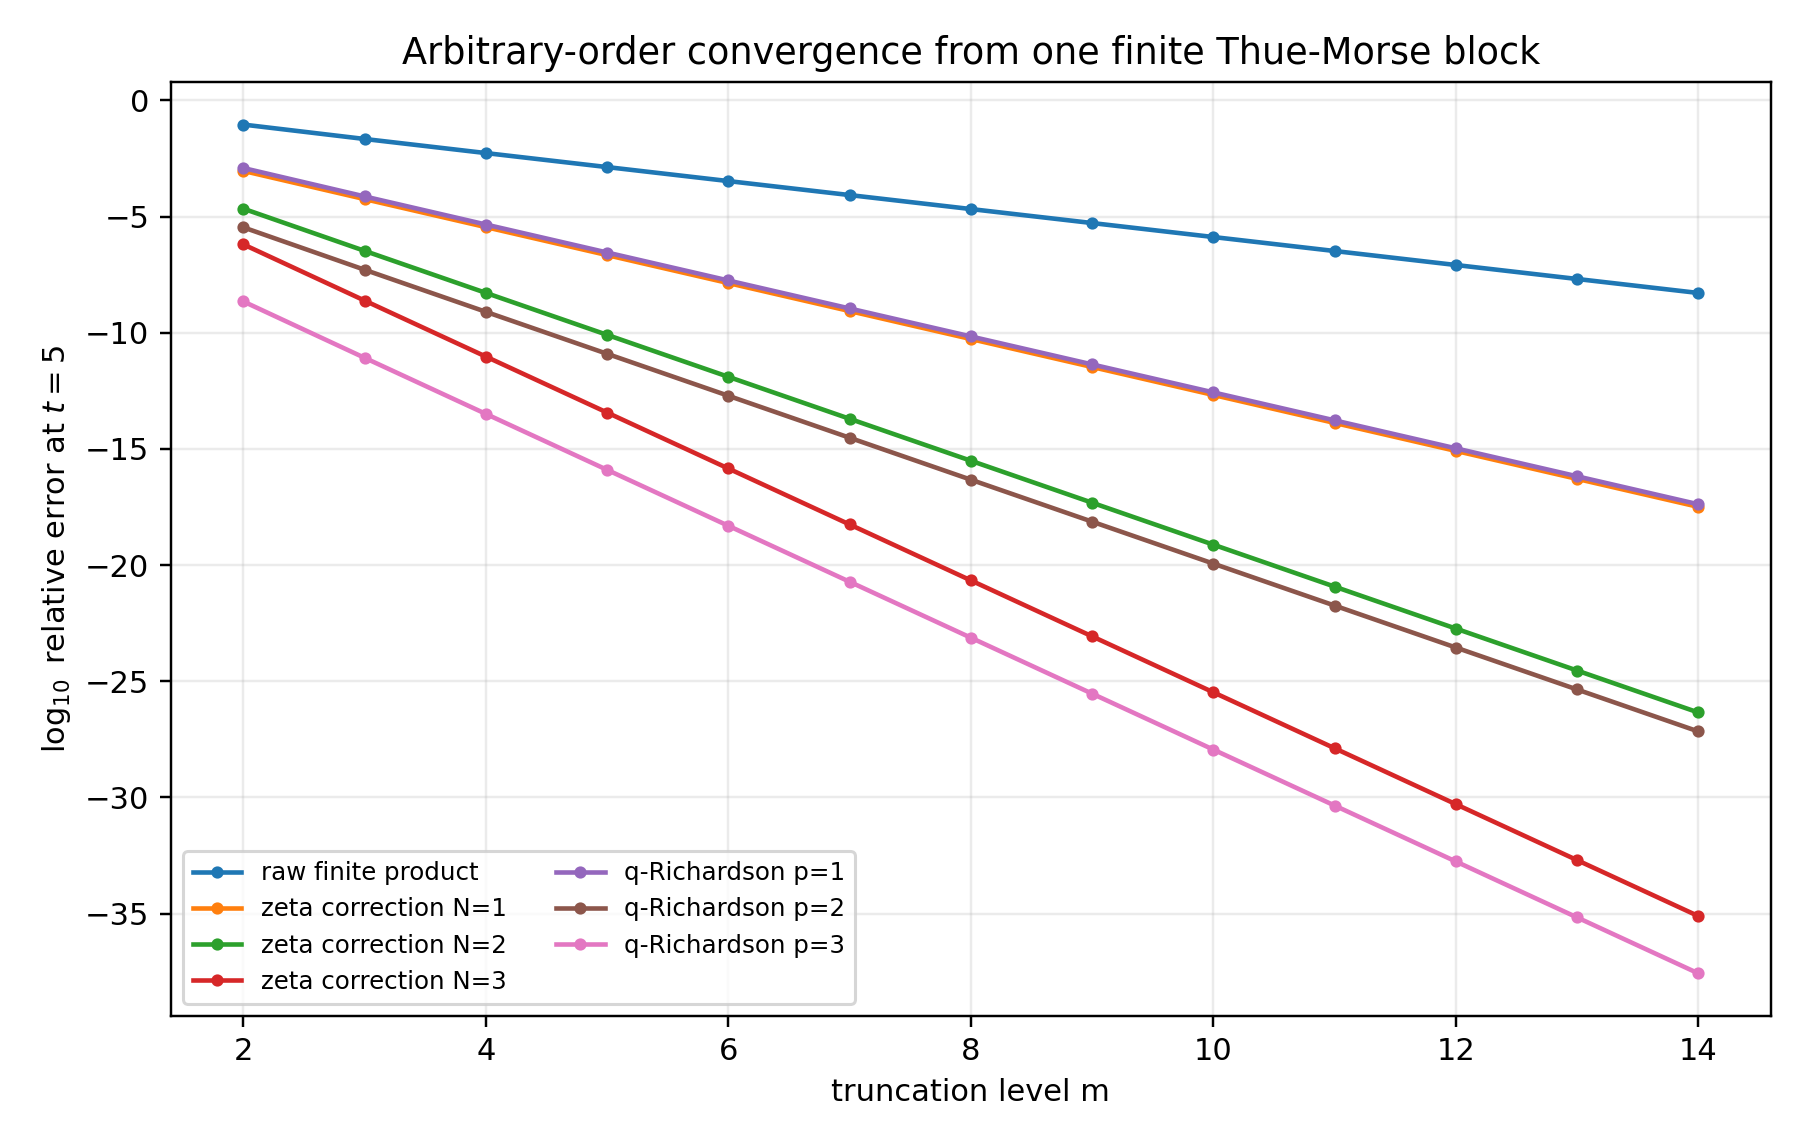
\includegraphics[width=0.97\textwidth]{assets/Fabius_Rvachev_Thue_Morse_Frontier_Results/figures/spectral_convergence.png}
\caption{Relative errors at $t=5$.  Every zeta correction or Richardson degree raises the
power of $4^{-m}$ by one, exactly as predicted by
\cref{p2:cor:arbitrary-Q,p2:thm:qRichardson}.}
\label{p2:fig:spectral-convergence}
\end{figure}

A least-squares fit to the final five points of each curve gives:
\begin{center}
\small
\begin{tabular}{@{}lcc@{}}
\toprule
method & fitted order in $4^{-m}$ & proved order \\
\midrule
raw $Q_m$ & $1.00000013$ & $1$\\
zeta correction $N=1$ & $2.00000006$ & $2$\\
zeta correction $N=2$ & $3.00000007$ & $3$\\
zeta correction $N=3$ & $4.00000008$ & $4$\\
$q$-Richardson $p=1$ & $2.00000014$ & $2$\\
$q$-Richardson $p=2$ & $3.00000013$ & $3$\\
$q$-Richardson $p=3$ & $4.00000013$ & $4$\\
\bottomrule
\end{tabular}
\end{center}

\subsection{Weak expansion check}

For $\varphi(y)=\e^y$, all derivatives equal $\e^y$, so
\cref{p2:thm:weak-expansion} becomes a direct moment correction to the finite moment-generating
function.  The relative errors are:
\begin{center}
\small
\begin{tabular}{@{}rcccc@{}}
\toprule
$m$ & raw spline & through $\mu_2$ & through $\mu_4$ & through $\mu_6$\\
\midrule
2 & $3.465\times10^{-3}$ & $4.569\times10^{-6}$ & $3.311\times10^{-9}$ & $1.540\times10^{-12}$\\
4 & $2.170\times10^{-4}$ & $1.789\times10^{-8}$ & $8.105\times10^{-13}$ & $2.357\times10^{-17}$\\
6 & $1.356\times10^{-5}$ & $6.991\times10^{-11}$ & $1.979\times10^{-16}$ & $3.597\times10^{-22}$\\
8 & $8.477\times10^{-7}$ & $2.731\times10^{-13}$ & $4.832\times10^{-20}$ & $5.489\times10^{-27}$\\
10 & $5.298\times10^{-8}$ & $1.067\times10^{-15}$ & $1.180\times10^{-23}$ & $8.375\times10^{-32}$\\
\bottomrule
\end{tabular}
\end{center}
Each added even moment raises the order by one power of $4^{-m}$.

\subsection{Endpoint-tail coefficients}

The absolute errors in approximating $\log G(-u)$ by the exact linear term plus the first
$N$ even corrections are:
\begin{center}
\small
\begin{tabular}{@{}rcccc@{}}
\toprule
$u$ & $N=0$ & $N=1$ & $N=2$ & $N=3$\\
\midrule
$0.02$ & $5.56\times10^{-6}$ & $3.70\times10^{-12}$ & $5.60\times10^{-18}$ & $1.04\times10^{-23}$\\
$0.2$ & $5.56\times10^{-4}$ & $3.70\times10^{-8}$ & $5.60\times10^{-12}$ & $1.04\times10^{-15}$\\
$1$ & $1.39\times10^{-2}$ & $2.31\times10^{-5}$ & $8.71\times10^{-8}$ & $4.03\times10^{-10}$\\
$3$ & $1.23\times10^{-1}$ & $1.81\times10^{-3}$ & $6.12\times10^{-5}$ & $2.54\times10^{-6}$\\
\bottomrule
\end{tabular}
\end{center}
The deterioration as $u$ approaches the exact radius $4\pi$ is governed by the certified
bound \eqref{p2:eq:G-rem}.

\subsection{Lambert-depth experiment}

For $x=10^{-8}$,
\[
 \lambda(x)=31.555232088424067978\ldots,
 \qquad s_0(x)=3.1555232088424068\times10^9.
\]

\begin{figure}[htbp]
\centering
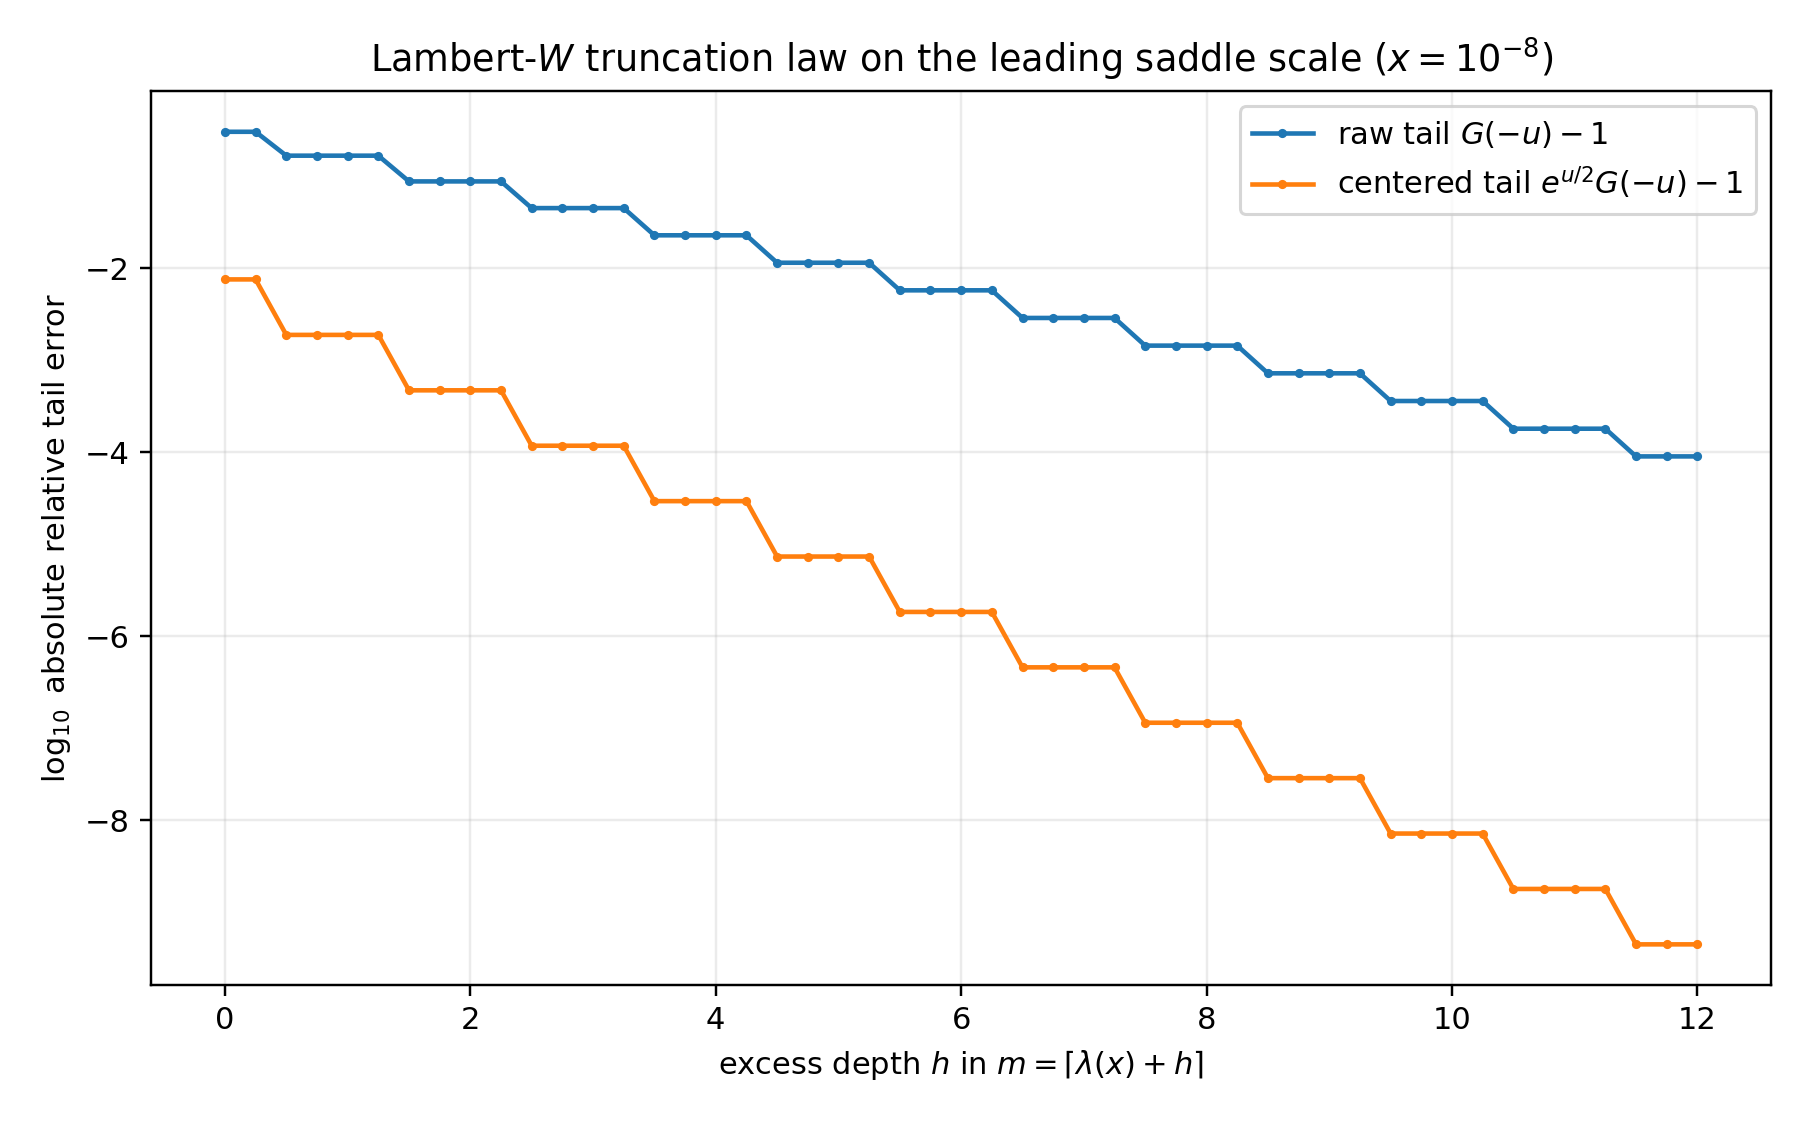
\includegraphics[width=0.97\textwidth]{assets/Fabius_Rvachev_Thue_Morse_Frontier_Results/figures/lambert_truncation.png}
\caption{Tail error when $m=\lceil\lambda(x)+h\rceil$.  Ceiling effects create the steps.
The raw tail gains about one binary digit per extra factor; the centered tail gains about two,
as proved in \cref{p2:thm:depth-law}.}
\label{p2:fig:Lambert-depth}
\end{figure}

At $h=8$, for example, $m=40$ and $u\approx2.8699\times10^{-3}$; the raw tail error is
$1.43\times10^{-3}$ while the centered tail error is $1.14\times10^{-7}$.

\clearpage
\section{Consequences for the existing research program}
\label{p2:sec:consequences}

\subsection{A new exact-arithmetic/Fourier bridge}

The Atlas treats the block polynomial $P_m$ as a digital and algebraic object, while the
Fourier-decay program treats dyadic sinc products through shell dynamics and lacunary sine
products.  Theorem \ref{p2:thm:finite-sinc} shows these are not merely related by analogy:
$P_m$ is the finite sinc product after one explicit normalization.  This provides a direct
translation dictionary:
\begin{center}
\small
\begin{tabular}{@{}ll@{}}
\toprule
finite digital statement & spectral statement \\
\midrule
order-$m$ zero of $P_m$ at $1$ & removable $t^{-m}$ normalization at the origin\\
Thue--Morse exponential sum & truncated up-function Fourier transform\\
Prouhet moment cancellation & high-order low-frequency cancellation\\
block length $2^m$ & product depth $m$\\
geometric error $4^{-m}$ & variance scale of omitted random tail\\
\bottomrule
\end{tabular}
\end{center}

The shell-factorization results remain essential for large real $t$ with $m$ tied to the
frequency shell.  The present tail calculus addresses a different regime: once the first
$m$ factors have been isolated, it computes the remaining small-argument factor to arbitrary
order.  The two analyses are complementary rather than competing.

\subsection{A new $q$-binomial role}

The repository's dyadic arithmetic naturally uses $q=1/2$ because scales and evaluation
points are dyadic.  The present extrapolation naturally uses $q=1/4$ because the centered
error expansion is even.  Gaussian binomials now appear in a second structural role:
\begin{equation}
 \text{exact dyadic values: }q=\frac12,
 \qquad
 \text{spectral-tail acceleration: }q=\frac14.
 \label{p2:eq:two-q}
\end{equation}
This distinction is conceptually useful.  It prevents the $q$-binomial notation from being
viewed as an incidental encoding of one exact formula; it reflects two different geometric
lattices in the same theory.

\subsection{A certified route from finite splines to $\Up$}

The repeated-integration dossiers identify finite stages with compactly supported splines and
prove convergence.  The random-tail theorem strengthens the conceptual picture:
\[
 \text{limit law} = \text{finite spline law} + \text{scaled independent copy of the limit law}.
\]
The weak expansion \eqref{p2:eq:weak-expansion} then supplies every correction coefficient and a
one-line remainder bound.  For numerical integration against smooth observables, the result
is immediately useful: one may integrate against the elementary finite spline $u_m$ and add
explicit derivative corrections, without ever sampling the limiting density directly.

\subsection{A product engine for endpoint saddles}

The endpoint theory's difficult part is the periodically modulated saddle, not the mere
existence of the product.  Nevertheless, every saddle evaluation repeatedly calls the
negative-Laplace product and its derivatives.  Formula \eqref{p2:eq:G-TM-all} suggests a hybrid
implementation:
\begin{enumerate}
\item use the existing lower-Lambert phase and periodic saddle jets to choose $s$;
\item choose $m$ from the centered depth law \eqref{p2:eq:mctr};
\item evaluate the exact finite Thue--Morse block and a few Bernoulli corrections;
\item differentiate the finite factorization rather than the infinite product.
\end{enumerate}
Because $u=s/2^m$ is small by construction, all differentiated correction series remain in a
controlled analytic disk.  This could turn the qualitative endpoint expansion into a
certified high-precision algorithm with transparent complexity.

\subsection{Formalization leverage}

The main new identities have unusually short dependency chains.  The finite bridges are
finite-product algebra.  Tail self-similarity is reindexing.  The weak expansion is Taylor's
theorem plus independence and symmetry.  The $q$-Richardson weights are finite Lagrange
interpolation.  Only the analytic logarithm and explicit zeta remainder require a substantial
complex-analysis layer.  This makes the package a plausible next formalization target --- and
in large part it is not a target at all but already done: as the \emph{Formal version}
paragraphs throughout \cref{p2:sec:objects,p2:sec:bridges,p2:sec:zeta-tail,p2:sec:richardson,p2:sec:gamma-tower}
record, the block identity, both finite bridges in total normalized complex form, with
denominator-free equalities at the origin and quotient corollaries away from zero, both halves of
tail self-similarity, the Fourier--Laplace rotation, the Lagrange characterization of the
$q$-Richardson weights with all three of its moment identities together with their closed
$q$-binomial form (compiled in \path{GeometricQBinomialLagrange.lean}), every spectral
level of the GammaLog/tower Mellin and dyadic laws together with the level-zero
master-product ratio, and now the entire zeta--Lambert tail calculus --- the Euler--zeta
logarithm, the all-orders expansion, the certified remainder, and the exact
prefix--corrections--tail split (\path{EulerLogTransform.lean}, \path{SincZetaSeries.lean},
\path{SincZetaDyadic.lean}, \path{SincZetaRemainder.lean}) --- already have Lean
counterparts, several of them more general than the statements printed here.  The abstract
weighted Richardson tail is now formal under unconditional summability in
\path{AnalyticSeriesFilter.lean}.  Its sinc-product instantiation, ordered and uniform
remainder bounds, and the probabilistic layer are the remaining formalization targets.

\section{Lean formalization roadmap}
\label{p2:sec:formalization}

The finite-block calculus has been deliberately organized so that the algebraic core can be
formalized before the analytic refinements.  The following dependency table separates the
short, high-confidence lemmas from the portions that require additions to the surrounding
analysis library.

Several rows have since been overtaken by the library and are retained because
the table is also a dependency map.  The finite Thue--Morse product
\eqref{p2:eq:Pm} is
\leanPartx{Fabius.prod_one_sub_pow_eq_sum_thueMorseSign}, proved over an arbitrary commutative
ring, not by the coefficient induction suggested below.  The finite sinc and
Laplace bridges \eqref{p2:eq:finite-sinc}--\eqref{p2:eq:finite-Laplace} are now
fully discharged in \path{ThueMorseComplexProductBridge.lean}.  Their primary
equalities are complex and total at the origin; the factors $t^m$ and $s^m$
expose the removable zeros, the prefix-at-zero simp laws give normalized value
one, and the printed quotient normalizations are supplied as corollaries under
the corresponding nonzero hypothesis.  Exact tail self-similarity
\eqref{p2:eq:Q-tail-self}--\eqref{p2:eq:G-tail-self} is fully discharged, and the reusable
reindexing lemma the row asks for is exactly what was proved:
\leanPartx{Fabius.tprod_geom_scale_pow} is stated for an arbitrary function into a commutative
topological monoid.  Of the $q$-Richardson row, the interpolation characterization
\eqref{p2:eq:weights-Lagrange} and the moment identities
\eqref{p2:eq:moment-cancel}--\eqref{p2:eq:first-uncancelled}, the forward
Gaussian-binomial normalization \eqref{p2:eq:weights}, and the complete
coefficientwise action on formal power series are now delivered at arbitrary
ratio.  The last item is the generic diagonal-filter API of
\path{FinitePowerSeriesFilter.lean} and its geometric residual specialization
\path{GeometricPowerSeriesFilter.lean}.  The companion
\path{AnalyticSeriesFilter.lean} evaluates an abstract coefficient series
directly and gives the exact Gaussian tail whenever every contributing sample
is unconditionally summable; zero weights impose no unweighted convergence
condition.  It excludes conditionally-only boundary series and does not connect
the abstract coefficients to the sinc product.  The Euler--zeta logarithm and certified zeta remainder
have likewise since been delivered in \path{SincZetaSeries.lean} and
\path{SincZetaRemainder.lean}, and the random-tail law exists in measure form in
\path{MeasureRefinement.lean}.  What remains includes the concrete sinc-product
Richardson identification, weighted uniform remainder and convergence theorem,
the random-variable weak expansion, the Lambert depth law, and the
parameter-\(a\) differential and iterated differential Gamma-tower ladder.
In particular, neither the formal filter identity
nor the abstract unconditionally summable tail implies the analytic bounds or
brackets stated later in this part.

\begingroup
\small
\setlength{\LTleft}{0pt}
\setlength{\LTright}{0pt}
\begin{longtable}{@{}p{0.20\textwidth}p{0.24\textwidth}p{0.50\textwidth}@{}}
\toprule
Target & Minimal ingredients & Suggested proof strategy and principal risk \\
\midrule
\endfirsthead
\toprule
Target & Minimal ingredients & Suggested proof strategy and principal risk \\
\midrule
\endhead
Finite Thue--Morse product
\eqref{p2:eq:Pm} & finite products, binary recursion, geometric sums & Prove
$P_{m+1}(z)=P_m(z)(1-z^{2^m})$ and identify coefficients by induction.  This should be almost
entirely algebraic. \\
Finite sinc bridge
\eqref{p2:eq:finite-sinc} & complex exponential identities, finite-product
reindexing & \emph{Delivered} in \path{ThueMorseComplexProductBridge.lean}:
the all-level total equality is
\leanPartx{Fabius.thueMorseBlock_cexp_eq_sincPrefix}, its positive-level atlas
wrapper is \leanPartx{Fabius.thueMorseBlock_cexp_eq_sincPrefix_of_pos}, and the
quotient and origin laws are
\leanPartx{Fabius.shiftedComplexSincPrefix_eq_thueMorseBlock_cexp_of_pos} and
\leanPartx{Fabius.shiftedComplexSincPrefix_apply_zero}. \\
Finite Laplace bridge
\eqref{p2:eq:finite-Laplace} & complex exponentials, finite products &
\emph{Delivered} in \path{ThueMorseComplexProductBridge.lean} by
\leanPartx{Fabius.thueMorseBlock_exp_neg_eq_laplacePrefix}, with quotient
corollary \leanPartx{Fabius.complexLaplacePrefix_eq_thueMorseBlock_exp_neg}
and origin law \leanPartx{Fabius.complexLaplacePrefix_apply_zero}; the same
module proves the finite Fourier--Laplace rotation in
\leanPartx{Fabius.complexLaplacePrefix_eq_exp_mul_shiftedComplexSincPrefix}. \\
Exact tail self-similarity
\eqref{p2:eq:Q-tail-self}--\eqref{p2:eq:G-tail-self} & convergence of infinite products, shifted
indices & Establish a reusable infinite-product reindexing lemma.  Existing repository
convergence results should discharge the side conditions. \\
Euler--zeta logarithm
\eqref{p2:eq:logsinc} & local analytic logarithm, Euler's sine product, normal convergence &
\emph{Delivered} in \path{SincZetaSeries.lean} (exponential and real-logarithm forms), on
the general Euler log transform of \path{EulerLogTransform.lean}; the all-orders identity
\eqref{p2:eq:Q-all-orders} is \path{SincZetaDyadic.lean}. \\
Certified zeta remainder
\eqref{p2:eq:Q-remainder-bound} & positivity, monotonicity of $\zeta(2r)$, geometric series &
\emph{Delivered} in \path{SincZetaRemainder.lean}: the verbatim bound, real-argument
nonnegativity, and the exact prefix--corrections--tail split. \\
$q$-Richardson weights
\eqref{p2:eq:weights}--\eqref{p2:eq:first-uncancelled} & finite Lagrange interpolation,
$q$-Pochhammer algebra & \emph{Delivered} in
\path{GeometricQBinomialLagrange.lean}: zero-extended numerator in both
forward and reversed Gaussian forms, the reversed denominator-free polynomial,
normalized weight under node injectivity, and every positive residual moment.
\path{GeometricPowerSeriesFilter.lean} further packages the entire
coefficientwise filter, while \path{AnalyticSeriesFilter.lean} supplies the exact
unconditionally summable analytic Gaussian tail and its shifted-scale form,
with convergence required only for nonzero-weight samples.  Conditional boundary
summation, the sinc-product coefficient bridge, and ordered or uniform remainder
bounds are not part of this row.  The case \(q=1/2\) is linked to the Toeplitz row. \\
Random-tail law
\eqref{p2:eq:random-tail} & independent random variables, almost-sure summation, equality in law &
\emph{Delivered} in measure form in \path{MeasureRefinement.lean}, by exactly the
characteristic-function route this row predicted: the refinement equation and its
$m$-fold iterate, via \leanPartx{charFun\_conv} and the formal Fourier product. \\
Weak expansion
\eqref{p2:eq:weak-expansion} & Taylor theorem with remainder, expectation inequalities, symmetry &
Condition on the finite sum; use bounded support to make the remainder estimate immediate. \\
Lambert depth law
\eqref{p2:eq:mraw}--\eqref{p2:eq:mctr} & branch $W_{-1}$, ceilings, local exponential estimates & The
analytic estimate is elementary after the definition of $\lambda$; the likely missing piece is
a convenient formal API for the lower real Lambert branch. \\
Thue--Morse gamma tower
\eqref{p2:eq:gamma-Mellin}--\eqref{p2:eq:gamma-iterated} & reciprocal-Gamma
first jets, Atlas Dirichlet continuation, parameter differentiation &
\emph{Mellin and dyadic layers delivered}: \path{ReciprocalGammaJets.lean}
proves the exact simple reciprocal-Gamma jet at every nonpositive integer, and
\path{ThueMorseGammaTower.lean} proves every continuation first jet, the
Mellin/integral GammaLog levels, both dyadic laws, and the level-zero
master-product ratio.  Only \eqref{p2:eq:gamma-differential}--\eqref{p2:eq:gamma-iterated}
remain; they need a parameter-under-the-Mellin-integral theorem. \\
\bottomrule
\end{longtable}
\endgroup

A practical promotion sequence is therefore
\[
 \boxed{\begin{gathered}
 \text{finite bridges}
 \longrightarrow \text{tail reindexing}
 \longrightarrow \text{probabilistic splitting}\\
 \longrightarrow \text{$q$-interpolation}
 \longrightarrow \text{analytic logarithms}
 \end{gathered}}
\]
The first four stages already yield exact identities and acceleration mechanisms.  The final
stage adds the sharp radius and explicit zeta remainder.  This ordering minimizes the amount
of new complex analysis that must be trusted at any one time.  Every stage of the boxed
chain now has a formal counterpart (see the \emph{Formal version} paragraphs above): the
finite bridges, tail reindexing, $q$-interpolation, and analytic logarithms directly, and
the probabilistic splitting twice over --- in measure form
(\path{MeasureRefinement.lean}) and, through the affine bridge
\(\mu_{\Up}=\operatorname{law}(X_\infty)\circ(2\cdot{}-1)^{-1}\), where
\(X_\infty=(Y_\infty+1)/2\), as the equality-in-law
splitting of the random series itself (\path{RandomSeriesLaw.lean}).  Every stage of the
chain is formal.

\begin{obligation}[Canonical normalization theorem --- discharged]
The repository uses several Fourier-transform conventions across historical manuscripts.
A promoted theorem should package the convention explicitly and derive all rescalings between
$F$, $\Up$, $Q_\infty$, and the characteristic function of $Y_\infty$.  Doing so would prevent
sign and $2\pi$ factors from leaking into later shell or saddle arguments.
\end{obligation}

This obligation is now discharged: \leanPartx{Fabius.normalization\_dictionary} in
\path{NormalizationDictionary.lean} is the promoted package.  Its four conjuncts fix the
convention \(\widehat{\Up}(z)=\int_\R\Up(t)\e^{-2\pi\ii tz}\dd t\) and derive every rescaling
simultaneously: the function-level fold \(\Up=F(1-|\cdot|)\) (also promoted separately as
\leanPartx{Fabius.rvachevUp\_eq\_fabiusReal\_one\_sub\_abs}), the product identity
\(\widehat{\Up}=Q_\infty\) on all of \(\C\), the centered characteristic function
\(\mathbb{E}[e^{itY_\infty}]=\widehat{\Up}(t/(2\pi))\), and the uncentered
\(\mathbb{E}[e^{itX_\infty}]=e^{it/2}\,\widehat{\Up}(t/(4\pi))\).  The individual legs that fix the
convention remain available: \leanPartx{Fabius.rvachevFourier} is
$\int_\R\Up(t)\e^{-2\pi\ii tz}\dd t$,
\leanPartx{Fabius.rvachevFourier_eq_product} converts it into $Q_\infty$, and
\leanPartx{Fabius.complexGeneratingFunction_eq_fourier_analytic} together with
\leanPartx{Fabius.complexGeneratingFunction_neg_eq_tprod} carries the rotation to $G$.  The
characteristic-function leg is now formal as well:
\leanPartx{Fabius.charFun\_weightedSumDistribution} evaluates
\(\mathbb{E}[e^{itX_\infty}]=e^{it/2}\,\widehat{\Up}(t/(4\pi))\) for the uncentered
\(X_\infty=(Y_\infty+1)/2\), while
\leanPartx{Fabius.rvachevMeasure\_charFun\_pos} gives the centered identity
\(\mathbb{E}[e^{itY_\infty}]=\widehat{\Up}(t/(2\pi))\).  These fix the rescaling between
Mathlib's characteristic-function convention and \leanPartx{Fabius.rvachevFourier}, with
the \(F\leftrightarrow\Up\) passage carried at measure level by
\leanPartx{Fabius.rvachevMeasure\_eq\_map\_weightedSum} and its CDF identity
\leanPartx{Fabius.rvachevMeasure\_Iic}.  The packaging the obligation asked for is exactly the four
conjuncts of \leanPartx{Fabius.normalization\_dictionary}: later shell or saddle arguments
can cite the dictionary instead of reassembling sign and \(2\pi\) conventions at each use.

\begin{obligation}[Reusable geometric-tail API --- discharged]
The identity ``tail equals a scaled copy of the whole object'' occurs simultaneously for
products, convolutions, random series, and cumulant generating functions.  A small abstract
library for geometrically self-similar tails would make the dyadic case a specialization
rather than four separate proofs.
\end{obligation}

The product quarter of this obligation is discharged.  \path{GeometricScaleProducts.lean}
is exactly the abstract library asked for on the product side:
\leanPartx{Fabius.tprod_geom_scale} and \leanPartx{Fabius.tprod_geom_scale_pow} are proved for an
arbitrary function from a field into a commutative topological monoid and an arbitrary scale,
with the dyadic sinc shells obtained as specializations, exactly as the obligation proposes.
The logarithmic face of the same abstraction is now \path{EulerLogTransform.lean}: the
transform $\sum_i\log(1-a_i)=-\sum_{r\ge1}\bigl(\sum_ia_i^r\bigr)/r$ for an arbitrary
absolutely summable family with every norm below one, over an arbitrary index type, with the
geometric family --- the self-similar tail par excellence --- as its first instance.
(The negative-Laplace tail \eqref{p2:eq:G-tail-self} is formal too, but as an independent
induction on the functional equation rather than as an instance of that API --- which is
itself a small illustration of the duplication the obligation is about.)  The convolution
quarter is now discharged in the same abstract style:
\path{GeometricConvolutionTails.lean} builds the prefix system \(P_0=\delta_0\),
\(P_{m+1}=\nu\ast T_*P_m\) of an arbitrary digit measure under an arbitrary measurable
additive endomorphism and proves, by pure convolution algebra, the cocycle law
\(P_{m+n}=P_m\ast(T^m)_*P_n\) (\leanPartx{Fabius.digitPrefix\_add}) and the geometric tail
law --- from the one-step refinement \(\mu=\nu\ast T_*\mu\) alone, \(\mu=P_m\ast(T^m)_*\mu\)
for every \(m\) (\leanPartx{Fabius.self\_similar\_conv\_iterate}) --- together with the
real-scale specialization and the finite product formula
\(\operatorname{charFun}(P_m)(t)=\prod_{k<m}\operatorname{charFun}\nu(c^kt)\)
(\leanPartx{Fabius.charFun\_mulPrefix}).  The dyadic instance \eqref{p2:eq:density-deconv}
is a specialization: \path{MeasureRefinement.lean} now derives the measure-level
random-tail law \eqref{p2:eq:random-tail} from the refinement equation through this API
(see the \emph{Formal version} paragraph in \cref{p2:sec:probability}), and the
random-variable representation underlying it is \path{ProbabilityRepresentation.lean},
with the equality-in-law splitting in \path{RandomSeriesLaw.lean}.  The cumulant
quarter is now formal as well: \path{GeometricCgfTails.lean} proves the moment tail law
unconditionally (the moment generating function of a convolution factors with no
integrability hypotheses, \leanPartx{Fabius.mgf\_id\_conv} and
\leanPartx{Fabius.mgf\_id\_self\_similar}), the cumulant tail law
\(K_\mu(t)=\sum_{k<m}K_\nu(c^kt)+K_\mu(c^mt)\) under finite exponential moments
(\leanPartx{Fabius.cgf\_id\_self\_similar}), and the dyadic instance with every
hypothesis discharged by compact support
(\leanPartx{Fabius.cgf\_uniformDigitPrefix},
\leanPartx{Fabius.cgf\_rvachevMeasure\_self\_similar}).  With that, each of the four
faces has the abstract library the obligation asked for, with the dyadic case a
specialization, and the obligation is discharged.  The single statement instantiating
to all four faces at once now exists as well: \path{GeometricTailDictionary.lean} proves
\leanPartx{Fabius.geometric\_tail\_dictionary} --- from the one-step refinement
\(\mu=\nu\ast(c\cdot)_*\mu\) alone, one theorem with four conjuncts: the measure face
\(\mu=P_m\ast(c^m\cdot)_*\mu\), the product face \(\varphi_\mu(t)=\bigl(\prod_{k<m}\varphi_\nu(c^kt)\bigr)\,\varphi_\mu(c^mt)\)
(whose assembly \leanPartx{Fabius.charFun\_self\_similar} it also provides), the unconditional
moment face, and the cumulant face under finite exponential moments --- with the dyadic
instance \leanPartx{Fabius.geometric\_tail\_dictionary\_up} carrying every hypothesis
discharged by compact support.  The operator-exponential display
\eqref{p2:eq:cumulant-operator} is now formal at exactly the level the remark asserts it:
\path{SmoothingOperatorExponential.lean} proves that for any zero-constant exponent
series over a rational algebra, the smoothing operator of its generated exponential
acts on every polynomial as the finite (degreewise-nilpotent) exponential of the
exponent's operator,
\(\mathcal S_{\exp K}\,q=\sum_{d\le\deg q}\tfrac1{d!}\,\mathcal S_K^{\,d}\,q\)
(\leanPartx{Fabius.seriesDerivOp\_expSeries}, with the coefficient identity
\leanPartx{Fabius.expCoeff\_eq\_sum\_coeff\_pow} and the vanishing of low coefficients
of powers of a zero-constant series) --- expanding the exponential changes cumulants
into moments exactly as claimed, with the Fabius instance available through the
moment--cumulant dictionary of \path{MomentCumulantAlgebra.lean}.  Only the
distributional reading of \eqref{p2:eq:cumulant-operator} against the spline densities
remains analytic.

\section{Frontier conjectures and next deductions}
\label{p2:sec:frontiers}

The proved results isolate several questions which are both sharper and more tractable than
the broad open-ended prompts in the older frontier notebooks.  The statements below are
intentionally separated from the theorem package.

\begin{conjecture}[Certified endpoint evaluator with near-optimal product depth]
\label{p2:conj:endpoint-evaluator}
There is a fully explicit algorithm which, for sufficiently small $x>0$ and target relative
error $\eta$, evaluates $F(x)$ using
\begin{equation}
 -\frac{W_{-1}(-x\log2)}{\log2}
 +\frac12\log_2\frac1\eta+\bigO(1)
 \label{p2:eq:conj-depth}
\end{equation}
product layers, together with a bounded-order periodic saddle jet, and whose final error is
rigorously at most $\eta$.  The coefficient $1/2$ in the precision surcharge is optimal among
methods which first center the omitted product but do not cancel its quadratic cumulant.
\end{conjecture}

The depth estimate itself is proved in \cref{p2:thm:depth-law}.  What remains is to propagate the
product error, its differentiated versions, and the periodic saddle displacement through the
complete inversion formula.  The conjectured optimality should follow from the nonzero
variance $\kappa_2=1/9$.

\begin{conjecture}[Cumulant-cancelled endpoint hierarchy]
\label{p2:conj:cumulant-depth}
After removing the first $N$ even cumulants of the centered tail in addition to the linear
factor, the extra depth required for tolerance $\eta$ is
\begin{equation}
 \frac{1}{2N+2}\log_2\frac1\eta+\bigO_N(1).
 \label{p2:eq:cumulant-depth-conj}
\end{equation}
Equivalently, the $N$-corrected finite block should require only one additional product layer
for every $2N+2$ requested binary digits of tail accuracy.
\end{conjecture}

This is already a theorem for the isolated product, by \eqref{p2:eq:G-rem}; the conjectural part
is that the same saving survives uniformly through the full saddle inversion, including all
needed derivatives and the periodic phase.

\begin{conjecture}[Strong spline correction away from knots]
\label{p2:conj:strong-spline}
Fix $N\ge0$ and a compact interval $K\subset(-1,1)$.  After excluding a neighborhood of the
knots of the finite spline $u_m$ whose width is comparable to $2^{-m}$, the distributional
expansion \eqref{p2:eq:distributional} admits a pointwise or Hölder-norm version through order
$N$, with remainder $\bigO_K(4^{-(N+1)m})$ after the natural derivative scaling.
\end{conjecture}

A global pointwise statement cannot be obtained by naively differentiating $u_m$: finite
splines have knots, whereas $\Up$ is smooth.  The random-tail convolution indicates two viable
repairs.  One may either retain the exact final mollifier $2^m\Up(2^m\cdot)$, or state the
expansion on cells separated from their endpoints.  Establishing the best norm and boundary
layer is a concrete approximation-theoretic problem.

\begin{conjecture}[Dual-$q$ transmutation]
\label{p2:conj:dual-q}
There is a direct coefficient-level transform taking a substantial class of the repository's
$q=1/2$ exact dyadic formulae into $q=1/4$ spectral-tail acceleration identities, with the
squaring $q\mapsto q^2$ explained by parity or centering rather than by an ad hoc substitution.
\end{conjecture}

Evidence is structural: the exact dyadic theory resolves single binary scales, while every
centered Fourier or probability correction is even and therefore sees squared scales.  A
useful form of the conjecture would turn Gaussian-binomial coefficient extraction at
$q=1/2$ into geometric-grid interpolation at $q=1/4$.

\begin{conjecture}[Automatic Barnes hierarchy]
\label{p2:conj:automatic-Barnes}
The functions $\Gamma_r^{\rm TM}$ possess canonical Weierstrass products and asymptotic
normalizations for which the dyadic law \eqref{p2:eq:gamma-dyadic} and differential ladder
\eqref{p2:eq:gamma-differential} uniquely characterize the hierarchy, analogously to the role of
convexity or normalization in classical gamma-type characterizations.
\end{conjecture}

The Mellin formula gives positivity and complete-monotonicity information for suitable signed
derivatives, while the dyadic equation supplies an automatic analogue of a multiplication
formula.  The remaining difficulty is to choose a normalization that removes the freedom to
multiply by functions invisible to the differential recursion.

\subsection{General radix and nonuniform tails}

The base-$b$ theorem \eqref{p2:eq:base-b} shows that the zeta--Lambert mechanism does not depend
on binary arithmetic.  What is special to base two is the simultaneous existence of the
Thue--Morse block polynomial, the simple two-branch functional equation, and the Fabius/up
probability model.  A next generalization is to replace the uniform summands by centered
compactly supported variables $X_k$ at scales $b^{-k}$.  If their common characteristic
function has a nonzero analytic germ at the origin, then
\[
 \log\frac{\Phi_\infty(t)}{\Phi_m(t)}
 =\sum_{r\ge1}c_r t^r\frac{b^{-r(m+1)}}{1-b^{-r}}.
\]
Thus Lambert kernels are universal for geometric random tails; the zeta values in the present
report are the special signature of the uniform law through Euler's sine product.  The
classification of digital substitutions whose finite block polynomial exactly realizes such
a characteristic product is a natural interface between automatic sequences and compactly
supported refinable laws.

\section{Conclusion}
\label{p2:sec:conclusion}

The documentation corpus already supplied the large pieces: a careful separation of the
Fabius and up-function normalizations, an exact dyadic arithmetic theory rich in
$q$-binomial coefficients, a probabilistic convolution model, a detailed analysis of the
infinite sinc product, corrected lower-Lambert endpoint asymptotics, and a broad Thue--Morse
formula atlas.  The missing junction was finite-block calculus.

One polynomial now connects the principal domains:
\[
 \boxed{
 \begin{array}{c}
 P_m(z)=\displaystyle\sum_{n<2^m}\eps_nz^n\\[0.3em]
 \rotatebox{90}{$=$}
 \end{array}
 \quad
 \begin{array}{c}
 \text{finite digital block}\\
 \text{finite Fourier sinc product}\\
 \text{finite negative-Laplace product}
 \end{array}}
\]
after explicit phase and scale normalizations.  The omitted object is always a scaled copy of
the full object.  That observation produces exact all-order tails, zeta--Lambert coefficients,
Gaussian-binomial extrapolation, random-tail deconvolution, and Lambert-$W$ complexity laws
from a common source rather than as isolated formulas.

The principal proved advances are:
\begin{enumerate}
\item exact oscillatory and decaying substitutions converting a length-$2^m$ Thue--Morse block
      into the first $m$ factors of the Fourier and endpoint products;
\item a convergent all-orders logarithmic tail with exact radius and an explicit geometric
      remainder bound;
\item arbitrary-order corrected finite-block approximants and a separate $q$-Richardson
      scheme whose weights are Gaussian binomials at $q=1/4$;
\item an exact independent-copy decomposition of the omitted random tail, yielding a certified
      weak differential expansion of the up-law in finite uniform splines;
\item raw, centered, and higher-correction product-depth laws on the canonical lower-Lambert
      saddle scale;
\item a Thue--Morse gamma tower obtained by differentiating the entire shifted Dirichlet
      function at its trivial zeros.
\end{enumerate}

These results do not replace the repository's sharp shell dynamics or periodically modulated
endpoint saddle.  They add a complementary local engine: after a finite block or finite shell
has been isolated, the remainder is computable to arbitrary order with transparent constants.
That engine is algebraically short, numerically stable after centering, and unusually suitable
for formal verification.

\appendix
\clearpage
\section{Coefficient and extrapolation tables}
\label{p2:app:coefficients}

\subsection{Zeta--Lambert and centered Laplace coefficients}

Write
\[
 a_r=\frac{\zeta(2r)}{r\pi^{2r}(4^r-1)},
 \qquad
 c_r=\frac{B_{2r}}{2r(2r)!(4^r-1)}.
\]
Then
\[
 \log\frac{Q_\infty(t)}{Q_m(t)}=-\sum_{r\ge1}a_rt^{2r}4^{-rm},
 \qquad
 \log C(-u)=\sum_{r\ge1}c_ru^{2r}.
\]
The first eight exact coefficients are:
\begin{center}
\small
\begin{tabular}{@{}rll@{}}
\toprule
$r$ & $a_r$ & $c_r$\\
\midrule
1 & $1/18$ & $1/72$\\
2 & $1/2700$ & $-1/43200$\\
3 & $1/178605$ & $1/11430720$\\
4 & $1/9639000$ & $-1/2467584000$\\
5 & $1/478533825$ & $1/490018636800$\\
6 & $691/15688261338750$ & $-691/64259118443520000$\\
7 & $2/2092151286225$ & $1/17138903336755200$\\
8 & $3617/170727360353550000$ & $-3617/11188788288130252800000$\\
\bottomrule
\end{tabular}
\end{center}
The numerators $691$ and $3617$ are the familiar Bernoulli numerators; here they enter through
the uniform-tail cumulants rather than through an independent number-theoretic construction.

\subsection{Analytic error germ}

For
\[
 H_t(r)=\frac1{Q_\infty(t\sqrt r)}=\sum_{n\ge0}h_n(t)r^n,
\]
the first coefficients are monomials in $t^2$:
\begin{align*}
 h_0(t)&=1,\\
 h_1(t)&=\frac{t^2}{18},\\
 h_2(t)&=\frac{31t^4}{16200},\\
 h_3(t)&=\frac{2347t^6}{42865200},\\
 h_4(t)&=\frac{1904369t^8}{1311675120000},\\
 h_5(t)&=\frac{3309760579t^{10}}{88561680752160000}.
\end{align*}
They are complete exponential Bell polynomials in $a_1t^2,a_2t^4,\ldots$.  Consequently,
all leading constants in \eqref{p2:eq:Richardson-leading} are exact rational multiples of
$Q_\infty(t)t^{2p+2}$.

\subsection{Gaussian-binomial extrapolation weights}

At $q=1/4$, the first six rows are:
\begin{align*}
 p=0:&\quad (1),\\
 p=1:&\quad \left(-\frac13,\frac43\right),\\
 p=2:&\quad \left(\frac1{45},-\frac49,\frac{64}{45}\right),\\
 p=3:&\quad \left(-\frac1{2835},\frac4{135},-\frac{64}{135},
                         \frac{4096}{2835}\right),\\
 p=4:&\quad \left(\frac1{722925},-\frac4{8505},\frac{64}{2025},
                         -\frac{4096}{8505},\frac{1048576}{722925}\right),\\
 p=5:&\quad \left(-\frac1{739552275},\frac4{2168775},-\frac{64}{127575},
                         \frac{4096}{127575},-\frac{1048576}{2168775},
                         \frac{1073741824}{739552275}\right).
\end{align*}
The alternating signs are unavoidable because the formula extrapolates from positive nodes
$q^m,\ldots,q^{m+p}$ to the endpoint $0$.  For numerical work at very high $p$, barycentric or
compensated summation should be used rather than forming the rational coefficients in floating
point.

\section{Reproducibility protocol}
\label{p2:app:reproducibility}

The numerical checks used direct high-precision arithmetic and did not fit coefficients that
were subsequently inserted into proofs.  The following pseudocode records the independent
verification path.

\begin{lstlisting}[style=pseudo,language=Python,caption={Independent verification skeleton}]
set_precision(100)

def epsilon(n):
    return (-1) ** binary_digit_sum(n)

def P(m, z):
    return product(1 - z ** (2 ** j) for j in range(m))

def Q_finite(m, t):
    return product(sinc(t / (2 ** k)) for k in range(1, m + 1))

def Q_infinite(t, cutoff):
    return product(sinc(t / (2 ** k)) for k in range(1, cutoff + 1))

# Exact finite identities
for (m, t) in test_grid:
    lhs = P(m, exp(1j * t / (2 ** (m - 1))))
    rhs = ((-1j) ** m * t ** m * 2 ** (-m * (m - 1) / 2)
           * exp(1j * t * (1 - 2 ** (-m))) * Q_finite(m, t))
    report(relative_residual(lhs, rhs))

# All-order tail and q-Richardson slopes
for m in depth_grid:
    exact = Q_infinite(t, large_cutoff)
    for N in correction_orders:
        approx = Q_finite(m, t) * exp(-sum(a(r) * t ** (2*r)
                                               * 4 ** (-r*m)
                                               for r in range(1, N + 1)))
        save_error(m, N, relative_error(approx, exact))
    for p in extrapolation_orders:
        approx = sum(weight(p, j) * Q_finite(m + j, t)
                     for j in range(p + 1))
        save_error(m, p, relative_error(approx, exact))
fit_final_log_slopes()

# Random-tail weak expansion, phi(y)=exp(y)
for m in depth_grid:
    finite_mgf = product(sinh(2 ** (-k)) / (2 ** (-k))
                         for k in range(1, m + 1))
    corrected = finite_mgf * sum(moment(2*j) * 4 ** (-j*m)
                                 / factorial(2*j) for j in range(N + 1))
    compare_with_infinite_mgf(corrected)
\end{lstlisting}

The oscillatory and Laplace finite identities were tested at levels up to $m=12$ with relative
residuals between $10^{-96}$ and $10^{-102}$.  Regression was used only to diagnose the
convergence exponent after the formulas had been proved; the fitted base-$4$ orders were
$1,2,3,4$ to roughly seven significant digits for the raw, first-, second-, and third-order
schemes.  The figures embedded in this report were generated from the same data.

\section{Complete corpus ledger and deduplication map}
\label{p2:app:ledger}

\subsection{Living documentation treated as authoritative}

The audit covered every TeX manuscript in the living documentation tree.  At the snapshot date,
the principal paths and roles were:

\begin{longtable}{@{}p{0.42\textwidth}p{0.52\textwidth}@{}}
\toprule
Path or group & Role in the audit\\
\midrule
\endfirsthead
\toprule
Path or group & Role in the audit\\
\midrule
\endhead
\path{Fabius_Function_and_Rvachev_Up/Fabius_Function_and_Rvachev_Up.tex}
& Primary synthesis: normalization, probability, Fourier theory, exact dyadic values, and
corrected endpoint asymptotics.\\
\path{FabiusFunction_Mathematical_Glossary/FabiusFunction_Mathematical_Glossary.tex}
& Terminology and notation cross-check.\\
\path{Non_Elementarity_of_the_Fabius_Function/Non_Elementarity_of_the_Fabius_Function.tex}
& Differential-algebraic and non-elementarity context.\\
\path{fabius_lean_walkthrough/fabius_lean_walkthrough.tex}
& Map between human mathematics, Lean files, dependencies, and proof status.\\
\path{non-formalized-research-frontiers/non-formalized-research-frontiers.tex}
& Consolidated gap register and non-formalized frontier synthesis.\\
\path{non-formalized-research-frontiers/drafts/thue-morse/Thue_Morse_Atlas_and_Frontiers/Thue_Morse_Atlas_and_Frontiers.tex}
& Current consolidated Thue--Morse volume; Part~I is the comprehensive formula atlas and
principal source for the block polynomial and shifted Dirichlet continuation.\\
\path{non-formalized-research-frontiers/drafts/rvachev_up_fourier_decay/}
& Twelve active manuscripts: the initial wave, comparative and second-wave audits, a gentle
guide, the asymptotic-product problem statement, successive waves 2--8, and the final
resolution.  They were compared rather than collapsed because their hypotheses and correction
histories differ.\\
\path{papers/AIF_76_21-38/}
& Original and corrected TeX transcriptions of Arias de Reyna's compact-support paper.\\
\path{papers/arXiv-1502.06738/}
& Source TeX for Aistleitner--Hofer--Larcher on parametric Thue--Morse sequences and lacunary
trigonometric products.\\
\path{papers/arXiv-1702.05442/}
& Source TeX for Arias de Reyna's English translation of the 1982 compact-support article.\\
\path{papers/arXiv-1702.06487/}
& Source TeX for Arias de Reyna's arithmetic study of dyadic Fabius values.\\
\path{papers/arXiv-2211.13570/}
& Source TeX for Tóth's shifted and combined Thue--Morse Dirichlet series.\\
\path{papers/ubiq15/ubiq15-corrected.tex}
& Corrected source for imported automatic-sequence background.\\
\bottomrule
\end{longtable}

Within the Fourier-decay group, the inspected subdirectories were
\path{Rvachev_Up_Fourier_Decay-2},
\path{Rvachev_Up_Fourier_Decay-3},
\path{Comparative_Audit},
\path{Gentle_Guide},
\path{Second_Wave_Audit},
\path{asymptotic-decay-rate-of-an-infinite-product-of-sinc-functions},
\path{rvachev_up_fourier_decay-1}, and
\path{rvachev_up_fourier_decay-4} through
\path{rvachev_up_fourier_decay-8}.  Each contains one principal TeX manuscript.

\subsection{Frozen archive represented through provenance}

The archive README states that entries preserve the first-introduced historical document,
that later edits are not separately archived, and that byte-identical copies already present
in the living tree were pruned.  Accordingly, the audit used the following unique historical
entries as a provenance map rather than counting every renamed or duplicated copy as new
mathematical evidence.

\begin{longtable}{@{}p{0.19\textwidth}p{0.75\textwidth}@{}}
\toprule
Archive category & Frozen entries\\
\midrule
\endfirsthead
\toprule
Archive category & Frozen entries\\
\midrule
\endhead
Early notes
& \path{Fabius Asymptotic};
  \path{K-fold summation over the signed Thue-Morse sequence}.\\
Standalone studies
& \path{Non_Elementarity_of_the_Fabius_Function};
  \path{Small_Argument_Asymptotics};
  \path{fabius-inverse-dyadic-closed-form}.\\
Primary exposition
& \path{Fabius_Function_and_Rvachev_Up};
  \path{Fabius_Function_and_Rvachev_Up-2};
  \path{Fabius_Function_and_Rvachev_Up-3};
  \path{Fabius_and_Rvachev_Up-2};
  \path{Fabius_and_Rvachev_up};
  \path{Fabius_function_and_up_function}.\\
Primary supplements
& \path{Fabius_Function_Missing_Parts};
  \path{Fabius_Function_Missing_Parts-2}.\\
$q$-calculus
& \path{Fabius_q_Special_Functions};
  \path{fabius-q-special-functions}.\\
Lean walkthrough
& Two frozen walkthrough variants recorded under the archive's
  \path{lean-walkthrough} category.\\
Glossary
& Two frozen glossary variants recorded under the archive's \path{glossary} category.\\
Research frontiers
& \path{Fabius_Dyadic_Asymptotic_Bridge};
  \path{Fabius_Dyadic_Formulae_and_Alternative_Representations};
  \path{Fabius_Dyadic_Formulae_to_Asymptotics};
  \path{Fabius_Dyadic_q_Connections};
  \path{Fabius_Thue_Morse_Convergence_Rate};
  \path{Fabius_Thue_Morse_Convergence_Rates};
  \path{Primary_Exposition_Gap_Register};
  \path{Repeated_Integration_and_Rvachev_Up};
  \path{Rvachev_Up_from_Repeated_Integration};
  \path{non-formalized-research-frontiers};
  \path{Thue_Morse_Formula_Atlas-1};
  \path{Thue_Morse_Formula_Atlas-2};
  \path{Thue_Morse_Formula_Atlas-3}.\\
\bottomrule
\end{longtable}

This ledger explains the phrase ``all TeX documents'' operationally: every living manuscript
was inspected, every active mutually auditing draft was retained, every imported TeX paper was
included, and frozen historical variants were read through their explicit provenance and
content map so that superseded copies did not distort novelty checks.

\begin{thebibliography}{99}

\bibitem{p2:proveit-primary}
V.~Reshetnikov,
\emph{The Fabius Function and Rvachev's Up-Function: Exact arithmetic, probability, Fourier
analysis, and corrected sharp asymptotics}, living repository manuscript, 2026.
\url{https://github.com/VladimirReshetnikov/ProveIt/blob/main/Analysis/FabiusFunction/docs/Fabius_Function_and_Rvachev_Up/Fabius_Function_and_Rvachev_Up.tex}

\bibitem{p2:proveit-frontiers}
V.~Reshetnikov,
\emph{Non-Formalized Research Frontiers for the Fabius Function}, living repository
manuscript, 2026.
\url{https://github.com/VladimirReshetnikov/ProveIt/blob/main/Analysis/FabiusFunction/docs/non-formalized-research-frontiers/non-formalized-research-frontiers.tex}

\bibitem{p2:proveit-atlas}
V.~Reshetnikov,
\emph{The Thue--Morse Sequence: Formula Atlas and Fabius--Rvachev Frontier Results}, living
repository manuscript, 2026; Part~I contains the unified formula atlas.
\url{https://github.com/VladimirReshetnikov/ProveIt/blob/main/Analysis/FabiusFunction/docs/non-formalized-research-frontiers/drafts/thue-morse/Thue_Morse_Atlas_and_Frontiers/Thue_Morse_Atlas_and_Frontiers.tex}

\bibitem{p2:proveit-fourier}
V.~Reshetnikov,
\emph{The Fourier Decay of Rvachev's Up-Function: Final Resolution}, living repository
manuscript, 2026.
\url{https://github.com/VladimirReshetnikov/ProveIt/blob/main/Analysis/FabiusFunction/docs/non-formalized-research-frontiers/drafts/rvachev_up_fourier_decay/rvachev_up_fourier_decay-5/Rvachev_Up_Fourier_Decay_Final.tex}

\bibitem{p2:proveit-archive}
V.~Reshetnikov,
\emph{Archive of historical document versions}, provenance README, 2026.
\url{https://github.com/VladimirReshetnikov/ProveIt/tree/main/Analysis/FabiusFunction/docs/archive}

\bibitem{p2:arias1982}
J.~Arias de Reyna,
\emph{An infinitely differentiable function with compact support: Definition and properties},
English translation of \emph{Definici\'on y estudio de una funci\'on indefinidamente
diferenciable de soporte compacto}, Rev. Real Acad. Ciencias Madrid \textbf{76} (1982),
21--38; arXiv:1702.05442 (2017).
\url{https://arxiv.org/abs/1702.05442}

\bibitem{p2:arias2017arith}
J.~Arias de Reyna,
\emph{Arithmetic of the Fabius function}, arXiv:1702.06487v3 (2017).
\url{https://arxiv.org/abs/1702.06487}

\bibitem{p2:aistleitner2015}
C.~Aistleitner, R.~Hofer, and G.~Larcher,
\emph{On parametric Thue--Morse sequences and lacunary trigonometric products},
arXiv:1502.06738v2 (2015).
\url{https://arxiv.org/abs/1502.06738}

\bibitem{p2:toth2022}
L.~T\'oth,
\emph{Linear Combinations of Dirichlet Series Associated with the Thue--Morse Sequence},
INTEGERS \textbf{22} (2022), Article 98; arXiv:2211.13570.
\url{https://arxiv.org/abs/2211.13570}

\bibitem{p2:corless1996}
R.~M. Corless, G.~H. Gonnet, D.~E.~G. Hare, D.~J. Jeffrey, and D.~E. Knuth,
\emph{On the Lambert $W$ function}, Advances in Computational Mathematics \textbf{5} (1996),
329--359.
\url{https://doi.org/10.1007/BF02124750}

\bibitem{p2:allouche2003}
J.-P. Allouche and J.~Shallit,
\emph{Automatic Sequences: Theory, Applications, Generalizations}, Cambridge University
Press, 2003.

\end{thebibliography}


\end{document}
